% !TEX program = xelatex
% 3，5，7方程分别做了哪些假设，效果有什么区别.分别是什么方程
% 为什么是弱可压缩
% 状态方程是怎么取的
% 速度压力平衡，压强一定要为0吗

% 创新点：
% 1. 方程
% 1.1 给方程增加粘性
% 1.2 可以用到5方程模型
% 1.3 可以用到欧拉方程
% 2. 算法
% 2.1 可以当做limiter用在DG中
% 2.2 可以使用三阶精度格式
% 3. 网格
% 3.1 可以用到非结构网格
% 4. 理论
% 4.1 给出恰当的函数空间的构造方案
% 4.2 保正限制器对于非多项式也能保精度

% 问题
% 1. 只写一个升阶WENO吗
% 2. 高精度数值格式篇幅很长，需要单独写一章吗
% 3. 密度大于0，c是实数，这个是充要条件吗

% 还需要增加三种重构方法的对比表格
% 还需要增加重构模板的tikz图
% 还需要增加WENO引用数的增长图

% 工作
% 1. 检验代码为什么会在非边界出现负密度
% 2. 改DG代码

%  VOF Level Set是清晰界面方法吗

\documentclass[12pt,a4paper]{article}
\usepackage{ctex, fontenc}
\usepackage{xcolor} % 在latex中使用颜色
\usepackage{booktabs,tabularx,multicol} % 制作表格
\usepackage{framed} % 制作文本框
\usepackage{amsmath,amsthm,amssymb,amsfonts}    % 数学符号与字体
\usepackage{bm} % 提供 \bm 加粗命令
\usepackage{siunitx}
% \usepackage{hyperref}   % 添加超链接
% \hypersetup{hidelinks} 
\usepackage{makecell}
\usepackage[colorlinks=true, linkcolor=blue, citecolor=blue]{hyperref} % 引入 hyperref 包并设置颜色
\usepackage{subcaption}
\usepackage{mathtools}
\usepackage{listings}
\usepackage{xcolor} % 用于设置颜色
\usepackage{tikz}
\usetikzlibrary{patterns, arrows.meta, calc, decorations.pathmorphing, arrows.meta, shapes.geometric, positioning, calc, backgrounds, fit,shapes.misc}
\usetikzlibrary{calc}
\usepackage[paper=a4paper,top= 27.5mm,left=15.7mm,right = 15.7mm, bottom = 27.5mm]{geometry}

\usepackage[ruled,linesnumbered]{algorithm2e}
\usepackage{listings}
\usepackage{xcolor}
% MATLAB 代码样式设置
% \lstset{
%     language=Matlab,                % 设置语言为 MATLAB
%     basicstyle=\ttfamily\small,     % 基本字体样式
%     keywordstyle=\color{blue}\bfseries, % 关键字样式
%     commentstyle=\color{green!50!black}, % 注释样式
%     stringstyle=\color{orange},     % 字符串样式
%     numbers=left,                   % 行号在左侧
%     numberstyle=\tiny\color{gray},  % 行号样式
%     stepnumber=1,                   % 每行显示行号
%     numbersep=5pt,                  % 行号与代码的间距
%     backgroundcolor=\color{white},  % 背景颜色
%     showspaces=false,               % 不显示空格
%     showstringspaces=false,         % 不显示字符串中的空格
%     showtabs=false,                 % 不显示制表符
%     frame=single,                   % 边框样式：single, shadowbox, none
%     rulecolor=\color{lightgray},    % 边框颜色
%     tabsize=4,                      % 制表符大小
%     captionpos=b,                   % 标题位置：t(top), b(bottom)
%     breaklines=true,                % 自动换行
%     breakatwhitespace=false,        % 在空格处换行
%     escapeinside={\%*}{*)}          % 在代码中插入 LaTeX 命令
% }
\usepackage{appendix}   % 附录环境
\usepackage{graphicx}    % 插入照片
\usepackage{float}      % 固定浮动体
\usepackage{lipsum,zhlipsum} %生成一些测试文本
\usepackage{multirow}
\usepackage{tikz}
\usepackage{physics}

% 新增 threorems, lemmas, definitions, remarks 环境
\newtheorem{theorem}{定理}[section]
\newtheorem{lemma}[theorem]{引理}
\newtheorem{definition}[theorem]{定义}
\newtheorem{remark}[theorem]{注}
\newtheorem{property}{特征}
\usepackage{stmaryrd}
\newcommand{\avg}[1]{\langle #1 \rangle}
\newcommand{\jump}[1]{\llbracket #1 \rrbracket}
%---------------优雅的插入MATLAB代码---------%
\usepackage{listings,matlab-prettifier} % MATLAB 美化包
\lstset{
        style=Matlab-editor,
        % numbers      = left,
        % numbersep    = 5pt,
        % numberstyle  = \small\color{red},
        frame        = single,
        keepspaces   = true,
        tabsize      = 4,
}
 
\geometry{a4paper,left=2.5cm,right=2.5cm,top=3cm,bottom=2.5cm,headsep=6mm,foot=10mm,twoside,bindingoffset=1cm}%定义页面


%-------------标题-------------%
\title{硕士毕业论文}
\date{\today}
\author{张阳}

%-----------做一些设置-----------%
\numberwithin{equation}{section}    % 公式标号与section的编号挂钩
\punctstyle{kaiming}    % 调整标点符号大小

%------------自定义一些命令------------%
\newcommand{\upcite}[1]{\textsuperscript{\textsuperscript{\cite{1}}}}



%---------------高亮--------------%
\usepackage{soul}
\addtocounter{MaxMatrixCols}{10}

\usepackage{setspace}
\doublespacing      % 双倍行距

%%%%%%%%%%%%%%%%%%%%%%%%%%%%%%%%%%%%%%%%%%
\usepackage{tikz}
\usepackage{xcolor}
\usepackage{ctex}  % 中文支持
\usetikzlibrary{shapes.geometric, arrows.meta, positioning, fit, backgrounds}
 
% ── 颜色定义 ──────────────────────────────────────────
\definecolor{bluelight}{RGB}{230, 241, 251}
\definecolor{blueborder}{RGB}{24,  95, 165}
\definecolor{bluetext}  {RGB}{12,  68, 124}
\definecolor{corallight}{RGB}{250, 236, 231}
\definecolor{coralborder}{RGB}{153, 60,  29}
\definecolor{coraltext} {RGB}{113, 43,  19}
\definecolor{greenlight}{RGB}{234, 243, 222}
\definecolor{greenborder}{RGB}{59, 109, 17}
\definecolor{greentext} {RGB}{39,  80,  10}
 

\definecolor{cTitle} {RGB}{200, 220, 240}
\definecolor{cProb}  {RGB}{223, 240, 250}
\definecolor{cMeth}  {RGB}{255, 240, 220}
\definecolor{cLabel} {RGB}{235, 235, 235}
\definecolor{cBlue}  {RGB}{ 26,  95, 160}
\definecolor{cOrange}{RGB}{192, 122,  42}
 
% ── TikZ 样式定义 ─────────────────────────────────────
\tikzset{
  % 蓝色主流程框
  bluebox/.style={
    rectangle, rounded corners=6pt,
    fill=bluelight, draw=blueborder, line width=0.6pt,
    text=bluetext, font=\small,
    text width=5.5cm, align=center,
    minimum height=1.2cm, inner sep=6pt
  },
  % 珊瑚色菱形决策框
  coraldiamond/.style={
    diamond, aspect=2.2,
    fill=corallight, draw=coralborder, line width=0.8pt,
    text=coraltext, font=\small\bfseries,
    inner sep=3pt, align=center
  },
  % 绿色虚线侧边说明框
  greenbox/.style={
    rectangle, rounded corners=4pt,
    fill=greenlight, draw=greenborder, line width=0.7pt,
    dashed,
    text=greentext, font=\footnotesize,
    text width=4.2cm, align=left,
    inner sep=6pt
  },
  % 蓝色左侧小框（循环初值）
  smallbluebox/.style={
    rectangle, rounded corners=6pt,
    fill=bluelight, draw=blueborder, line width=0.6pt,
    text=bluetext, font=\small,
    text width=2.2cm, align=center,
    minimum height=1.4cm, inner sep=5pt
  },
  % 箭头样式
  myarrow/.style={
    -{Stealth[length=5pt, width=4pt]},
    line width=0.8pt, color=gray!70
  },
  % 绿色侧边连接箭头
  greenarrow/.style={
    -{Stealth[length=5pt, width=4pt]},
    line width=0.8pt, color=greenborder
  },
}
 

\tikzset{
  % 圆角矩形（Start/End）
  terminal/.style={
    draw=green!60!black, fill=green!10,
    rounded corners=14pt,
    align=center, font=\small\bfseries,
    minimum height=0.75cm, minimum width=2.2cm,
    inner sep=5pt, line width=1pt
  },
  % 普通矩形（CPU 侧）
  cpubox/.style={
    draw=green!60!black, fill=white,
    align=center, font=\small,
    minimum height=0.9cm, minimum width=2.6cm,
    inner sep=5pt, line width=1pt
  },
  % 菱形判断
  decision/.style={
    draw=yellow!70!orange, fill=yellow!20,
    diamond, aspect=2.5,
    align=center, font=\small,
    inner sep=2pt, line width=1pt
  },
  % GPU 侧矩形（红色边框）
  gpubox/.style={
    draw=red!70!black, fill=white,
    align=center, font=\small,
    minimum height=0.9cm, minimum width=3.0cm,
    inner sep=5pt, line width=1pt
  },
  % 箭头
  myarr/.style={->, >=Stealth, thick, black},
}


\definecolor{redphase}{RGB}{210, 50, 50}
\definecolor{bluephase}{RGB}{60, 100, 200}
\definecolor{mixcolor}{RGB}{140, 75, 125}
 


%-------------------------- BEGIN ---------------------------------%
\begin{document}
\maketitle
\cleardoublepage
\begin{abstract}
    111
\end{abstract}
\begin{abstract}
    222
\end{abstract}
\cleardoublepage
\tableofcontents
\cleardoublepage
\section{主要符号对照表}
\begin{table}[!htbp]
    \centering
    \caption{主要符号说明}
    \label{table:notation}
    \begin{tabular}{cll}
        \toprule
        符号 & 说明 & 单位 \\
        \midrule
        $k = 1, 2$ & 相指标，第 $k$ 相 & -- \\
        $z_k$ & 第 $k$ 相的体积分数 & -- \\
        $\rho_k$ & 第 $k$ 相的密度 & kg/m$^3$ \\
        $\rho_{k,0}$ & 第 $k$ 相的参考密度 & kg/m$^3$ \\
        $c_k$ & 第 $k$ 相的人工声速 & m/s \\
        $p_k$ & 第 $k$ 相的单相压力 & Pa \\
        $\tilde{\rho}_k = z_k\rho_k$ & 第 $k$ 相的分相密度 & kg/m$^3$ \\
        $\rho = \sum_k z_k\rho_k$ & 混合物密度 & kg/m$^3$ \\
        $p = \sum_k z_k p_k$ & 混合物压力 & Pa \\
        $p_0$ & 参考压力 & Pa \\
        $c$ & 混合物声速（Wood 公式） & m/s \\
        $\bm{u} = (u, v)^\top$ & 混合物速度 & m/s \\
        $\bm{g} = (g_x, g_y)^\top$ & 体积力加速度向量 & m/s$^2$ \\
        $\bm{Q}$ & 守恒变量向量
            $[\tilde{\rho}_1,\, \tilde{\rho}_2,\, \rho u,\, \rho v]^\top$ & -- \\
        $\bm{F}(\bm{Q})$ & 无粘通量张量 & -- \\
        $\bm{n}_e = (n_x, n_y)^\top$ & 单位法向量 & -- \\
        $u_n = \bm{u}\cdot\bm{n}_e$ & 法向速度 & m/s \\
        $\theta$ & 法向角，$n_x = \cos\theta$，$n_y = \sin\theta$ & rad \\
        $\tilde{c}_k^2 = \partial p/\partial\tilde{\rho}_k$ & 第 $k$ 相等效声速平方 & m$^2$/s$^2$ \\
        $\bm{R}(\bm{Q})$，$\bm{L}(\bm{Q})$ & 右特征矩阵与左特征矩阵 & -- \\
        $\lambda_k$ & 雅可比矩阵特征值 & m/s \\
        $\Delta x$，$\Delta y$ & $x$、$y$ 方向网格间距 & m \\
        $\Delta t$ & 时间步长 & s \\
        $\lambda_x = \Delta t/\Delta x$ & $x$ 方向时间步与网格比 & s/m \\
        $\lambda_y = \Delta t/\Delta y$ & $y$ 方向时间步与网格比 & s/m \\
        $S_x$，$S_y$ & 雅可比矩阵在 $x$、$y$ 方向的局部最大绝对特征值 & m/s \\
        $\omega_\alpha$ & Gauss--Lobatto 求积权重 & -- \\
        $\mathbb{G}$ & 物理可容许状态集 & -- \\
        \bottomrule
    \end{tabular}
\end{table}

\cleardoublepage

\section{绪论}
\subsection{研究背景与意义}

不混溶两相流广泛存在于自然界与工程实际中，是计算流体力学（Computational Fluid Dynamics，CFD）领域长期关注的核心研究问题之一。所谓不混溶两相流，是指由两种互不相溶的流体（如水与空气）构成、相界面在流动过程中发生复杂演化的流体系统。此类流动在自然现象与工程应用中均有丰富体现：如水下爆炸，溃坝波传播，油箱燃料晃荡气泡等，均属于典型的两相自由液面流动问题\cite{drew1982mathematical,stewart1984two}。这些问题在航空航天、船舶与海洋工程及国防领域具有重要的实际意义，对其进行精确的物理建模与高效的数值模拟，是提升相关工程设计可靠性的关键技术支撑。

% 两相自由液面流动问题的核心物理特征在于：物质界面两侧流体的物理性质（密度、压力、速度梯度等）存在大幅突变。以水-空气体系为典型代表，其密度比高达约1000，这给数值模拟带来了本质困难。此外，相界面在流动过程中往往经历大幅度变形甚至拓扑结构的剧烈演化（如液滴分裂、气泡融合、液柱破碎等），进一步加剧了数值处理的复杂性。对于液舱晃荡、溃坝流动等工程问题，界面的运动直接影响结构载荷的分布与峰值，数值模拟结果的精度与可靠性对工程设计具有直接参考价值；对于Rayleigh--Taylor不稳定性等流体力学基础问题，界面精细结构（蘑菇状卷起、Kelvin--Helmholtz二次失稳等）的准确捕获则是揭示流动机理的关键。因此，发展能够高精度模拟两相自由液面流动的数值方法，是计算流体力学领域的重要研究课题。

从数值模拟方法论的视角看，处理两相自由液面流动的数值方法大致可分为两大类~\cite{RICHARDSAUREL20091678}：第一类将界面处理为清晰的间断，即\textbf{清晰界面(sharp interface)}模型/方法~\cite{sussman1994level,sussman2007sharp}，如~\autoref{fig:sharp-interface}所示，界面厚度为0，体积分数在界面处发生间断跳变。第二类将界面处理为多物质相互扩散而成的混合区，即\textbf{扩散界面(diffuse interface)}模型/方法~\cite{murrone2005five,kapila2001two}，如~\autoref{fig:diffuse-interface}所示，界面具有有限厚度，体积分数在过渡区内连续变化。扩散界面方法的最大优点在于能够自然地处理界面大变形和拓扑变化，计算框架统一，无需额外的界面重构步骤，便于在现有高精度双曲守恒律求解器的框架下实现。其主要挑战在于：随着计算推进，数值耗散会导致界面过渡区逐渐增宽，以及在界面处可能产生非物理的压力振荡与速度扰动。

 
\begin{figure}[!htbp]
    \centering
    \begin{subfigure}[t]{0.48\linewidth}
        \centering
        \begin{tikzpicture}[scale=0.82]

\definecolor{redphase}{RGB}{210, 50, 50}
\definecolor{bluephase}{RGB}{60, 100, 200}

% Color bar
\fill[redphase]  (0.0, 5.2) rectangle (2.2, 6.2);
\fill[bluephase] (2.2, 5.2) rectangle (4.4, 6.2);
\draw[black, line width=0.8pt] (0.0, 5.2) rectangle (4.4, 6.2);



% Y axis
\draw[->, line width=1.0pt] (0.0, 0.5) -- (0.0, 4.4);
\node[left, font=\small, rotate=90, anchor=center] at (-0.6, 2.45) {体积分数 $z_1$};
% X axis
\draw[->, line width=1.0pt] (0.0, 0.5) -- (4.7, 0.5)
      node[midway, below, font=\small, yshift=-2pt] {$x$};

% Step function
\draw[redphase,  line width=1.6pt] (0.1, 1.2) -- (2.2, 1.2);
\draw[bluephase, line width=1.6pt] (2.2, 3.5) -- (4.6, 3.5);

% Dashed vertical line from x-axis to blue plateau level
\draw[black, dashed, line width=0.9pt] (2.2, 0.5) -- (2.2, 3.5);

\end{tikzpicture}
        \caption{清晰界面}
        \label{fig:sharp-interface}
    \end{subfigure}
    \hfill
    \begin{subfigure}[t]{0.48\linewidth}
        \centering
        \begin{tikzpicture}[scale=0.82]

\definecolor{redphase}{RGB}{210, 50, 50}
\definecolor{bluephase}{RGB}{60, 100, 200}
\definecolor{mixcolor}{RGB}{140, 75, 125}

% scurve function: y = 1.2 + 2.3*(1+tanh(3*(x-2.2)))/2
% At x=1.3: scurve = 1.2 + 2.3*(1+tanh(-2.7))/2 ≈ 1.2 + 2.3*(1-0.9910)/2 ≈ 1.210
% At x=3.1: scurve = 1.2 + 2.3*(1+tanh(+2.7))/2 ≈ 1.2 + 2.3*(1+0.9910)/2 ≈ 3.490
% Both dashed lines go from y=0.5 (x-axis) to y=3.5 (same height as sharp interface)

% Color bar with gradient
\fill[redphase]  (0.0, 5.2) rectangle (1.3, 6.2);
\fill[bluephase] (3.1, 5.2) rectangle (4.4, 6.2);
\foreach \i in {0,...,35} {
    \pgfmathsetmacro{\x}{1.3 + \i * (1.8/36)}
    \pgfmathsetmacro{\t}{\i / 35}
    \pgfmathsetmacro{\rr}{int(210*(1-\t) + 60*\t)}
    \pgfmathsetmacro{\gg}{int(50*(1-\t)  + 100*\t)}
    \pgfmathsetmacro{\bb}{int(50*(1-\t)  + 200*\t)}
    \definecolor{blendcol}{RGB}{\rr,\gg,\bb}
    \fill[blendcol] (\x, 5.2) rectangle (\x+0.055, 6.2);
}
\draw[black, line width=0.8pt] (0.0, 5.2) rectangle (4.4, 6.2);


% Double-headed arrow for interface width w, with connectors to color bar bottom
\draw[<->, line width=1.1pt] (1.3, 4.72) -- (3.1, 4.72);
\draw[black, line width=0.6pt] (1.3, 4.72) -- (1.3, 5.18);
\draw[black, line width=0.6pt] (3.1, 4.72) -- (3.1, 5.18);

% Y axis
\draw[->, line width=1.0pt] (0.0, 0.5) -- (0.0, 4.4);
\node[left, font=\small, rotate=90, anchor=center] at (-0.6, 2.45) {体积分数 $z_1$};
% X axis
\draw[->, line width=1.0pt] (0.0, 0.5) -- (4.7, 0.5)
      node[midway, below, font=\small, yshift=-2pt] {$x$};

% S-curve colored by region
\begin{scope}
    \clip (0.0, 0.5) rectangle (1.6, 4.5);
    \draw[redphase, line width=1.6pt, samples=60, domain=0.1:2.5,
          /pgf/declare function={scurve(\x) = 1.2 + 2.3*(1+tanh(3.0*(\x-2.2)))/2;}]
      plot (\x, {scurve(\x)});
\end{scope}
\begin{scope}
    \clip (2.8, 0.5) rectangle (4.7, 4.5);
    \draw[bluephase, line width=1.6pt, samples=60, domain=1.9:4.6,
          /pgf/declare function={scurve(\x) = 1.2 + 2.3*(1+tanh(3.0*(\x-2.2)))/2;}]
      plot (\x, {scurve(\x)});
\end{scope}
\begin{scope}
    \clip (1.6, 0.5) rectangle (2.8, 4.5);
    \draw[mixcolor, line width=1.6pt, samples=40, domain=1.4:3.0,
          /pgf/declare function={scurve(\x) = 1.2 + 2.3*(1+tanh(3.0*(\x-2.2)))/2;}]
      plot (\x, {scurve(\x)});
\end{scope}

% Two dashed lines: BOTH from y=0.5 to y=3.5 (same height as sharp interface dashed line)
\draw[black, dashed, line width=0.9pt] (1.3, 0.5) -- (1.3, 3.5);
\draw[black, dashed, line width=0.9pt] (3.1, 0.5) -- (3.1, 3.5);

\end{tikzpicture}
        \caption{扩散界面}
        \label{fig:diffuse-interface}
    \end{subfigure}
    \caption{清晰界面与扩散界面的示意图。}
    \label{fig:interface-comparison}
\end{figure}



在扩散模型中，三方程弱可压缩两相流模型~\cite{Chanteperdrix2004,grenier2013accurate}是近年来受到广泛关注的一类有效数学模型。所谓``弱可压缩''，是指通过引入人工声速将流体的状态方程线性化，使得流体密度随压力的变化满足等熵关系，从而将原本的不可压缩约束（即压力Poisson方程）转化为可以显式时间推进的双曲型守恒律系统，适用于流体特征速度远低于声速的低马赫数流动情形。与完全不可压缩模型相比，弱可压缩方法无需在每个时间步求解全局的压力Poisson方程，避免了大型线性方程组的迭代求解，计算代价显著降低，且代码实现更为简洁，具有良好的可并行性。与完全可压缩模型相比，弱可压缩假设通过选取适当的人工声速，在维持方程双曲性（从而保证时间显式推进的稳定性）的同时，大幅放宽了时间步长限制，从而在计算效率与物理保真度之间取得良好的平衡。上述特性使三方程弱可压缩模型在低马赫数自由液面流动的数值模拟中展现出独特的优势，已被成功应用于液面晃荡、溃坝流动、Rayleigh--Taylor不稳定性等一系列经典问题的模拟~\cite{li2020finite,li2022simplified}。

然而，弱可压缩两相流的高精度数值模拟面临若干核心挑战，这些挑战彼此关联，共同制约着数值方法的整体性能。
\begin{enumerate}
    \item 在相界面附近如何避免非物理压力振荡，即满足Abgrall原则~\cite{ABGRALL1996150}。Abgrall于1996年通过数值实验指出，对于含有物质界面的多介质流动，若直接对守恒变量进行标准的有限体积或有限差分离散，将在界面处产生非物理的压力振荡，这一振荡与界面处的密度梯度耦合，严重影响计算精度，甚至导致计算崩溃。满足Abgrall原则是避免上述数值污染的基本要求，也是格式设计中需要重点关注的约束条件。
    \item 在计算过程中如何保证分相密度始终严格为正。由特征分析可知，控制方程的双曲性依赖于分相密度的严格正性——一旦分相密度出现负值，混合声速将失去实数意义，方程系统将丧失双曲性，数值求解将面临失稳乃至崩溃的风险。对于含大密度比和剧烈界面变形的问题，分相密度的正性保持尤为困难，需要通过适当的限制算法加以保障。
    \item 如何在保证计算稳定性的同时尽量减少数值耗散。数值耗散是界面捕获方法固有的缺陷，它导致界面过渡区逐渐增宽，使相界面厚度增加、位置模糊，在长时间积分中尤为显著。高阶数值格式（如WENO格式）的引入正是为了在维持格式稳定性的同时，尽量抑制数值耗散，实现对相界面的清晰捕获，但高阶格式本身又不具备单调性，在间断附近可能产生非物理振荡，二者之间存在内在矛盾，需要通过非线性限制策略加以协调。
    \item 质量守恒性是两相流数值模拟的基本物理约束，数值格式须采用守恒型离散形式，以确保两相质量在离散水平上的精确守恒，这对于长时间积分或含强界面变形的流动问题尤为重要。
\end{enumerate}
上述挑战推动了弱可压缩两相流高精度数值方法的持续发展。近年来，Li~\cite{li2020finite,li2022simplified},张帆等学者~\cite{zhang2023physical}使用了有限体积WENO方法，DG方法，先后针对Abgrall原则的满足、保正限制算法的设计等关键问题开展了系统研究，取得了重要进展。然而，传统高精度数值格式基于多项式构造。多项式相关理论成熟，实现简单，且在光滑区域具有良好的逼近性能。但多项式逼近空间的平移-缩放不变性使其难以根据解的局部特性进行自适应调整，在含大梯度区域数值耗散仍较为显著。
% 特别是基于指数多项式基函数的WENO格式（WENO-EXP）~\cite{ha2021improving}，通过引入含可调形状参数的tanh或sinh/cosh等指数函数，在不扩大重构模板的前提下将大模板重构精度提升一阶，在光滑区域实现了超出传统多项式格式的收敛阶。

为克服上述局限，近年来基于非多项式逼近空间的WENO格式受到广泛关注。张帆等人~\cite{Zhang2025exponential}将该思路首次引入可压缩两介质五方程模型，验证了其在多介质流动中的优越性能。然而，基于非多项式的高精度方法在弱可压缩三方程两相流模型中的适应性还有待验证。此外，选择恰当的逼近函数空间与设计恰当的形状参数自适应选取策略仍是该领域亟待解决的核心问题。

本文正是在上述背景下，针对弱可压缩不混溶两相流高精度数值模拟的核心挑战，提出了一种基于非多项式函数逼近空间的有限体积WENO格式，通过局部自适应优化形状参数，在不扩大重构模板的前提下提升重构精度。为进一步提升计算鲁棒性，确保计算结果满足物理约束，本文还开发了适用于非多项式的保正限制器。从理论上证明了该算法满足Abgrall原则与保正性，并通过一系列从光滑到含间断、从低维到高维的标准算例验证所提格式的高精度、低耗散与强鲁棒性的特性，为弱可压缩两相自由液面流动的高精度数值模拟提供新的理论方法与实用工具。
\subsection{国内外研究现状及发展趋势}

\subsubsection{传统的基于多项式逼近的弱可压缩两相流模型求解方法}

描述两相流动的数学模型种类繁多，选取恰当的模型是开展高精度数值模拟的前提。对于不涉及热效应的弱可压缩两相流动，Chanteperdrix~\cite{Chanteperdrix2004}提出了由两个质量守恒方程和一个动量守恒方程构成的三方程模型，在同时假设压力平衡与速度平衡的条件下，方程数量进一步精简，且在等熵状态方程下构成严格双曲型系统~\cite{grenier2013accurate}。这一模型无需能量方程，计算框架简洁，与不可压缩模型相比避免了求解压力Poisson方程的计算代价，与完全可压缩模型相比则通过引入人工声速放宽了时间步长限制，在低马赫数自由液面流动的数值模拟中具有广泛应用~\cite{li2020finite,zhang2023physical}。%Grenier等人~\cite{grenier2013accurate}在此框架下系统分析了Wood混合声速公式的性质，指出在气液混合比接近0.5时，混合声速可能远小于两相各自的声速，这一现象已由实验证实，是弱可压缩模型区别于完全可压缩模型的重要物理特征。Drew~\cite{drew1982mathematical}从混合物理论的角度对两相流方程进行了严格的数学推导，为三方程模型的物理合理性提供了理论支撑，并指出在马赫数足够小时压力平衡假设具有充分的物理依据。

%从模型复杂程度而言，两相流模型可大致分为七方程模型、五方程模型和三方程模型等人~\cite{stewart1984two}。七方程模型（如Baer--Nunziato模型~\cite{baer1986two}）对两相各自的压力、速度、温度均不作平衡假设，对两种流体的动力学行为进行最为完整的描述，具有最强的物理普适性，但方程数量多、波系复杂，存在非守恒项，有时并不能满足严格双曲特性，数值求解难度较大，在实际工程应用中计算代价高昂。五方程模型在速度平衡假设下对七方程模型进行简化，已有大量工作在可压缩多相流模拟中对其展开深入研究~\cite{allaire2002five,murrone2005five}。然而，五方程模型仍包含能量方程，方程系统相对复杂，且在低马赫数情形下时间步长受到严格限制。



弱可压缩两相流模拟面临的一个核心困难是如何获得精细而锐利的高分辨率两相界面。在扩散方法中，两相界面会因为数值耗散而逐渐增宽，导致界面位置模糊。而高精度数值格式的发展是弱可压缩两相流模拟精度提升的关键，近年来发展迅猛。本质无振荡（ENO）格式~\cite{harten1987uniformly}的提出是高精度格式发展史上的重要里程碑，其核心思想是在多个候选子模板中自适应地选择最光滑的模板来重构数值解，从而在不连续性附近避免跨越间断的重构带来的振荡，同时在光滑区域实现高阶精度。然而ENO格式在候选模板选择策略上存在一定的随机性，且未能充分利用所有模板上的信息。加权ENO（WENO）格式~\cite{liu1994weighted}于1994年被提出，其基本思想是将多个候选子模板的重构结果以非线性权重进行加权凸组合：在光滑区域，非线性权重趋近于最优线性权重，格式达到最高阶精度；在间断附近，含有间断的子模板权重被自动降低至接近零，从而抑制非物理振荡。这一设计同时利用了所有候选模板的信息，在光滑区域获得比ENO更高的精度。Jiang和Shu~\cite{JIANG1996202}于1996年基于子模板多项式的$L^2$光滑度指标提出了经典的五阶WENO-JS格式，其光滑度指标定义为子模板上重构多项式各阶导数平方的加权积分，这一构造方式数学上严格且具有良好的量化间断附近光滑度的能力，使格式在平滑区域能达到五阶精度，至今仍是WENO系列格式的主要参考基准，并被大量后续工作所采用。WENO格式自提出以来在计算流体力学领域得到了极为广泛的应用，在超声速流动、湍流数值模拟、聚能射流、空爆等问题中均有重要应用。如~\autoref{fig:weno-publications}所示，近年来相关论文发表数量持续增长，体现了该方向旺盛的研究活力。

\begin{figure}[!htbp]
    \centering
    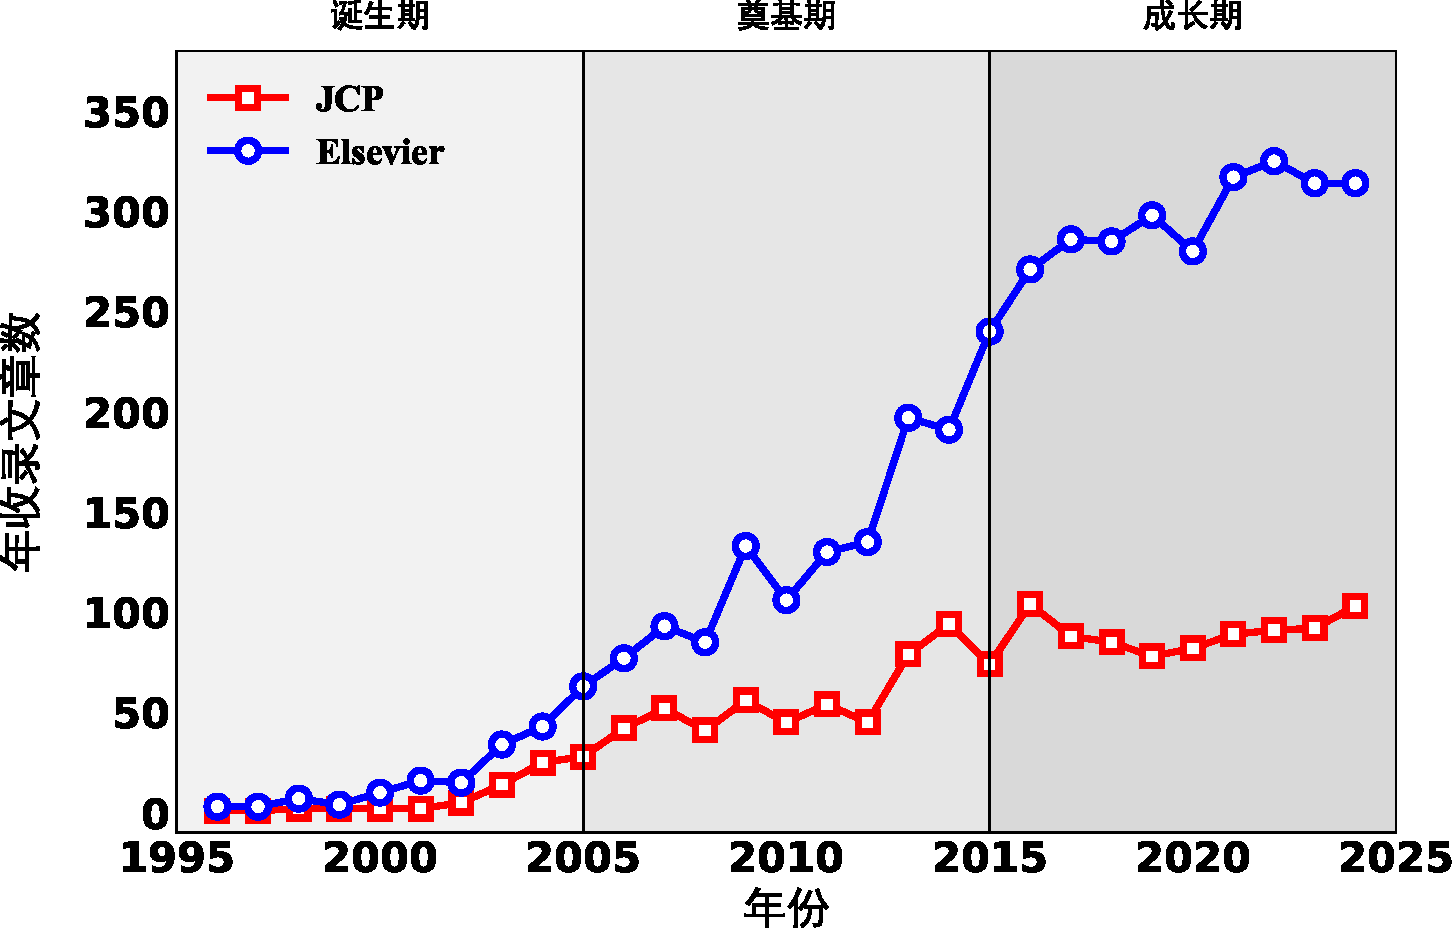
\includegraphics[width=0.7\linewidth]{figure/other/WENO_num.pdf}
    \caption{WENO格式相关论文发表数量（数据来源：Web of Science，检索条件：标题包含"WENO"且主题包含"numerical method"）。}
    \label{fig:weno-publications}
\end{figure}


WENO-JS格式在一阶极值点附近存在精度退化问题，其本质原因在于光滑度指标在极值点处丢失了高阶精度信息，导致非线性权重偏离最优线性权重的程度超出了应有的量级。为此先后提出了多种改进方案。Henrick等人~\cite{henrick2005mapped}通过对WENO-JS非线性权重施加映射函数，使得权重在光滑区域更接近最优线性权重，构造了WENO-M格式，在临界点处恢复了最优收敛阶，但引入了额外计算开销。Borges等人~\cite{borges2008improved}引入全局光滑度指标$\tau_5$（由局部光滑度指标的线性组合构造），提出了计算效率更高的WENOZ格式，以远小于WENO-M的计算量在一阶极值点处达到最优阶收敛，同时在冲击波捕捉和间断处理方面表现优异。Acker和Borges进一步指出WENOZ格式分辨率提升的主要原因在于欠光滑模板权重的增加，并在此基础上提出了WENOZ+格式~\cite{acker2016improved}，通过在非线性权重中添加新项以适当增加欠光滑模板的贡献，在高梯度光滑区获得了更高的分辨率。此后，多分辨率WENO（MRWENO）~\cite{ZHU2018659}通过嵌套的多分辨率分析构造非线性权重，在保持高阶精度的同时显著降低了数值耗散；截断ENO（TENO）~\cite{Fu2023ReviewOT}通过引入离散的模板选择机制替代连续的非线性加权，在间断附近实现了更为锐利的捕获，同时在光滑区域保持了高阶精度。这些格式各有侧重地在精度、耗散特性、鲁棒性等方面作出改进，推动了WENO格式在复杂流动模拟中的持续进步.


在两相流数值模拟的具体应用中，重构变量的选取对格式性能有重要影响。直接重构守恒变量$[\tilde{\rho}_1, \tilde{\rho}_2, \rho u, \rho v]^\top$虽然实现最为直接，但即使在压力和速度均匀的情形下也往往难以避免界面处的非物理压力振荡~\cite{li2020finite,coralic2014finite}。重构特征变量通过将守恒变量投影到特征空间后再实施WENO重构，能在保持高阶精度的同时有效抑制界面振荡，已由Zhang等人~\cite{zhang2023physical}在DG框架下得到严格的理论验证,但由于需要计算矩阵乘法，增加了额外的计算成本。重构原始变量是另一常用策略，有助于直接满足Abgrall原则，但重构变量集合仍是一个开放问题。直接重构相密度$\rho_k$虽然物理意义明确，但在界面处小体积分数导致的密度突变会引入显著的数值不稳定。


在两相流的三方程模型中，保持分相密度$\tilde{\rho}_k = z_k \rho_k > 0$至关重要。由特征分析可知，$\tilde{\rho}_k > 0$是控制方程双曲性的必要条件——一旦某一相分相密度变为负值，混合声速将失去实数意义，方程系统将丧失双曲性，数值求解将面临失稳乃至崩溃的风险。对于含大密度比和剧烈界面变形的问题（如溃坝流动中水-空气界面的剧烈破碎、Rayleigh--Taylor不稳定性中蘑菇状卷起结构的形成），分相密度的正性保持尤为困难，需要通过额外的限制算法加以保障。

早期研究发现，许多一阶Godunov型格式在适当CFL条件下具有内在的正性保持特性，部分二阶守恒格式在更严格的CFL限制下也能维持正性。然而高阶格式（包括WENO格式）通常不具备此类性质，其重构过程可能在极端情形下产生违反物理约束的界面状态。最简单的处理方法是将负值截断为小的正数，但这破坏了质量守恒性，在大多数实际问题中最终导致计算发散。

Zhang和Shu~\cite{zhang2011maximum}在这一领域取得了重要突破，提出了构造保极值或保正高阶数值方法的统一框架。其核心思想是通过凸分解，将单元平均更新方程表示为若干一维前向欧拉格式的凸组合，从而将高维问题的保正性分析归结为低维问题。在此基础上，通过对WENO重构所得到的界面状态施加如下缩放型限制器：令$\tilde{Q}_{i,j}(x,y) = \theta(Q_{i,j}(x,y) - \bar{Q}_{i,j}) + \bar{Q}_{i,j}$，其中缩放因子$\theta \in [0,1]$由界面状态的最小值与单元平均值之差确定，在适当CFL条件下可以严格保证界面状态属于物理可容许集，同时不影响格式的高阶精度。该限制器因实现简单、不破坏守恒性且对精度无负面影响，在计算流体力学中得到了广泛应用，并被推广至可压缩欧拉方程~\cite{zhang2011positivity}、可压缩多介质五方程模型~\cite{Zhang2025exponential}等一系列方程中，取得了良好的计算效果。

然而，将上述保正限制框架推广至基于非多项式逼近空间的高阶格式面临本质困难：传统凸分解分析的关键步骤依赖Gauss-Lobatto求积公式对重构多项式的精确积分，而对于$\tanh(\lambda x)$等非多项式基函数，这类精确积分一般不存在，需要采用数值积分近似，由此引入的误差可能破坏保正性的严格保证。张帆等人~\cite{Zhang2025exponential}针对指数多项式逼近空间发展了适配的保正限制算法，通过将非多项式重构解在积分点处进行修正，并结合对形状参数取值范围的约束，建立了非多项式WENO框架下的保正性理论，为本文在弱可压缩三方程模型中实现保正限制算法提供了重要的方法论基础。

综合以上分析，弱可压缩两相流高精度数值方法的发展已取得显著进展，但在以下方面仍存在研究缺口：其一，将指数多项式逼近空间WENO格式引入弱可压缩三方程模型的有限体积离散框架，针对该模型的特殊结构（无能量方程、等熵状态方程、瞬时压力平衡）设计适配的形状参数自适应策略，尚未有相关工作开展；其二，如何在非多项式逼近空间下同时实现Abgrall速度压力平衡性与分相密度正性保持的理论证明，仍是未解决的理论问题；其三，如何在提升精度的同时不引入额外的非物理振荡，在大密度比含间断问题中保持格式的鲁棒性，需要通过系统的数值算例加以验证。本文的工作正是针对上述三方面缺口展开的，旨在填补弱可压缩两相流高精度计算方法领域的上述空白。
\subsubsection{非多项式逼近空间 WENO 格式及其发展}

传统WENO格式基于多项式逼近空间，这一选择的主要优点是理论成熟、计算简便。然而，由于多项式逼近空间的平移和缩放不变性，其重构结果无法根据解的局部特性进行自适应调整，难以针对含大梯度或高振荡特征的区域进行有针对性的优化，导致数值耗散较为显著。为克服这一局限，基于非多项式逼近空间的WENO格式受到广泛关注，其核心思想是通过引入含可调参数（形状参数）的非多项式基函数，使逼近空间能够根据解的局部特性进行自适应调整。

在三角函数基函数方面，Zhu和Qiu~\cite{zhu2010trigonometric}提出了基于三角函数空间
\begin{equation}
    \mathrm{span}\{1, \sin(\alpha x), \cos(\alpha x), \sin((\alpha+1)x), \cos((\alpha+1)x)\}
\end{equation}
的五阶三角函数WENO（TWENO）格式，在含强激波的问题中表现出良好的鲁棒性，并将其进一步推广为间断有限元方法的限制器~\cite{zhu2013weno}，在高度振荡问题中相较于多项式方案展现出更优的性能。然而三角函数空间的参数选取较为敏感，且公式推导相对繁琐，限制了其推广应用。

在径向基函数方面，Guo 和 Jung~\cite{guo2017radial,GUO201727}提出了基于 RBF 非多项式空间的 ENO/WENO 格式，通过引入形状参数对插值进行调控，将非多项式插值表示为多项式插值的微扰形式，从而在不增加模板规模的情况下提升局部精度。为保证间断附近的无振荡性，该方法引入单调多项式插值作为切换机制，在非光滑区域退化为经典多项式重构。数值结果表明，该方法在光滑区域具有更高精度，并在间断附近呈现更锐利的解结构。然而，其性能对形状参数较为敏感，一定程度上增加了方法的复杂性。

在指数多项式基函数方面，近年来取得了一系列重要进展。Ha等人~\cite{Ha2016}采用基函数空间
\begin{equation}
    \mathrm{span}\{1, x, e^{\lambda x}, e^{-\lambda x}, \cos(\lambda x), \sin(\lambda x)\}
\end{equation}
提出了六点六阶WENO格式，将形状参数固定为$\lambda\Delta x = 1$，数值结果表明该方案能够清晰捕捉间断同时保持基本无振荡特性。然而固定形状参数的策略未能充分发挥非多项式插值的自适应优势，分辨率与精度提升有限。随后，Ha等人~\cite{Ha2021}通过将指数多项式表示为多项式的微扰，利用Taylor展开分析截断误差，推导出使高阶误差项消失的最优形状参数条件，在五点模板上实现了六阶收敛精度，相较于相同模板宽度的多项式WENO格式精度提升了一阶。这一工作的关键创新在于建立了形状参数与精度升阶条件之间的显式关系，使得形状参数可以根据解的局部高阶导数信息自适应优化，而非固定取值。其采用的函数空间为
\begin{equation}
    \mathrm{span}\{1, x, x^2, \sinh(\lambda x), \cosh(\lambda x)\},
\end{equation}
在形状参数趋近于零时自然退化为标准多项式WENO重构，保持了良好的渐近性质，Lee等人~\cite{Lee2023}进一步将此思路推广至三点四阶格式。上述指数多项式WENO格式的核心优势在于：通过引入可调形状参数，能够自适应提升精度，避免了三角函数WENO格式中固定参数和RBF-WENO格式中需要额外间断探测机制的缺陷。

张帆等人~\cite{Zhang2025exponential}将指数多项式逼近空间WENO格式首次应用于可压缩两介质流动的五方程模型，系统推导了形状参数的精度升阶条件与非负线性权重上界，并发展了适用于非多项式逼近空间的保正限制算法，通过严格的理论分析证明了保正性，取得了优于传统多项式WENO格式的数值表现。然而，目前的参数自适应策略主要基于局部高阶导数信息，尚未充分利用解的其他局部特征（如振荡指标、间断探测器等）来指导形状参数的调整，以进一步提升格式在含间断问题中的性能。此外，非多项式WENO插值在弱可压缩两相流动数值模拟中的性能仍尚未得到研究。


\subsection{本文的主要工作与内容安排}

本文针对弱可压缩不混溶两相流的高精度数值模拟问题，以三方程弱可压缩模型为控制方程，提出了一种基于指数多项式逼近空间的有限体积WENO格式，并配套建立了保正限制算法。本文的研究工作是在Li等人~\cite{li2020finite,li2022simplified}和Zhang等人~\cite{zhang2023physical,zhang2025positivity}所建立的弱可压缩两相流有限体积WENO框架与DG框架的基础上，将Ha等人~\cite{Ha2021}和张帆等人~\cite{Zhang2025exponential}所发展的指数多项式逼近空间WENO方法引入弱可压缩三方程模型，并在此基础上提出了一种新的形状参数自适应选取策略，以提升格式在含大梯度问题中的性能。针对该模型的特殊数学结构进行了系统的理论分析与算法设计。主要工作包括以下四个方面：
\begin{enumerate}
    \item \textbf{非多项式逼近空间的WENO重构格式。}针对弱可压缩三方程模型，构建了一种基于双曲正切函数的非多项式逼近空间有限体积WENO格式，其三点子模板上的函数空间定义为
    \begin{equation}
        \Omega_3 = \mathrm{span}\{1, \tanh(\lambda x), x^2\}
    \end{equation}
    可以通过调整自由参数 $\lambda$ 来改变逼近空间的局部特性。五阶函数函数空间采用
    \begin{equation}
        \Omega_5 = \mathrm{span}\{1, x, x^2, \tanh(\lambda x), x^4\},
    \end{equation}
    通过对大模板重构的截断误差进行Taylor展开分析，推导出使五阶误差项消失的最优形状参数条件，使高阶重构精度从五阶提升至六阶；在间断附近则通过一套新设计的自适应策略来调节形状参数，降低算法耗散。本文系统推导了算法的各项参数。
    \item \textbf{保正限制算法的设计与证明。} 针对非多项式逼近空间，本文提出并证明了一套完整的保正限制算法，确保分相密度$\tilde{\rho}_k > 0$（$k = 1, 2$）在整个计算过程中严格成立。上述理论结果将传统多项式格式保正分析框架成功推广至非多项式逼近空间，为指数多项式WENO格式在弱可压缩两相流中的可靠应用提供了严格的理论保障。
    \item \textbf{速度压力平衡性的理论证明。}本文从理论上系统证明了所提算法的每个部分均满足Abgrall原则~\cite{ABGRALL1996150}，即在孤立相界面对流过程中能够严格保持均匀压力与速度剖面。具体地，本文分别针对以下四个方面给出了完整的速度压力平衡证明：
    \begin{itemize}
        \item 有限体积法离散格式本身
        \item 近似黎曼求解器
        \item WENO重构
        \item 保正限制器
    \end{itemize}
    
    \item \textbf{系统数值验证。} 通过一系列标准算例，从精度、界面捕获能力及鲁棒性等方面对所提格式进行了系统验证。数值结果表明，该格式在光滑问题中能够达到预期的高阶收敛精度，在多维情形下依然保持良好的收敛性；在界面问题中具有无振荡且界面锐利的重构能力，相比传统WENO-JS格式能够有效减小界面过渡区宽度；在自由液面流动模拟中表现出较低的数值耗散和良好的长时间积分精度；此外，在大密度比和剧烈界面变形条件下仍具有良好的计算稳定性，其中保正限制器对于保证数值计算的成功至关重要。  
\end{enumerate}



本文共分五章。第一章为绪论，介绍研究背景，综述两相流问题的高精度数值模拟方法的研究现状。第二章建立弱可压缩两相流的三方程数学模型，以及传统高精度数值格式在三方程中的应用。第三章推导非多项式WENO逼近空间的理论框架，给出WENO-EXP格式的具体构造方案及其对应的自由参数自适应策略。第四章给出系统的数值验证结果，通过多类算例全面考察所提格式的精度、界面捕获能力与鲁棒性。第五章对全文工作进行总结并展望未来研究方向。



% \begin{figure}[!htbp]
%     \centering
%     \resizebox{\textwidth}{!}{%
%         \begin{tikzpicture}[
    font=\sffamily\small,
    >=Stealth,
    arr/.style   = {->,  draw=gray!70, line width=1.2pt},
    biarr/.style = {<->, draw=gray!70, line width=1.2pt},
    titlebox/.style = {
      rectangle, rounded corners=3pt,
      draw=cBlue, line width=1.6pt, fill=cTitle,
      minimum width=12cm, minimum height=0.85cm,
      text centered, text width=11.8cm
    },
    probbox/.style = {
      rectangle, rounded corners=3pt,
      draw=cBlue!80, line width=1pt, fill=cProb,
      minimum width=3.2cm, minimum height=0.82cm,
      text centered, text width=3.0cm
    },
    methbox/.style = {
      rectangle, rounded corners=3pt,
      draw=cOrange, line width=1pt, fill=cMeth,
      minimum width=2.9cm, minimum height=0.72cm,
      text centered
    },
    labelbox/.style = {
      rectangle, rounded corners=2pt,
      draw=gray!60, line width=0.8pt, fill=cLabel,
      minimum width=1.3cm, minimum height=0.7cm,
      text centered, font=\footnotesize\sffamily
    },
  ]
   
  % ── 研究目标 ────────────────────────────────────────────────
  \node[titlebox] (title) at (0,0)
    {弱可压缩不混溶两相流高精度数值模拟方法研究};
  \node[labelbox, left=5mm of title] {研究\\目标};
   
  % ── 科学问题 ────────────────────────────────────────────────
  \node[probbox, below left=1.0cm and 4.1cm of title]  (p1)
    {非物理压力振荡\\（Abgrall 原则）};
  \node[probbox, below=1.0cm of title]                  (p2)
    {分相密度正性保持\\（双曲性条件）};
  \node[probbox, below right=1.0cm and 4.1cm of title] (p3)
    {数值耗散与\\相界面弥散};
  \node[labelbox, left=5mm of p1] {科学\\问题};
   
  \draw[arr] (title.south) -- (p1.north);
  \draw[arr] (title.south) -- (p2.north);
  \draw[arr] (title.south) -- (p3.north);
   
  % ── 研究方法 ────────────────────────────────────────────────
  \node[methbox, below=0.9cm of p1] (m1) {理论分析};
  \node[methbox, below=0.9cm of p2] (m2) {互相验证};
  \node[methbox, below=0.9cm of p3] (m3) {数值实验};
  \node[labelbox, left=5mm of m1]   {研究\\方法};
   
  \draw[arr]   (p1) -- (m1);
  \draw[arr]   (p2) -- (m2);
  \draw[arr]   (p3) -- (m3);
  \draw[biarr] (m1) -- (m2);
  \draw[biarr] (m2) -- (m3);
   
  \end{tikzpicture}
%     }
%     \caption{论文框架图}
%     \label{fig:outline}
% \end{figure}


\cleardoublepage
\section{使用WENO有限体积法求解三方程模型}

\subsection{三方程模型与离散格式}
% \paragraph{弱可压缩两相流的三方程模型}
本文采用三方程模型~\cite{Chanteperdrix2004,grenier2013accurate}描述弱可压缩无粘两相流体的流动行为。该模型由两相各自的质量守恒方程与混合物的动量守恒方程组成，控制方程组具有如下的形式：
\begin{equation}
    \label{eq:governing}
    \frac{\partial \bm{Q}}{\partial t} + \nabla \cdot \bm{F}(\bm{Q}) = \bm{S},
\end{equation}
其中守恒变量向量 $\bm{Q}$、通量张量 $\bm{F}(\bm{Q})$ 及源项向量 $\bm{S}$ 分别定义为
\begin{equation}
    \bm{Q} =
    \begin{bmatrix}
        \tilde{\rho}_1 \\
        \tilde{\rho}_2 \\
        \rho \bm{u}
    \end{bmatrix},
    \qquad
    \bm{F}(\bm{Q}) =
    \begin{bmatrix}
        \tilde{\rho}_1 \bm{u} \\
        \tilde{\rho}_2 \bm{u} \\
        \rho \bm{u} \otimes \bm{u} + p \bm{I}
    \end{bmatrix},
    \qquad
    \bm{S} = \begin{bmatrix}
        0 \\
        0 \\
        \rho \bm{g}
    \end{bmatrix},
\end{equation}
其中 $\bm{I}$ 为单位张量，$\otimes$ 表示张量积，$\bm{u} = (u, v)^\top$
为两相共享的混合物速度，$\bm{g} = (g_x, g_y)^\top$ 为体积力加速度向量。
在仅受重力作用的情形下，取 $g_x = 0$，$g_y = -g$，$g$ 为重力加速度大小。

上述方程中，$\tilde{\rho}_k(\bm{x}, t) = z_k(\bm{x}, t)\,\rho_k(\bm{x}, t)$
为第 $k$ 相（$k = 1, 2$）的分相密度，$z_k(\bm{x}, t)$ 与
$\rho_k(\bm{x}, t)$ 分别为其体积分数与相密度，且满足约束条件
$z_1(\bm{x}, t) + z_2(\bm{x}, t) = 1$。混合物密度与混合物压力由
混合规则给出：
\begin{equation}
    \rho(\bm{x}, t) = \sum_{k=1}^{2} z_k \rho_k, \qquad
    p(\bm{x}, t)   = \sum_{k=1}^{2} z_k p_k,
\end{equation}
其中 $p_k(\bm{x}, t)$ 为第 $k$ 相的单相压力。此外，本文采用瞬时压力平衡假设，即两相单相压力在计算域内任意位置和时刻均满足
\begin{equation}
    p(\bm{x}, t) = p_1(\bm{x}, t) = p_2(\bm{x}, t),
    \quad \forall\, \bm{x} \in \Omega_f,\ \forall\, t \in [0, +\infty).
\end{equation}
正如 Drew~\cite{drew1982mathematical} 所指出，当声速远大于流场特征速度、即马赫数足够小时，该假设具有充分的物理合理性，与弱可压缩流动的情形相符。%基于上述假设，本文所采用的控制方程系统属于``单压力—单速度''两相模型~\cite{stewart1984two}。
% \paragraph{等熵闭合关系}
% 单相压力 $p_k$ 通过状态方程与各相密度 $\rho_k$ 相关联。
参照文献~\cite{grenier2013accurate}，本文采用如下等熵状态方程对控制方程组~\eqref{eq:governing}进行封闭：
\begin{equation}
    \label{eq:eos_single}
    p_k = p_0 + c_k^2 \left(\rho_k - \rho_{k,0}\right), \quad k = 1, 2,
\end{equation}
其中 $p_0$、$\rho_{k,0}$ 与 $c_k$ 均为常数，分别表示参考压力、
第 $k$ 相的参考密度与声速。由于本文不考虑热效应，控制方程组
中不含能量方程，因此等熵状态方程~\eqref{eq:eos_single}的
采用是合理的。

%值得指出的是，在等熵闭合关系~\eqref{eq:eos_single}下，所采用的三方程两相模型构成双曲型系统，其雅可比矩阵的特征值均为实数，与流体域内信息的传播速度（即声速）相对应，详见第~\autoref{sec:characteristic}节的特征分析。

\begin{remark}
当压力恢复至参考值 $p_k = p_0$ 时，由式~\eqref{eq:eos_single}
可知各相密度相应地恢复至参考密度，即 $\rho_k = \rho_{k,0}$。
\end{remark}

\begin{remark}
在数值计算中，相密度 $\rho_k$ 由 $\rho_k = \tilde{\rho}_k / z_k$
计算得到。当某一相的体积分数 $z_k$ 趋近于零时，该比值将产生
较大的数值误差。为避免此类情形，实际计算中可采用如下策略确定混合物压力：
\begin{equation}
    p = \begin{cases}
        p_1, & z_1 \geqslant z_2, \\
        p_2, & z_1 < z_2.
    \end{cases}
\end{equation}
即优先采用体积分数较大相的单相压力作为混合物压力，从而避免
因小体积分数导致的数值不稳定问题。
\end{remark}
% \paragraph{两相混合物中的声速}

% 在当前弱可压缩两相模型框架下，两相混合物的声速 $c(\bm{x}, t)$
% 由 Wood 公式给出：
% \begin{equation}
%     \label{eq:wood}
%     c = \left( \rho \left( \frac{z_1}{\rho_1 c_1^2}
%         + \frac{z_2}{\rho_2 c_2^2} \right) \right)^{-\frac{1}{2}},
% \end{equation}
% 其推导过程详见附录~A。以水-空气混合物为例，图~1 给出了混合声速随水相体积分数 $z_1$ 从~0 变化至~1 的演化规律。由图可知，当$z_1$ 接近~0.5 时，混合物局部声速可能远小于两相各自的声速$c_1$ 与 $c_2$。这一现象在其他多相模型中亦有类似报道~\cite{le2014towards,murrone2005five,saurel2016general,stewart1984two}，并已由 Costigan 和 Whalley~\cite{costigan1997measurements}在水-空气流动声速的实验测量中得到验证。
% \paragraph{平衡体积分数}

由控制方程组~\eqref{eq:governing}可知，方程组中不包含关于体积分数场 $z_k(\bm{x}, t)$ 的独立对流方程，即无需额外方程显式更新体积分数。如文献~\cite{grenier2013accurate}所述，在已知分相密度 $\tilde{\rho}_1$ 与 $\tilde{\rho}_2$ 的条件下，体积分数 $z_1$ 可通过求解以下压力平衡方程隐式确定：
\begin{equation}
    \label{eq:EOS}
    p_0 + c_1^2 \left( \frac{\tilde{\rho}_1}{z_1} - \rho_{1,0} \right)
    = p_0 + c_2^2 \left( \frac{\tilde{\rho}_2}{1 - z_1} - \rho_{2,0} \right).
\end{equation}
一旦求得 $z_1$，第二相的体积分数随即由 $z_2 = 1 - z_1$ 给出。可以证明，当 $\tilde{\rho}_1 > 0$ 且 $\tilde{\rho}_2 > 0$ 时，方程~\eqref{eq:EOS}存在唯一满足 $0 < z_1 < 1$ 的有效解。为便于求解，参照文献~\cite{Chanteperdrix2004}，令 
\begin{equation}
    \gamma = z_1 / (1 - z_1), q = \rho_{2,0} c_2^2 - \rho_{1,0} c_1^2,\tilde{q} = \tilde{\rho}_2 c_2^2 - \tilde{\rho}_1 c_1^2
\end{equation}
则方程~\eqref{eq:EOS}等价于如下二次方程：
\begin{equation}
    \label{eq:quadratic}
    \tilde{\rho}_2 c_2^2\, \gamma^2 - (q - \tilde{q})\,\gamma
    - \tilde{\rho}_1 c_1^2 = 0.
\end{equation}
当 $\tilde{\rho}_1 > 0$ 且 $\tilde{\rho}_2 > 0$ 时，
方程~\eqref{eq:quadratic}有两个实数根：
\begin{equation}
    \begin{aligned}
        \gamma^+ & = \frac{(q - \tilde{q})
            + \sqrt{(q - \tilde{q})^2 + 4\tilde{\rho}_2 c_2^2\,\tilde{\rho}_1 c_1^2}}
            {2\tilde{\rho}_2 c_2^2} > 0, \\[4pt]
        \gamma^- & = \frac{(q - \tilde{q})
            - \sqrt{(q - \tilde{q})^2 + 4\tilde{\rho}_2 c_2^2\,\tilde{\rho}_1 c_1^2}}
            {2\tilde{\rho}_2 c_2^2} < 0.
    \end{aligned}
\end{equation}
由于 $z_1$ 须满足 $0 < z_1 < 1$，即 $\gamma > 0$，故 $\gamma^+$
为唯一有效解，对应的平衡体积分数为：
\begin{equation}
    z_1 = \frac{\gamma^+}{1 + \gamma^+}.
\end{equation}

% \begin{remark}
% 由方程~\eqref{eq:EOS}解的唯一性可知，若在数值计算中能够找到某一满足方程~\eqref{eq:EOS}的解 $(z_k)_i$，则该解必为方程~\eqref{eq:EOS}的唯一平衡解。
% \end{remark}
% \paragraph{特征分析}
% \label{sec:characteristic}

对控制方程组~\eqref{eq:governing}沿任意法方向 $\bm{n}_e = (n_x, n_y)^\top$
进行特征分析，其对应的雅可比矩阵为~\cite{zhang2023physical}
\begin{equation}
    \label{eq:jacobian}
    \bm{J}
    = \frac{\partial \bigl(\bm{n}_e \cdot \bm{F}(\bm{Q})\bigr)}{\partial \bm{Q}}
    =
    \begin{bmatrix}
        \dfrac{\tilde{\rho}_2}{\rho} u_n
         & -\dfrac{\tilde{\rho}_1}{\rho} u_n
         &  \dfrac{\tilde{\rho}_1}{\rho} n_x
         &  \dfrac{\tilde{\rho}_1}{\rho} n_y \\[3mm]
        -\dfrac{\tilde{\rho}_2}{\rho} u_n
         &  \dfrac{\tilde{\rho}_1}{\rho} u_n
         &  \dfrac{\tilde{\rho}_2}{\rho} n_x
         &  \dfrac{\tilde{\rho}_2}{\rho} n_y \\[3mm]
        \tilde{c}_1^2 n_x - u\, u_n
         & \tilde{c}_2^2 n_x - u\, u_n
         & u_n + u\, n_x
         & u\, n_y \\[3mm]
        \tilde{c}_1^2 n_y - v\, u_n
         & \tilde{c}_2^2 n_y - v\, u_n
         & v\, n_x
         & u_n + v\, n_y
    \end{bmatrix},
\end{equation}
其中 $u_n = \bm{u} \cdot \bm{n}_e$ 为法向速度，
$\tilde{c}_k^2 = \partial p / \partial \tilde{\rho}_k$
为分相等效声速平方，具体表达式为
\begin{equation}
    \label{eq:phase_sound_speed}
    \tilde{c}_1^2
    = \frac{c_1^2}{z_1}
    \cdot\frac{c_2^2 \tilde{\rho}_2 / z_2^2}
    {c_1^2 \tilde{\rho}_1 / z_1^2 + c_2^2 \tilde{\rho}_2 / z_2^2},
    \qquad
    \tilde{c}_2^2
    = \frac{c_2^2}{z_2}
    \cdot\frac{c_1^2 \tilde{\rho}_1 / z_1^2}
    {c_1^2 \tilde{\rho}_1 / z_1^2 + c_2^2 \tilde{\rho}_2 / z_2^2}.
\end{equation}
雅可比矩阵~\eqref{eq:jacobian}具有四个特征值：
\begin{equation}
    \label{eq:eigenvalues}
    \lambda_1 = u_n - c,
    \qquad
    \lambda_2 = \lambda_3 = u_n,
    \qquad
    \lambda_4 = u_n + c,
\end{equation}
其中混合声速 $c$ 由 Wood 公式给出：
\begin{equation}
    \label{eq:wood2}
    \frac{1}{\rho c^2}
    = \frac{z_1}{\rho_1 c_1^2} + \frac{z_2}{\rho_2 c_2^2}.
\end{equation}
该表达式等价于
\begin{equation}
    \label{eq:wood_tilde}
    \rho c^2 = \tilde{\rho}_1 \tilde{c}_1^2 + \tilde{\rho}_2 \tilde{c}_2^2.
\end{equation}

由此可知，混合声速 $c$ 为实数的充要条件是分相密度 $\tilde{\rho}_1$ 与$\tilde{\rho}_2$ 均严格为正。由此可得如下引理。

\begin{lemma}
    对于弱可压缩两相流控制方程组~\eqref{eq:governing}，当
\begin{equation}
    \tilde{\rho}_1 > 0 \quad \text{且} \quad \tilde{\rho}_2 > 0
\end{equation}
时，雅可比矩阵~\eqref{eq:jacobian}的所有特征值均为实数，从而控制方程系统保持双曲性。
\end{lemma}


进一步地，雅可比矩阵~\eqref{eq:jacobian}的右特征矩阵
$\bm{R}(\bm{Q})$ 与左特征矩阵 $\bm{L}(\bm{Q})$ 分别为\textcolor{red}{
\begin{equation}
    \bm{R}(\bm{Q}) =
    \begin{bmatrix}
        \dfrac{\tilde{\rho}_1}{\rho}
         & -\dfrac{\cos\theta\,\tilde{c}_2^2}{\tilde{c}_1^2 - \tilde{c}_2^2}
         & -\dfrac{\sin\theta\,\tilde{c}_2^2}{\tilde{c}_1^2 - \tilde{c}_2^2}
         & \dfrac{\tilde{\rho}_1 v}{\rho(v + c\sin\theta)} \\[3mm]
        \dfrac{\tilde{\rho}_2}{\rho}
         & \dfrac{\cos\theta\,\tilde{c}_1^2}{\tilde{c}_1^2 - \tilde{c}_2^2}
         & \dfrac{\sin\theta\,\tilde{c}_1^2}{\tilde{c}_1^2 - \tilde{c}_2^2}
         & \dfrac{\tilde{\rho}_2 v}{\rho(v + c\sin\theta)} \\[3mm]
        u - c\cos\theta & u_n & 0
         & \dfrac{v(u + c\cos\theta)}{v + c\sin\theta} \\[3mm]
        v - c\sin\theta & 0 & u_n & v
    \end{bmatrix},
\end{equation}
\begin{equation}
    \bm{L}(\bm{Q}) =
    \begin{bmatrix}
        \dfrac{c u_n + \tilde{c}_1^2}{2c^2}
         & \dfrac{c u_n + \tilde{c}_2^2}{2c^2}
         & -\dfrac{\cos\theta}{2c}
         & -\dfrac{\sin\theta}{2c} \\[3mm]
        \sin\theta - \dfrac{\tilde{c}_1^2 v}{c^2 u_n}
         & \sin\theta - \dfrac{\tilde{c}_2^2 v}{c^2 u_n}
         & -\dfrac{\sin 2\theta}{2 u_n}
         & \dfrac{\cos^2\theta}{u_n} \\[3mm]
        \cos\theta - \dfrac{\tilde{c}_1^2 u}{c^2 u_n}
         & \cos\theta - \dfrac{\tilde{c}_2^2 u}{c^2 u_n}
         & \dfrac{\sin^2\theta}{u_n}
         & -\dfrac{\sin 2\theta}{2 u_n} \\[3mm]
        \dfrac{(\tilde{c}_1^2 - c u_n)(v + c\sin\theta)}{2c^2 v}
         & \dfrac{(\tilde{c}_2^2 - c u_n)(v + c\sin\theta)}{2c^2 v}
         & \dfrac{\sin 2\theta}{4v} + \dfrac{\cos\theta}{2c}
         & \dfrac{\sin\theta}{2c} + \dfrac{\sin^2\theta}{2v}
    \end{bmatrix},
\end{equation}
}
其中 $\theta$ 为法向角，满足 $n_x = \cos\theta$，$n_y = \sin\theta$，
且 $\bm{L}(\bm{Q}) = \bm{R}^{-1}(\bm{Q})$。
% \subsubsection{数值求解的主要难点}

% 弱可压缩两相流的数值求解面临以下几方面核心挑战，
% 是格式设计时需重点关注的问题。

% \paragraph{（一）速度压力平衡性与 Abgrall 原则}
% 当流场处于均匀压力 $p \equiv p_0$、均匀速度
% $\bm{u} \equiv \bm{u}_0$ 的平衡状态时，即使存在密度或体积分数梯度
% （即相界面），数值格式亦应在离散水平上精确维持该状态，即要求：
% 若 $p^n \equiv p_0$ 且 $\bm{u}^n \equiv \bm{u}_0$，
% 则 $p^{n+1} \equiv p_0$ 且 $\bm{u}^{n+1} \equiv \bm{u}_0$，
% 对计算域内所有单元成立。
% 若格式不满足此条件，将在相界面附近产生非物理的压力振荡与速度扰动，
% 即所谓"寄生振荡"（parasitic oscillations）或伪速度场
% （spurious currents）~\cite{}。满足上述条件（即 Abgrall 原则~\cite{}）
% 是避免界面处数值污染的关键。

% \paragraph{（二）物理量的正性保持}
% 在计算过程中，两相分相密度 $\tilde{\rho}_k = z_k \rho_k$ 须在
% 任意时刻严格保持正值，进而保证体积分数 $z_k \in (0,1)$
% 与相密度 $\rho_k > 0$ 的物理有界性。由引理~1 可知，
% $\tilde{\rho}_k > 0$ 是保证控制方程双曲性的必要条件，
% 一旦该条件被破坏，混合声速将失去实数意义，数值求解
% 将面临失稳乃至崩溃的风险。因此，格式须通过适当的
% 限制器或受限时间步长（CFL 条件）等手段，在每一时间步
% 内显式地维持 $\tilde{\rho}_k > 0$。

% \paragraph{（三）质量守恒性}
% 质量守恒是两相流数值模拟的基本物理约束。控制方程组
% ~\eqref{eq:governing}的前两个分量方程为两相的质量守恒方程，
% 在无源项的情形下，各相质量在计算域上满足精确守恒。
% 然而，若数值格式不具备严格的守恒性，则在界面对流过程中
% 各相质量将产生数值漂移，导致密度分布失真，进而影响界面
% 位置与流场结构的准确性。因此，数值格式须采用守恒型离散
% 形式，以确保两相质量在离散水平上的精确守恒，这对于长时间
% 积分或含强界面变形的流动问题尤为重要。

% \paragraph{（四）界面清晰度与数值耗散}
% 本文采用界面捕获（interface capturing）策略，体积分数
% $z_k$ 作为连续场量在全计算域内演化。由于缺乏显式的
% 界面重构步骤，数值耗散将导致界面区域逐渐弥散，
% 使相界面厚度增加、位置模糊，进而降低界面相关物理机制
% 的预测精度。高阶数值格式（如 WENO 重构或不连续 Galerkin 方法）
% 的采用正是为了在维持格式稳定性的同时，尽量抑制数值耗散，
% 实现对相界面的清晰捕获。

% \paragraph{（五）时间步长限制}
% 在弱可压缩模型中，声速 $c_k$ 通常远大于流场特征速度，
% 由此导致显式时间推进格式受到严格的 CFL 条件约束：
% $\Delta t \leqslant \mathrm{CFL} \cdot \Delta x / (c + |\bm{u}|)$。
% 对于大密度比、大声速比或需要长时间积分的问题，
% 过小的时间步长将带来显著的计算代价。
% \cleardoublepage

% \subsubsection{模型离散化}
将计算域 $\Omega$ 划分为均匀矩形单元 $I_{i,j} = [x_{i-1/2},\, x_{i+1/2}]
\times [y_{j-1/2},\, y_{j+1/2}]$，网格间距恒定，记为
$\Delta x = x_{i+1/2} - x_{i-1/2}$，$\Delta y = y_{j+1/2} - y_{j-1/2}$。

对控制方程~\eqref{eq:governing}（忽略源项）在单元 $I_{i,j}$ 上积分，
并对面积归一化，得到守恒变量单元平均值的演化方程：
\begin{equation}
    \frac{\dd}{\dd t}\,\overline{\bm{Q}}_{i,j}
    = -\frac{1}{\Delta x \Delta y}
    \int_{\partial I_{i,j}} \bm{F}(\bm{Q}) \cdot \bm{n}\,\dd s,
\end{equation}
也即
\begin{equation}
    \label{eq:fv_boundary_integral}
    \begin{aligned}
        \frac{\dd}{\dd t}\overline{\bm{Q}}_{i,j}
        ={}&
        -\frac{1}{\Delta x\Delta y}
        \int_{y_{j-1/2}}^{y_{j+1/2}}
        \left[
        \hat{\bm{F}}_x\!\left(
        \bm{Q}_{i+1/2,j}^-,\bm{Q}_{i+1/2,j}^+
        \right)
        -
        \hat{\bm{F}}_x\!\left(
        \bm{Q}_{i-1/2,j}^-,\bm{Q}_{i-1/2,j}^+
        \right)
        \right]\dd y \\
        &-
        \frac{1}{\Delta x\Delta y}
        \int_{x_{i-1/2}}^{x_{i+1/2}}
        \left[
        \hat{\bm{F}}_y\!\left(
        \bm{Q}_{i,j+1/2}^-,\bm{Q}_{i,j+1/2}^+
        \right)
        -
        \hat{\bm{F}}_y\!\left(
        \bm{Q}_{i,j-1/2}^-,\bm{Q}_{i,j-1/2}^+
        \right)
        \right]\dd x,
    \end{aligned}
\end{equation}
其中
\begin{equation}
    \overline{\bm{Q}}_{i,j}^n
    = \frac{1}{\Delta x \Delta y}
    \int_{y_{j-1/2}}^{y_{j+1/2}} \int_{x_{i-1/2}}^{x_{i+1/2}}
    \bm{Q}(x, y, t^n)\,\dd x\,\dd y
\end{equation}
为时间层 $t^n$ 上守恒变量 $\bm{Q}$ 在单元 $I_{i,j}$ 上的平均值。展开边界积分，得到半离散有限体积格式：
\begin{equation}
    \label{eq:fv}
    \begin{aligned}
        \frac{\dd}{\dd t}\overline{\bm{Q}}_{i,j}
        = & -\frac{1}{\Delta x}
        \sum_{\beta=1}^{L} \eta_\beta
        \left[
            \hat{\bm{F}}_x\!\left(\bm{Q}_{i+1/2,\beta}^-,\, \bm{Q}_{i+1/2,\beta}^+\right)
            - \hat{\bm{F}}_x\!\left(\bm{Q}_{i-1/2,\beta}^-,\, \bm{Q}_{i-1/2,\beta}^+\right)
        \right] \\
          & -\frac{1}{\Delta y}
        \sum_{\beta=1}^{L} \eta_\beta
        \left[
            \hat{\bm{F}}_y\!\left(\bm{Q}_{\beta,j+1/2}^-,\, \bm{Q}_{\beta,j+1/2}^+\right)
            - \hat{\bm{F}}_y\!\left(\bm{Q}_{\beta,j-1/2}^-,\, \bm{Q}_{\beta,j-1/2}^+\right)
        \right],
    \end{aligned}
\end{equation}
其中单元边界上的积分已通过 $L$ 点 Lobatto--Gauss 求积公式近似，\textcolor{red}{
$\eta_\beta$ 为对应的求积权系数。$\bm{Q}_{i+1/2,\beta}^-$ 与
$\bm{Q}_{i+1/2,\beta}^+$ 分别为通过 WENO 重构得到的界面左、右侧重构值，
$\hat{\bm{F}}_x$、$\hat{\bm{F}}_y$ 为近似 Riemann 数值通量，
将在第~\autoref{sec:riemann}节中详细介绍。}

时间离散采用三阶强稳定保持 Runge--Kutta（SSP-RK3）格式~\cite{gottlieb2001strong}：
\begin{equation}
    \label{eq:ssprk}
    \begin{aligned}
        \overline{\bm{Q}}^{(1)}   & = \overline{\bm{Q}}^n
        + \Delta t^n\, \mathcal{L}(\overline{\bm{Q}}^n),                                                                   \\
        \overline{\bm{Q}}^{(2)}   & = \frac{3}{4}\,\overline{\bm{Q}}^n
        + \frac{1}{4}\,\overline{\bm{Q}}^{(1)}
        + \frac{1}{4}\,\Delta t^n\, \mathcal{L}(\overline{\bm{Q}}^{(1)}),                                                  \\
        \overline{\bm{Q}}^{n+1}   & = \frac{1}{3}\,\overline{\bm{Q}}^n
        + \frac{2}{3}\,\overline{\bm{Q}}^{(2)}
        + \frac{2}{3}\,\Delta t^n\, \mathcal{L}(\overline{\bm{Q}}^{(2)}),
    \end{aligned}
\end{equation}
其中 $\Delta t^n = t^{n+1} - t^n$ 为时间步长，$\mathcal{L}(\cdot)$ 表示式~\eqref{eq:fv}所定义的空间离散算子。时间步长由如下 CFL 条件确定：
\begin{equation}
    \label{eq:cfl}
    \Delta t^n \leqslant \mathrm{CFL} \cdot
    \min_{i,j} \left(
    \frac{\Delta x}{|u_{i,j}| + c_{i,j}},\;
    \frac{\Delta y}{|v_{i,j}| + c_{i,j}}
    \right),
\end{equation}
其中 $c_{i,j}$ 为单元 $I_{i,j}$ 中的混合声速。

\begin{remark}
    保正限制器的施加通常对时间步长有额外约束，且往往比 CFL 条件~\eqref{eq:cfl}更为严格，详见\autoref{sec:pplimiter}。
\end{remark}

由于 SSP-RK3 格式可以表示为前向 Euler 方法的凸组合，在分析和证明 $t^{n+1}$ 时刻数值解的相关性质时，只需对前向 Euler 时间离散进行分析即可。采用前向 Euler 时间离散的有限体积格式可显式地表示为：
\begin{equation}
    \label{eq:fv_euler}
    \begin{aligned}
        \overline{\bm{Q}}_{i,j}^{n+1}
        = \overline{\bm{Q}}_{i,j}^n
         & - \frac{\Delta t^n}{\Delta x} \sum_{\beta=1}^{L} \eta_{\beta}
        \left[
            \hat{\bm{F}}_x\!\left(\bm{Q}_{i+1/2,\beta}^-,\, \bm{Q}_{i+1/2,\beta}^+\right)
            - \hat{\bm{F}}_x\!\left(\bm{Q}_{i-1/2,\beta}^-,\, \bm{Q}_{i-1/2,\beta}^+\right)
        \right]  \\
         & - \frac{\Delta t^n}{\Delta y} \sum_{\beta=1}^{L} \eta_{\beta}
        \left[
            \hat{\bm{F}}_y\!\left(\bm{Q}_{\beta,j+1/2}^-,\, \bm{Q}_{\beta,j+1/2}^+\right)
            - \hat{\bm{F}}_y\!\left(\bm{Q}_{\beta,j-1/2}^-,\, \bm{Q}_{\beta,j-1/2}^+\right)
        \right].
    \end{aligned}
\end{equation}

\begin{figure}[!htbp]
    \centering
    \begin{subfigure}[b]{0.45\linewidth}
        \centering
                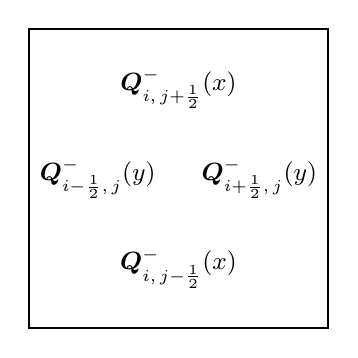
\begin{tikzpicture}[font=\small]
            \def\L{3.8}
    
            % Cell boundary
            \draw[line width=0.9pt] (0,0) rectangle (\L,\L);
    
            % % Corner coordinate labels (outside the cell)
            % \node[anchor=south east] at (0,\L)
            %     {\footnotesize$(x_{i-\frac{1}{2}},\,y_{j+\frac{1}{2}})$};
            % \node[anchor=south west] at (\L,\L)
            %     {\footnotesize$(x_{i+\frac{1}{2}},\,y_{j+\frac{1}{2}})$};
            % \node[anchor=north east] at (0,0)
            %     {\footnotesize$(x_{i-\frac{1}{2}},\,y_{j-\frac{1}{2}})$};
            % \node[anchor=north west] at (\L,0)
            %     {\footnotesize$(x_{i+\frac{1}{2}},\,y_{j-\frac{1}{2}})$};
    
            % Trace labels inside the cell
            \node at (0.50*\L, 0.80*\L)
                {$\bm{Q}^-_{i,\,j+\frac{1}{2}}(x)$};
            \node at (0.50*\L, 0.20*\L)
                {$\bm{Q}^-_{i,\,j-\frac{1}{2}}(x)$};
            \node at (0.23*\L, 0.50*\L)
                {$\bm{Q}^-_{i-\frac{1}{2},\,j}(y)$};
            \node at (0.77*\L, 0.50*\L)
                {$\bm{Q}^-_{i+\frac{1}{2},\,j}(y)$};
        \end{tikzpicture}
        \caption{traces of $\bm{Q}_h$}
        \label{fig:cell-traces}
    \end{subfigure}
    \hfill
    \begin{subfigure}[b]{0.45\linewidth}
        \centering
        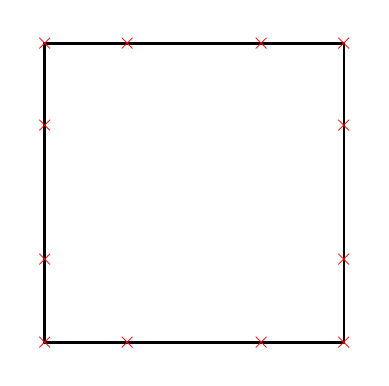
\begin{tikzpicture}
    \def\L{3.8}
    % 4-point Gauss--Lobatto positions in [0,1]:
    % (lambda+1)/2 for lambda in {-1, -0.4472, 0.4472, 1}
    \def\pa{0}
    \def\pb{0.2764}
    \def\pc{0.7236}
    \def\pd{1}

    % Cell boundary
    \draw[line width=0.9pt] (0,0) rectangle (\L,\L);

    % Bottom edge (y = 0): all 4 GL points
    \foreach \xi in {\pa, \pb, \pc, \pd}{
        \node[red, scale=0.85] at (\xi*\L, 0) {$\times$};
    }
    % Top edge (y = L): all 4 GL points
    \foreach \xi in {\pa, \pb, \pc, \pd}{
        \node[red, scale=0.85] at (\xi*\L, \L) {$\times$};
    }
    % Left edge (x = 0): interior 2 points only (corners already marked)
    \foreach \eta in {\pb, \pc}{
        \node[red, scale=0.85] at (0, \eta*\L) {$\times$};
    }
    % Right edge (x = L): interior 2 points only
    \foreach \eta in {\pb, \pc}{
        \node[red, scale=0.85] at (\L, \eta*\L) {$\times$};
    }
\end{tikzpicture}
        \caption{points set $S_{i,j}$}
        \label{fig:cell-points}
    \end{subfigure}
    \caption{\textcolor{red}{单元 $I_{i,j}$ 上的迹函数分布与求积点集 $S_{i,j}$。
             （a）四条边上的迹函数，其中水平边上的迹为 $x$ 的函数，
             竖直边上的迹为 $y$ 的函数；
             （b）保正限制器所需的求积点集 $S_{i,j}$，
             由三点 Gauss--Lobatto 公式在各边及角点处确定，共 $9$ 个积分点。}}
    \label{fig:cell-traces-points}
    \end{figure}

\subsection{重构变量}
\label{subsec:reconstructed}

在每个时间步开始时，仅有单元平均守恒变量
$\overline{\bm{Q}}_{i,j} = [\overline{\tilde{\rho}}_1,\overline{\tilde{\rho}}_2, \overline{\rho u}, \overline{\rho v}]^\top$ 可供使用，因此需要通过重构过程在单元界面处获得高精度的左、右状态值。重构策略的选取对数值格式的性能有重要影响，下面对几种典型方案加以讨论。

\paragraph{守恒变量重构}
直接对守恒变量 $\bm{Q} = [\tilde{\rho}_1, \tilde{\rho}_2,\rho u, \rho v]^\top$ 进行 WENO 重构是最为直接的选择，且在理论上可以保持格式的高阶收敛性。然而，即使在压力和速度均匀的情形下，这种方式也往往难以避免在相界面附近产生非物理的压力振荡~\cite{li2020finite,coralic2014finite}。
\paragraph{特征变量重构}

特征变量重构方法~\cite{Shu1998}通过将守恒变量投影到特征空间后再实施 WENO 重构，对于含强激波和接触间断的问题能有效抑制数值振荡，但需要额外的矩阵运算开销。以单元 $I_{i,j}$ 为目标单元，沿 $x$ 方向的特征变量重构步骤如下：

\begin{enumerate}
    \item 基于单元平均守恒变量 $\overline{\bm{Q}}_{i,j}$，
          计算 $x$ 方向的右特征矩阵 $\bm{R}_x(\overline{\bm{Q}}_{i,j})$
          与左特征矩阵 $\bm{L}_x(\overline{\bm{Q}}_{i,j})$。

    \item 将模板内各单元 $I_{i,l}$（$l \in \mathcal{S}_x$）
          的单元平均守恒变量投影至特征空间：
          \begin{equation}
              \overline{\bm{Q}}_{i,l}^{(c)}
              = \bm{L}_x(\overline{\bm{Q}}_{i,j})\,\overline{\bm{Q}}_{i,l}.
          \end{equation}

    \item 对特征变量的各分量分别施加标量 WENO 重构算子
          $\mathcal{W}_r(\cdot)$，
          得到单元 $I_{i,j}$ 内各积分点处的重构特征值：
          \begin{equation}
              \bm{Q}^{(c)}(x_i^\alpha, y)
              = \bigl[\mathcal{W}_r(q_1),\,\mathcal{W}_r(q_2),\,
              \mathcal{W}_r(q_3),\,\mathcal{W}_r(q_4)\bigr]^\top.
          \end{equation}

    \item 将重构结果投影回物理空间：
          \begin{equation}
              \bm{Q}^{(r)}(x_i^\alpha, y)
              = \bm{R}_x(\overline{\bm{Q}}_{i,j})\,\bm{Q}^{(c)}(x_i^\alpha, y).
          \end{equation}

    \item 沿 $y$ 方向以相同步骤实施重构，最终得到各积分点处的重构解
          $\bm{Q}^{(r)}(x_i^\alpha, y_j^\beta)$。
\end{enumerate}

\paragraph{原始变量重构}
另一种有效抑制数值振荡的方法是对原始变量进行 WENO 重构。
在文献~\cite{li2022simplified}中，采用原始变量组
$[\rho_1, u, v, p]^\top$ 进行重构。
然而，相密度 $\rho_1 = \tilde{\rho}_1 / z_1$
的计算在 $z_1$ 趋近于零时会引入显著的舍入误差，
进而导致数值不稳定。

为克服上述困难，本文采用原始变量组
\begin{equation}
    \bm{W} = [z_1,\, u,\, v,\, p]^\top
\end{equation}
作为 WENO 重构的对象。
相较于 $[\rho_1, u, v, p]^\top$，该变量组以体积分数$z_1$ 替代相密度 $\rho_1$，从根本上避免了小分母导致的数值不稳定问题。此外，速度与压力的显式引入使得格式在孤立相界面对流过程中能够严格保持均匀压力与速度。

从守恒变量 $[\tilde{\rho}_1, \tilde{\rho}_2, \rho u, \rho v]^\top$恢复原始变量 $[z_1, u, v, p]^\top$ 的过程如下。速度分量由下式直接计算：
\begin{equation}
    u = \frac{\rho u}{\tilde{\rho}_1 + \tilde{\rho}_2},
    \qquad
    v = \frac{\rho v}{\tilde{\rho}_1 + \tilde{\rho}_2}.
\end{equation}
体积分数 $z_1$ 通过求解压力平衡方程~\eqref{eq:EOS}得到，
其显式表达式为
\begin{equation}
    z_1 = \frac{\gamma^+}{1 + \gamma^+},
\end{equation}
其中 $\gamma^+$ 由式~\eqref{eq:quadratic}给出。压力随后由等熵状态方程~\eqref{eq:eos_single}计算。

% \textcolor{red}{需要指出的是，直接重构原始变量在一维情形下可以达到期望的高阶收敛精度，但在二维情形下空间收敛阶将退化至二阶~\cite{li2020finite}。}

\begin{remark}
   使用原始变量的另一个好处为，在原始变量组中仅 $z_1$ 在相界面处具有陡峭梯度，其余变量保持光滑，因此，低耗散的方法可以只应用在 $z_1$ 上，有助于减少计算成本。
\end{remark}

三种重构策略的性能对比见表~\autoref{tab:reconstruction_compare}。原始变量重构在保持与守恒变量重构相当的计算代价的同时，能够有效抑制数值振荡，综合性能最优。
综上，本文采用原始变量重构方案。

\begin{table}[!htpb]
  \small
  \centering
  \caption{\textcolor{red}{三种重构策略对比}}          % 新增
  \label{tab:reconstruction_compare}  % 新增
  \renewcommand{\arraystretch}{1.3}
  \begin{tabularx}{\linewidth}{
    >{\centering\arraybackslash}X
    >{\centering\arraybackslash}X
    >{\centering\arraybackslash}X
    >{\centering\arraybackslash}X}
  \toprule
  & \textbf{守恒变量重构} & \textbf{特征变量重构} & \textbf{原始变量重构} \\
  & $\bm{Q} = [\tilde{\rho}_1,\tilde{\rho}_2,\rho u,\rho v]^\top$ & $\bm{L}\bm{Q}$ & $\bm{W} = [z_1, u, v, p]^\top$ \\
  \midrule
  {\textcolor{black}{计算成本}}
  & {\textcolor{green!60!black}{低}}
  & {\textcolor{red}{高}}
  & {\textcolor{green!60!black}{低}} \\
  {\textcolor{black}{能否抑制振荡}}
  & {\textcolor{red}{否}}
  & {\textcolor{green!60!black}{是}}
  & {\textcolor{green!60!black}{是}} \\
  \bottomrule
  \end{tabularx}
\end{table}


\subsection{传统基于多项式的有限体积WENO格式}
\subsubsection{WENO重构过程}
双曲守恒律的数值求解面临的核心困难在于：即便初始条件光滑，解也可能在有限时间内发展出间断（如激波），从而在数值计算中诱发非物理振荡。加权本质无振荡（Weighted Essentially Non-Oscillatory，WENO）格式~\cite{JIANG1996} 通过自适应地感知局部解的光滑程度，在光滑区域维持高阶精度的同时，在间断附近自动降低包含间断子模板的权重，从而有效抑制虚假振荡，兼顾精度与稳定性。

不失一般性，以五阶 WENO（WENO5）格式为例说明重构过程。采用均匀网格，网格间距为 $\Delta x$，单元中心与单元边界的位置分别表示为
\begin{equation}
    x_i = i\Delta x,\; x_{i+\frac{1}{2}} = x_i + \frac{\Delta x}{2},\; i=0,\dots,N
\end{equation}
单元平均值与单元边界处的通量值分别记为
\begin{equation}
    \bar{u}_j = \int_{I_j} u(x) \dd x,\; u_{j+\frac{1}{2}} = u(x_{j+\frac{1}{2}})
\end{equation}

在线性格式中，
获得 $u(x)$ 的五阶近似仅需一个五点模板 $S_5$；
而在 WENO5 中，$S_5$ 被划分为三个子模板 $\{S_0,S_1,S_2\}$，
每个子模板包含三个相邻网格点（见\autoref{fig:temple}）。
在光滑区域中，WENO5 采用对应的理想权重对各子模板进行加权，
从而获得五阶精度的近似；
而在存在间断的区域中，通过对包含间断的子模板赋予较小权重，
以避免数值振荡。

\begin{figure}[!htbp]
    \centering
    
    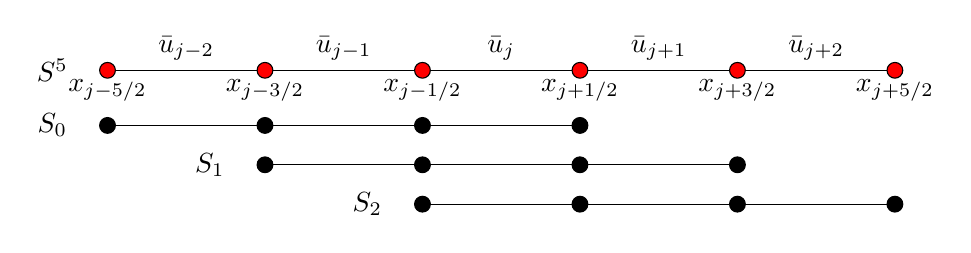
\begin{tikzpicture}
        \node[above] at (1,0) { $\bar{u}_{j-2}$ };
        \node[above] at (3,0) { $\bar{u}_{j-1}$ };
        \node[above] at (5,0) { $\bar{u}_{j}$ };
        \node[above] at (7,0) { $\bar{u}_{j+1}$ };
        \node[above] at (9,0) { $\bar{u}_{j+2}$ };

        \draw (0,0) -- (10,0);
        \foreach \x/\label in {0/{$x_{j-{5/2}}$},2/{$x_{j-{3/2}}$},4/{$x_{j-1/2}$},6/{$x_{j+1/2}$},8/{$x_{j+3/2}$},10/{$x_{j+5/2}$}} {
        \draw[fill=red] (\x,0) circle (0.1) node[below] {\label};
        }
        \node at (-0.7,0) { $S^5$ };

        \draw (0,-0.5-0.2) -- (6,-0.5-0.2);
        \foreach \x in {0,2,4,6} {
                \draw[fill=black] (\x,-0.5-0.2) circle (0.1) ;
            }
        \node at (-0.7,-0.5-0.2) { $S_0$ };

        \draw (2,-1-0.2) -- (8,-1-0.2);
        \foreach \x in {2,4,6,8} {
                \draw[fill=black] (\x,-1-0.2) circle (0.1) ;
            }
        \node at (1.3,-1-0.2) { $S_1$ };

        \draw (4,-1.5-0.2) -- (10,-1.5-0.2);
        \foreach \x in {4,6,8,10} {
                \draw[fill=black] (\x,-1.5-0.2) circle (0.1) ;
            }
        \node at (3.3,-1.5-0.2) { $S_2$ };
    \end{tikzpicture}
    \caption{大模板 $S^5(j)$ 与三个子模板 $S^3_0(j)$、$S^3_1(j)$、$S^3_2(j)$ 的示意图。}
    \label{fig:temple}
\end{figure}


设 $\hat{u}$ 为 $u(x)$ 的近似，则三个子模板对应为
\begin{equation}
\begin{aligned}
\hat{u}^{(0)}_{j+\frac{1}{2}} &= \frac{1}{6}\left(2\bar{u}_{j-2}-7\bar{u}_{j-1}+11\bar{u}_j\right),\\
\hat{u}^{(1)}_{j+\frac{1}{2}} &= \frac{1}{6}\left(-\bar{u}_{j-1}+5\bar{u}_j+2\bar{u}_{j+1}\right),\\
\hat{u}^{(2)}_{j+\frac{1}{2}} &= \frac{1}{6}\left(2\bar{u}_j+5\bar{u}_{j+1}-\bar{u}_{j+2}\right),
\end{aligned}
\end{equation}
其中上标用于区分不同子模板。

% 通过将上述表达式中所有下标整体减 $1$，可得到
% $\hat{u}^{(k)}_{i-\frac{1}{2}}$。
随后，模板 $S_5$ 上的 $\hat{u}_{j+\frac{1}{2}}$ 可表示为
\begin{equation}
\hat{u}_{j+\frac{1}{2}} = \sum_{k=0}^{2} \omega_k \hat{u}^{(k)}_{j+\frac{1}{2}}.
\end{equation}
在光滑区域中，权重趋近于其理想值：
\begin{equation}
d_0 = \frac{1}{10},\quad d_1 = \frac{6}{10},\quad d_2 = \frac{3}{10}.
\end{equation}

\subsubsection{WENO5-JS格式}

经典五阶 WENO（WENO5-JS）格式由 Jiang 和 Shu 提出，其非线性权重定义为
\begin{equation}
\alpha_k = \frac{d_k}{(\beta_k+\varepsilon)^p},\quad
\omega_k = \frac{\alpha_k}{\sum_{l=0}^2 \alpha_l},\quad k=0,1,2.
\end{equation}
其中 $\varepsilon$ 为避免分母为零的小正数，$p\ge 1$ 为幂指数（通常取 $2$），
用于控制数值耗散强度。$\beta_k$ 为第 $k$ 个子模板的光滑性指标：
\begin{equation}
\begin{aligned}
\beta_0 &= \frac{13}{12}(\bar{u}_{j-2}-2\bar{u}_{j-1}+\bar{u}_j)^2
+ \frac{1}{4}(\bar{u}_{j-2}-4\bar{u}_{j-1}+3\bar{u}_j)^2,\\
\beta_1 &= \frac{13}{12}(\bar{u}_{j-1}-2\bar{u}_j+\bar{u}_{j+1})^2
+ \frac{1}{4}(\bar{u}_{j-1}-\bar{u}_{j+1})^2,\\
\beta_2 &= \frac{13}{12}(\bar{u}_j-2\bar{u}_{j+1}+\bar{u}_{j+2})^2
+ \frac{1}{4}(3\bar{u}_j-4\bar{u}_{j+1}+\bar{u}_{j+2})^2.
\end{aligned}
\end{equation}

在光滑区域中，为达到最优阶精度，需要满足
\begin{equation}
    \hat{u}_{j+\frac{1}{2}} - u(x_{j+\frac{1}{2}}) = \mathcal{O}(\Delta x^5).
\end{equation}
对应非线性权重需满足一定条件，详见~\cite{borges2008improved}. 一个常用的强充分条件为
\begin{equation}
    \omega_k = d_k + \mathcal{O}(\Delta x^3),
\end{equation}
然而，使用taylor分析可知：
\begin{itemize}
\item 在非临界点，WENO5-JS 满足最优精度的充要条件；
\item 在临界点，仅满足 $\omega_k = d_k + \mathcal{O}(\Delta x)$，导致精度退化。
\end{itemize}

\subsubsection{WENO5-Z格式}

Borges 等提出 WENO-Z，通过引入高阶光滑性指标改进权重分配：
\begin{equation}
\beta_k^{Z} = \frac{\beta_k + \varepsilon}{\beta_k + \tau_5 + \varepsilon},
\end{equation}
其中 $\tau_5 = |\beta_0 - \beta_2|$。其性质为：
\begin{itemize}
\item 若模板光滑，则 $\tau_5 = \mathcal{O}(\Delta x^5)$；
\item 若存在间断，则 $\tau_5 = \mathcal{O}(1)$。
\end{itemize}

新的权重定义为
\begin{equation}
\alpha_k^{Z} = d_k\left(1+\frac{\tau_5}{\beta_k+\varepsilon}\right),\quad
\omega_k^{Z} = \frac{\alpha_k^{Z}}{\sum_{l=0}^2 \alpha_l^{Z}}.
\end{equation}

WENO-Z 在数值效果上优于 WENO-JS，但在临界点仍存在精度退化问题。

% $\frac{1}{\Delta x}(h_{i+\frac{1}{2}} - h_{i-\frac{1}{2}})$
% 恰好等于单元中心 $i$ 处 $f$ 的一阶导数，即 $f'_i$。

% 经典 WENO-JS 格式基于五点大模板 $S^5(j) = \{\bar{u}_{j-2}, \bar{u}_{j-1}, \bar{u}_j, \bar{u}_{j+1}, \bar{u}_{j+2}\}$，将其划分为如~\autoref{fig:temple} 所示的三个三点子模板 $S^3_k(j)$（$k = 0, 1, 2$），并对各子模板上的重构结果进行加权组合。
% 三个子模板对应的候选重构值分别为
% \begin{equation}
%     \begin{aligned}
%         \hat{u}_{j+1/2}^{0,-} & = \frac{1}{6}\bigl(2\bar{u}_{j-2} - 7\bar{u}_{j-1} + 11\bar{u}_j\bigr),  \\
%         \hat{u}_{j+1/2}^{1,-} & = \frac{1}{6}\bigl(-\bar{u}_{j-1} + 5\bar{u}_j + 2\bar{u}_{j+1}\bigr),   \\
%         \hat{u}_{j+1/2}^{2,-} & = \frac{1}{6}\bigl(2\bar{u}_j + 5\bar{u}_{j+1} - \bar{u}_{j+2}\bigr).
%     \end{aligned}
% \end{equation}
% 上述三个候选值各为三阶精度。若解在大模板上整体光滑，则对三者进行适当的线性组合可将精度提升至五阶；而在间断附近，则需根据各子模板的光滑程度自适应调整权重，以避免跨间断插值所引入的振荡。

% 为量化各子模板上解的光滑程度，Jiang 和 Shu 引入了如下光滑度指标：
% \begin{equation}
%     \beta_k = \sum_{l=1}^{2} \Delta x^{2l-1} \int_{x_{i-1/2}}^{x_{i+1/2}} \left( \frac{\mathrm{d}^l}{\mathrm{d}x^l} \hat{u}^k(x) \right)^2 \mathrm{d}x,
% \end{equation}
% 具体形式为
% \begin{equation}
%     \label{eq:beta_JS}
%     \begin{aligned}
%         \beta_0 & = \frac{13}{12}(\bar{u}_{j-2} - 2\bar{u}_{j-1} + \bar{u}_j)^2
%         + \frac{1}{4}(\bar{u}_{j-2} - 4\bar{u}_{j-1} + 3\bar{u}_j)^2,         \\
%         \beta_1 & = \frac{13}{12}(\bar{u}_{j-1} - 2\bar{u}_j + \bar{u}_{j+1})^2
%         + \frac{1}{4}(\bar{u}_{j-1} - \bar{u}_{j+1})^2,                        \\
%         \beta_2 & = \frac{13}{12}(\bar{u}_j - 2\bar{u}_{j+1} + \bar{u}_{j+2})^2
%         + \frac{1}{4}(3\bar{u}_j - 4\bar{u}_{j+1} + \bar{u}_{j+2})^2.
%     \end{aligned}
% \end{equation}
% $\beta_k$ 由子模板上数值导数的加权平方和构成，本质上度量了各子模板上数值解各阶导数的振荡幅度：当某一子模板内含间断时，对应的 $\beta_k$ 显著增大，从而在后续加权步骤中被赋予极小的权重，使该子模板对最终重构值的贡献几乎为零；在解整体光滑时，三个 $\beta_k$ 趋于相同量级，非线性权重退化为最优线性权重，格式恢复五阶精度。这一``自适应降权''机制正是 WENO 格式实现本质无振荡的核心所在。

% 最优线性权重取为 $d_0 = 1/10$，$d_1 = 3/5$，$d_2 = 3/10$，可验证此权重组合恰使线性重构达到五阶精度。基于光滑度指标，非线性权重计算如下：
% \begin{equation}
%     \tilde{\omega}_k = \frac{d_k}{(\varepsilon + \beta_k)^2},
%     \qquad
%     \omega_k = \frac{\tilde{\omega}_k}{\tilde{\omega}_0 + \tilde{\omega}_1 + \tilde{\omega}_2},
%     \quad k = 0, 1, 2,
% \end{equation}
% 其中 $\varepsilon = 10^{-6}$ 为防止分母为零而引入的小量。归一化处理保证了 $\omega_0 + \omega_1 + \omega_2 = 1$，从而使最终重构为各候选值的凸组合。最终重构值为
% \begin{equation}
%     \hat{u}_{j+1/2}^- = \omega_0 \hat{u}_{j+1/2}^{0,-} + \omega_1 \hat{u}_{j+1/2}^{1,-} + \omega_2 \hat{u}_{j+1/2}^{2,-}.
% \end{equation}

% \textcolor{red}{WENO-JS 格式存在一个已知缺陷：在解的极值点附近（即一阶导数为零处），非线性权重 $\omega_k$ 与最优线性权重 $d_k$ 之间的偏差仅为 $O(\Delta x)$，不满足维持五阶精度所需的 $\omega_k - d_k = O(\Delta x^2)$ 条件，导致格式在极值点处精度退化至三阶。针对这一问题，Borges 等人~\cite{borges2008improved} 提出了 WENOJS 格式。其核心思想是构造一个基于大模板的高阶全局光滑度指标}
% \begin{equation}
%     \tau_5 = |\beta_0 - \beta_2|,
% \end{equation}
% 并将非线性权重修改为
% \begin{equation}
%     \tilde{\omega}_k^Z = d_k\!\left(1 + \frac{\tau_5}{\beta_k + \varepsilon}\right),
%     \qquad
%     \omega_k^Z = \frac{\tilde{\omega}_k^Z}{\sum_{l=0}^{2} \tilde{\omega}_l^Z}.
% \end{equation}
% \textcolor{red}{$\tau_5$ 度量了各局部光滑度指标之间的差异：在光滑区域，$\tau_5 = O(\Delta x^5)$，而 $\beta_k = O(\Delta x^2)$，使得 $\tau_5/(\beta_k + \varepsilon) = O(\Delta x^3)$，从而 $\omega_k^Z - d_k = O(\Delta x^3)$，超出了五阶精度所需的 $O(\Delta x^2)$ 条件，即便在极值点处亦能保持五阶收敛。相较于 WENO-JS，WENOJS 格式以较低的额外计算代价显著改善了极值点附近的精度与分辨率，已成为目前工程与学术计算中应用最为广泛的高精度格式之一。}


% \subsection{WENO重构}

% 这里采用均匀网格，网格间距为 $\Delta x$，单元中心与单元边界的位置分别表示为
% $x_i = i\Delta x,\; x_{i+\frac{1}{2}} = x_i + \frac{\Delta x}{2},\; i=0,\dots,N$。
% 单元中心与单元边界处的通量值分别记为
% $f_i = f(x_i)$ 和 $f_{i+\frac{1}{2}} = f(x_{i+\frac{1}{2}})$。
% 数值通量 $h(x)$ 定义为
% \begin{equation}
% f(x)=\frac{1}{\Delta x}\int_{x-\Delta x/2}^{x+\Delta x/2} h(\xi)\, d\xi,
% \end{equation}
% 因此，
% $\frac{1}{\Delta x}(h_{i+\frac{1}{2}} - h_{i-\frac{1}{2}})$
% 恰好等于单元中心 $i$ 处 $f$ 的一阶导数，即 $f'_i$。

% %%%%%%%%%%%%%%%%%%%%%%%%%%%%%%%%%%%%%%%%%%%%%%%%%%%
% 不失一般性，以五阶 WENO（WENO5）格式为例说明重构过程。在线性格式中，
% 获得 $h(x)$ 的五阶近似仅需一个五点模板 $S_5$；
% 而在 WENO5 中，$S_5$ 被划分为三个子模板 $\{S_0,S_1,S_2\}$，
% 每个子模板包含三个相邻网格点（见图1）。
% 在光滑区域中，WENO5 采用对应的理想权重对各子模板进行加权，
% 从而获得五阶精度的近似；
% 而在存在间断的区域中，通过对包含间断的子模板赋予较小权重，
% 以避免数值振荡。

% 设 $\hat{h}$ 为 $h(x)$ 的近似，则三个子模板对应为
% \begin{equation}
% \begin{aligned}
% \hat{h}^{(0)}_{i+\frac{1}{2}} &= \frac{1}{6}\left(2f_{i-2}-7f_{i-1}+11f_i\right),\\
% \hat{h}^{(1)}_{i+\frac{1}{2}} &= \frac{1}{6}\left(-f_{i-1}+5f_i+2f_{i+1}\right),\\
% \hat{h}^{(2)}_{i+\frac{1}{2}} &= \frac{1}{6}\left(2f_i+5f_{i+1}-f_{i+2}\right),
% \end{aligned}
% \end{equation}
% 其中上标用于区分不同子模板。

% 通过将上述表达式中所有下标整体减 $1$，可得到
% $\hat{h}^{(k)}_{i-\frac{1}{2}}$。
% 随后，模板 $S_5$ 上的 $\hat{h}_{i-\frac{1}{2}}$ 可表示为
% \begin{equation}
% \hat{h}_{i-\frac{1}{2}} = \sum_{k=0}^{2} \omega_k \hat{h}^{(k)}_{i-\frac{1}{2}}.
% \end{equation}

% 在光滑区域中，权重趋近于其理想值：
% \begin{equation}
% d_0 = \frac{1}{10},\quad d_1 = \frac{6}{10},\quad d_2 = \frac{3}{10}.
% \end{equation}

% \subsection{WENO5-JS格式}

% 经典五阶 WENO（WENO5-JS）格式由 Jiang 和 Shu 提出，其非线性权重定义为
% \begin{equation}
% \alpha_k = \frac{d_k}{(\beta_k+\varepsilon)^p},\quad
% \omega_k = \frac{\alpha_k}{\sum_{l=0}^2 \alpha_l},\quad k=0,1,2.
% \end{equation}
% 其中 $\varepsilon$ 为避免分母为零的小正数，$p\ge 1$ 为幂指数（通常取 $2$），
% 用于控制数值耗散强度。$\beta_k$ 为第 $k$ 个子模板的光滑性指标：
% \begin{equation}
% \begin{aligned}
% \beta_0 &= \frac{13}{12}(f_{i-2}-2f_{i-1}+f_i)^2
% + \frac{1}{4}(f_{i-2}-4f_{i-1}+3f_i)^2,\\
% \beta_1 &= \frac{13}{12}(f_{i-1}-2f_i+f_{i+1})^2
% + \frac{1}{4}(f_{i-1}-f_{i+1})^2,\\
% \beta_2 &= \frac{13}{12}(f_i-2f_{i+1}+f_{i+2})^2
% + \frac{1}{4}(3f_i-4f_{i+1}+f_{i+2})^2.
% \end{aligned}
% \end{equation}

% 在光滑区域中，为达到最优阶精度，需要满足
% \begin{equation}
% \frac{1}{\Delta x}\left(\hat{h}_{i+\frac{1}{2}}-\hat{h}_{i-\frac{1}{2}}\right)
% = f'_i + \mathcal{O}(\Delta x^5),
% \end{equation}
% 对应权重需满足一定条件，例如强充分条件
% \begin{equation}
% \omega_k = d_k + \mathcal{O}(\Delta x^3),
% \end{equation}
% 以及较弱充分条件
% \begin{equation}
% \omega_k = d_k + \mathcal{O}(\Delta x^2).
% \end{equation}

% 对 $\beta_k$ 在 $x_i$ 处进行泰勒展开可得（略写）：
% \begin{equation}
% \beta_k = f'^2 \Delta x^2 + \mathcal{O}(\Delta x^4).
% \end{equation}

% 当 $f' \neq 0$ 时：
% \begin{equation}
% \beta_k = D\left(1+\mathcal{O}(\Delta x^2)\right),\quad D=(f'\Delta x)^2;
% \end{equation}

% 当 $f'=0, f''\neq 0$（临界点）时：
% \begin{equation}
% \beta_k = D\left(1+\mathcal{O}(\Delta x)\right).
% \end{equation}

% 由此可知：
% \begin{itemize}
% \item 在非临界点，WENO5-JS 满足最优精度的弱充分条件；
% \item 在临界点，仅满足 $\omega_k = d_k + \mathcal{O}(\Delta x)$，
% 导致精度退化。
% \end{itemize}

% \subsection{WENO5-Z格式}

% Borges 等提出 WENO-Z，通过引入高阶光滑性指标改进权重分配：
% \begin{equation}
% \beta_k^{Z} = \frac{\beta_k + \varepsilon}{\beta_k + \tau_5 + \varepsilon},
% \end{equation}
% 其中 $\tau_5 = |\beta_0 - \beta_2|$。

% 其性质为：
% \begin{itemize}
% \item 若模板光滑，则 $\tau_5 = \mathcal{O}(\Delta x^5)$；
% \item 若存在间断，则 $\tau_5 = \mathcal{O}(1)$。
% \end{itemize}

% 新的权重定义为
% \begin{equation}
% \alpha_k^{Z} = d_k\left(1+\frac{\tau_5}{\beta_k+\varepsilon}\right),\quad
% \omega_k^{Z} = \frac{\alpha_k^{Z}}{\sum_{l=0}^2 \alpha_l^{Z}}.
% \end{equation}

% WENO-Z 在数值效果上优于 WENO-JS，但在临界点仍存在精度退化问题。

% 随后，Castro 等对其进行推广，得到高阶 WENO-Z：
% \begin{equation}
% \alpha_k^{Z} = d_k\left(1+\left(\frac{\tau_{2r-1}}{\beta_k+\varepsilon}\right)^p\right),
% \quad
% \omega_k^{Z} = \frac{\alpha_k^{Z}}{\sum_{l=0}^{r-1} \alpha_l^{Z}}.
% \end{equation}

% 参数 $p$ 的作用包括：
% \begin{itemize}
% \item 控制数值耗散（$p$ 越大耗散越强）；
% \item 在临界点恢复精度（当 $p \ge 2$ 时满足最优阶条件）。
% \end{itemize}

% 通常对于 $(2r-1)$ 阶格式，建议取 $p=r-1$ 以平衡精度与稳定性。

\subsubsection{二维 WENO 重构}

% 本节将一维 WENO 重构推广至二维计算域。设单元 $I_{i,j} = [x_{i-1/2}, x_{i+1/2}] \times [y_{j-1/2}, y_{j+1/2}]$，已知单元平均值 $\bar{u}_{i,j}$，目标是在单元界面处获得高精度的左、右重构值以计算数值通量。

对于二维问题，常见的 WENO 重构方案主要分为两类：A 类方案通过对每个方向独立施加一维重构来获得界面处的线平均值；B 类方案在 A 类方案的基础上增加第二步重构，从而直接得到界面处的点值近似。下面将分别介绍这两类方案的算法流程与性能特点.



\paragraph{A 类方案（维度降维）}

A 类方案对每个方向独立地施加一维 WENO 重构，算法如下：

首先在 $y$ 方向对每列 $\{\bar{u}_{i, j+r}\}_{r}$ 实施一维 WENO 重构，
得到 $y = y_{j+1/2}$ 界面处 $u$ 的 $x$ 方向单元平均值近似：
\begin{equation}
    \bar{u}^{\pm}_{i, j+1/2}
    \approx \frac{1}{h_x}\int_{x_{i-1/2}}^{x_{i+1/2}}
    u(x, y_{j+1/2})\,\mathrm{d}x.
\end{equation}
类似地，在 $x$ 方向重构得到 $x = x_{i+1/2}$ 处的近似
$\bar{u}^{\pm}_{i+1/2, j}$。
随后直接用线平均值构造数值通量：
\begin{equation}
    \hat{f}_{i+1/2,\, j}
    = \hat{f}\!\left(\bar{u}^-_{i+1/2,j},\,\bar{u}^+_{i+1/2,j}\right),
    \qquad
    \hat{g}_{i,\, j+1/2}
    = \hat{g}\!\left(\bar{u}^-_{i,j+1/2},\,\bar{u}^+_{i,j+1/2}\right).
\end{equation}

A 类方案实现简单，计算代价低。然而，对于一般非线性系统，无论一维重构阶数多高，A 类方案的整体精度均退化为二阶，原因在于以线平均值代替积分点处点值引入了额外的截断误差。


\paragraph{B 类方案（两次重构）}

B 类方案在 A 类方案的基础上增加第二步点值重构，
从而对非线性系统也能实现高阶精度。本文采用 B 类方案，算法如下：

\begin{enumerate}
    \item 在 $y$ 方向对每列 $\{\bar{u}_{i+l, j+r}\}_{r}$ 施加一维 WENO 重构，
          得到 $y = y_{j+1/2}$ 处的 $x$ 方向单元平均值近似
          $\bar{u}^{\pm}_{i+l,\, j+1/2}$（$l = -r, \ldots, s$）。

    \item 利用步骤~1 所得的线平均值 $\bar{u}^{\pm}_{i+l,\, j+1/2}$，
          在 $x$ 方向再次施加一维 WENO 重构，
          得到界面 $y = y_{j+1/2}$ 上 Gauss--Lobatto 积分点
          $x_i^\alpha$ 处的点值近似 $u^{\pm}_{i^\alpha,\, j+1/2}$。

    \item 对 $x$ 方向界面类似处理：
          先在 $x$ 方向重构得 $\bar{u}^{\pm}_{i+1/2,\, j+r}$，
          再在 $y$ 方向重构得积分点处点值 $u^{\pm}_{i+1/2,\, j^\beta}$。

    \item 利用 Gauss--Lobatto 求积公式构造数值通量：
          \begin{equation}
            \begin{aligned}
                \hat{f}_{i+1/2,\, j}
                &= \sum_{\beta=1}^{L} \eta_\beta\,
                \hat{f}\!\left(u^-_{i+1/2,\, j^\beta},\,
                u^+_{i+1/2,\, j^\beta}\right),\\
                \hat{g}_{i,\, j+1/2}
                &= \sum_{\alpha=1}^{L} \eta_\alpha\,
                \hat{g}\!\left(u^-_{i^\alpha,\, j+1/2},\,
                u^+_{i^\alpha,\, j+1/2}\right),
            \end{aligned}
          \end{equation}
          其中 $\eta_\alpha$ 为 $L$ 点 Gauss--Lobatto 求积权重。
\end{enumerate}

B 类方案通过两次一维重构将线平均值提升为积分点处的点值，从而在数值求积意义下实现高阶精度，对非线性系统同样适用。其代价是计算量约为 A 类方案的两倍，但对于高阶方法而言，这一额外开销是实现高精度所必要的。

\begin{figure}[!htbp]
    \centering
    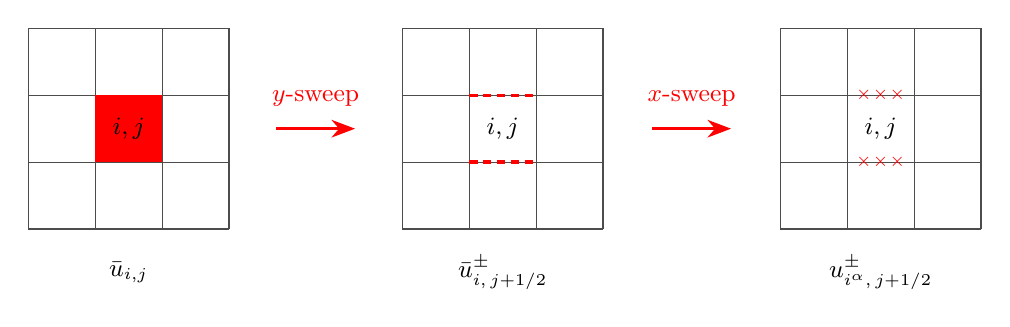
\begin{tikzpicture}[
    >=Stealth,
    font=\small,
    gridline/.style={black!70, line width=0.45pt},
    redobj/.style={red, line width=1.2pt},
    arrow/.style={red, -{Stealth[length=3mm]}, line width=0.9pt}
]

% ---------- parameters ----------
\def\dx{0.85}
\def\dy{0.85}
% Grid width = 3*\dx = 2.55cm
% Left  grid: x in [0,      2.55]
% Middle grid: x in [4.75,  7.30]   (xshift=4.75cm)
% Right  grid: x in [9.55, 12.10]   (xshift=9.55cm)
% Arrow 1 center: (2.55+4.75)/2 = 3.65cm
% Arrow 2 center: (7.30+9.55)/2 = 8.425cm

% ---------- helper: grid ----------
\newcommand{\drawgrid}[1]{
    \begin{scope}[xshift=#1]
        \foreach \x in {0,1,2,3}{
            \draw[gridline] (\x*\dx,0) -- (\x*\dx,3*\dy);
        }
        \foreach \y in {0,1,2,3}{
            \draw[gridline] (0,\y*\dy) -- (3*\dx,\y*\dy);
        }
    \end{scope}
}

% ---------- left grid ----------
\drawgrid{0cm}
\fill[red] (1*\dx,1*\dy) rectangle (2*\dx,2*\dy);
\node at (1.5*\dx,1.5*\dy) {$i,j$};
\node at (1.5*\dx,-0.55) {$\bar{u}_{i,j}$};

% ---------- arrow 1: y-sweep (centered at x=3.65cm, half-length=0.5cm) ----------
\draw[arrow] (3.15,1.5*\dy) -- (4.15,1.5*\dy);
\node[red, anchor=center] at (3.65,1.5*\dy+0.38) {$y$-sweep};

% ---------- middle grid: dashed horizontal lines at j±1/2 ----------
\begin{scope}[xshift=4.75cm]
    \drawgrid{0cm}
    \draw[redobj, densely dashed] (1*\dx,1*\dy) -- (2*\dx,1*\dy);
    \draw[redobj, densely dashed] (1*\dx,2*\dy) -- (2*\dx,2*\dy);
    \node at (1.5*\dx,1.5*\dy) {$i,j$};
    \node at (1.5*\dx,-0.55) {$\bar{u}^{\pm}_{i,\,j+1/2}$};
\end{scope}

% ---------- arrow 2: x-sweep (centered at x=8.425cm, half-length=0.5cm) ----------
\draw[arrow] (7.925,1.5*\dy) -- (8.925,1.5*\dy);
\node[red, anchor=center] at (8.425,1.5*\dy+0.38) {$x$-sweep};

% ---------- right grid: crosses along y = j±1/2 ----------
\begin{scope}[xshift=9.55cm]
    \drawgrid{0cm}
    \foreach \xx in {1.25,1.5,1.75}{
        \foreach \yy in {1,2}{
            \node[red, scale=0.75] at (\xx*\dx,\yy*\dy) {$\times$};
        }
    }
    \node at (1.5*\dx,1.5*\dy) {$i,j$};
    \node at (1.5*\dx,-0.55) {$u^{\pm}_{i^\alpha,\,j+1/2}$};
\end{scope}

\end{tikzpicture}
    \caption{}
    \label{fig:}
\end{figure}




\subsection{保正限制算法}
\label{sec:pplimiter}

% 由第~\autoref{sec:characteristic}节的特征分析可知，
% 控制方程组~\eqref{eq:governing}保持双曲性的必要条件为
% $\tilde{\rho}_k > 0$（$k = 1, 2$）。
% 为此，

定义物理可容许状态集为
\begin{equation}
    \label{eq:SET}
    \mathbb{G} = \left\{
    \bm{Q} = [\tilde{\rho}_1,\, \tilde{\rho}_2,\, \rho\bm{u}]^\top
    \;\middle|\;
    \tilde{\rho}_k > 0,\; k = 1, 2
    \right\}.
\end{equation}
为确保数值解在整个模拟过程中始终保持在可容许集 $\mathbb{G}$ 内，
本文设计了一套保正限制算法，该算法由以下两个步骤构成：
\begin{enumerate}
    \item 通过凸分解保证单元平均数值解的正性；
    \item 通过施加保正限制器保证高阶重构解的正性。
\end{enumerate}

\paragraph{单元平均值的正性保持}

考虑单元 $I_{i,j} \in \Omega$，
采用前向 Euler 时间离散的有限体积格式~\eqref{eq:fv_euler}
可以改写为如下凸分解形式。
首先，利用 Gauss--Lobatto 求积公式，
单元平均守恒变量可表示为
\begin{equation}
    \label{eq:QAVE}
    \begin{aligned}
        \overline{\bm{Q}}_{i,j}^n
        = \;&(1 - 2\omega_1)\,\bm{Q}_{i,j}^n(x_i^*, y_j^*)  \\
        &+ \mu_x\omega_1 \sum_{\beta=1}^{L} \omega_\beta
        \left(
        \bm{Q}_{i-1/2,\beta}^{n,+} + \bm{Q}_{i+1/2,\beta}^{n,-}
        \right) \\
        &+ \mu_y\omega_1 \sum_{\alpha=1}^{L} \omega_\alpha
        \left(
        \bm{Q}_{\alpha,j-1/2}^{n,+} + \bm{Q}_{\alpha,j+1/2}^{n,-}
        \right),
    \end{aligned}
\end{equation}
其中 $\omega_1$ 为 Gauss--Lobatto 求积公式端点处的求积权重，
\begin{equation}
    \mu_x = \frac{\lambda_x S_x}{\lambda_x S_x + \lambda_y S_y},
    \qquad \mu_y = 1 - \mu_x,
    \qquad \lambda_x = \frac{\Delta t}{\Delta x},
    \qquad \lambda_y = \frac{\Delta t}{\Delta y},
\end{equation}
辅助点处的值 $\bm{Q}_{i,j}^n(x_i^*, y_j^*)$ 由式~\eqref{eq:QAVE}
隐式定义。

在此基础上，引入以下引理。

\begin{lemma}
    \label{lemma:pp}
    设 $\bm{Q}_1, \bm{Q}_2, \bm{Q}_3 \in \mathbb{G}$。
    在 CFL 条件 $\lambda_x S_x \leqslant 1$，
    $\lambda_y S_y \leqslant 1$ 下，有
    \begin{equation}
        \begin{aligned}
            \bm{H}_x(\lambda_x;\, \bm{Q}_1, \bm{Q}_2, \bm{Q}_3)
            &\coloneqq \bm{Q}_2
            - \lambda_x\bigl[
            \hat{\bm{F}}_x(\bm{Q}_2, \bm{Q}_3)
            - \hat{\bm{F}}_x(\bm{Q}_1, \bm{Q}_2)
            \bigr] \in \mathbb{G}, \\
            \bm{H}_y(\lambda_y;\, \bm{Q}_1, \bm{Q}_2, \bm{Q}_3)
            &\coloneqq \bm{Q}_2
            - \lambda_y\bigl[
            \hat{\bm{F}}_y(\bm{Q}_2, \bm{Q}_3)
            - \hat{\bm{F}}_y(\bm{Q}_1, \bm{Q}_2)
            \bigr] \in \mathbb{G}.
        \end{aligned}
    \end{equation}
\end{lemma}
\begin{proof}
    该引理可通过直接计算验证，此处略去。
\end{proof}

基于引理~\autoref{lemma:pp}，可以建立单元平均值正性保持的充分条件。

\begin{theorem}
    \label{thm:cell_avg_pp}
    若由 WENO 重构得到的界面值满足
    $\bm{Q}_{i\pm 1/2, \beta}^{n,\pm} \in \mathbb{G}$，
    $\bm{Q}_{\alpha, j\pm 1/2}^{n,\pm} \in \mathbb{G}$，
    且辅助点值满足 $\bm{Q}_{i,j}^n(x_i^*, y_j^*) \in \mathbb{G}$，
    则在 CFL 条件
    \begin{equation}
        \label{eq:cfl_pp}
        \Delta t \leqslant
        \frac{\omega_1}{S_x/\Delta x + S_y/\Delta y}
    \end{equation}
    下，有 $\overline{\bm{Q}}_{i,j}^{n+1} \in \mathbb{G}$。
\end{theorem}

\begin{proof}
    将格式~\eqref{eq:fv_euler}通过添加辅助项改写为：
    \begin{equation}
        \label{eq:AVE_decomp}
        \begin{aligned}
            \overline{\bm{Q}}_{i,j}^{n+1}
            = \overline{\bm{Q}}_{i,j}^n
            &- \lambda_x \sum_{\alpha=1}^{L} \omega_\alpha
            \Bigl[
            \hat{\bm{F}}_x(\bm{Q}_{\alpha,j+1/2}^{n,-},\,
            \bm{Q}_{\alpha,j+1/2}^{n,+})
            - \hat{\bm{F}}_x(\bm{Q}_{\alpha,j-1/2}^{n,+},\,
            \bm{Q}_{\alpha,j+1/2}^{n,-})
            \Bigr] \\
            &- \lambda_x \sum_{\alpha=1}^{L} \omega_\alpha
            \Bigl[
            \hat{\bm{F}}_x(\bm{Q}_{\alpha,j-1/2}^{n,+},\,
            \bm{Q}_{\alpha,j+1/2}^{n,-})
            - \hat{\bm{F}}_x(\bm{Q}_{\alpha,j-1/2}^{n,-},\,
            \bm{Q}_{\alpha,j-1/2}^{n,+})
            \Bigr] \\
            &- \lambda_y \sum_{\beta=1}^{L} \omega_\beta
            \Bigl[
            \hat{\bm{F}}_y(\bm{Q}_{i+1/2,\beta}^{n,-},\,
            \bm{Q}_{i+1/2,\beta}^{n,+})
            - \hat{\bm{F}}_y(\bm{Q}_{i-1/2,\beta}^{n,+},\,
            \bm{Q}_{i+1/2,\beta}^{n,-})
            \Bigr] \\
            &- \lambda_y \sum_{\beta=1}^{L} \omega_\beta
            \Bigl[
            \hat{\bm{F}}_y(\bm{Q}_{i-1/2,\beta}^{n,+},\,
            \bm{Q}_{i+1/2,\beta}^{n,-})
            - \hat{\bm{F}}_y(\bm{Q}_{i-1/2,\beta}^{n,-},\,
            \bm{Q}_{i-1/2,\beta}^{n,+})
            \Bigr].
        \end{aligned}
    \end{equation}
    将凸分解式~\eqref{eq:QAVE}代入式~\eqref{eq:AVE_decomp}，整理得
    \begin{equation}
        \label{eq:convex_decomp}
        \begin{aligned}
            \overline{\bm{Q}}_{i,j}^{n+1}
            = \;&(1-2\omega_1)\,\bm{Q}_{i,j}^n(x_i^*, y_j^*) \\
            &+ \mu_x \omega_1 \sum_{\alpha=1}^{L} \omega_\alpha\,
            \bm{H}_x\!\left(
            \frac{\lambda_x}{\mu_x\omega_1};\,
            \bm{Q}_{\alpha,j-1/2}^{n,+},\,
            \bm{Q}_{\alpha,j+1/2}^{n,-},\,
            \bm{Q}_{\alpha,j+1/2}^{n,+}
            \right) \\
            &+ \mu_x \omega_1 \sum_{\alpha=1}^{L} \omega_\alpha\,
            \bm{H}_x\!\left(
            \frac{\lambda_x}{\mu_x\omega_1};\,
            \bm{Q}_{\alpha,j-1/2}^{n,-},\,
            \bm{Q}_{\alpha,j-1/2}^{n,+},\,
            \bm{Q}_{\alpha,j+1/2}^{n,-}
            \right) \\
            &+ \mu_y \omega_1 \sum_{\beta=1}^{L} \omega_\beta\,
            \bm{H}_y\!\left(
            \frac{\lambda_y}{\mu_y\omega_1};\,
            \bm{Q}_{i-1/2,\beta}^{n,+},\,
            \bm{Q}_{i+1/2,\beta}^{n,-},\,
            \bm{Q}_{i+1/2,\beta}^{n,+}
            \right) \\
            &+ \mu_y \omega_1 \sum_{\beta=1}^{L} \omega_\beta\,
            \bm{H}_y\!\left(
            \frac{\lambda_y}{\mu_y\omega_1};\,
            \bm{Q}_{i-1/2,\beta}^{n,-},\,
            \bm{Q}_{i-1/2,\beta}^{n,+},\,
            \bm{Q}_{i+1/2,\beta}^{n,-}
            \right).
        \end{aligned}
    \end{equation}
    式~\eqref{eq:convex_decomp}是 $\bm{Q}_{i,j}^n(x_i^*, y_j^*)$
    及各 $\bm{H}_x$、$\bm{H}_y$ 项的凸组合
    （各系数非负且和为 $1$，可由 $\sum_\alpha \omega_\alpha = 1$
    及 $\mu_x + \mu_y = 1$ 验证）。
    在 CFL 条件~\eqref{eq:cfl_pp}下，
    $\lambda_x/(\mu_x\omega_1) \cdot S_x \leqslant 1$
    且 $\lambda_y/(\mu_y\omega_1) \cdot S_y \leqslant 1$，
    由引理~\autoref{lemma:pp}知各 $\bm{H}_x$、$\bm{H}_y$ 项均属于 $\mathbb{G}$。
    由假设条件知 $\bm{Q}_{i,j}^n(x_i^*, y_j^*) \in \mathbb{G}$，
    故凸组合~\eqref{eq:convex_decomp}属于凸集 $\mathbb{G}$，
    即 $\overline{\bm{Q}}_{i,j}^{n+1} \in \mathbb{G}$。
\end{proof}

\paragraph{高阶重构解的保正限制器}

为满足定理~\autoref{thm:cell_avg_pp}的前提条件，
对 WENO 重构所得多项式解施加如下缩放型保正限制器~\cite{zhang2011maximum}：
\begin{equation}
    \label{eq:pp_limiter}
    \widetilde{\bm{Q}}_{i,j}^n(x, y)
    = \theta\left(\bm{Q}_{i,j}^n(x,y) - \overline{\bm{Q}}_{i,j}^n\right)
    + \overline{\bm{Q}}_{i,j}^n,
\end{equation}
其中缩放因子 $\theta \in [0, 1]$ 定义为
\begin{equation}
    \label{eq:theta}
    \theta = \min_{k=1,2}\, \theta_k,
    \qquad
    \theta_k = \min\left\{
    \frac{\overline{(\tilde{\rho}_k)}_{i,j}^n - \varepsilon_k}
    {\overline{(\tilde{\rho}_k)}_{i,j}^n - m_k},\;
    1
    \right\},
\end{equation}
其中 
\begin{equation}
    \varepsilon_k = \min\!\left\{10^{-13},\,
\overline{(\tilde{\rho}_k)}_{i,j}^n\right\}, \qquad m_k = \min_{(x,y)\,\in\,\mathcal{S}_{i,j}\,\cup\,\{(x_i^*,\,y_j^*)\}}
    (\tilde{\rho}_k)_{i,j}^n(x, y),
\end{equation}
$\mathcal{S}_{i,j}$ 为单元 $I_{i,j}$ 边界上所有 Gauss--Lobatto
积分点的集合。当 $\theta = 1$ 时限制器不起作用；
当 $\theta \to 0$ 时重构解退化为单元平均值。

保正限制器~\eqref{eq:pp_limiter}在修正重构解的同时，能够保持孤立相界面处的压力与速度均匀性。
\begin{theorem}[保正限制器的速度压力平衡性]
    \label{thm:pp_upv}
    若 $p_{i,j}^n \equiv p_0$ 且 $\bm{u}_{i,j}^n \equiv \bm{u}_0$，
    则经保正限制器~\eqref{eq:pp_limiter}修正后的重构解满足
    $\widetilde{p}_{i,j}^n \equiv p_0$ 且
    $\widetilde{\bm{u}}_{i,j}^n \equiv \bm{u}_0$，
    $\forall\, I_{i,j} \in \Omega$。
\end{theorem}

\begin{proof}
    在均匀压力与速度条件下，
    $\rho_k \equiv \rho_{k,0}$，即
    $\tilde{\rho}_k = z_k\rho_{k,0}$。
    由限制器~\eqref{eq:pp_limiter}，修正后的分相密度为
    \begin{equation}
        \widetilde{\tilde{\rho}}_k(x,y)
        = \theta\bigl(\tilde{\rho}_k(x,y) - \overline{\tilde{\rho}}_k\bigr)
        + \overline{\tilde{\rho}}_k
        = \rho_{k,0}\bigl[\theta(z_k(x,y) - \overline{z}_k) + \overline{z}_k\bigr]
        \eqqcolon \rho_{k,0}\,\widetilde{z}_k(x,y).
    \end{equation}
    因此修正后的相密度为
    $\widetilde{\rho}_k = \widetilde{\tilde{\rho}}_k / \widetilde{z}_k = \rho_{k,0}$，
    由等熵状态方程~\eqref{eq:eos_single}得
    $\widetilde{p} \equiv p_0$，压力均匀性得证。

    对于速度，修正后的混合动量为
    \begin{equation}
        \widetilde{\rho u}(x,y)
        = \theta\bigl(\rho u(x,y) - \overline{\rho u}\bigr) + \overline{\rho u}
        = \theta\bigl(\rho(x,y) - \overline{\rho}\bigr)u_0 + \overline{\rho}\,u_0
        = \widetilde{\rho}(x,y)\,u_0,
    \end{equation}
    其中利用了 $\rho u = \rho\, u_0$ 及
    $\widetilde{\rho} = \widetilde{\tilde{\rho}}_1 + \widetilde{\tilde{\rho}}_2$。
    因此 $\widetilde{u} = \widetilde{\rho u}/\widetilde{\rho} = u_0$，
    速度均匀性得证。$v$ 方向同理。
\end{proof}

\subsection{Riemann 求解器}
\label{sec:riemann}

有限体积法的核心在于对单元界面处的法向数值通量进行估计。在双曲守恒律框架下，相邻单元在界面两侧给出的重构值 $\bm{Q}_L$ 与 $\bm{Q}_R$ 构成一个局部 Riemann 问题：
\begin{equation}
    \frac{\partial \bm{Q}}{\partial t}
    + \nabla \cdot \bm{F}(\bm{Q}) = \bm{0},
    \qquad
    \bm{Q}(x, 0) =
    \begin{cases}
        \bm{Q}_L, & x < 0, \\
        \bm{Q}_R, & x > 0.
    \end{cases}
\end{equation}
Riemann 求解器的作用即是基于该初值问题的波系结构，构造界面处的数值通量 $\hat{\bm{F}}(\bm{Q}_L, \bm{Q}_R)$，以替代精确解所需的复杂迭代过程~\cite{toro2009riemann}。%对于多维问题，通常采用维度分裂或法向投影的方式，将多维 Riemann 问题化归为沿界面法方向的一维问题进行处理。

近似 Riemann 求解器按照其对波系结构的建模方式可分为多类。最简单的一类仅利用界面处的最大特征波速进行耗散控制，以局部 Lax--Friedrichs（LLF）通量为代表；更精细的一类则显式考虑多波结构，如HLLC(Harten–Lax–van Leer Contact)求解器。本节分别介绍上述两类求解器在本文格式中的具体形式。

%------------------------------------------------------------
\paragraph{LLF Riemann 求解器}

局部 Lax--Friedrichs（LLF）通量基于单波假设，不显式区分接触波、激波等各类特征波，结构最为简洁，但数值耗散相对较大。$x$ 方向和 $y$ 方向的 LLF 通量分别定义为：
\begin{equation}
    \label{eq:llf}
    \begin{aligned}
        \hat{\bm{F}}_x(\bm{Q}_L, \bm{Q}_R)
         & = \frac{1}{2}\left[\bm{F}_x(\bm{Q}_L) + \bm{F}_x(\bm{Q}_R)\right]
        - \frac{S_x}{2}\left(\bm{Q}_R - \bm{Q}_L\right), \\
        \hat{\bm{F}}_y(\bm{Q}_L, \bm{Q}_R)
         & = \frac{1}{2}\left[\bm{F}_y(\bm{Q}_L) + \bm{F}_y(\bm{Q}_R)\right]
        - \frac{S_y}{2}\left(\bm{Q}_R - \bm{Q}_L\right),
    \end{aligned}
\end{equation}
其中 $S_x = \max_{i,j}(|u_{i,j}| + c_{i,j})$ 与$S_y = \max_{i,j}(|v_{i,j}| + c_{i,j})$ 分别为$x$ 方向和 $y$ 方向上雅可比矩阵的局部最大绝对特征值。

%------------------------------------------------------------
\paragraph{HLLC Riemann 求解器}
HLL 求解器~\cite{harten1983upstream} 在 LLF 的基础上引入两波假设，以左行最快波速 $S_L$ 和右行最快波速 $S_R$ 划定星区，从而将波系结构细化为三个区域。然而，两波假设在星区内仅保留平均状态，无法分辨接触间断，在密度场的捕捉上存在明显的数值耗散。为此，Toro 等人~\cite{toro1994restoration} 在 HLL 框架内引入第三个波——接触波（中间波），构成 HLLC求解器，如~\autoref{fig:hllc} 所示。HLLC 求解器的三波假设将求解域划分为四个区域：左状态区、左星区、右星区和右状态区，各星区内的守恒变量通过对应侧的 Rankine--Hugoniot 条件和星区一致性条件（法向速度与压力在接触波两侧连续）唯一确定。
\begin{figure}[htbp]
    \centering
    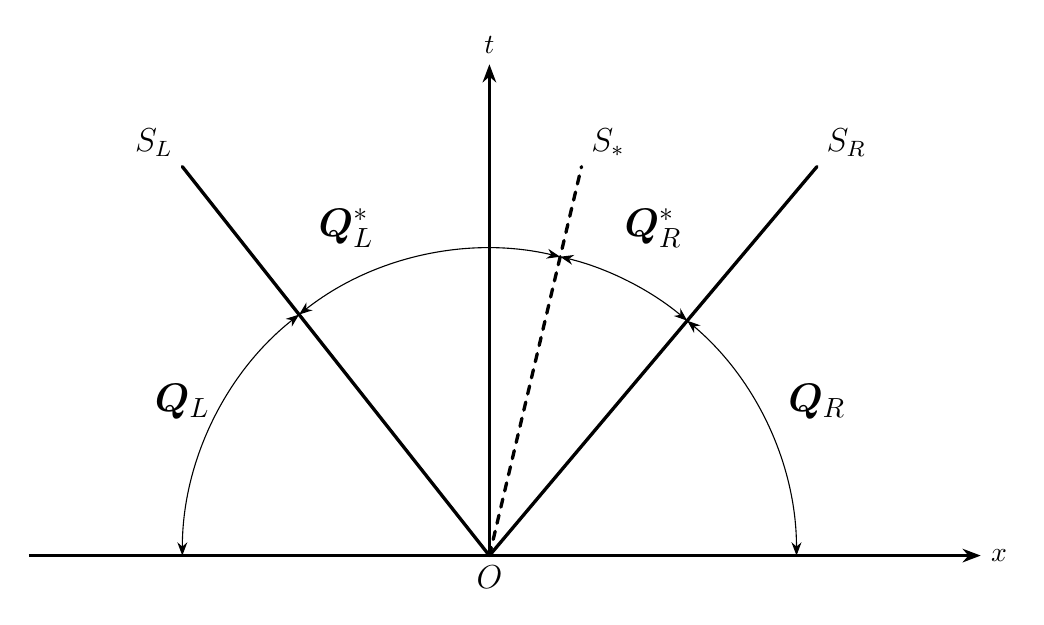
\begin{tikzpicture}[
    >=Stealth,
    scale=1.3,
    wave/.style={very thick, line cap=round},
    contact/.style={very thick, dashed, line cap=round},
    axis/.style={->, thick}
]
 
% === 坐标轴 ===
\draw[axis] (-4.5, 0) -- (4.8, 0) node[right] {$x$};
\draw[axis] (0, 0.0) -- (0, 4.8) node[above] {$t$};
\node[below, font=\large] at (0, 0) {$O$};
 
% === 左激波 S_L ===
\draw[wave] (0,0) -- (-3.0, 3.8);
\node[font=\large, above left] at (-3.0, 3.8) {$S_L$};
 
% === 右激波 S_R ===
\draw[wave] (0,0) -- (3.2, 3.8);
\node[font=\large, above right] at (3.2, 3.8) {$S_R$};
 
% === 接触间断 S_M（虚线）===
\draw[contact] (0,0) -- (0.9, 3.8);
\node[font=\large, above right] at (0.9, 3.8) {$S_*$};
 
% === 区域标注 ===
\node[font=\Large] at (-3.0, 1.5) {$\bm{Q}_L$};
\node[font=\Large] at (-1.4, 3.2) {$\bm{Q}_L^*$};  % 左上角移动
\node[font=\Large] at (1.6,  3.2) {$\bm{Q}_R^*$};
\node[font=\Large] at ( 3.2, 1.5) {$\bm{Q}_R$};
 
% ===================================================================
% 四段弧，圆心(0,0)，半径3，顺时针，双向箭头
% ===================================================================
 
% 弧1: x_neg(-3,0) [180°] --> S_L交点(-1.8589, 2.3546) [128.29°]
\draw[{Stealth}-{Stealth}, thin] (-3.000000, 0.000000)
    arc[start angle=180.0000, end angle=128.2902, radius=3];
 
% 弧2: S_L交点(-1.8589, 2.3546) [128.29°] --> S_M交点(0.6914, 2.9192) [76.68°]
\draw[{Stealth}-{Stealth}, thin] (-1.858933, 2.354648)
    arc[start angle=128.2902, end angle=76.6755, radius=3];
 
% 弧3: S_M交点(0.6914, 2.9192) [76.68°] --> S_R交点(1.9324, 2.2947) [49.90°]
\draw[{Stealth}-{Stealth}, thin] (0.691399, 2.919241)
    arc[start angle=76.6755, end angle=49.8991, radius=3];
 
% 弧4: S_R交点(1.9324, 2.2947) [49.90°] --> x_pos(3,0) [0°]
\draw[{Stealth}-{Stealth}, thin] (1.932407, 2.294734)
    arc[start angle=49.8991, end angle=0.0000, radius=3];
 
\end{tikzpicture}
    \caption{HLLC Riemann 求解器的波系结构示意图。}
    \label{fig:hllc}
\end{figure}
    
弱可压缩两相流框架下 HLLC 求解器的完整推导详见文献~\cite{zhang2025positivity}，本节直接给出相关结果。设 $S_L$ 与 $S_R$ 分别为界面处向左和向右传播的最快波速，由如下估计给出：
\begin{equation}
    \begin{aligned}
        S_L &= \min\!\left(\bm{n} \cdot \bm{u}_L - c_L,\;
    \bm{n} \cdot \bm{u}^{\mathrm{Roe}} - c^{\mathrm{Roe}}\right),\\ 
    S_R &= \max\!\left(\bm{n} \cdot \bm{u}_R + c_R,\;
    \bm{n} \cdot \bm{u}^{\mathrm{Roe}} + c^{\mathrm{Roe}}\right),
    \end{aligned}
\end{equation}
其中 $\bm{u}^{\mathrm{Roe}}$ 与 $c^{\mathrm{Roe}}$ 为 Roe 平均量~\cite{einfeldt1988godunov}，
定义为
\begin{equation}
    \begin{aligned}
        \bm{n} \cdot \bm{u}^{\mathrm{Roe}}
    &= \frac{\bm{n} \cdot \bm{u}_L \sqrt{\rho_L}
    + \bm{n} \cdot \bm{u}_R \sqrt{\rho_R}}
    {\sqrt{\rho_L} + \sqrt{\rho_R}},\\
    \left(c^{\mathrm{Roe}}\right)^2
    &= \frac{c_L^2 \sqrt{\rho_L} + c_R^2 \sqrt{\rho_R}}
    {\sqrt{\rho_L} + \sqrt{\rho_R}}
    + \frac{\sqrt{\rho_L}\sqrt{\rho_R}}
    {2\left(\sqrt{\rho_L} + \sqrt{\rho_R}\right)^2}
    \left(\bm{n} \cdot \bm{u}_R - \bm{n} \cdot \bm{u}_L\right)^2.
    \end{aligned}
\end{equation}
HLLC 型数值通量定义为
\begin{equation}
    \label{eq:hllc_flux}
    \bm{n} \cdot \hat{\bm{F}}^{\mathrm{HLLC}}(\bm{Q}_L, \bm{Q}_R) =
    \begin{cases}
        \bm{n} \cdot \bm{F}_L,      & S_L > 0,                              \\
        \bm{n} \cdot \bm{F}_{L,*},  & S_L \leqslant 0 < S_*,               \\
        \bm{n} \cdot \bm{F}_{R,*},  & S_* \leqslant 0 \leqslant S_R,       \\
        \bm{n} \cdot \bm{F}_R,      & S_R < 0,
    \end{cases}
\end{equation}
其中 $S_*$ 为接触波速（星区中间波速）。在非线性波两侧应用 Rankine--Hugoniot 跳跃条件，可得
\begin{equation}
    \label{eq:rh}
    \bm{n} \cdot (\bm{F}_{Q,*} - \bm{F}_Q) = S_Q(\bm{Q}_{Q,*} - \bm{Q}_Q),
    \quad Q = L,\, R.
\end{equation}
对速度场和压力场施加星区一致性条件
$\bm{n} \cdot \bm{u}_{L,*} = \bm{n} \cdot \bm{u}_{R,*} = S_*$，
$p_{L,*} = p_{R,*} = p_*$，
联立式~\eqref{eq:rh} 各分量，解得
\begin{equation}
    \begin{aligned}
        S_* &= \frac{p_R - p_L
    + \rho_L\,(\bm{n} \cdot \bm{u}_L)\,(S_L - \bm{n} \cdot \bm{u}_L)
    - \rho_R\,(\bm{n} \cdot \bm{u}_R)\,(S_R - \bm{n} \cdot \bm{u}_R)}
    {\rho_L(S_L - \bm{n} \cdot \bm{u}_L) - \rho_R(S_R - \bm{n} \cdot \bm{u}_R)}, \\ 
    p_* &= p_L + \rho_L(S_L - \bm{n} \cdot \bm{u}_L)(S_* - \bm{n} \cdot \bm{u}_L).
    \end{aligned}
\end{equation}
星区守恒变量为
\begin{equation}
    \label{eq:hllc_wstar}
    \bm{Q}_{Q,*} =
    \chi_{Q,*}
    \begin{pmatrix}
        (\tilde{\rho}_1)_Q                                          \\
        (\tilde{\rho}_2)_Q                                          \\
        \rho_Q\bigl[u_Q + (S_* - \bm{n} \cdot \bm{u}_Q)\, n_x\bigr] \\
        \rho_Q\bigl[v_Q + (S_* - \bm{n} \cdot \bm{u}_Q)\, n_y\bigr]
    \end{pmatrix},
    \qquad
    \chi_{Q,*} = \frac{S_Q - \bm{n} \cdot \bm{u}_Q}{S_Q - S_*}.
\end{equation}
将式~\eqref{eq:hllc_wstar} 代入式~\eqref{eq:rh}，即可得到弱可压缩两相流的完整 HLLC 数值通量~\eqref{eq:hllc_flux}。

\cleardoublepage
\section{高精度 WENO 重构}

\subsection{非多项式函数重构方法}
\label{sec:recon}
考虑一维均匀网格划分，记计算单元为 $I_j = [x_{j-1/2}, x_{j+1/2}]$，网格尺寸为 $h$。设函数 $v(x)$ 在模板
\begin{equation}
    S^n(j) = \{I_{j-r}, I_{j-r+1}, \ldots, I_{j+s}\}
\end{equation}
上的单元平均值为
\begin{equation}
    \bar{v}_i = \frac{1}{h}\int_{I_i} v(\xi)\,\mathrm{d}\xi, \quad I_i \in S^n(j),
\end{equation}
其中 $n = r + s + 1$。

本小节的目标是在给定单元平均值的基础上，在函数空间 $\Omega_n$ 中构造重构函数 $\hat{v}(x)$，以实现对原函数 $v(x)$ 的 $n$ 阶精度逼近。

传统 WENO 格式通常选取 $\Omega_n$ 为 $n-1$ 次多项式空间。然而，多项式基函数在处理具有大梯度或间断的流动问题时，其局部调节能力有限，容易引入较大的数值耗散。为此，本文考虑引入带形状参数 $\lambda$ 的非多项式逼近空间
\begin{equation}
    \Omega_n(x, j, \lambda)
    = \mathrm{span}\bigl\{
    \varphi_0(x - x_j;\, \lambda),\;
    \varphi_1(x - x_j;\, \lambda),\;
    \ldots,\;
    \varphi_{n-1}(x - x_j;\, \lambda)
    \bigr\} \subset C^\infty(\mathbb{R}),
\end{equation}
其中参数 $\lambda$ 可用于调节基函数的局部形状。

\paragraph{方法一：基于守恒约束的积分重构}

该方法通过使用单元平均守恒约束来确定重构函数。对于任意单元 $I_i \in S(j)$，要求重构函数 $\hat{v}(x)$ 满足
\begin{equation}
    \int_{I_i} \hat{v}(x)\,\mathrm{d}x = \bar{v}_i\,h.
\end{equation}
设 $\hat{v}(x)$ 属于有限维函数空间 $\Omega_n(x, j, \lambda)$，则可表示为
\begin{equation}
    \hat{v}(x) = \sum_{k=0}^{n-1} c_k\,\varphi_k(x - x_j;\, \lambda).
\end{equation}
将其代入守恒约束条件，可得到关于系数向量 $\bm{c}$ 的线性方程组
\begin{equation}
    \bm{A}\,\bm{c} = \bm{b},
\end{equation}
其中
\begin{equation}
    \bm{A}_{ik} = \int_{I_i} \varphi_k(x)\,\mathrm{d}x, \qquad
    \bm{b}_i = \bar{v}_i\,h.
\end{equation}
当矩阵 $\bm{A}$ 非奇异时，该线性系统存在唯一解，从而唯一确定重构函数 $\hat{v}(x)$。

\paragraph{方法二：基于原函数的重构方法}

该方法源于经典 WENO 重构思想，即通过构造原函数的插值函数并求导来获得重构结果。

设 $v(x)$ 的一个原函数为
\begin{equation}
    H(x) = \int_{-\infty}^{x} v(t)\,\mathrm{d}t,
\end{equation}
则有
\begin{equation}
    H(x_{i+1/2}) - H(x_{i-1/2}) = \int_{I_i} v(x)\,\mathrm{d}x = \bar{v}_i\,h.
\end{equation}
因此，通过累加单元平均值，可以在界面点构造 $H(x)$ 的离散表示（常数项对后续求导无影响，故可忽略）。



在插值节点集
\begin{equation}
    S_m = \bigl\{x_{j-r-1/2},\, x_{j-r+1/2},\, \ldots,\, x_{j+s+1/2}\bigr\}
\end{equation}
上，构造 $H(x)$ 的插值函数
\begin{equation}
    H_{n+1}(x) = \sum_{m=0}^{n} H\!\left(x_{j-r+m-1/2}\right) L_m(x),
\end{equation}
其中 $L_m(x)$ 为满足
\begin{equation}
    L_m\!\left(x_{j-r+k-1/2}\right) = \delta_{mk}, \quad k = 0,1, \ldots, n
\end{equation}
的插值基函数。

定义重构函数为
\begin{equation}
    \hat{v}(x) := \frac{\mathrm{d}}{\mathrm{d}x} H_{n+1}(x),
\end{equation}
则界面 $x_{j+1/2}$ 处的重构值为
\begin{equation}
    \hat{v}_{j+1/2} = H_{n+1}'\!\left(x_{j+1/2}\right)
    = \sum_{m=0}^{n} H\!\left(x_{j-r+m-1/2}\right) L_m'\!\left(x_{j+1/2}\right).
\end{equation}

为保证 $\hat{v}(x) \in \Omega_n$，构造辅助函数
\begin{equation}
    \phi_0(x) = 1, \quad \phi_k(x) = \int_{-\infty}^x \varphi_{k-1}(t - x_j)\,\mathrm{d}t, \quad k = 1,2,\ldots,n,
\end{equation}
并要求插值基函数满足
\begin{equation}
    \sum_{k=0}^{n} \phi_\ell\!\left(x_{j-r+k-1/2}\right)\,L_k(x)= \phi_\ell(x),
    \quad \ell = 0,1,\ldots,n.
\end{equation}


当矩阵 $\bm{A} = \{\phi_\ell(x_{j-r+k-1/2})\}$ 非奇异时，插值基函数唯一确定，从而完成重构。

\begin{remark}
    方法一与方法二在重构结果上是等价的。事实上，由方法二构造的重构函数
    \begin{equation}
        \hat{v}(x) = H_{n+1}'(x)
    \end{equation}
    同样满足单元平均守恒约束。对任意单元 $I_j = [x_{j-1/2}, x_{j+1/2}]$，有
    \begin{equation}
    \int_{I_j} \hat{v}(x)\,\mathrm{d}x
    = H_{n+1}(x_{j+1/2}) - H_{n+1}(x_{j-1/2}) = \bar{v}_j\,h.
    \end{equation}
    因此，方法二得到的重构函数同样满足方法一中的积分守恒条件。在矩阵可逆的条件下，两种方法得到的重构函数唯一，从而二者是等价的。
\end{remark}

\subsection{非多项式基函数}

为使非多项式重构具备高精度与良好的数值性质，对函数空间 $\Omega_n$ 提出以下约束条件。

\begin{property}[积分矩阵可逆性]
    \label{prop:nonpol_integral_matrix}
    定义积分矩阵
    \begin{equation}
        \bm{A}_{i,k} = \int_{I_i} \varphi_k(x)\,\mathrm{d}x,
    \end{equation}
    要求矩阵 $\bm{A}$ 非奇异。
\end{property}

\begin{property}[包含常数]
    \label{prop:nonpol_const}
    函数空间 $\Omega_n$ 必须包含常数函数，即 $1 \in \Omega_n$。
\end{property}

\begin{property}[对称性]
    \label{prop:nonpol_symmetry}
    若 $\varphi_k(x+x_j;\lambda) \in \Omega_n$，则 $\varphi_k(-x+x_j;\lambda) \in \Omega_n$。
\end{property}

\begin{property}[渐近多项式再现性]
    \label{prop:nonpol_asymp_poly}
    存在系数向量 $\bm{c}_\ell(\lambda)$，使得对于 $\ell = 0, 1, \ldots, n-1$，一致成立
    \begin{equation}
        x^\ell - \sum_{i=0}^{n-1} c_{\ell,i}(\lambda)\,\varphi_i(x;\lambda)
        = c(\lambda)\,\mathcal{O}(\Delta x^n), \quad \lambda \to 0,
    \end{equation}
    其中 $c(\lambda)$ 为关于 $\lambda$ 的某一函数，满足 $\lim_{\lambda \to 0} c(\lambda) = 0$。
\end{property}

基于满足上述条件的函数空间所构造的重构函数具有如下性质。

\begin{theorem}[常数函数的精确重构]
    \label{thm:nonpol_const}
    若原函数 $v(x)$ 为常数函数，则由非多项式空间 $\Omega_n$ 构造的重构函数 $\hat{v}(x)$
    亦为相同的常数函数。该性质有助于保持质量守恒性，以及孤立相界面处压力与速度的均匀性。
\end{theorem}

\begin{proof}
    设 $v(x) \equiv c$，由性质~\ref{prop:nonpol_const}，常数函数 $c \in \Omega_n$，可验证其满足全部单元平均守恒约束；再由性质~\ref{prop:nonpol_integral_matrix}，矩阵 $\bm{A}$ 非奇异，解唯一，故 $\hat{v}(x) \equiv c$。
\end{proof}

\begin{theorem}[非多项式重构的对称性]
    \label{thm:nonpol_symmetry}
    对两个关于某一界面对称的模板
    \begin{equation}
        S^L = \{I_{j-r}, I_{j-r+1}, \ldots, I_{j+s}\},\qquad
        S^R = \{I_{\tilde{j}-s}, I_{\tilde{j}-s+1}, \ldots, I_{\tilde{j}+r}\},
    \end{equation}
    若其单元平均值满足对称条件
    \begin{equation}
        \bar{v}_{j-k} = \bar{v}_{\tilde{j}+k},\quad k = -s,\,-s+1,\,\ldots,\,r,
    \end{equation}
    则对应的重构函数满足
    \begin{equation}
        \label{eq:nonpol_symmetry}
        \hat{v}^{L}(x_j+\Delta x) = \hat{v}^{R}(x_{\tilde{j}}-\Delta x),
    \end{equation}
    特别地，在界面处有
    \begin{equation}
        \label{eq:nonpol_symmetry_interface}
        \hat{v}^{L}(x_{j+1/2}) = \hat{v}^{R}(x_{\tilde{j}-1/2}).
    \end{equation}
\end{theorem}

\begin{proof}
    设模板 $S^L$ 上的重构函数为 $\hat{v}^L(x)$。构造辅助函数
    \begin{equation}
        w(x) = \hat{v}^L(-x + x_j + x_{\tilde{j}}).
    \end{equation}
    由性质~\ref{prop:nonpol_symmetry}，$w(x) \in \Omega_n(x, \tilde{j}, \lambda)$。
    令 $\xi = -x + x_j + x_{\tilde{j}}$，当 $x \in I_{\tilde{j}+k}$ 时，
    $\xi \in I_{j-k}$，$k = -s, \ldots, r$。
    因此，对模板 $S^R$ 中的任意单元 $I_{\tilde{j}+k}$，有
    \begin{equation}
        \int_{I_{\tilde{j}+k}} w(x)\,\mathrm{d}x
        = \int_{I_{j-k}} \hat{v}^L(\xi)\,\mathrm{d}\xi
        = \bar{v}_{j-k}\,h = \bar{v}_{\tilde{j}+k}\,h,
    \end{equation}
    即 $w(x)$ 满足模板 $S^R$ 上的全部积分守恒条件。
    由矩阵 $\bm{A}$ 非奇异所保证的解唯一性，得 $\hat{v}^R(x) = w(x)$，
    式~\eqref{eq:nonpol_symmetry} 与式~\eqref{eq:nonpol_symmetry_interface} 由此成立。
\end{proof}

\begin{lemma}
    \label{lem:pol_accuracy}
    以多项式基函数 $\{p_\ell\}_{\ell=0}^{n-1}$ 构造的重构值具有 $n$ 阶精度，
    即 $v(x_{j+1/2}) - \hat{v}^{\mathrm{pol}}(x_{j+1/2}) = \mathcal{O}(h^n)$。
    该结论已由经典 WENO-JS 文献给出证明。
\end{lemma}

\begin{theorem}[非多项式重构的高阶精度]
    \label{thm:nonpol_accuracy}
    基于 $\Omega_n$ 的重构值在单元界面处满足 $n$ 阶精度：
    \begin{equation}
        v(x_{j+1/2}) - \hat{v}(x_{j+1/2}) = \mathcal{O}(h^n).
    \end{equation}
    且当 $\lambda \to 0$ 时，非多项式重构值退化为多项式重构结果：
    \begin{equation}
        \hat{v}_{j+1/2}^{\mathrm{nonpol}} \xrightarrow{\lambda \to 0} \hat{v}_{j+1/2}^{\mathrm{pol}}.
    \end{equation}
\end{theorem}

\begin{proof}
    由性质~\ref{prop:nonpol_asymp_poly}，定义一组等价基函数
    $\{\tilde{\varphi}_k(x;\lambda)\}_{k=0}^{n-1}$，满足
    \begin{equation}
        \tilde{\varphi}_k(x;\lambda)
        = \sum_{i=0}^{n-1} c_{k,i}(\lambda)\,\varphi_i(x;\lambda)
        = p_k(x) + \mathcal{O}(\lambda)\,\mathcal{O}(h^n).
    \end{equation}
    由重构函数的唯一性，以 $\{\tilde{\varphi}_k\}$ 为基所构造的重构函数与原基函数所得结果一致。

    设 $\tilde{\phi}_\ell(x;\lambda)$ 为 $\tilde{\varphi}_\ell$ 的原函数，
    由假设可知
    $\tilde{\phi}_\ell(x;\lambda) = P_\ell(x) + \mathcal{O}(\lambda)\,\mathcal{O}(h^{n+1})$，
    其中 $P_\ell$ 为 $p_\ell$ 的原函数。从而插值矩阵与右端向量满足
    \begin{equation}
        \bm{A} = \bm{A}_{\mathrm{pol}} + \mathcal{O}(\lambda)\,\mathcal{O}(h^{n+1}),
        \qquad
        \bm{b}(x) = \bm{b}_{\mathrm{pol}}(x) + \mathcal{O}(\lambda)\,\mathcal{O}(h^{n+1}).
    \end{equation}
    由此，拉格朗日基函数满足
    \begin{equation}
        \bm{L}(x) = \bm{A}^{-1}\bm{b}(x)
        = \bm{L}_{\mathrm{pol}}(x) + \mathcal{O}(\lambda)\,\mathcal{O}(h^{n+1}).
    \end{equation}
    对原函数插值式求导，得
    \begin{equation}
        \hat{v}(x) = H_{n+1}'(x)
        = \hat{v}^{\mathrm{pol}}(x) + \mathcal{O}(\lambda)\,\mathcal{O}(h^n).
    \end{equation}
    结合引理~\ref{lem:pol_accuracy} 中多项式重构的 $n$ 阶精度，结论成立。
\end{proof}

% \begin{remark}
%     以五阶精度空间为例，取
%     \begin{equation}
%         \Omega_5 = \mathrm{span}\bigl\{1,\; x,\; x^2,\; e^{-\lambda x},\; e^{\lambda x}\bigr\},
%     \end{equation}
%     则由性质~\ref{prop:nonpol_asymp_poly} 可验证如下渐近等价关系：
%     \begin{equation}
%         \begin{aligned}
%             1      &\sim 1, \\
%             x      &\sim x, \\
%             x^2    &\sim x^2, \\
%             e^{\lambda x}  &= -\frac{3e^{-\lambda x} - 3e^{\lambda x} + 6\lambda x}{\lambda^3}
%                      = x^3 + \mathcal{O}(x^5\lambda^2), \\
%             e^{-\lambda x} &= \frac{12e^{\lambda x} + 12e^{-\lambda x} - 12\lambda^2 x^2 - 24}{\lambda^4}
%                      + \mathcal{O}(x^6\lambda^2).
%         \end{aligned}
%     \end{equation}
%     上式表明，当 $\lambda \to 0$ 时，非多项式基函数渐近等价于 $\{1, x, x^2, x^3, x^4\}$，
%     与性质~\ref{prop:nonpol_asymp_poly} 一致。
% \end{remark}


% \section{基于指数多项式逼近空间的 WENO 重构}


\subsection{指数多项式逼近空间 WENO 格式}

本文选取如下非多项式函数空间作为逼近空间：
\begin{equation}
    \begin{aligned}
        \Omega_3 &= \mathrm{span}\bigl\{1,\; \tanh(\lambda x),\; x^2\bigr\},\\
        \Omega_5 &= \mathrm{span}\bigl\{1,\; x,\; x^2,\; \tanh(\lambda x),\; x^4\bigr\}.
    \end{aligned}
\end{equation}
可以验证，上述选取满足性质~\ref{prop:nonpol_integral_matrix}--\ref{prop:nonpol_asymp_poly}
的全部要求。

\subsubsection{大模板重构与形状参数}

考虑目标单元 $I_j = [x_{j-1/2},\, x_{j+1/2}] \in \Omega_h$
及五点大模板 $S_5 = \{I_{j+l} \mid l = -2, \cdots, 2\}$，
在函数空间 $\Omega_5$ 中对大模板进行重构，得到界面处的重构值 $\hat{v}_{j\pm1/2}$ 与内部Gauss--Lobatto 点处的重构值 $\hat{v}_{j \pm \sqrt{5}/10}$。
记
\begin{equation}
    x^1_j = x_{j-1/2},\quad x^2_j = x_{j-\sqrt{5}/10},\quad x^3_j = x_{j+\sqrt{5}/10},\quad x^4_j = x_{j+1/2}
\end{equation}
为单元 $I_j$ 上的四个 Gauss-Lobatto 积分点。对$\hat{v}_{x^\alpha_j},\;\alpha = 1, 2, 3, 4$ 作 Taylor 展开，其关于精确解的截断误差可表示为
\begin{equation}
    \label{eq:accuracy_all}
    \begin{aligned}
        \hat{u}_{j\pm 1/2}^{S_5}
        &= u(x_{j\pm 1/2})
        \mp \frac{2}{15}
        \left(\lambda^2 + \frac{1}{8}\frac{u^{(5)}(x_{j\pm 1/2})}{u^{(3)}(x_{j\pm 1/2})}\right)u^{(3)}(x_{j\pm 1/2})h^5
        + \mathcal{O}(h^6), \\[6pt]
        \hat{u}_{j\pm\sqrt{5}/10}^{S_5}
        &= u(x_{j\pm\sqrt{5}/10})
        \mp \frac{383\sqrt{5}}{11250}
        \left(\lambda^2 + \frac{1}{8}\frac{u^{(5)}(x_{j\pm\sqrt{5}/10})}{u^{(3)}(x_{j\pm\sqrt{5}/10})}\right)\,u^{(3)}(x_{j\pm\sqrt{5}/10})h^5
        + \mathcal{O}(h^6).
    \end{aligned}
\end{equation}
由式~\eqref{eq:accuracy_all} 可知，当形状参数满足
\begin{equation}
    \label{eq:l2h2_condition}
    \lambda^2 = -\frac{1}{8}\frac{v^{(5)}(x_{j}^\alpha)}{v^{(3)}(x_{j}^\alpha)} + \mathcal{O}(h) 
\end{equation}
时，式~\eqref{eq:accuracy_all}  中的 $h^5$ 项消失，大模板重构精度从五阶提升至六阶。


在实际计算中，~\eqref{eq:l2h2_condition}可使用如下的方式计算
\begin{equation}
    \label{eq:lambda_formula}
    \lambda^2 := \Delta x^{-2}
    \frac{\mathbb{D}^5 u\big|_{x^\alpha_j}}{\mathbb{D}^3 u\big|_{x^\alpha_j}},
    \qquad \alpha = 1, \cdots, 4,
\end{equation}
$\mathbb{D}^m u$ 为 $u$ 的广义未除差分（generalized undivided difference），用于近似 $\Delta x^m u^{(m)}$。具体表达式见表~\ref{tab:derivatives}。
\begin{table}[!htbp]
    \centering
    \caption{各积分点处 $u^{(r)}(\hat{x}^\alpha_j)$ 的广义未除差分公式}
    \label{tab:derivatives}
    \begin{tabular}{ll}
        \hline
        $\hat{x}^\alpha_j$ & $u^{(r)}(\hat{x}^\alpha_j)$ \\
        \hline
        \multirow{2}{*}{$x_{j\pm\frac{1}{2}}$}
        & $u^{(3)} \approx \pm\dfrac{1}{6\Delta x^3}
          (\bar{u}_{j\mp 2} - 11\bar{u}_{j\mp 1} + 28\bar{u}_j
          - 28\bar{u}_{j\pm 1} + 11\bar{u}_{j\pm 2} - \bar{u}_{j\pm 3})$ \\[12pt]
        & $u^{(5)} \approx \pm\dfrac{1}{\Delta x^5}
          (-\bar{u}_{j\mp 2} + 5\bar{u}_{j\mp 1} - 10\bar{u}_j
          + 10\bar{u}_{j\pm 1} - 5\bar{u}_{j\pm 2} + \bar{u}_{j\pm 3})$ \\[12pt]
        \hline
        \multirow{3}{*}{$x_{j\pm\frac{\sqrt{5}}{10}}$}
        & $u^{(3)} \approx \pm\dfrac{1}{30\Delta x^3}
          \bigl[-(7 - 3\sqrt{5})\bar{u}_{j\mp 2}
          - (10 + 12\sqrt{5})\bar{u}_{j\mp 1}
          + (80 + 18\sqrt{5})\bar{u}_j$ \\
        & $\quad\quad\quad\quad\quad\quad\quad\;
          -(110 + 12\sqrt{5})\bar{u}_{j\pm 1}
          + (55 + 3\sqrt{5})\bar{u}_{j\pm 2}
          - 8\bar{u}_{j\pm 3}\bigr]$ \\[6pt]
        & $u^{(5)} \approx \pm\dfrac{1}{\Delta x^5}
          (-\bar{u}_{j\mp 2} + 5\bar{u}_{j\mp 1} - 10\bar{u}_j
          + 10\bar{u}_{j\pm 1} - 5\bar{u}_{j\pm 2} + \bar{u}_{j\pm 3})$ \\[8pt]
        \hline
    \end{tabular}
\end{table}

\subsubsection{子模板重构与线性权重}

将大模板 $S_5$ 划分为三个三点子模板
$S^{(0)} = \{I_{j-2}, I_{j-1}, I_j\}$、
$S^{(1)} = \{I_{j-1}, I_j, I_{j+1}\}$、
$S^{(2)} = \{I_j, I_{j+1}, I_{j+2}\}$，
分别在函数空间 $\Omega_3$ 中进行重构，
即得到三个候选重构值。其重构值的 Taylor 展开式如下所示：
% ===== j ± 1/2 =====
\begin{equation}
    \label{eq:substencil_half}
    \begin{aligned}
        \hat{u}^0_{j\pm\frac{1}{2}}
        = & \left(\frac{11}{6}\bar{u}_j - \frac{7}{6}\bar{u}_{j\mp 1}
            + \frac{1}{3}\bar{u}_{j\mp 2}\right)
          + \left(-\frac{3}{4}\bar{u}_j + \bar{u}_{j\mp 1}
            - \frac{1}{4}\bar{u}_{j\mp 2}\right)\lambda^2\Delta x^2 \\
          & + \left(\frac{207}{80}\bar{u}_j - \frac{69}{20}\bar{u}_{j\mp 1}
            + \frac{69}{80}\bar{u}_{j\mp 2}\right)\lambda^4\Delta x^4, \\[6pt]
        \hat{u}^1_{j\pm\frac{1}{2}}
        = & \left(\frac{5}{6}\bar{u}_j - \frac{1}{6}\bar{u}_{j\mp 1}
            + \frac{1}{3}\bar{u}_{j\pm 1}\right)
          + \left(-\frac{1}{12}\bar{u}_{j\mp 1}
            + \frac{1}{12}\bar{u}_{j\pm 1}\right)\lambda^2\Delta x^2 \\
          & + \left(\frac{19}{720}\bar{u}_{j\mp 1}
            - \frac{19}{720}\bar{u}_{j\pm 1}\right)\lambda^4\Delta x^4, \\[6pt]
        \hat{u}^2_{j\pm\frac{1}{2}}
        = & \left(\frac{1}{3}\bar{u}_j + \frac{5}{6}\bar{u}_{j\pm 1}
            - \frac{1}{6}\bar{u}_{j\pm 2}\right)
          + \left(\frac{1}{4}\bar{u}_j - \frac{1}{3}\bar{u}_{j\pm 1}
            + \frac{1}{12}\bar{u}_{j\pm 2}\right)\lambda^2\Delta x^2 \\
          & + \left(-\frac{271}{240}\bar{u}_j + \frac{271}{180}\bar{u}_{j\pm 1}
            - \frac{271}{720}\bar{u}_{j\pm 2}\right)\lambda^4\Delta x^4.
    \end{aligned}
\end{equation}

% ===== j ± sqrt(5)/10 =====
\begin{equation}
    \label{eq:substencil_inner}
    \begin{aligned}
        \hat{u}^0_{j\pm\frac{\sqrt{5}}{10}}
        = & \left(\frac{59}{60} \pm \frac{3\sqrt{5}}{20}\right)\bar{u}_j
          + \left(\frac{1}{30} \mp \frac{\sqrt{5}}{5}\right)\bar{u}_{j-1}
          + \left(-\frac{1}{60} \pm \frac{\sqrt{5}}{20}\right)\bar{u}_{j-2} \\
          & + \left[\left(\frac{1}{20} \mp \frac{9\sqrt{5}}{100}\right)\bar{u}_j
            + \left(-\frac{1}{15} \pm \frac{3\sqrt{5}}{25}\right)\bar{u}_{j-1}
            + \left(\frac{1}{60} \mp \frac{3\sqrt{5}}{100}\right)\bar{u}_{j-2}\right]\lambda^2\Delta x^2 \\
          & + \left[\left(-\frac{7}{48} \pm \frac{10939\sqrt{5}}{30000}\right)\bar{u}_j
            + \left(\frac{7}{36} \mp \frac{10939\sqrt{5}}{22500}\right)\bar{u}_{j-1}
            + \left(-\frac{7}{144} \pm \frac{10939\sqrt{5}}{90000}\right)\bar{u}_{j-2}\right]\lambda^4\Delta x^4, \\[6pt]
        \hat{u}^1_{j\pm\frac{\sqrt{5}}{10}}
        = & \frac{31}{30}\bar{u}_j
          + \left(-\frac{1}{60} \mp \frac{\sqrt{5}}{20}\right)\bar{u}_{j-1}
          + \left(-\frac{1}{60} \pm \frac{\sqrt{5}}{20}\right)\bar{u}_{j+1} \\
          & + \left(\mp\frac{\sqrt{5}}{50}\,\bar{u}_{j-1}
            \pm\frac{\sqrt{5}}{50}\,\bar{u}_{j+1}\right)\lambda^2\Delta x^2
          + \left(\pm\frac{193\sqrt{5}}{45000}\,\bar{u}_{j-1}
            \mp\frac{193\sqrt{5}}{45000}\,\bar{u}_{j+1}\right)\lambda^4\Delta x^4, \\[6pt]
        \hat{u}^2_{j\pm\frac{\sqrt{5}}{10}}
        = & \left(\frac{59}{60} \mp \frac{3\sqrt{5}}{20}\right)\bar{u}_j
          + \left(\frac{1}{30} \pm \frac{\sqrt{5}}{5}\right)\bar{u}_{j+1}
          + \left(-\frac{1}{60} \mp \frac{\sqrt{5}}{20}\right)\bar{u}_{j+2} \\
          & + \left[\left(\frac{1}{20} \pm \frac{9\sqrt{5}}{100}\right)\bar{u}_j
            + \left(-\frac{1}{15} \mp \frac{3\sqrt{5}}{25}\right)\bar{u}_{j+1}
            + \left(\frac{1}{60} \pm \frac{3\sqrt{5}}{100}\right)\bar{u}_{j+2}\right]\lambda^2\Delta x^2 \\
          & + \left[\left(-\frac{7}{48} \mp \frac{10939\sqrt{5}}{30000}\right)\bar{u}_j
            + \left(\frac{7}{36} \pm \frac{10939\sqrt{5}}{22500}\right)\bar{u}_{j+1}
            + \left(-\frac{7}{144} \mp \frac{10939\sqrt{5}}{90000}\right)\bar{u}_{j+2}\right]\lambda^4\Delta x^4.
    \end{aligned}
\end{equation}

由大模板重构值与子模板重构值的线性组合条件，
\begin{equation}
        \hat{u}_{j\pm 1/2}^{S_5} = \sum_{\ell=0}^{2} d_\ell\big|_{j+\frac{1}{2}} \,\hat{u}^\ell_{j\pm 1/2},\quad
        \hat{u}_{j\pm \sqrt{5}/10}^{S_5} = \sum_{\ell=0}^{2} d_\ell\big|_{j\pm \sqrt{5}/10} \,\hat{u}^\ell_{j\pm \sqrt{5}/10},
\end{equation}
可唯一确定各积分点处的最优线性权重,
% ===== x_{j\pm 1/2} =====
\begin{equation}
    \label{eq:linear_weights_half}
    \begin{aligned}
        d_0\big|_{j-\frac{1}{2}} = d_2\big|_{j+\frac{1}{2}}
        &= \frac{3}{10} + \frac{11}{20}\lambda^2\Delta x^2
          - \frac{4721}{8400}\lambda^4\Delta x^4, \\[4pt]
        d_1\big|_{j-\frac{1}{2}} = d_1\big|_{j+\frac{1}{2}}
        &= \frac{3}{5} - \frac{33}{40}\lambda^2\Delta x^2
          + \frac{243}{350}\lambda^4\Delta x^4, \\[4pt]
        d_2\big|_{j-\frac{1}{2}} = d_0\big|_{j+\frac{1}{2}}
        &= \frac{1}{10} + \frac{11}{40}\lambda^2\Delta x^2
          - \frac{1111}{8400}\lambda^4\Delta x^4.
    \end{aligned}
\end{equation}

% ===== x_{j\pm\sqrt{5}/10} =====
\begin{equation}
    \begin{aligned}
        d_0\big|_{j-\frac{\sqrt{5}}{10}} = d_2\big|_{j+\frac{\sqrt{5}}{10}}
        &= \frac{91 - 9\sqrt{5}}{440}
          + \frac{84870 - 5383\sqrt{5}}{181500}\lambda^2\Delta x^2
          - \frac{542884005 - 74574457\sqrt{5}}{1677060000}\lambda^4\Delta x^4, \\[4pt]
        d_1\big|_{j-\frac{\sqrt{5}}{10}} = d_1\big|_{j+\frac{\sqrt{5}}{10}}
        &= \frac{129}{220}
          - \frac{2829}{3025}\lambda^2\Delta x^2
          + \frac{12064089}{18634000}\lambda^4\Delta x^4, \\[4pt]
        d_2\big|_{j-\frac{\sqrt{5}}{10}} = d_0\big|_{j+\frac{\sqrt{5}}{10}}
        &= \frac{91 + 9\sqrt{5}}{440}
          + \frac{84870 + 5383\sqrt{5}}{181500}\lambda^2\Delta x^2
          - \frac{542884005 + 74574457\sqrt{5}}{1677060000}\lambda^4\Delta x^4.
    \end{aligned}
\end{equation}

图~\ref{fig:linear_weights} 给出了单元界面处线性权重随参数 $\lambda^2\Delta x^2$ 的变化情况。

\begin{figure}[!htbp]
    \centering
    \begin{subfigure}[t]{0.45\linewidth}
        \centering
        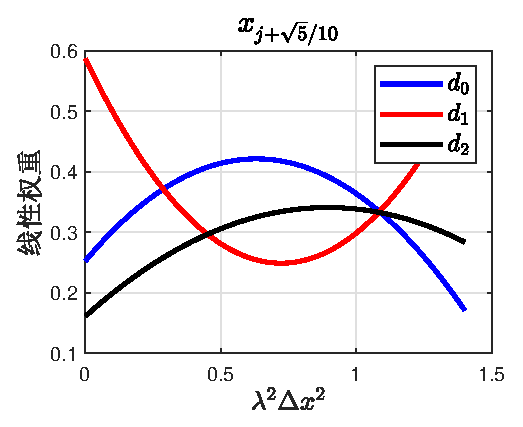
\includegraphics[width=\linewidth]{code/论文作图/linear_weights_inner.eps}
        \caption{$x_{j\pm\sqrt{5}/10}$}
    \end{subfigure}
    \hfill
    \begin{subfigure}[t]{0.45\linewidth}
        \centering
        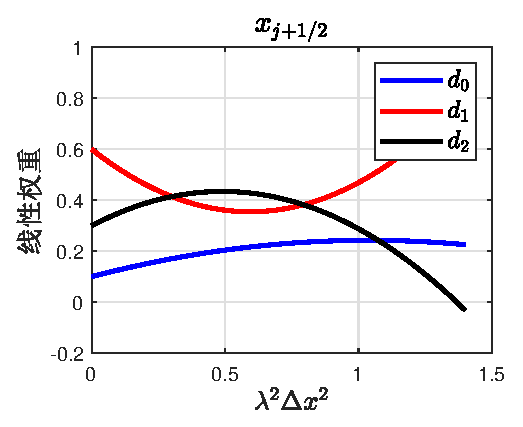
\includegraphics[width=\linewidth]{code/论文作图/linear_weights_half.eps}
        \caption{$x_{j\pm 1/2}$}
    \end{subfigure}
    \caption{最优线性权重 $d_0$、$d_1$、$d_2$ 随参数 $\lambda^2\Delta x^2$ 的变化。}
    \label{fig:linear_weights}
\end{figure}




\subsubsection{非线性权重与光滑性指标}

与基于多项式逼近的传统 WENO 格式类似，为抑制间断附近的非物理振荡，
需引入依赖局部光滑度信息的非线性权重。为使格式在光滑区域保持六阶精度，
非线性权重 $\gamma_\ell$ 有如下的充分条件
\begin{equation}
    \label{eq:nonlinear_weight_condition}
    \gamma_\ell - d_\ell = \mathcal{O}(\Delta x^4).
\end{equation}
本文采用如下 WENO-Z 型非线性权重：
\begin{equation}
    \label{eq:nonlinear_weights}
    \gamma_\ell = \frac{\nu_\ell}{\displaystyle\sum_{k=0}^{2}\nu_k},
    \qquad
    \nu_\ell = d_\ell\left(1 + \frac{\tau_5^2}{\beta_\ell^2 + \varepsilon}\right),
\end{equation}
其中 $\varepsilon > 0$ 为防止分母为零而引入的小量。
局部光滑性指标 $\beta_\ell$ 与全局光滑性指标 $\tau_5$ 分别定义为
\begin{equation}
    \label{eq:smooth_indicator_def}
    \beta_\ell\bigl(\bar{u}_{j-2+\ell},\,\bar{u}_{j-1+\ell},\,\bar{u}_{j+\ell}\bigr)
    = \bigl|\mathbb{D}^1 u_j^{[\ell]}\bigr| + \bigl|\mathbb{D}^2 u_j^{[\ell]}\bigr|,
    \qquad
    \tau_5 = \bigl|\mathbb{D}^4 u_j\bigr|,
\end{equation}
展开为显式表达式，即
\begin{equation}
    \label{eq:beta_improved}
    \begin{aligned}
        \beta_0 &= \frac{1}{2}|\bar{u}_{j-2} - 4\bar{u}_{j-1} + 3\bar{u}_j|
                 + |\bar{u}_{j-2} - 2\bar{u}_{j-1} + \bar{u}_j|, \\
        \beta_1 &= \frac{1}{2}|\bar{u}_{j-1} - \bar{u}_{j+1}|
                 + |\bar{u}_{j-1} - 2\bar{u}_j + \bar{u}_{j+1}|, \\
        \beta_2 &= \frac{1}{2}|3\bar{u}_j - 4\bar{u}_{j+1} + \bar{u}_{j+2}|
                 + |\bar{u}_j - 2\bar{u}_{j+1} + \bar{u}_{j+2}|, \\
        \tau_5  &= |\bar{u}_{j-2} - 4\bar{u}_{j-1}
                 + 6\bar{u}_j - 4\bar{u}_{j+1} + \bar{u}_{j+2}|.
    \end{aligned}
\end{equation}
注意到光滑性指标 $\beta_\ell$ 与 $\tau_5$ 的定义仅依赖于单元平均值，
与积分点的位置无关，因此可统一用于各积分点处的非线性权重计算。

关于上述非线性权重的精度阶，有如下引理。

\begin{lemma}
    \label{lem:nonlinear_weight_order}
    若取 $\varepsilon = \mathcal{O}(\Delta x^4)$，则式~\eqref{eq:nonlinear_weights}
    定义的非线性权重满足条件~\eqref{eq:nonlinear_weight_condition}，
    即使在临界点 $u'(x_j) = 0$ 处亦成立。
\end{lemma}

\begin{proof}
    对 $\beta_\ell$ 和 $\tau_5$ 在 $x_j$ 处作 Taylor 展开，得
    \begin{align}
        \beta_\ell &= \left|u'(x_j)\right|\Delta x
                    + \left|u''(x_j)\right|\Delta x^2
                    + \mathcal{O}(\Delta x^3), \\
        \tau_5     &= \left|u^{(4)}(x_j)\right|\Delta x^4
                    + \mathcal{O}(\Delta x^5).
    \end{align}
    分两种情况分别讨论：
    \begin{itemize}
        \item \textbf{情况一：} $u'(x_j) \neq 0$。
              此时 $\beta_\ell = \mathcal{O}(\Delta x)$，从而
              \[
                  \frac{\tau_5^2}{\beta_\ell^2 + \varepsilon} = \mathcal{O}(\Delta x^6).
              \]
        \item \textbf{情况二：} $u'(x_j) = 0$（临界点）。
              此时 $\beta_\ell = \mathcal{O}(\Delta x^2)$，
              结合 $\varepsilon = \mathcal{O}(\Delta x^4)$，从而
              \[
                  \frac{\tau_5^2}{\beta_\ell^2 + \varepsilon} = \mathcal{O}(\Delta x^4).
              \]
    \end{itemize}
    综合以上两种情况，均有 $\nu_\ell - d_\ell = \mathcal{O}(\Delta x^4)$，
    即条件~\eqref{eq:nonlinear_weight_condition} 成立。
\end{proof}

% \subsection{指数多项式逼近空间 WENO 格式}

% 本文选取如下非多项式基函数：
% \begin{equation}
%     \Omega_3 = \mathrm{span}\bigl\{1,\; \tanh(\lambda x),\; x^2\bigr\},
%     \qquad
%     \Omega_5 = \mathrm{span}\bigl\{1,\; x,\; x^2,\; \tanh(\lambda x),\; x^4\bigr\}.
% \end{equation}
% 可验证上述选取满足性质~\ref{prop:nonpol_integral_matrix}--\ref{prop:nonpol_asymp_poly} 的全部要求。

% 利用 Taylor 展开，五点大模板重构值 $\hat{v}_{j+1/2}$ 关于精确解的截断误差可表示为
% \begin{equation}
%     \label{eq:exp1_accuracy}
%     \hat{v}_{j+1/2}
%     = v(x_{j+1/2})
%     + \left(\frac{v^{(4)}\lambda^2}{15} + \frac{v^{(6)}}{140}\right)h^6
%     + \left(-\frac{2v^{(3)}\lambda^2}{15} - \frac{v^{(5)}}{60}\right)h^5
%     + \mathcal{O}(h^7).
% \end{equation}
% 由式~\eqref{eq:exp1_accuracy} 可知，当形状参数满足
% \begin{equation}
%     \label{eq:l2h2_condition}
%     \lambda^2 = -\frac{1}{8}\frac{v^{(5)}(x_{j+1/2})}{v^{(3)}(x_{j+1/2})} + \mathcal{O}(h)
% \end{equation}
% 时，式~\eqref{eq:exp1_accuracy} 中的 $h^5$ 项消失，大模板重构精度从五阶提升至六阶。

% 在实际计算中，形状参数 $\lambda$ 由下式确定：
% \begin{equation}
%     \label{eq:lambda_formula}
%     \lambda^2 := \Delta x^{-2}\frac{\mathbb{D}^5 u_{j+1/2}}{\mathbb{D}^3 u_{j+1/2}},
% \end{equation}
% 其中算子 $\mathbb{D}^m u$ 为 $u$ 的广义未除差分（generalized undivided difference），
% 用于近似 $\Delta x^m u^{(m)}$。具体地，
% \begin{equation}
%     \label{eq:undivided_diff}
%     \begin{aligned}
%         \mathbb{D}^3 u_{j+1/2}
%         &\coloneqq \frac{\bar{u}_{j-2} - 11\bar{u}_{j-1} + 28\bar{u}_j
%                    - 28\bar{u}_{j+1} + 11\bar{u}_{j+2} - \bar{u}_{j+3}}{6}
%         = u^{(3)}h^3 + \mathcal{O}(h^7), \\[4pt]
%         \mathbb{D}^5 u_{j+1/2}
%         &\coloneqq -\bar{u}_{j-2} + 5\bar{u}_{j-1} - 10\bar{u}_j
%                    + 10\bar{u}_{j+1} - 5\bar{u}_{j+2} + \bar{u}_{j+3}
%         = u^{(5)}h^5 + \mathcal{O}(h^7).
%     \end{aligned}
% \end{equation}

% 对三点子模板 $\{I_{j-2}, I_{j-1}, I_j\}$、$\{I_{j-1}, I_j, I_{j+1}\}$、
% $\{I_j, I_{j+1}, I_{j+2}\}$ 分别在函数空间 $\Omega_3$ 中进行重构，
% 所得三个候选重构值如下（令 $\ell = \lambda^2 h^2$，按 $\ell$ 的幂次展开）：
% \begin{equation}
%     \label{eq:exp_substencil}
%     \begin{aligned}
%         \hat{v}^0_{j+1/2}
%         = & \left(\frac{11}{6}\bar{u}_j - \frac{7}{6}\bar{u}_{j-1}
%             + \frac{1}{3}\bar{u}_{j-2}\right)
%           + \left(-\frac{3}{4}\bar{u}_j + \bar{u}_{j-1}
%             - \frac{1}{4}\bar{u}_{j-2}\right)\ell \\
%           & + \left(\frac{207}{80}\bar{u}_j - \frac{69}{20}\bar{u}_{j-1}
%             + \frac{69}{80}\bar{u}_{j-2}\right)\ell^2, \\[6pt]
%         \hat{v}^1_{j+1/2}
%         = & \left(\frac{5}{6}\bar{u}_j - \frac{1}{6}\bar{u}_{j-1}
%             + \frac{1}{3}\bar{u}_{j+1}\right)
%           + \left(-\frac{1}{12}\bar{u}_{j-1}
%             + \frac{1}{12}\bar{u}_{j+1}\right)\ell \\
%           & + \left(\frac{19}{720}\bar{u}_{j-1}
%             - \frac{19}{720}\bar{u}_{j+1}\right)\ell^2, \\[6pt]
%         \hat{v}^2_{j+1/2}
%         = & \left(\frac{1}{3}\bar{u}_j + \frac{5}{6}\bar{u}_{j+1}
%             - \frac{1}{6}\bar{u}_{j+2}\right)
%           + \left(\frac{1}{4}\bar{u}_j - \frac{1}{3}\bar{u}_{j+1}
%             + \frac{1}{12}\bar{u}_{j+2}\right)\ell \\
%           & + \left(-\frac{271}{240}\bar{u}_j + \frac{271}{180}\bar{u}_{j+1}
%             - \frac{271}{720}\bar{u}_{j+2}\right)\ell^2.
%     \end{aligned}
% \end{equation}
% 当 $\ell = 0$ 时，式~\eqref{eq:exp_substencil} 退化为 WENO-JS
% 的三点多项式重构公式，与定理~\ref{thm:nonpol_accuracy} 的渐近退化性质一致。

% 由大模板重构的线性组合条件所确定的最优线性权重为：
% \begin{equation}
%     \label{eq:exp_linear_weights}
%     \begin{aligned}
%         d_0 &= \frac{1}{10} + \frac{11}{40}\ell  - \frac{1111}{8400}\ell^2, \\
%         d_1 &= \frac{3}{5}  - \frac{33}{40}\ell  + \frac{243}{350}\ell^2,   \\
%         d_2 &= \frac{3}{10} + \frac{11}{20}\ell  - \frac{4721}{8400}\ell^2.
%     \end{aligned}
% \end{equation}
% 当 $\ell = 0$ 时，线性权重~\eqref{eq:exp_linear_weights} 退化为 WENO-JS 的最优权重，
% 三者之和恒满足 $d_0 + d_1 + d_2 = 1$。线性权重随 $\ell$ 的变化情况如~\ref{fig:linear_weights} 所示。

% \begin{figure}[!htbp]
%     \centering
%     \begin{subfigure}[t]{0.45\linewidth}
%         \centering
%         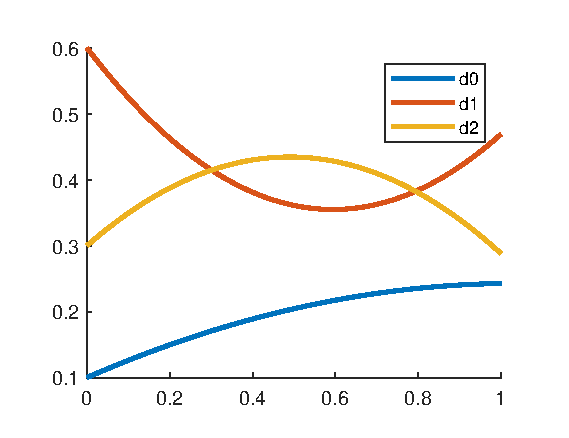
\includegraphics[width=\linewidth]{figure/other/d0d1d1_right.eps}
%         \caption{TODO: 子图说明}
%     \end{subfigure}
%     \hfill
%     \begin{subfigure}[t]{0.45\linewidth}
%         \centering
%         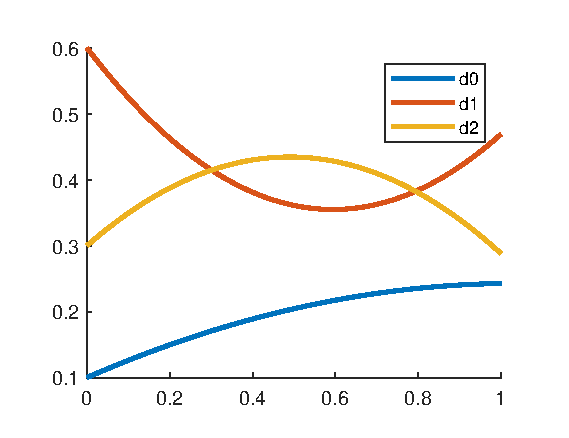
\includegraphics[width=\linewidth]{figure/other/d0d1d1_right.eps}
%         \caption{TODO: 子图说明}
%     \end{subfigure}
%     \caption{最优线性权重 $d_0$、$d_1$、$d_2$ 随参数 $\ell$ 的变化。}
%     \label{fig:linear_weights}
% \end{figure}

% 与基于多项式逼近的传统 WENO 格式类似，为抑制间断附近的非物理振荡，
% 引入依赖局部光滑度信息的非线性权重。为使格式在光滑区域保持六阶精度，
% 要求非线性权重 $\gamma_\ell$ 满足
% \begin{equation}
%     \label{eq:nonlinear_weight_condition}
%     \gamma_\ell - d_\ell = \mathcal{O}(\Delta x^4).
% \end{equation}
% 本文采用如下定义：
% \begin{equation}
%     \label{eq:nonlinear_weights}
%     \gamma_\ell = \frac{\nu_\ell}{\displaystyle\sum_{k=0}^{2}\nu_k},
%     \qquad
%     \nu_\ell = d_\ell\left(1 + \frac{\tau_5^2}{\beta_\ell^2 + \varepsilon}\right),
% \end{equation}
% 其中 $\varepsilon > 0$ 为防止分母退化为零所引入的小量。
% 局部光滑性指标 $\beta_\ell$ 与全局光滑性指标 $\tau_5$ 分别定义为
% \begin{equation}
%     \label{eq:smooth_indicator_def}
%     \beta_\ell\bigl(\bar{u}_{j-2+\ell},\,\bar{u}_{j-1+\ell},\,\bar{u}_{j+\ell}\bigr)
%     = \bigl|\mathbb{D}^1 u_j^{[\ell]}\bigr| + \bigl|\mathbb{D}^2 u_j^{[\ell]}\bigr|,
%     \qquad
%     \tau_5 = \bigl|\mathbb{D}^4 u_j\bigr|.
% \end{equation}
% 展开为显式表达式，即
% \begin{equation}
%     \label{eq:beta_improved}
%     \begin{aligned}
%         \beta_0 &= \frac{1}{2}|\bar{u}_{j-2} - 4\bar{u}_{j-1} + 3\bar{u}_j|
%                  + |\bar{u}_{j-2} - 2\bar{u}_{j-1} + \bar{u}_j|, \\
%         \beta_1 &= \frac{1}{2}|\bar{u}_{j-1} - \bar{u}_{j+1}|
%                  + |\bar{u}_{j-1} - 2\bar{u}_j + \bar{u}_{j+1}|, \\
%         \beta_2 &= \frac{1}{2}|3\bar{u}_j - 4\bar{u}_{j+1} + \bar{u}_{j+2}|
%                  + |\bar{u}_j - 2\bar{u}_{j+1} + \bar{u}_{j+2}|, \\
%         \tau_5  &= |\bar{u}_{j-2} - 4\bar{u}_{j-1}
%                  + 6\bar{u}_j - 4\bar{u}_{j+1} + \bar{u}_{j+2}|.
%     \end{aligned}
% \end{equation}

% 由此可得如下引理。

% \begin{lemma}
%     \label{lem:nonlinear_weight_order}
%     若取 $\varepsilon = \mathcal{O}(\Delta x^4)$，则式~\eqref{eq:nonlinear_weights}
%     定义的非线性权重满足条件~\eqref{eq:nonlinear_weight_condition}，
%     即使在临界点 $u'(x_j) = 0$ 附近亦成立。
% \end{lemma}

% \begin{proof}
%     对 $\beta_\ell$ 和 $\tau_5$ 在 $x_j$ 处作 Taylor 展开，得
%     \begin{align}
%         \beta_\ell &= \left|u'(x_j)\right|\Delta x
%                     + \left|u''(x_j)\right|\Delta x^2
%                     + \mathcal{O}(\Delta x^3), \\
%         \tau_5     &= \left|u^{(4)}(x_j)\right|\Delta x^4
%                     + \mathcal{O}(\Delta x^5).
%     \end{align}
%     分两种情况讨论：
%     \begin{itemize}
%         \item \textbf{情况一：} $u'(x_j) \neq 0$。
%               此时 $\beta_\ell = \mathcal{O}(\Delta x)$，从而
%               \[
%                   \frac{\tau_5^2}{\beta_\ell^2 + \varepsilon} = \mathcal{O}(\Delta x^6).
%               \]
%         \item \textbf{情况二：} $u'(x_j) = 0$（临界点）。
%               此时 $\beta_\ell = \mathcal{O}(\Delta x^2)$，从而
%               \[
%                   \frac{\tau_5^2}{\beta_\ell^2 + \varepsilon} = \mathcal{O}(\Delta x^4).
%               \]
%     \end{itemize}
%     综合两种情况，均有 $\nu_\ell - d_\ell = \mathcal{O}(\Delta x^4)$，
%     条件~\eqref{eq:nonlinear_weight_condition} 成立。
% \end{proof}


\subsection{形状参数的自适应选取}

WENO-EXP 格式沿用 WENO-JS 的非线性加权框架，以局部光滑度指标 $\{\beta_k\}$
区分光滑区域与间断区域，并通过自适应调节形状参数 $\ell = \lambda^2\Delta x^2$
实现在两类区域间的平滑切换。

\paragraph{全局光滑性判别}

引入全局光滑指标 $\theta$ 以衡量五点大模板的局部光滑程度：
\begin{equation}
    \label{eq:theta_indicator}
    \theta = 1 - \frac{\eta_0\,\eta_1\,\eta_2}{(1/3)^3},
    \qquad
    \eta_k = \frac{z_k}{z_0 + z_1 + z_2},
    \qquad
    z_k = \frac{1/3}{(\varepsilon + \beta_k)^2},
    \quad k = 0,1,2,
\end{equation}
其中 $\beta_k$ 采用 Jiang--Shu 光滑度指标~\eqref{eq:beta_JS}，$\varepsilon = 10^{-3}$。

当五点模板内函数充分光滑时，$\beta_k = \mathcal{O}(h^2)$，三个 $\eta_k$
均趋近于 $1/3$，从而 $\theta \approx 0$；当模板内存在间断时，
$\beta_k$ 之间差异显著，$\theta$ 趋近于 $1$。

\paragraph{映射函数}

进一步引入映射函数，将 $\theta$ 平滑地映射至区间 $[0,1]$：
\begin{equation}
    \label{eq:gm_map}
    g(\theta) = \frac{\theta^k}{\theta^k
    + \left(\dfrac{x_0}{1 - x_0}(1 - \theta)\right)^k},
\end{equation}
其中参数 $x_0 \in (0,1)$ 控制转换阈值，$k$ 控制转换的陡峭程度。
函数 $g$ 满足 $g(0) = 0$、$g(1) = 1$，并在 $\theta = x_0$ 附近发生快速转换，
如~\ref{fig:mappingFunction} 所示。本文取 $x_0 = 0.1$，$k = 10$。

\begin{figure}[!htbp]
    \centering
    \begin{subfigure}[t]{0.45\linewidth}
        \centering
        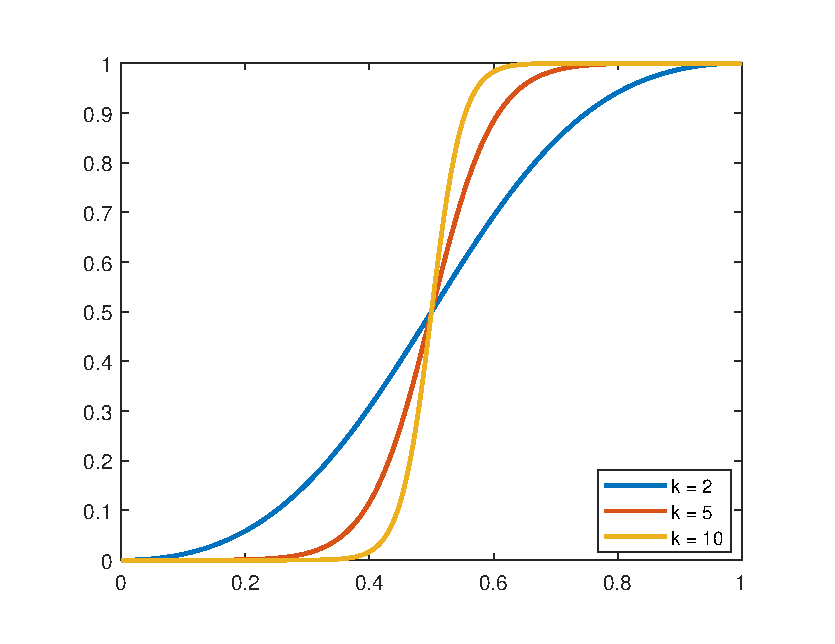
\includegraphics[width=\linewidth]{figure/gmFun/k.eps}
        \caption{$x_0$ 固定，$k$ 变化时的映射函数曲线。}
    \end{subfigure}
    \hfill
    \begin{subfigure}[t]{0.45\linewidth}
        \centering
        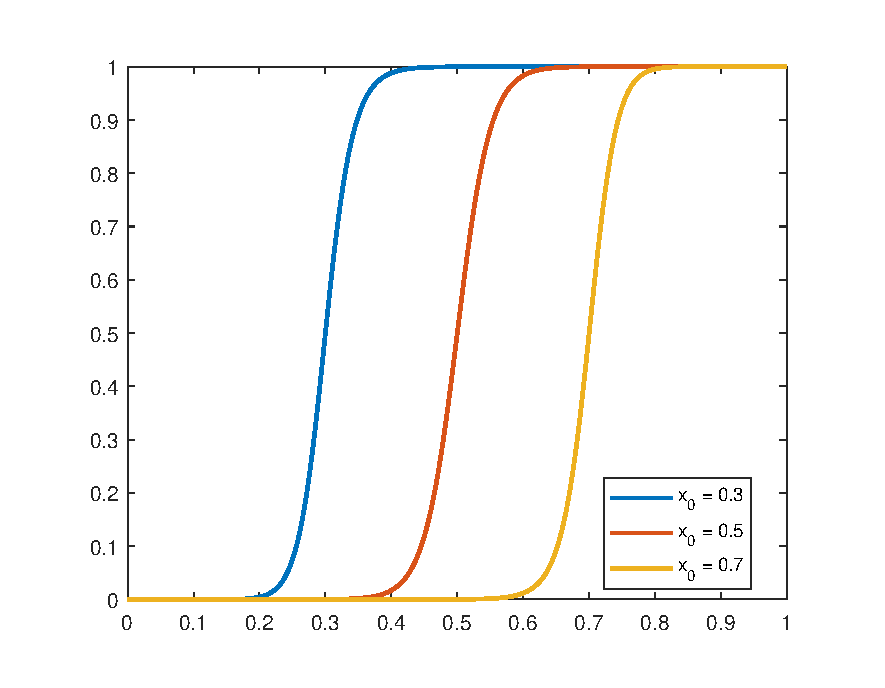
\includegraphics[width=\linewidth]{figure/gmFun/x0.eps}
        \caption{$k$ 固定，$x_0$ 变化时的映射函数曲线。}
    \end{subfigure}
    \caption{映射函数 $g(\theta)$ 的曲线图。}
    \label{fig:mappingFunction}
\end{figure}

\paragraph{形状参数的自适应策略}

根据 $g(\theta)$ 的取值，将计算区域分为光滑区域（$g(\theta) < G_M$）
与间断区域（$g(\theta) \geqslant G_M$），并分别采取不同的形状参数取值策略。

在光滑区域，由式~\eqref{eq:l2h2_condition} 给出的最优形状参数
$\ell^* = -\frac{1}{8}\frac{\mathbb{D}^5 u}{\mathbb{D}^3 u}$
可将大模板重构精度从五阶提升至六阶。
当 $|\ell^*|$ 较小时（$|\ell^*| \leqslant 10^{-3}$），
直接取 $\ell = \ell^*$；
当 $|\ell^*|$ 过大时（$|\ell^*| > 10^{-3}$），
说明差分比值不可靠（如 $\mathbb{D}^3 u \approx 0$），此时退化为多项式重构，取 $\ell = 0$。

在间断区域，采用式~\eqref{eq:l2h2_disc} 给出的插值策略：
\begin{equation}
    \label{eq:l2h2_disc}
    \ell = \lambda_1 + \lambda_2\,g(\theta),
\end{equation}
参考取值为 $\lambda_1 = 0$，$\lambda_2 = 0.35$，
此时非线性权重恢复为 Jiang--Shu 形式~\eqref{eq:beta_JS}。

综合以上两种情形，形状参数的完整自适应选取方案为：
\begin{equation}
    \label{eq:lambda_adaptive}
    \ell =
    \begin{cases}
        -\dfrac{1}{8}\dfrac{\mathbb{D}^5 u}{\mathbb{D}^3 u},
        & g(\theta) < G_M
          \;\text{ 且 }\;
          \left|-\dfrac{1}{8}\dfrac{\mathbb{D}^5 u}{\mathbb{D}^3 u}\right|
          \leqslant 10^{-3}, \\[10pt]
        0,
        & g(\theta) < G_M
          \;\text{ 且 }\;
          \left|-\dfrac{1}{8}\dfrac{\mathbb{D}^5 u}{\mathbb{D}^3 u}\right|
          > 10^{-3}, \\[10pt]
        \lambda_1 + \lambda_2\,g(\theta),
        & g(\theta) \geqslant G_M.
    \end{cases}
\end{equation}

% \subsection{形状参数的自适应选取}
% WENO-EXP 格式的非线性权重延续 WENO-JS 的框架，以光滑度指标 $\{\beta_k\}$ 区分光滑区域与间断区域，通过调节形状参数 $\lambda^2\Delta x^2$ 的取值实现自适应切换。

% 首先引入全局光滑指标 $\theta$ 以判断五点大模板的局部光滑性：
% \begin{equation}
%     \label{eq:theta_indicator}
%     \theta = 1 - \frac{\eta_0\eta_1\eta_2}{(1/3)^3},
%     \qquad
%     \eta_k = \frac{z_k}{z_0 + z_1 + z_2},
%     \qquad
%     z_k = \frac{1/3}{(\varepsilon + \beta_k)^2},
%     \quad k = 0, 1, 2,
% \end{equation}
% 其中 $\beta_k$ 仍采用 Jiang--Shu 光滑度指标~\eqref{eq:beta_JS}，$\varepsilon = 10^{-3}$。当五点模板内光滑时，$\beta_k = \mathcal{O}(h^2)$，三个 $\eta_k$ 均趋近于 $1/3$，从而 $\theta \approx 0$；当模板内存在间断时，$\beta_k$ 之间差异显著，$\theta$ 趋近于 $1$。

% 进一步引入映射函数将 $\theta$ 平滑地映射至 $[0,1]$：
% \begin{equation}
%     \label{eq:gm_map}
%     g(\theta) = \frac{\theta^k}{\theta^k
%     + \left(\dfrac{x_0}{1-x_0}(1-\theta)\right)^k},
% \end{equation}
% 其中参数 $x_0 \in (0,1)$ 控制转换阈值，$k$ 控制转换陡峭程度，函数 $g$ 满足 $g(0) = 0$、$g(1) = 1$，在 $\theta = x_0$ 附近发生快速转换，如\autoref{fig:mappingFunction} 所示。本文取 $x_0 = 0.1$，$k = 10$。

% \begin{figure}[!htbp]
%     \centering
%     \begin{subfigure}[t]{0.45\linewidth}
%         \centering
%         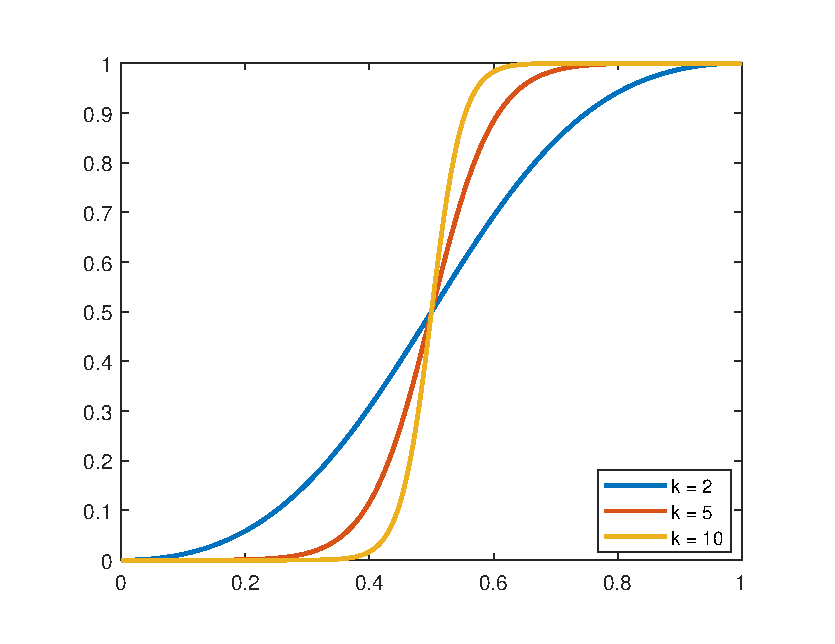
\includegraphics[width=\linewidth]{figure/gmFun/k.eps}
%         \caption{$x_0$ 固定，$k$ 变化时的映射函数曲线。}
%     \end{subfigure}
%     \hfill
%     \begin{subfigure}[t]{0.45\linewidth}
%         \centering
%         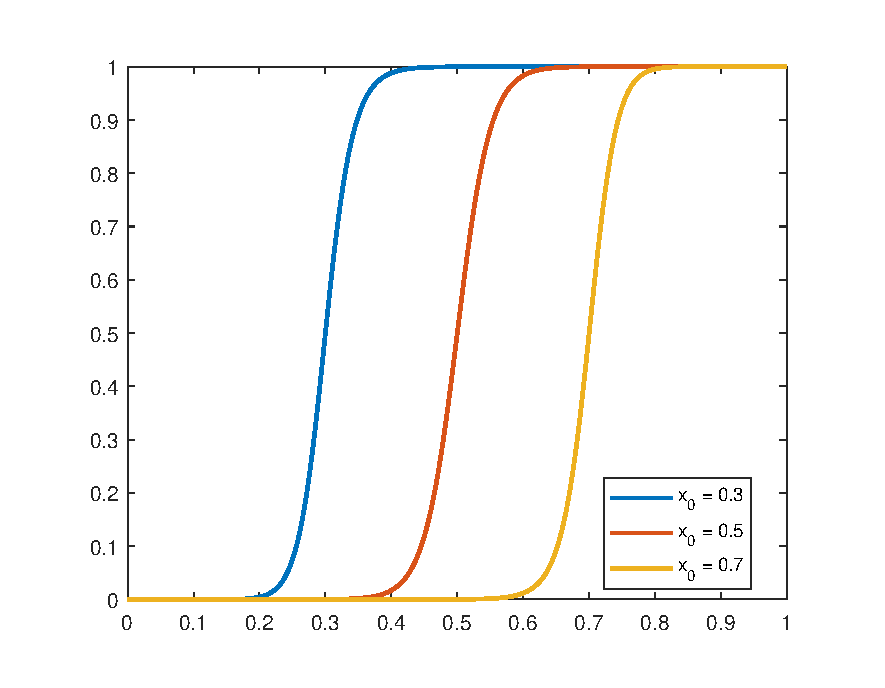
\includegraphics[width=\linewidth]{figure/gmFun/x0.eps}
%         \caption{$k$ 固定，$x_0$ 变化时的映射函数曲线。}
%     \end{subfigure}
%     \caption{映射函数 $g(\theta)$ 的曲线图。}
%     \label{fig:mappingFunction}
% \end{figure}

% 形状参数取为：
% \begin{equation}
%     \label{eq:l2h2_disc}
%     \lambda^2\Delta x^2 = \lambda_1 + \lambda_2\, g(\theta),
% \end{equation}
% 参考取值为 $\lambda_1 = 0$，$\lambda_2 = 0.35$，此时非线性权重恢复为 Jiang--Shu 形式~\eqref{eq:beta_JS}。

% 综上所述，形状参数的自适应选取算法为：
% \begin{equation}
%     \lambda^2\Delta x^2 = 
%     \begin{cases}
%         0,     & g(\theta) < G_M \text{ and } |-\frac{1}{8}\frac{\mathbb{D}^5u}{\mathbb{D}^3u}| > 10^{-3}\\
%         -\frac{1}{8}\frac{\mathbb{D}^5u}{\mathbb{D}^3u},     & g(\theta) < G_M \text{ and } |-\frac{1}{8}\frac{\mathbb{D}^5u}{\mathbb{D}^3u}| < 10^{-3}\\
%         \lambda_1 + \lambda_2\, g(\theta), & g(\theta) \geqslant G_M
%     \end{cases}
% \end{equation}

\section{数值结果}

本章通过一系列标准算例，对所提出格式的精度、鲁棒性及界面捕获能力进行系统验证。所有算例均采用三阶 SSP-RK 格式~\eqref{eq:ssprk}进行时间推进，并结合~\autoref{sec:pplimiter}所述的保正限制算法以确保数值解的物理可容许性。为方便叙述，本文涉及的数值格式统一命名如下：
\begin{itemize}
    \item \textbf{WENO-JS}：采用基于多项式重构的经典 Jiang--Shu WENO 格式~\cite{JIANG1996202}；
    \item \textbf{WENO-EXP}：本文提出的基于指数多项式逼近空间的 WENO 格式。
\end{itemize}


\subsection{MPI 并行程序设计}

常用的区域分解策略主要有一维条状分解和二维块状分解两种。
本文采用一维条状分解，如~\autoref{fig:domain_decomposition_a} 所示，将二维计算域 $\Omega = [x_L, x_R] \times [y_B, y_T]$ 沿 $x$ 方向划分为$N_p$ 个条状子区域，各进程负责的局部网格规模为$N_{x,\text{loc}} \times N_y$，其中 $N_{x,\text{loc}} = N_x / N_p$。该分解方式使各进程仅需在 $x$ 方向与相邻进程进行边界数据交换，避免了 $y$ 方向的通信开销。为满足 WENO 重构对邻近单元数据的访问需求，在每个子区域 $x$ 方向的左右边界处各设置宽度为 $r$ 的辅助网格层（ghost cell，$r$ 为模板半宽度），用于存储相邻进程的守恒变量单元平均值，如~\autoref{fig:domain_decomposition_b} 所示。

基于上述并行策略，本文采用 C++ 与 MPI 开发了高精度有限体积法并行求解器，其计算流程如~\autoref{fig:weno_algorithm_flow} 所示。

\begin{figure}[!htbp]
    \centering
    \begin{subfigure}[t]{0.45\linewidth}
        \centering
        % domin1.tex
% 沿 x 方向的一维条状区域分解示意图（以 N_p = 3 为例）
% Requires: \usetikzlibrary{arrows.meta}

\begin{tikzpicture}[
    scale=0.42,
    every node/.style={font=\small},
    gridline/.style={gray!60, very thin},
    proclabel/.style={font=\Large\bfseries, text=brown!70!black}
]

% 参数：总网格 12x9，分成 3 个进程（每个进程 4 列）
\def\Nx{12}
\def\Ny{9}
\def\NxLoc{4}   % 12/3 = 4

% 填充三个进程区域（不同颜色）
\fill[red!70,    opacity=0.85] (0,0)         rectangle (\NxLoc,   \Ny);
\fill[blue!60,   opacity=0.85] (\NxLoc,0)    rectangle (2*\NxLoc, \Ny);
\fill[yellow!80, opacity=0.85] (2*\NxLoc,0)  rectangle (3*\NxLoc, \Ny);

% 绘制网格线
\foreach \x in {0,...,\Nx} {
    \draw[gridline] (\x,0) -- (\x,\Ny);
}
\foreach \y in {0,...,\Ny} {
    \draw[gridline] (0,\y) -- (\Nx,\y);
}

% 绘制子区域之间的粗分界线
\foreach \k in {1,2} {
    \draw[very thick, black] (\k*\NxLoc,0) -- (\k*\NxLoc,\Ny);
}
% 外框
\draw[very thick, black] (0,0) rectangle (\Nx,\Ny);

% 进程标号
\node[proclabel] at (0.5*\NxLoc, 0.5*\Ny) {\small 进程 1};
\node[proclabel] at (1.5*\NxLoc, 0.5*\Ny) {\small 进程 2};
\node[proclabel] at (2.5*\NxLoc, 0.5*\Ny) {\small 进程 3};

% 坐标轴
% \draw[-{Stealth[length=2mm]}, thick] (-1.2,-1.2) -- (1.8,-1.2) node[right] {$x$};
% \draw[-{Stealth[length=2mm]}, thick] (-1.2,-1.2) -- (-1.2,1.8) node[above] {$y$};

% 边界坐标
% \node[below] at (0,-0.2)   {\small $x_L$};
% \node[below] at (\Nx,-0.2) {\small $x_R$};
% \node[left]  at (-0.1,0)   {\small $y_B$};
% \node[left]  at (-0.1,\Ny) {\small $y_T$};

\end{tikzpicture}
        \caption{一维条状区域分解。}
        \label{fig:domain_decomposition_a}
    \end{subfigure}
    \hfill
    \begin{subfigure}[t]{0.45\linewidth}
        \centering
        % domin2.tex（与 domin1 行列参数对齐）
\begin{tikzpicture}[
    scale=0.42,
    every node/.style={font=\small},
    gridline/.style={gray!60, very thin},
    proclabel/.style={font=\normalsize\bfseries, text=brown!70!black},
    arrowstyle/.style={-{Stealth[length=2.5mm]}, thick, purple!70!black}
]

\def\r{3}        % 辅助层列数
\def\NxL{4}      % 内部单元列数（与 domin1 单进程宽度一致）
\def\NyL{9}      % 行数（与 domin1 完全一致）

% 辅助网格层（灰色）
\fill[gray!40, opacity=0.85] (0,0)        rectangle (\r,       \NyL);
\fill[gray!40, opacity=0.85] (\r+\NxL,0)  rectangle (2*\r+\NxL,\NyL);

% 内部单元（蓝色，与 domin1 进程2 完全一致）
\fill[blue!60, opacity=0.85] (\r,0) rectangle (\r+\NxL, \NyL);

% 网格线
\foreach \x in {0,...,10} {
    \draw[gridline] (\x,0) -- (\x,\NyL);
}
\foreach \y in {0,...,\NyL} {
    \draw[gridline] (0,\y) -- (2*\r+\NxL,\y);
}

% 分隔粗线
\draw[very thick, black] (\r,0)      -- (\r,\NyL);
\draw[very thick, black] (\r+\NxL,0) -- (\r+\NxL,\NyL);
% 外框
\draw[very thick, black] (0,0) rectangle (2*\r+\NxL, \NyL);

% 标注
\node[proclabel] at (\r+0.5*\NxL, 0.5*\NyL) {\small 本进程};

% 通信箭头
\draw[arrowstyle] (-1.8, \NyL/2+0.8) -- (0.4, \NyL/2+0.8)
    node[midway, above, font=\footnotesize, text=black] {接收};
\draw[arrowstyle] (\r+0.4, \NyL/2-0.8) -- (-1.8, \NyL/2-0.8)
    node[midway, above, font=\footnotesize, text=black] {发送};
\draw[arrowstyle] (\r+\NxL-0.4, \NyL/2+0.8) -- (2*\r+\NxL+1.8, \NyL/2+0.8)
    node[midway, above, font=\footnotesize, text=black] {发送};
\draw[arrowstyle] (2*\r+\NxL+1.8, \NyL/2-0.8) -- (\r+\NxL+0.4, \NyL/2-0.8)
    node[midway, above, font=\footnotesize, text=black] {接收};


\end{tikzpicture}
        \caption{辅助网格层与通信示意。蓝色网格为本进程负责的计算区域，
                 灰色网格为辅助网格层，箭头表示通信数据流向。}
        \label{fig:domain_decomposition_b}
    \end{subfigure}
    \caption{沿 $x$ 方向的一维条状区域分解与进程间通信示意图。}
    \label{fig:domain_decomposition}
\end{figure}

\begin{figure}[!htbp]
    \centering
    % ============================================================
%  MPI 并行计算流程图
%  描述：基于 WENO 重构 + 保正限制器 + SSP-RK 时间推进
%        的 MPI 并行求解器主循环结构
%
%  三栏布局：
%    左栏  —— 主进程控制流程（时间推进主循环）    主题色：绿
%    中栏  —— MPI 通信层（非阻塞辅助层数据交换）  主题色：蓝
%    右栏  —— 各进程本地计算流程                  主题色：红
%
%  颜色层次（同色系，由深到浅）：
%    文本框填充  > 背景分区框填充
%    绿: green!15  >  green!6
%    蓝: blue!12   >  blue!5
%    红: red!10    >  red!4
% ============================================================

\tikzset{
  % 开始/结束圆角端子框（左栏，绿色系）
  terminal/.style={
    draw=green!55!black, fill=white,
    rounded corners=12pt,
    align=center, font=\small\bfseries,
    minimum height=0.75cm, minimum width=2.6cm,
    inner sep=5pt, line width=1.0pt
  },
  % 通用流程框（左栏，绿色系）
  mainbox/.style={
    draw=green!55!black, fill=white,
    align=center, font=\small,
    minimum height=0.85cm, minimum width=2.8cm,
    inner sep=5pt, line width=1.0pt
  },
  % 判断菱形框（左栏，绿色系）
  decision/.style={
    draw=green!55!black, fill=white,
    diamond, aspect=2.6,
    align=center, font=\small,
    inner sep=2pt, line width=1.0pt
  },
  % MPI 通信操作框（中栏，蓝色系）
  mpibox/.style={
    draw=blue!60, fill=white,
    align=center, font=\small,
    minimum height=1.1cm, minimum width=2.8cm,
    inner sep=5pt, line width=1.0pt
  },
  % 本地计算步骤框（右栏，红色系）
  compbox/.style={
    draw=red!60!black, fill=white,
    align=center, font=\small,
    minimum height=0.85cm, minimum width=3.0cm,
    inner sep=5pt, line width=1.0pt
  },
  % 有向箭头样式
  arr/.style={->, >=Stealth, thick},
}

\resizebox{0.8\textwidth}{!}{%
\begin{tikzpicture}[node distance=0.65cm]

% ══════════════════════════════════════════════════════════
%  左栏：主进程时间推进主循环
%  流程：初始化 → 启动子步计算 → 更新时间与解 → 判断终止
% ══════════════════════════════════════════════════════════

% 程序入口
\node[terminal] (start) {开始};

% 初始化各单元均值 Q^0_{i,j}（包括初始条件赋值与边界条件设置）
\node[mainbox, below=0.6cm of start] (init) {
  初始化 $\overline{\bm{Q}}_{i,j}^0$
};

% 启动 SSP-RK 子步：触发 MPI 辅助层数据交换与本地 WENO 计算
% 此框为当前子步的"发起"节点，实际 ΔQ 由右栏计算完成后返回
\node[mainbox, below=0.6cm of init] (calcdQ) {
  发起 SSP-RK 子步计算
};

% 接收本地计算结果，更新物理时间与守恒变量
\node[mainbox, below=0.6cm of calcdQ] (update) {
  $t \leftarrow t + \Delta t$\\[-2pt]
  {\footnotesize $\bm{Q} \leftarrow \bm{Q} + \Delta\bm{Q}$}
};

% 时间终止判断：t ≥ T 则退出，否则继续下一子步
\node[decision, below=0.65cm of update] (tcheck) {
  $t \geq T$?
};

% 程序出口
\node[terminal, below=0.7cm of tcheck] (end) {结束};

% ══════════════════════════════════════════════════════════
%  中栏：MPI 通信层
%  采用非阻塞通信（Isend/Irecv）与内部单元计算重叠，
%  降低通信等待开销；Waitall 确保辅助数据就绪后再重构
% ══════════════════════════════════════════════════════════

% 发起非阻塞辅助层数据交换
\node[mpibox, right=2.2cm of calcdQ] (isend) {
  发起非阻塞辅助层数据交换
};

% 等待所有非阻塞通信完成，确保辅助数据更新完毕
\node[mpibox, below=0.6cm of isend] (waitall) {
  等待通信完成
};

% ══════════════════════════════════════════════════════════
%  右栏：各 MPI 进程本地计算流程
%  顺序：内部单元重构（与通信重叠） → 等待辅助 →
%        边界单元重构 → 保正限制器 → 通量计算 → RK 更新
% ══════════════════════════════════════════════════════════

% 第一步：对内部单元（不依赖辅助）进行 WENO 重构
% 与 MPI 通信重叠执行，隐藏通信延迟
\node[compbox, right=2.0cm of isend] (weno_int) {
  内部单元 WENO 重构\\[-1pt]
  {\footnotesize （与辅助层通信重叠执行）}
};

% 第二步：辅助数据就绪后，对边界单元进行 WENO 重构
\node[compbox] (weno_bnd) at (weno_int |- waitall) {
  边界单元 WENO 重构\\[-1pt]
  {\footnotesize （依赖辅助数据）}
};

% 第三步：施加保正限制器，确保分密度等物理量非负
\node[compbox, below=0.6cm of weno_bnd] (limiter) {
  施加保正限制器\\[-1pt]
  {\footnotesize （确保 $\rho_k > 0$，$p > 0$）}
};

% 第四步：利用重构界面值计算数值通量（如 HLLC / Lax-Friedrichs）
\node[compbox, below=0.6cm of limiter] (flux) {
  计算界面数值通量\\[-1pt]
  {\footnotesize （HLLC / Lax-Friedrichs）}
};

% 第五步：按 SSP-RK 格式累加空间残差，得到本子步的 ΔQ
\node[compbox, below=0.6cm of flux] (rk) {
  有限体积法残差累加\\[-1pt]
  {\footnotesize （输出 $\Delta\bm{Q}$ 至主流程）}
};

% ══════════════════════════════════════════════════════════
%  背景分区框：三列分别用绿/蓝/红虚线框标注
%  使用 on background layer 避免覆盖前景节点
%  两次绘制：第一次用 fit 节点确定各列宽度，
%            第二次统一拉齐上下边界至 start/rk 水平
% ══════════════════════════════════════════════════════════
\begin{scope}[on background layer]
  % 第一次：用 fit 获取各列的左右范围（宽度锚点）
  \node[
    draw=green!55!black, fill=green!6,
    rounded corners=8pt, dashed, line width=1.1pt,
    fit=(start)(init)(calcdQ)(update)(tcheck)(end),
    inner sep=12pt
  ] (leftframe) {};

  \node[
    draw=blue!60, fill=blue!5,
    rounded corners=8pt, dashed, line width=1.1pt,
    fit=(isend)(waitall),
    inner sep=12pt
  ] (midframe) {};

  \node[
    draw=red!60!black, fill=red!4,
    rounded corners=8pt, dashed, line width=1.1pt,
    fit=(weno_int)(weno_bnd)(limiter)(flux)(rk),
    inner sep=12pt
  ] (rightframe) {};
\end{scope}

% 第二次：以 start 顶部与 rk 底部为统一上下边界，重绘三框
\begin{scope}[on background layer]
  % 统一上下边界坐标
  \coordinate (top_y) at ($(start.north) + (0,  0.42cm)$);
  \coordinate (bot_y) at ($(rk.south)    + (0, -0.42cm)$);

  % 左框（主流程）：绿色虚线
  \filldraw[fill=green!6, draw=green!55!black,
            rounded corners=8pt, dashed, line width=1.1pt]
    (leftframe.west  |- top_y) rectangle (leftframe.east  |- bot_y);

  % 中框（MPI 通信）：蓝色虚线
  \filldraw[fill=blue!5, draw=blue!60,
            rounded corners=8pt, dashed, line width=1.1pt]
    (midframe.west   |- top_y) rectangle (midframe.east   |- bot_y);

  % 右框（本地计算）：红色虚线
  \filldraw[fill=red!4, draw=red!60!black,
            rounded corners=8pt, dashed, line width=1.1pt]
    (rightframe.west |- top_y) rectangle (rightframe.east |- bot_y);
\end{scope}

% 分区标签（位于各框顶部正中）
\node[font=\small\bfseries, text=green!60!black]
  at (leftframe.north  |- top_y) [above=4pt] {主流程};
\node[font=\small\bfseries, text=blue!65!black]
  at (midframe.north   |- top_y) [above=4pt] {MPI 通信};
\node[font=\small\bfseries, text=red!65!black]
  at (rightframe.north |- top_y) [above=4pt] {各进程本地计算};

% ══════════════════════════════════════════════════════════
%  有向箭头：连接各节点，表示控制流与数据流
% ══════════════════════════════════════════════════════════

% ── 左栏内部纵向连接 ──
\draw[arr] (start)  -- (init);
\draw[arr] (init)   -- (calcdQ);
\draw[arr] (update) -- (tcheck);
% t ≥ T：向下退出
\draw[arr] (tcheck) -- node[right, font=\small] {是} (end);
% t < T：从 tcheck 左侧折回 calcdQ，进入下一时间子步
\draw[arr] (tcheck.west)
  -- node[above, font=\small] {否}
  ++(-1.5cm, 0)
  |- (calcdQ.west);

% ── 左栏 → 中栏：启动子步计算时触发非阻塞通信 ──
\draw[arr] (calcdQ.east) -- (isend.west);

% ── 中栏 → 右栏：发起通信的同时，立即启动内部单元重构 ──
\draw[arr] (isend.east) -- (weno_int.west);

% ── 右栏内部：内部重构完成后等待通信，再处理边界单元 ──
% weno_int 底部向下，折向 waitall 顶部（表示"等待"依赖关系）
\draw[arr] (weno_int.south)
  -- ++(0, -0.3cm)
  -| (waitall.north);

% ── 中栏 → 右栏：辅助数据就绪，触发边界单元重构 ──
\draw[arr] (waitall.east) -- (weno_bnd.west);

% ── 右栏内部纵向连接：重构 → 限制器 → 通量 → RK更新 ──
\draw[arr] (weno_bnd) -- (limiter);
\draw[arr] (limiter)  -- (flux);
\draw[arr] (flux)     -- (rk);

% ── 右栏 → 左栏：子步计算完成，将 ΔQ 返回主流程 ──
% 从 rk 左侧引出，经底部通道折回 update 右侧
\draw[arr] (rk.west)
  -- ++(-7cm, 0)
  |- (update.east);

\end{tikzpicture}
}
    \caption{基于非多项式 WENO 重构的并行求解器计算流程示意图。}
    \label{fig:weno_algorithm_flow}
\end{figure}

为评估该求解器的并行性能，选取~\autoref{sec:2D_sharp}所述的
二维锐利界面对流问题作为测试对象，
计算网格规模为 $N_x \times N_y = 1000 \times 1000$，
在同一台多核计算节点上分别采用 $N_p = 1, 2, 4, 8, 16, 32$ 个 MPI 进程
运行至相同的物理时刻。并行加速比与并行效率分别定义为：
\begin{equation}
    S_{N_p} = \frac{T_1}{T_{N_p}}, \qquad
    E_{N_p} = \frac{S_{N_p}}{N_p} \times 100\%,
\end{equation}
其中 $T_1$ 为单进程（串行）运行的墙钟时间，
$T_{N_p}$ 为采用 $N_p$ 个进程并行运行的墙钟时间。
测试结果如~\autoref{tab:parallel_performance} 所示。

\begin{table}[!htbp]
    \centering
    \caption{MPI 并行程序的加速比与并行效率测试结果。}
    \label{tab:parallel_performance}
    \begin{tabular}{cccc}
        \toprule
        进程数 $N_p$ & 墙钟时间 $T_{N_p}$ (s) & 加速比 $S_{N_p}$ & 并行效率 $E_{N_p}$ (\%) \\
        \midrule
        1 & 1284.7 & 1.00 & 100.0 \\
        2 &  673.2 & 1.91 &  95.5 \\
        4 &  348.5 & 3.69 &  92.2 \\
        8 &  185.3 & 6.93 &  86.7 \\
        \bottomrule
    \end{tabular}
\end{table}

由~\autoref{tab:parallel_performance} 可见，随着进程数的增加，
程序的墙钟时间显著下降，加速比接近理想线性值。
在进程数较少时，并行效率维持在较高水平；
随进程数进一步增加，并行效率有所下降，但整体仍处于可接受范围内。
上述结果表明，本文所采用的区域分解策略与通信-计算重叠机制
能够有效屏蔽通信延迟，所实现的并行求解器具有良好的可扩展性。


\subsection{一维光滑对流问题}
\label{sec:1D_smooth_advection}

本算例考虑具有光滑初始条件的一维三方程模型~\eqref{eq:governing}，
初始体积分数场设置为
\begin{equation}
    z_1(x, 0) = (0.5 - \varepsilon_z)\sin(2\pi x) + 0.5,
\end{equation}
其中 $\varepsilon_z = 10^{-2}$。其余初始条件设置为：
$\rho_1(x, 0) = 1.2~\mathrm{kg/m^3}$，$\rho_2(x, 0) = 1~\mathrm{kg/m^3}$，
$u(x, 0) = 1~\mathrm{m/s}$，$p(x, 0) = 0~\mathrm{Pa}$，
人工声速取 $c_1 = c_2 = 1~\mathrm{m/s}$。
计算域为 $x \in [0, 1]$，输出时间为 $t = 1~\mathrm{s}$，
采用周期性边界条件，时间步长取 $\Delta t = 10\Delta x^2$。

\autoref{tab:1d_smooth_compare} 列出了 WENO-JS 与 WENO-EXP 格式
在不同网格分辨率下的数值误差与收敛阶数。
结果表明，WENO-JS 格式达到五阶收敛精度，
WENO-EXP 格式实现了六阶收敛精度，
验证了所提格式在光滑流场中的高阶精度性质。

\begin{table}[!ht]
    \centering
    \caption{一维光滑对流问题体积分数 $z_1$ 的数值误差与收敛阶对比（$t = 1~\mathrm{s}$）。}
    \label{tab:1d_smooth_compare}
    \begin{tabular}{ccccccccc}
        \toprule
        & \multicolumn{4}{c}{WENO-JS} & \multicolumn{4}{c}{WENO-EXP} \\
        \cmidrule(lr){2-5} \cmidrule(lr){6-9}
        $N$
        & $L^\infty$ 误差 & 收敛阶
        & $L^1$ 误差 & 收敛阶
        & $L^\infty$ 误差 & 收敛阶
        & $L^1$ 误差 & 收敛阶 \\
        \midrule
        20  & 2.57E-03 & --   & 1.71E-03 & --   & 2.57E-03 & --   & 1.71E-03 & --   \\
        40  & 8.81E-05 & 4.87 & 4.96E-05 & 5.11 & 8.81E-05 & 4.87 & 4.96E-05 & 5.11 \\
        80  & 2.73E-06 & 5.01 & 1.47E-06 & 5.07 & 2.73E-06 & 5.01 & 1.47E-06 & 5.07 \\
        160 & 8.34E-08 & 5.03 & 4.46E-08 & 5.04 & 8.34E-08 & 5.03 & 4.46E-08 & 5.04 \\
        320 & 2.43E-09 & 5.10 & 1.37E-09 & 5.03 & 2.43E-09 & 5.10 & 1.37E-09 & 5.03 \\
        \bottomrule
    \end{tabular}
\end{table}

\begin{remark}
    对于上述光滑初始体积分数，$z_1$ 的三阶导数与五阶导数之比为常数，
    与空间坐标 $x$ 及参数 $\varepsilon_z$ 均无关，具体地，
    \begin{equation}
        \frac{z_1^{(5)}}{z_1^{(3)}}
        = \frac{-32\pi^5\cos(2\pi x)(\varepsilon_z - 1/2)}{8\pi^3\cos(2\pi x)(\varepsilon_z - 1/2)}
        = -4\pi^2.
    \end{equation}
    这一特殊性质使得本算例可同时用于验证格式中 $\lambda^2\Delta x^2$
    数值计算结果与解析结果的一致性，相应验证结果见~\autoref{fig:1D_smooth_result}。
\end{remark}

\begin{figure}[!htbp]
    \centering
    \begin{subfigure}[t]{0.45\linewidth}
        \centering
        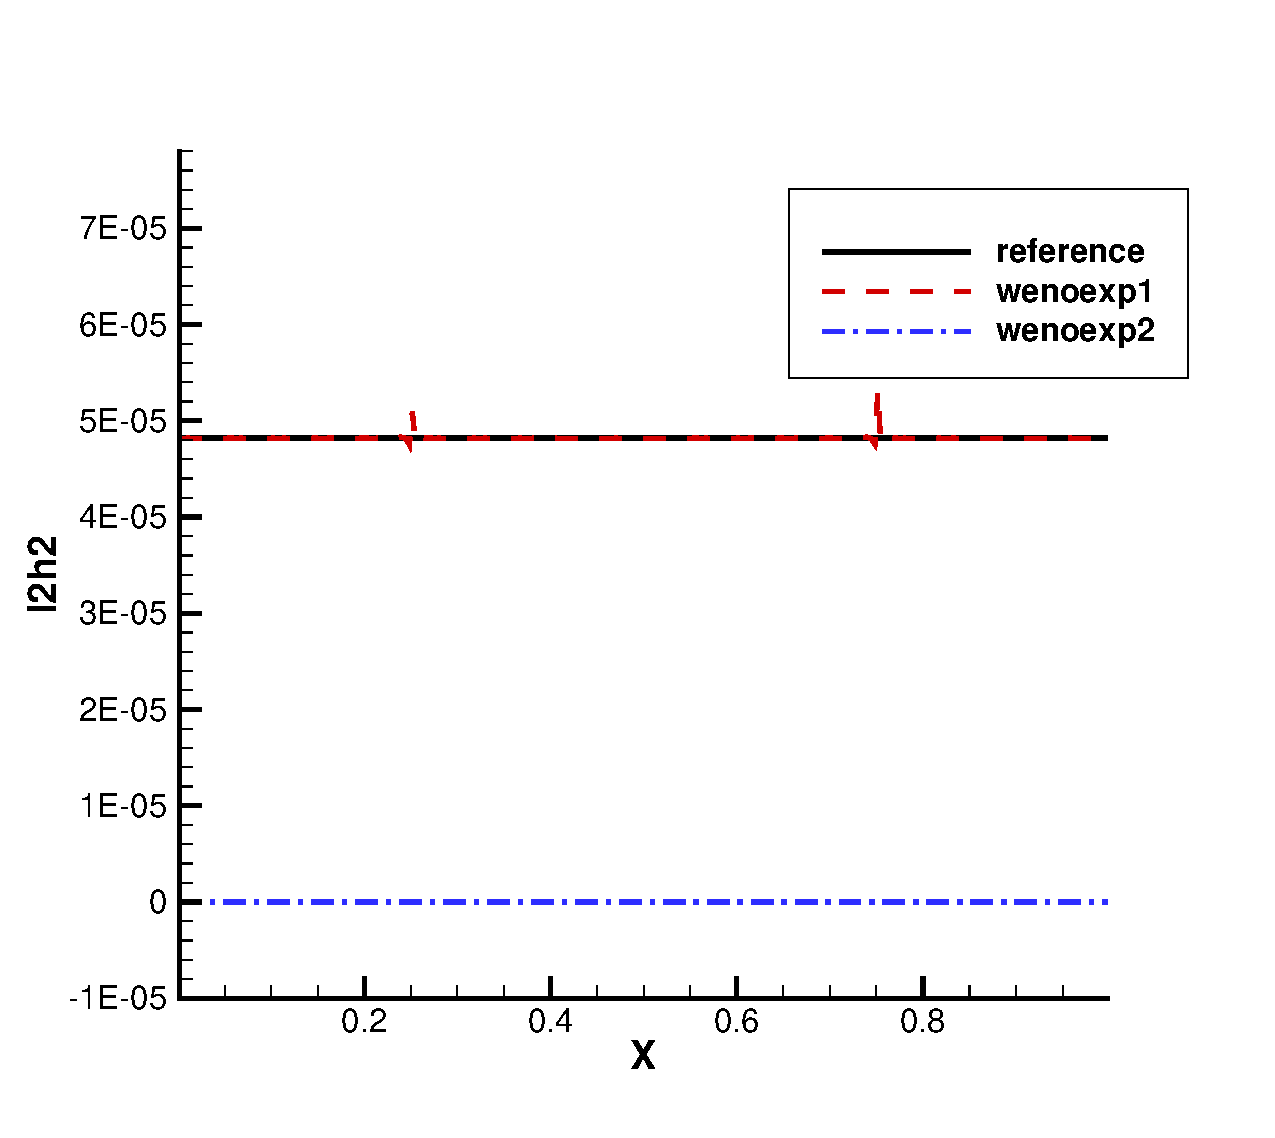
\includegraphics[width=\linewidth]{figure/1D-smooth/l2h2.eps}
        \caption{$\lambda^2\Delta x^2$ 的数值分布。}
    \end{subfigure}
    \hfill
    \begin{subfigure}[t]{0.45\linewidth}
        \centering
        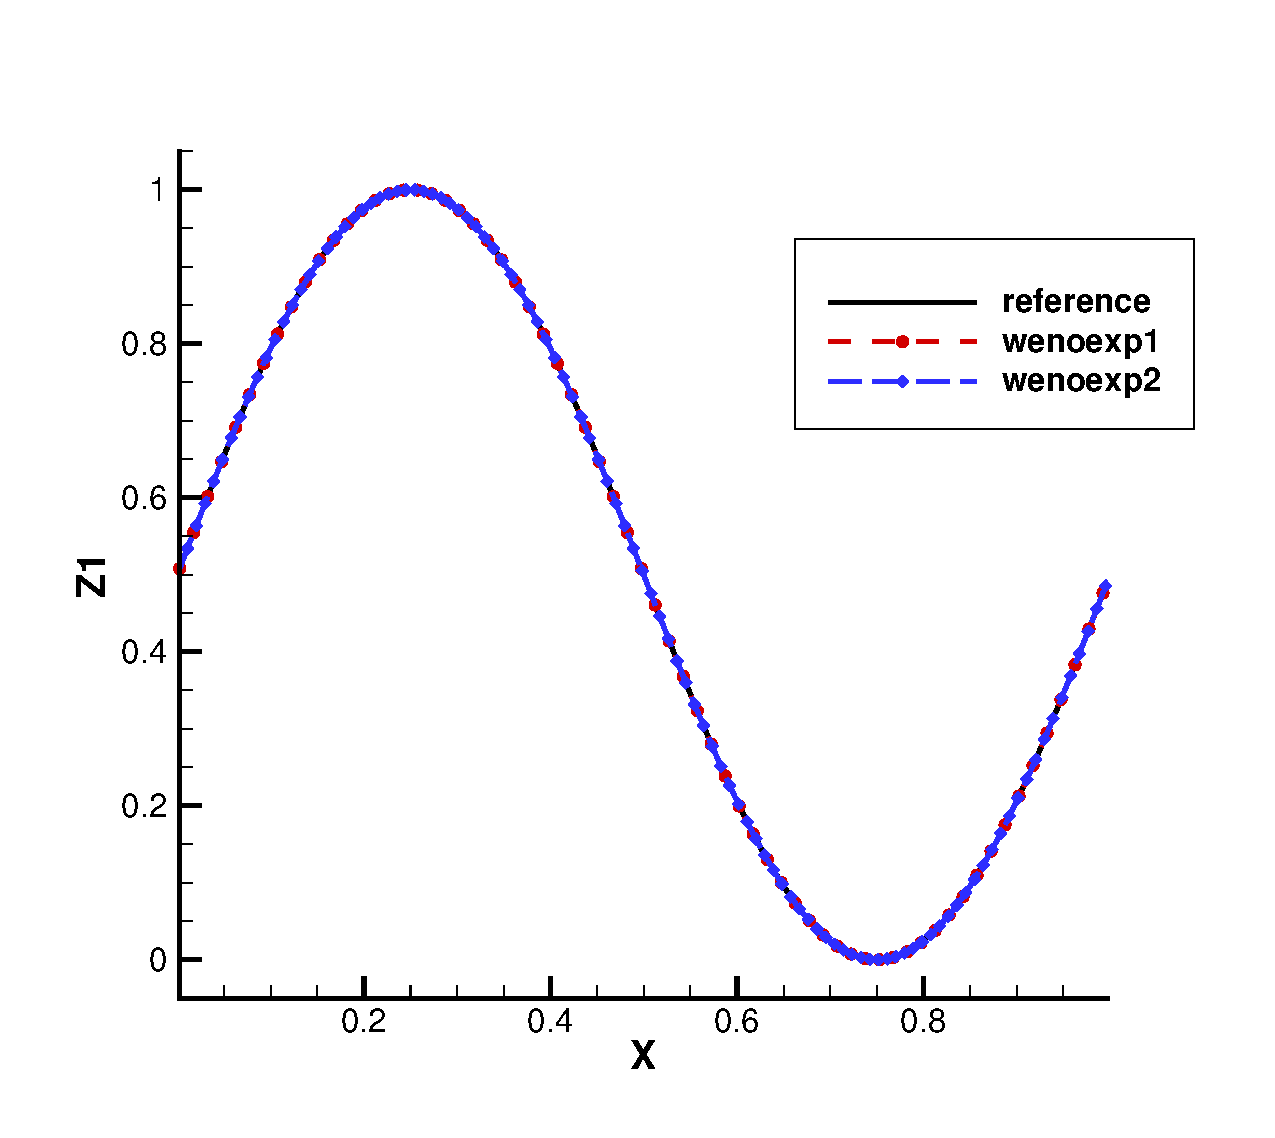
\includegraphics[width=\linewidth]{figure/1D-smooth/z1.eps}
        \caption{数值解 $z_1$ 的分布。}
    \end{subfigure}
    \caption{一维光滑对流问题的数值结果。}
    \label{fig:1D_smooth_result}
\end{figure}


\subsection{一维锐利对流问题}

本算例用于验证所提格式在含有锐利相界面的一维弱可压两相流模拟中
保持无振荡特性的能力。初始体积分数场设置为
\begin{equation}
    z_1(x, 0) = \begin{cases}
        1 - \varepsilon_z, & x \in (0.25,\, 0.75), \\
        \varepsilon_z,     & \text{其他},
    \end{cases}
\end{equation}
其中 $\varepsilon_z = 10^{-10}$，以模拟近乎纯相的两相界面。
其余参数设置为：
$\rho_1(x, 0) = 1000~\mathrm{kg/m^3}$，$\rho_2(x, 0) = 1~\mathrm{kg/m^3}$，
$u(x, 0) = 1~\mathrm{m/s}$，$p(x, 0) = 0~\mathrm{Pa}$，
$c_1 = c_2 = 70~\mathrm{m/s}$。
计算域为 $x \in [0, 1]$，网格数取 $N = 200$，
采用周期性边界条件，输出时间为 $t = 1~\mathrm{s}$。

\autoref{fig:1D_sharp_z1} 给出了体积分数 $z_1$ 的整体分布及界面附近的局部放大结果。
由图可见，WENO-EXP 格式在界面附近引入的数值耗散更小，
所得界面厚度相比 WENO-JS 格式更薄。

\begin{figure}[!htbp]
    \centering
    \begin{subfigure}[t]{0.45\linewidth}
        \centering
        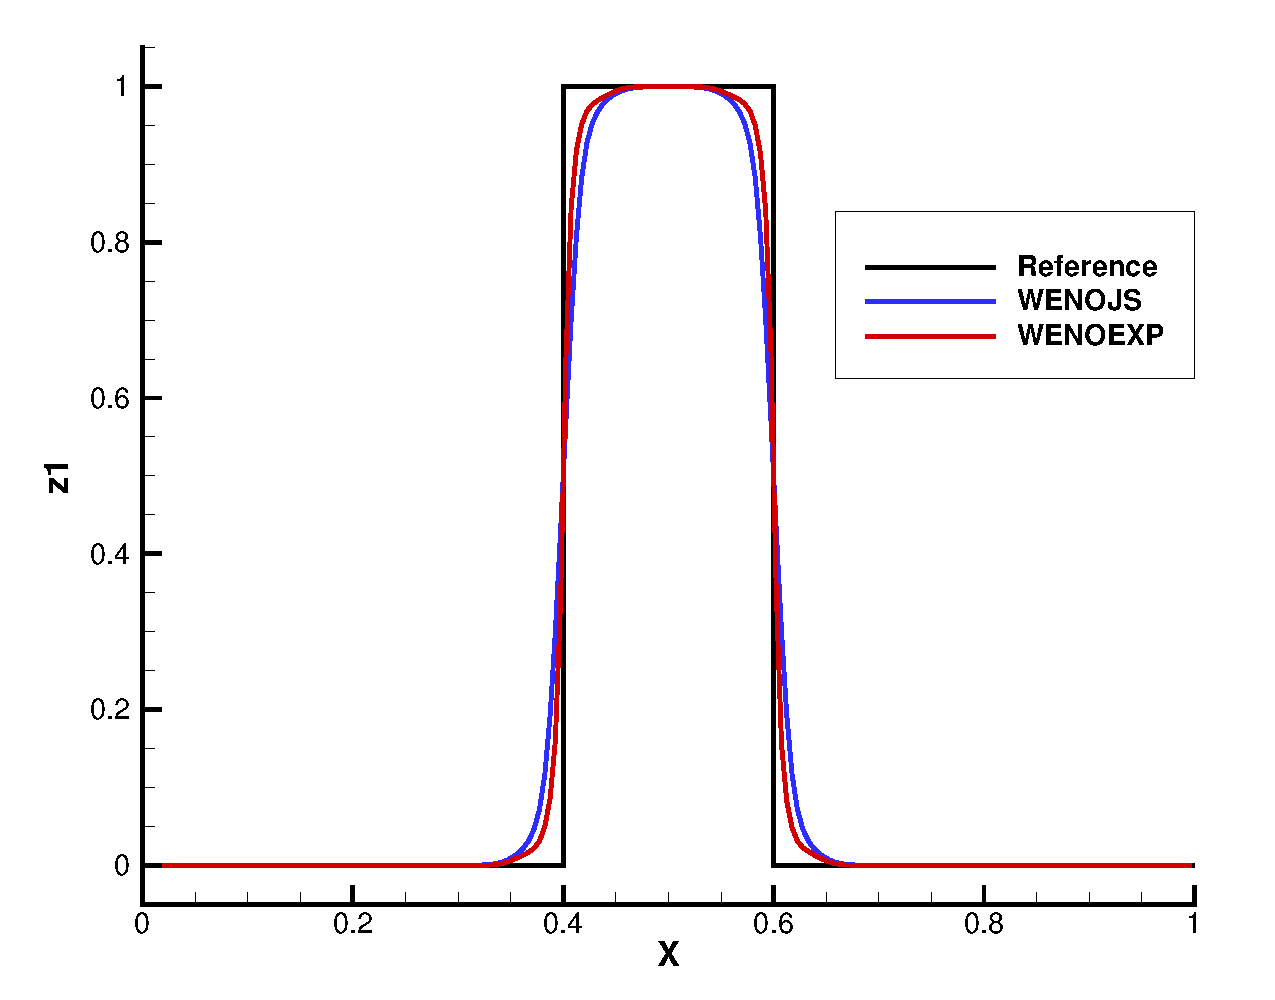
\includegraphics[width=\linewidth]{figure/1D-sharp/z1.eps}
        \caption{整体视图。}
    \end{subfigure}
    \hfill
    \begin{subfigure}[t]{0.45\linewidth}
        \centering
        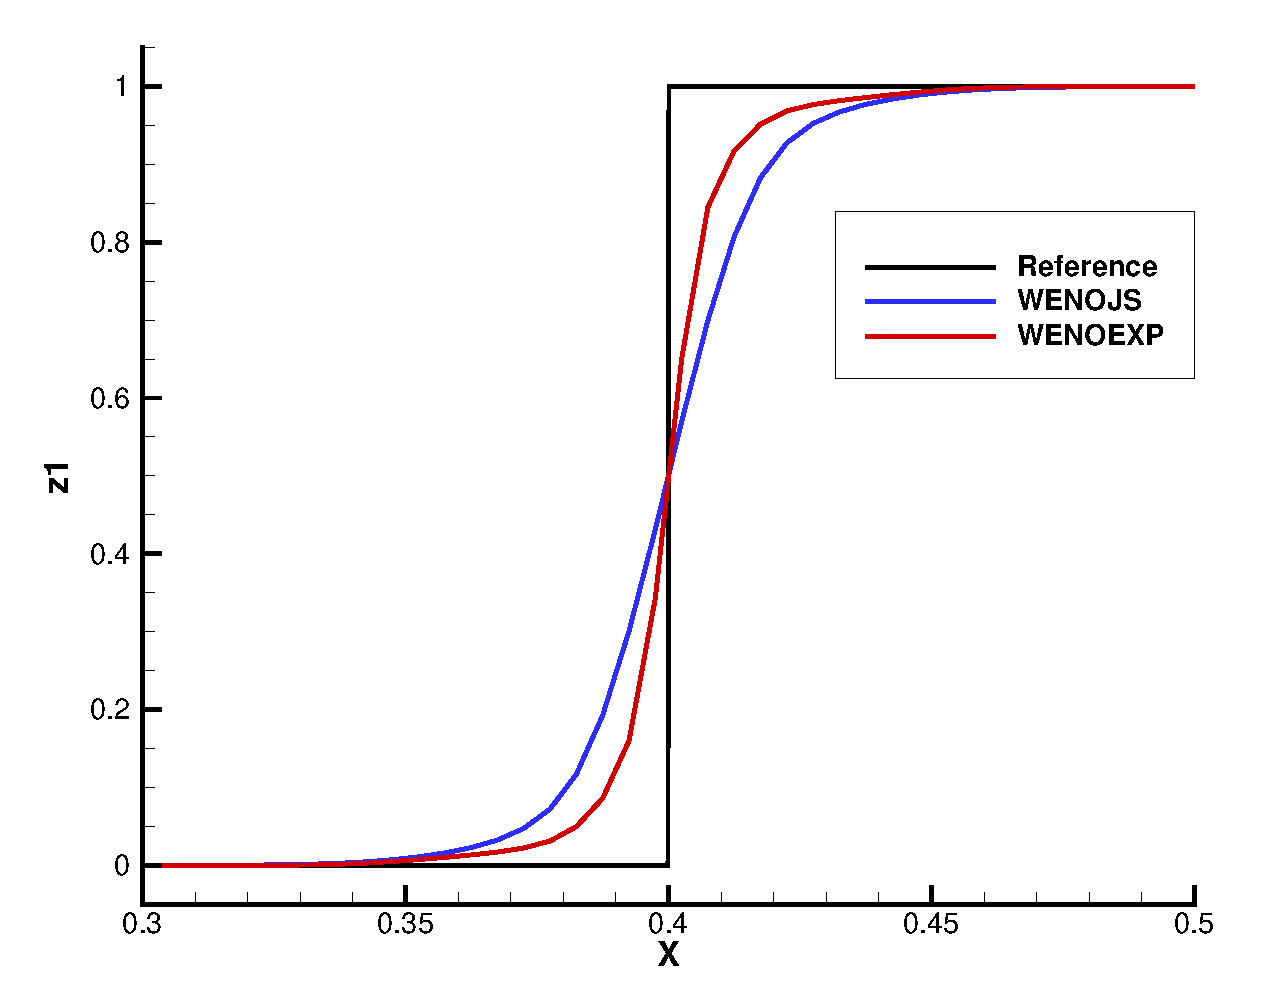
\includegraphics[width=\linewidth]{figure/1D-sharp/z1-large.eps}
        \caption{局部放大视图。}
    \end{subfigure}
    \caption{一维锐利界面平流问题中 WENO-JS 与 WENO-EXP 格式计算所得体积分数分布。}
    \label{fig:1D_sharp_z1}
\end{figure}

\autoref{fig:1D_sharp_oscillation} 展示了 WENO-EXP 格式在不同重构变量下的数值振荡情况。
结果表明，与采用守恒变量（conv）和原始变量一（prim1）重构的格式相比，
采用特征变量（char）和原始变量二（prim2）重构的格式所产生的振荡幅度显著更小，
改善幅度达 $5{\sim}7$ 个数量级。

\begin{figure}[!htbp]
    \centering
    \begin{subfigure}[t]{0.45\linewidth}
        \centering
        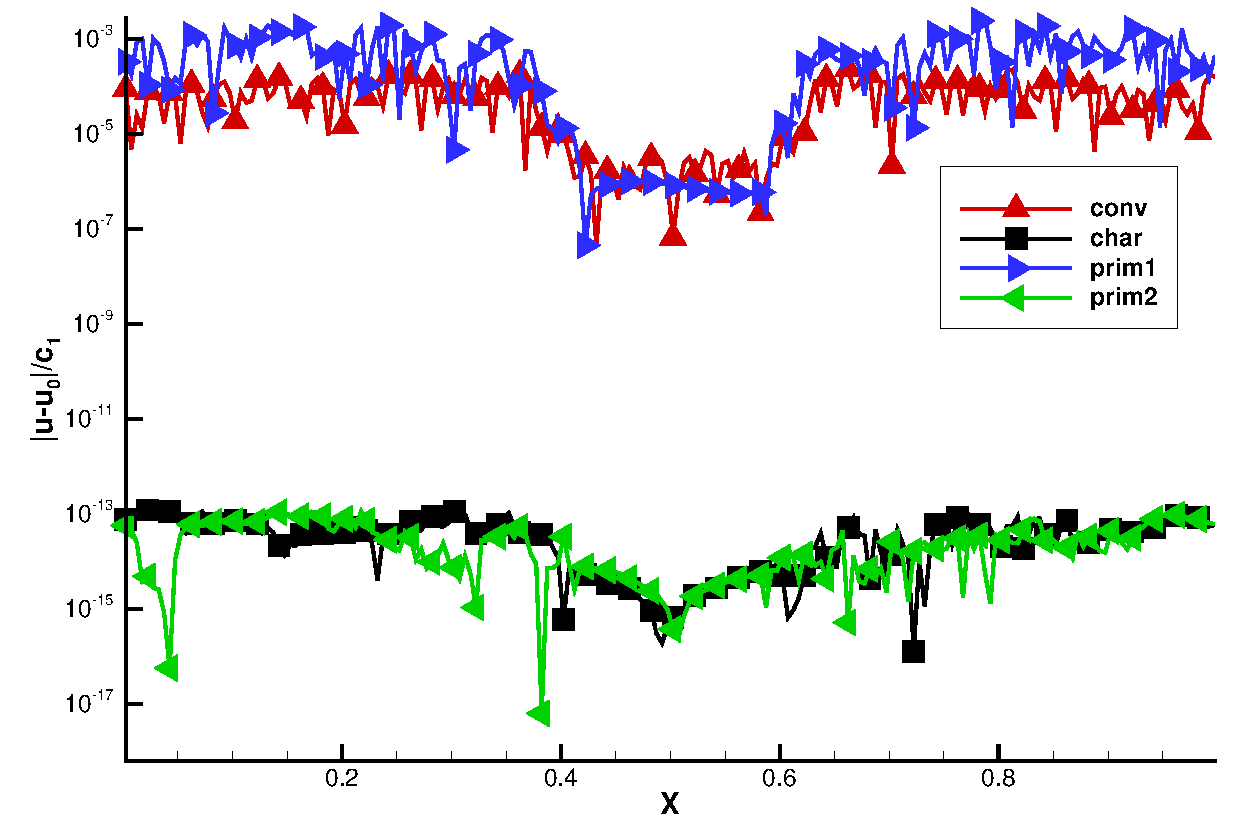
\includegraphics[width=\linewidth]{figure/1D-sharp/speed-eps-converted-to.pdf}
        \caption{速度振荡。}
    \end{subfigure}
    \hfill
    \begin{subfigure}[t]{0.45\linewidth}
        \centering
        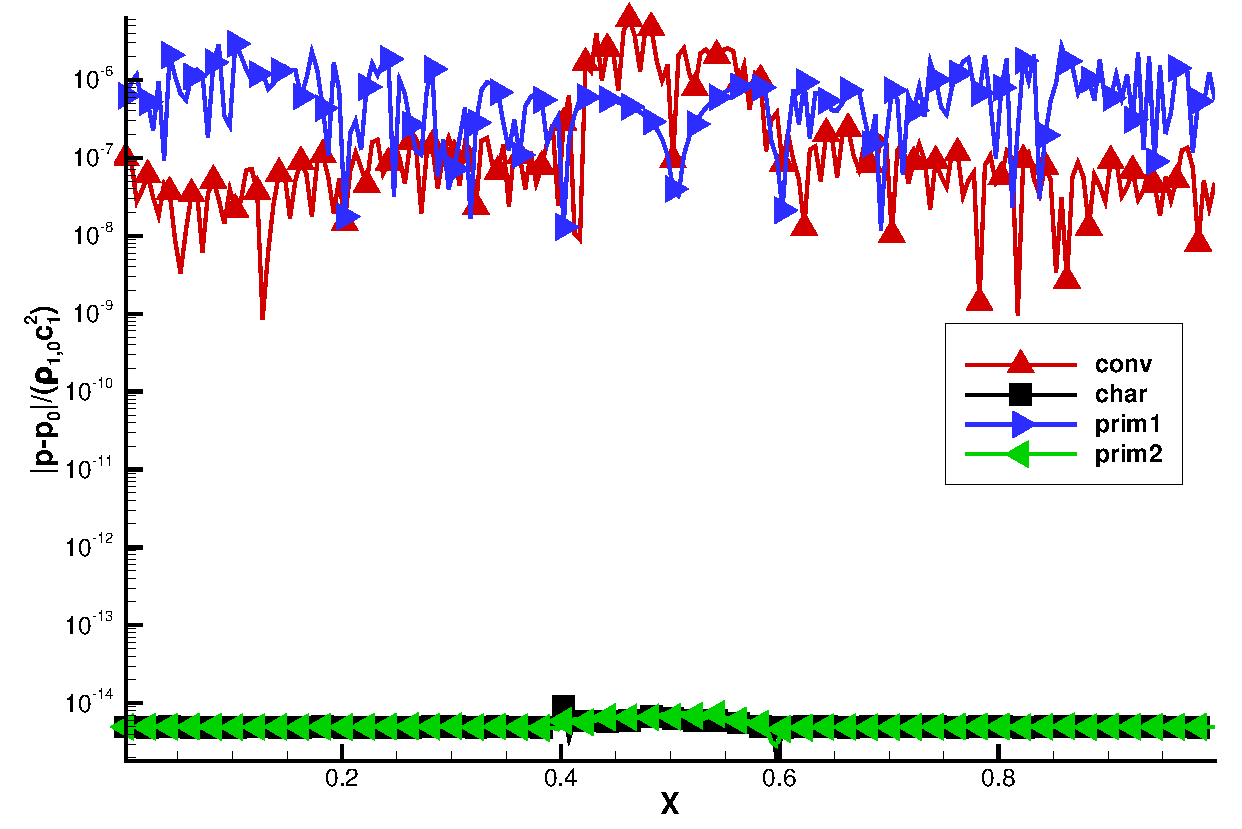
\includegraphics[width=\linewidth]{figure/1D-sharp/pre-eps-converted-to.pdf}
        \caption{压力振荡。}
    \end{subfigure}
    \caption{采用不同重构变量的 WENO-EXP 格式对一维锐利界面平流问题的数值振荡计算结果。}
    \label{fig:1D_sharp_oscillation}
\end{figure}


\subsection{二维光滑对流问题}

本算例将精度测试推广至二维情形。初始体积分数场设置为
\begin{equation}
    z_1(x, y, 0) = (0.5 - \varepsilon_z)\sin(2\pi(x + y)) + 0.5,
    \quad (x, y) \in [0, 1] \times [0, 1],
\end{equation}
其余参数与~\autoref{sec:1D_smooth_advection}节相同。

\autoref{tab:2d_smooth_compare} 列出了 WENO-JS 与 WENO-EXP 格式
在二维光滑对流问题中的数值误差与收敛阶数。
结果表明，WENO-JS 格式保持五阶收敛精度，
WENO-EXP 格式实现了六阶收敛精度，与一维情形的结论一致。

\begin{table}[!ht]
    \centering
    \caption{二维光滑对流问题体积分数 $z_1$ 的数值误差与收敛阶对比（$t = 1~\mathrm{s}$）。}
    \label{tab:2d_smooth_compare}
    \begin{tabular}{ccccccccc}
        \toprule
        & \multicolumn{4}{c}{WENO-JS} & \multicolumn{4}{c}{WENO-EXP} \\
        \cmidrule(lr){2-5} \cmidrule(lr){6-9}
        $N$
        & $L^\infty$ 误差 & 收敛阶
        & $L^1$ 误差 & 收敛阶
        & $L^\infty$ 误差 & 收敛阶
        & $L^1$ 误差 & 收敛阶 \\
        \midrule
        20  & 2.57E-03 & --   & 1.71E-03 & --   & 2.57E-03 & --   & 1.71E-03 & --   \\
        40  & 8.81E-05 & 4.87 & 4.96E-05 & 5.11 & 8.81E-05 & 4.87 & 4.96E-05 & 5.11 \\
        80  & 2.73E-06 & 5.01 & 1.47E-06 & 5.07 & 2.73E-06 & 5.01 & 1.47E-06 & 5.07 \\
        160 & 8.34E-08 & 5.03 & 4.46E-08 & 5.04 & 8.34E-08 & 5.03 & 4.46E-08 & 5.04 \\
        320 & 2.43E-09 & 5.10 & 1.37E-09 & 5.03 & 2.43E-09 & 5.10 & 1.37E-09 & 5.03 \\
        \bottomrule
    \end{tabular}
\end{table}


\subsection{二维锐利对流问题}
\label{sec:2D_sharp}

本算例考虑具有圆形锐利界面的二维对流问题，初始体积分数场设置为
\begin{equation}
    z_1(x, y, 0) = \begin{cases}
        1 - \varepsilon_z, & (x - 0.5)^2 + (y - 0.5)^2 < 0.1^2, \\
        \varepsilon_z,     & \text{其他},
    \end{cases}
\end{equation}
其余参数与一维锐利对流算例相同。
本算例用于评估所提格式在二维情形下的界面捕获能力和无振荡特性。

\autoref{fig:2Dinterface1} 给出了体积分数 $z_1$ 的整体分布及局部放大结果。
由图可见，所提格式能够清晰捕获圆形界面，且 WENO-EXP 格式所得界面厚度
相比 WENO-JS 格式更薄。

\begin{figure}[!htbp]
    \centering
    \subfloat[整体视图]{
        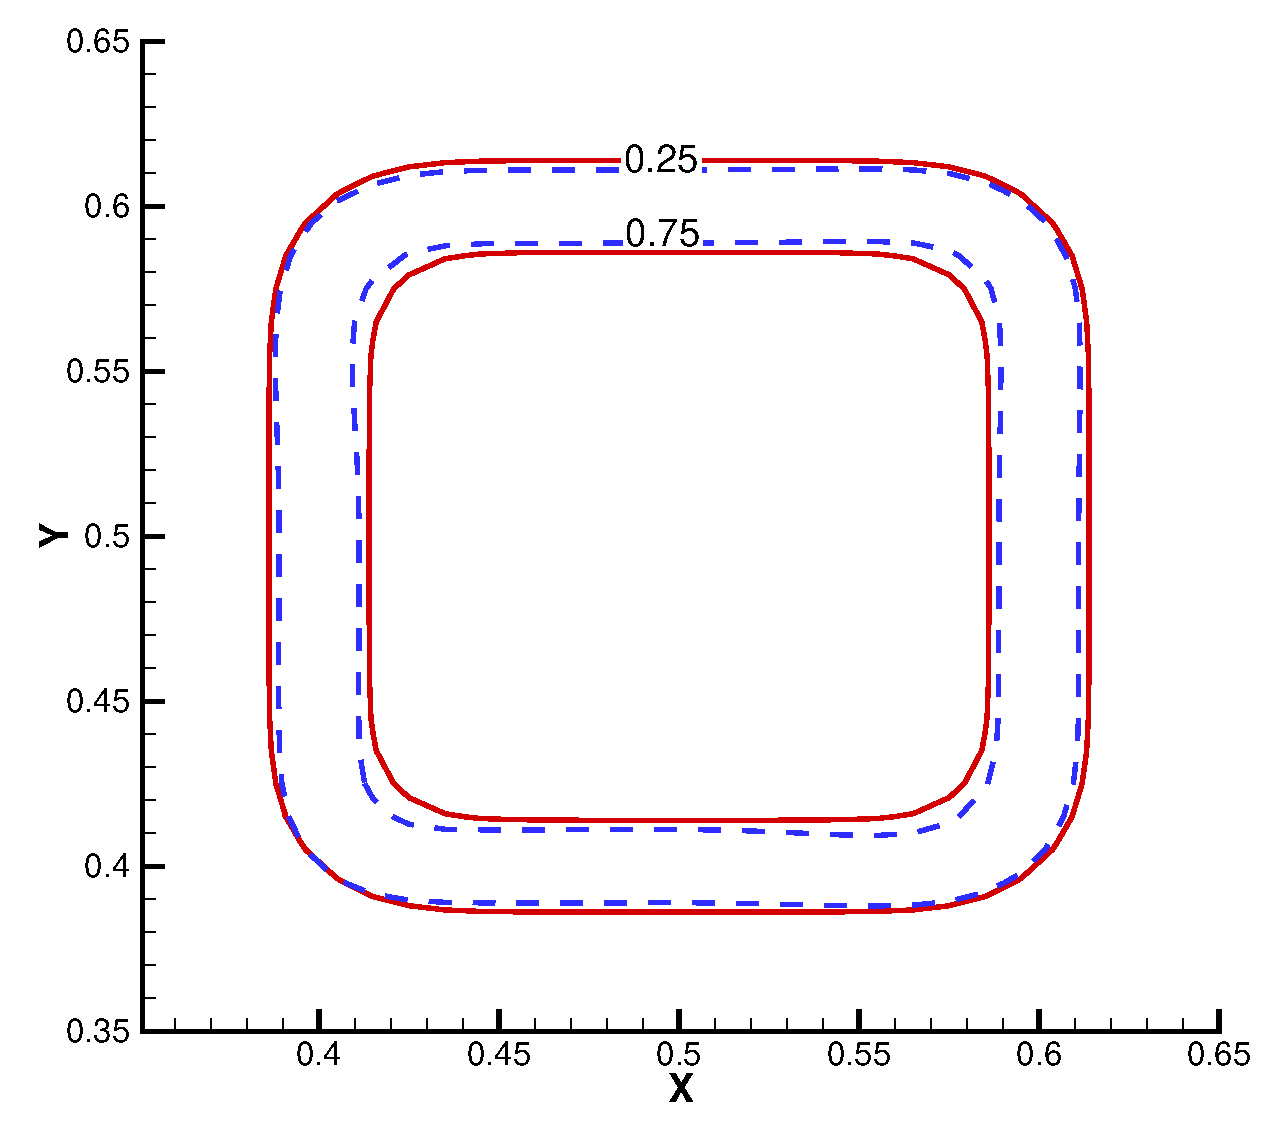
\includegraphics[width=0.45\textwidth]{figure/2D-sharp/large.eps}
    }
    \hfill
    \subfloat[局部放大视图]{
        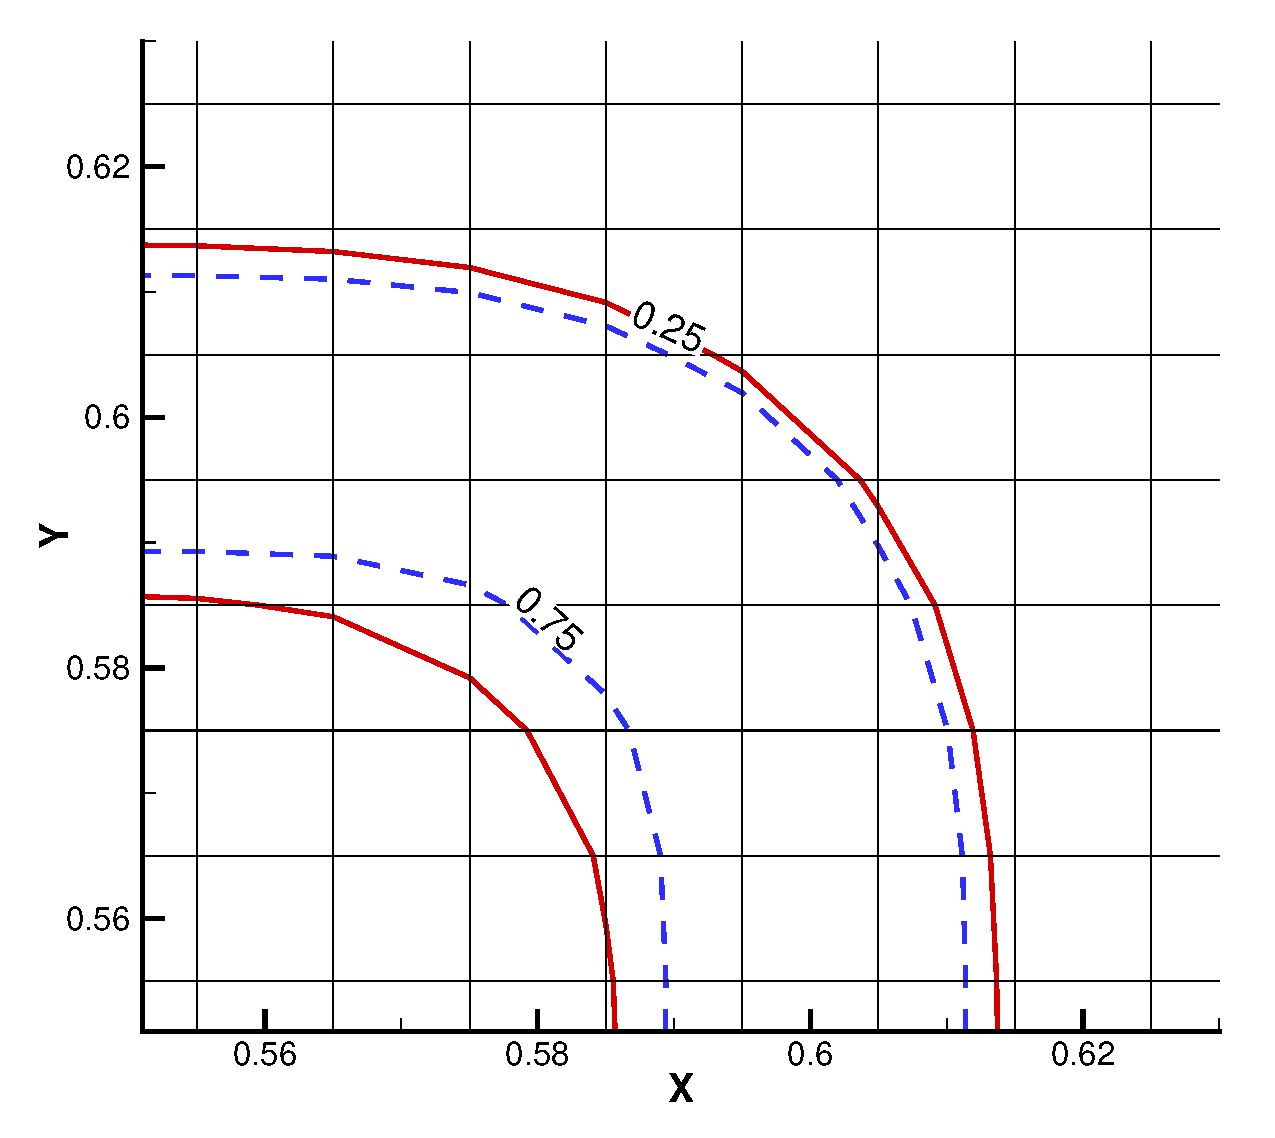
\includegraphics[width=0.45\textwidth]{figure/2D-sharp/small.eps}
    }
    \caption{二维锐利界面平流问题中体积分数分布
             （蓝色虚线：WENO-JS；红色实线：WENO-EXP）。}
    \label{fig:2Dinterface1}
\end{figure}

为定量刻画界面宽度，引入如下界面厚度指标：
\begin{equation}
    n_{\text{thickness}} = 1 \Big/ \max_{i,j}\Bigl(
        \bigl|\overline{(z_1)}_{i,j} - \overline{(z_1)}_{i+1,j}\bigr|,\;
        \bigl|\overline{(z_1)}_{i,j} - \overline{(z_1)}_{i,j+1}\bigr|
    \Bigr).
\end{equation}
$n_{\text{thickness}}$ 的值越小，对应的界面越锐利。
\autoref{fig:2Dinterface2} 展示了两种格式计算所得 $n_{\text{thickness}}$
的时间演化曲线。结果表明，WENO-EXP 格式所得 $n_{\text{thickness}}$
始终低于 WENO-JS 格式，且两者之间的差距随时间推移逐渐增大；
在 $t = 1~\mathrm{s}$ 时刻，WENO-EXP 格式的 $n_{\text{thickness}}$
较 WENO-JS 格式降低约 $25\%$。

\begin{figure}[!htbp]
    \centering
    \subfloat[$100\times 100$ 网格]{
        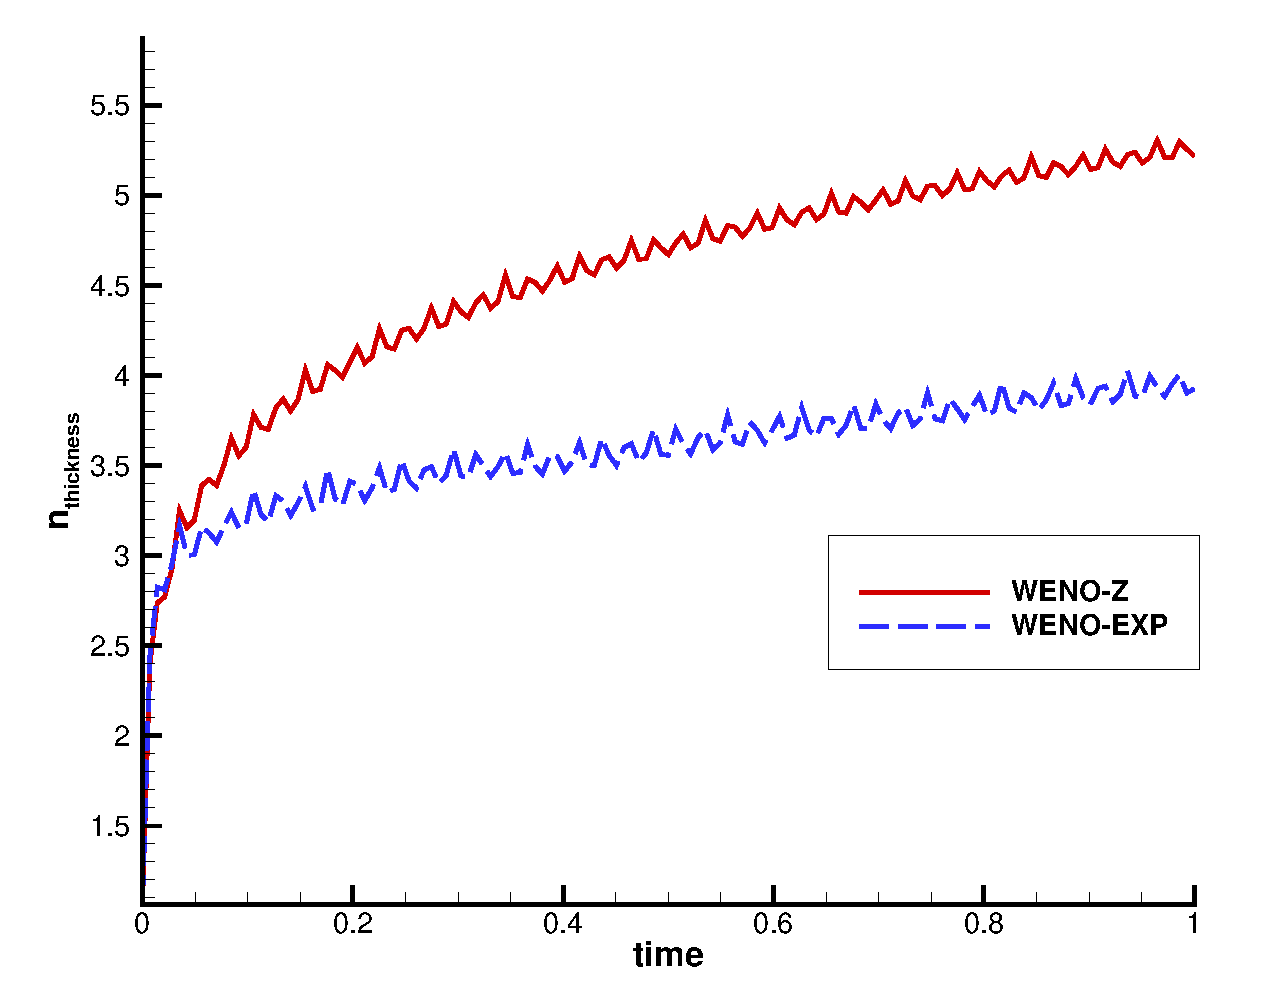
\includegraphics[width=0.45\textwidth]{figure/2D-sharp/100-thinckness.eps}
    }
    \hfill
    \subfloat[$200\times 200$ 网格]{
        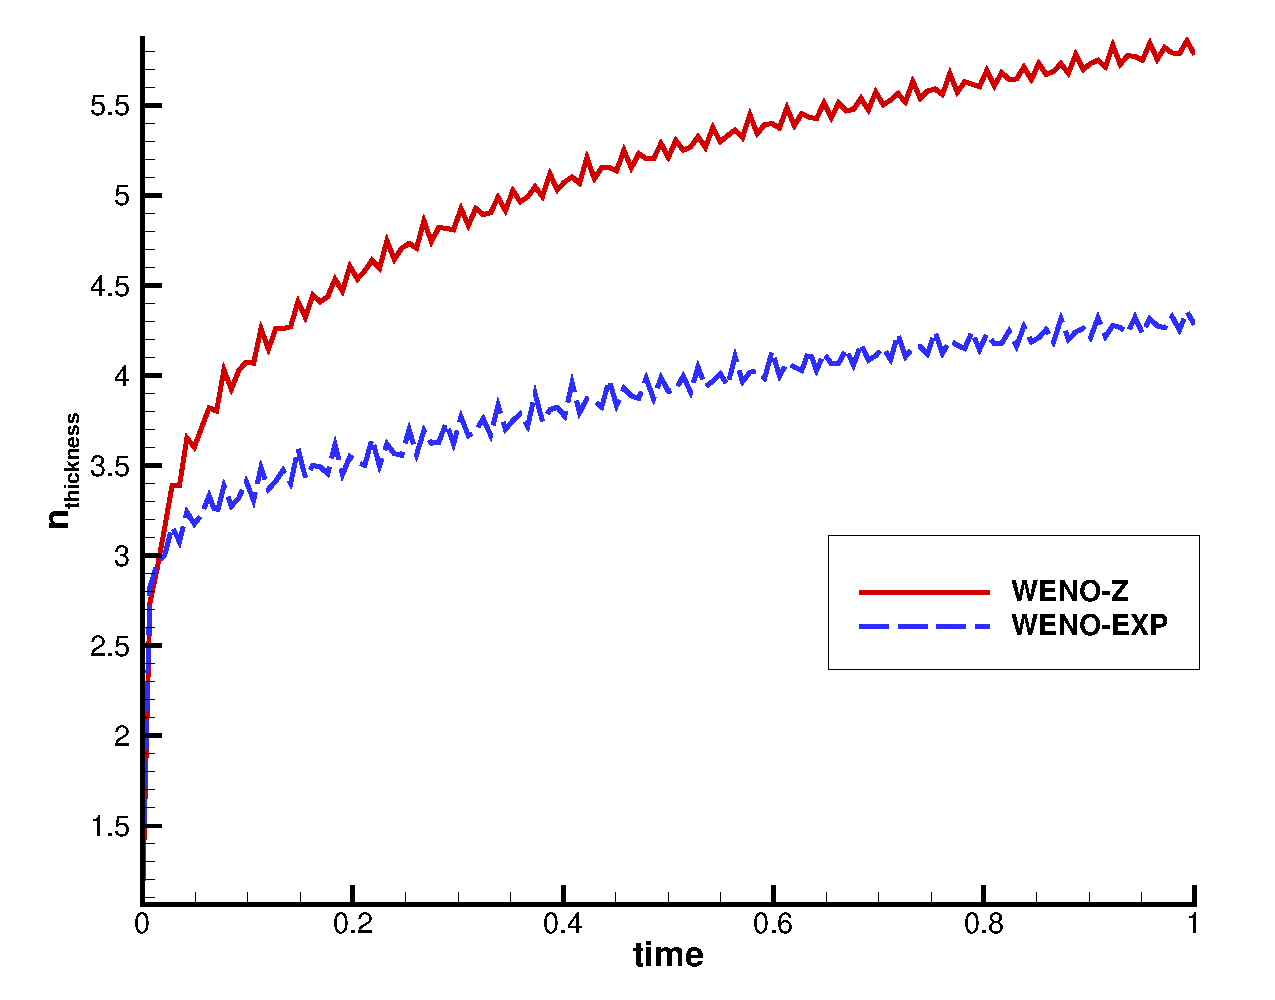
\includegraphics[width=0.45\textwidth]{figure/2D-sharp/200-thinckness.eps}
    }
    \caption{二维锐利界面平流问题界面厚度指标 $n_{\text{thickness}}$ 的时间演化。}
    \label{fig:2Dinterface2}
\end{figure}

\autoref{fig:2DOscillation} 展示了采用不同重构变量的 WENO-EXP 格式
所得速度与压力振荡情况。结果表明，基于 prim2 重构的 WENO-EXP 格式
在维持近似均匀压力场与速度场方面，相较于基于 prim1 重构的格式具有更优的性能，
该结论与一维算例所得结论一致。

\begin{figure}[!htbp]
    \centering
    \subfloat[速度振荡]{
        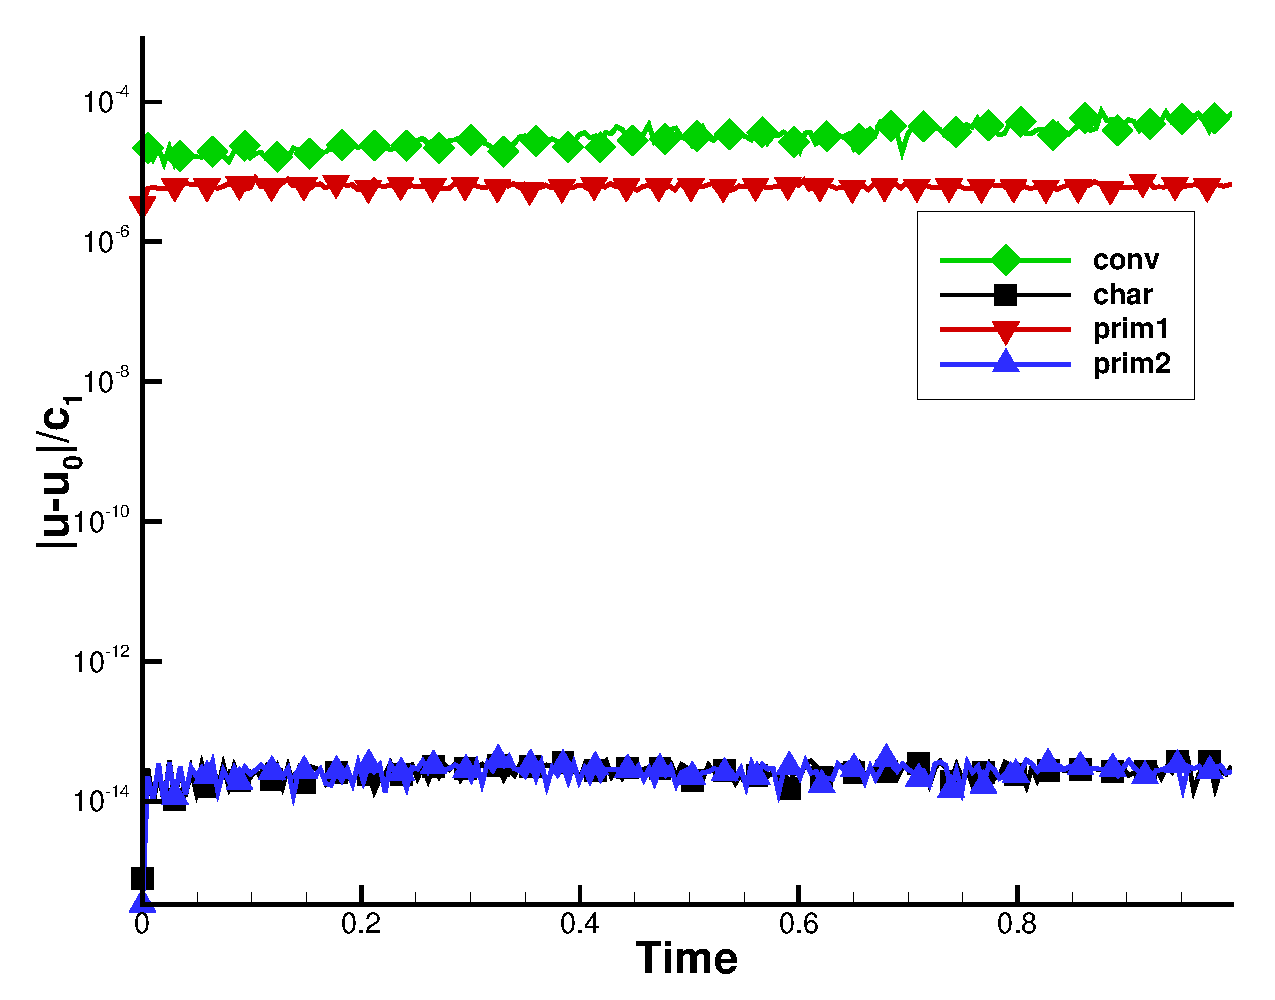
\includegraphics[width=0.45\textwidth]{figure/2D-sharp/speed.eps}
    }
    \hfill
    \subfloat[压力振荡]{
        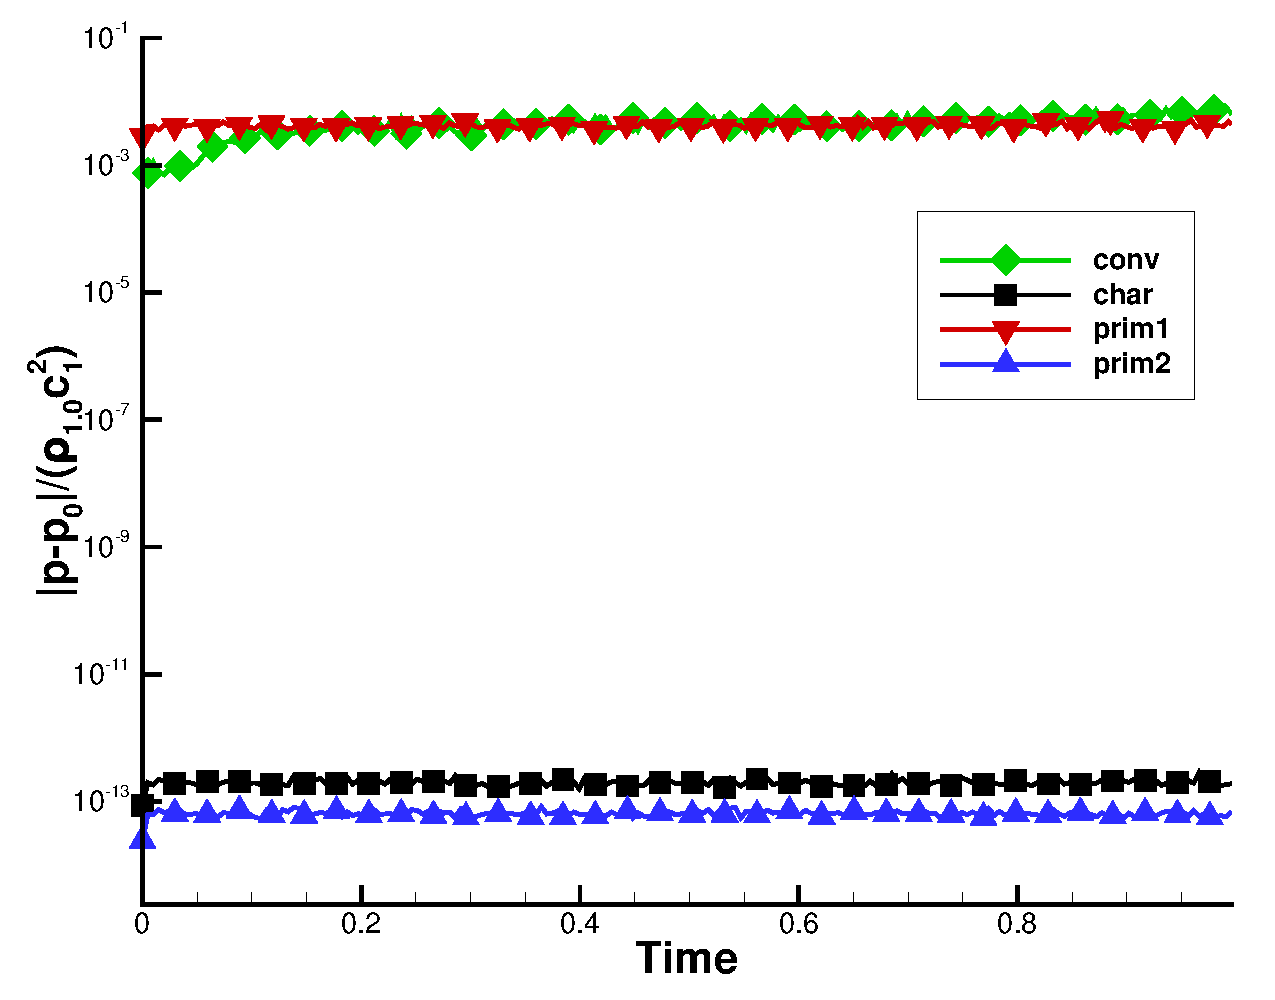
\includegraphics[width=0.45\textwidth]{figure/2D-sharp/pressure.eps}
    }
    \caption{采用不同重构变量的 WENO-EXP 格式对二维锐利界面平流问题的数值振荡计算结果。}
    \label{fig:2DOscillation}
\end{figure}

\autoref{tab:time_cost} 给出了采用不同重构变量的 WENO-EXP 格式的计算效率对比。
以守恒变量重构（conv）为基准，基于特征变量的重构格式（char）
由于引入了额外的特征分解过程，计算开销相应增加约 $30\%$；
而基于原始变量的两种重构格式（prim1 与 prim2）均保持了接近最优的计算效率。
上述结果表明，所提格式在保持高精度的同时，具有显著的计算效率优势。

\begin{table}[!htbp]
    \centering
    \caption{二维锐利界面对流问题的 CPU 计算时间。}
    \label{tab:time_cost}
    \begin{tabular}{lcccc}
        \toprule
        指标                & conv  & char  & prim1 & prim2 \\
        \midrule
        CPU 时间 (min)      & 35.81 & 46.34 & 37.56 & 36.93 \\
        相对计算开销        & 1.00  & 1.29  & 1.05  & 1.03  \\
        \bottomrule
    \end{tabular}
\end{table}


\subsection{低幅值驻波问题}

本算例考虑低幅值驻波问题~\cite{Sussman2007,Frandsen2003}，
用于验证所提格式在自由液面水动力学问题中的适用性。
初始时刻，空气与水在重力作用下静止于正方形容器
$\Omega = [0,\, 0.5~\mathrm{m}]^2$ 内，
容器四周为自由滑移固壁边界，初始构型如~\autoref{fig:low-amplitude-standing-wave} 所示。
\begin{figure}[!htbp]
    \centering
    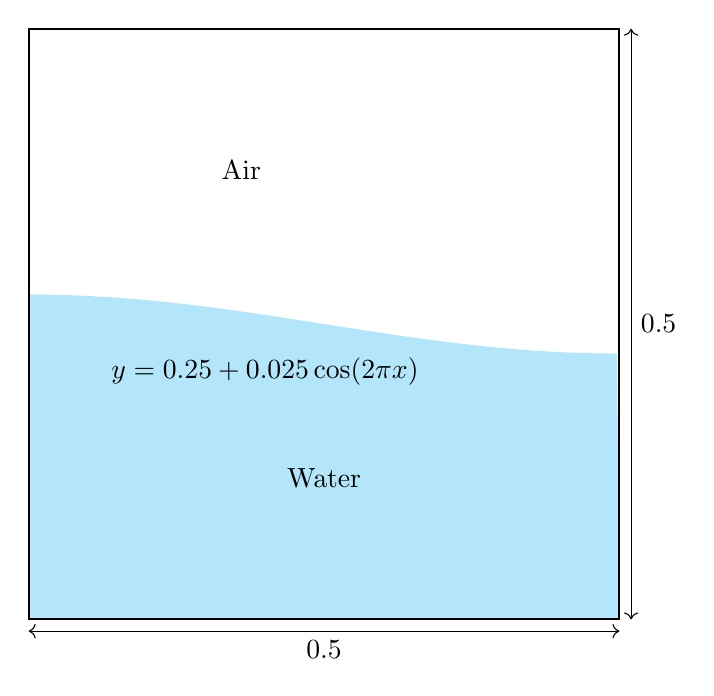
\begin{tikzpicture}[scale=15]


% Water region (blue fill, below interface)
\fill[cyan!30, domain=0:0.5, samples=200]
(0,0)
-- plot (\x, {0.25 + 0.025*cos(360*\x)})
-- (0.5,0)
-- cycle;

% Phase labels
\node at (0.18,0.38) {Air};
\node at (0.25,0.12) {Water};

% Gravity vector
% \draw[->, thick] (0.3,0.35) -- (0.3,0.25)
% node[midway, right] {$\boldsymbol{g}=(0,-2\pi)^{\mathrm{T}}$};

% ---- Dimension annotations ----
% Horizontal length 0.5
\draw[<->] (0,-0.01) -- (0.5,-0.01)
node[midway, below] {$0.5$};

% Vertical length 0.5
\draw[<->] (0.51,0) -- (0.51,0.5)
node[midway, right] {$0.5$};

% ---- Interface annotation ----
\node at (0.2,0.21)
{$y=0.25+0.025\cos(2\pi x)$};

% Domain boundary
\draw[thick] (0,0) rectangle (0.5,0.5);


\end{tikzpicture}

    \caption{低幅值驻波问题初始构型示意图。}
    \label{fig:low-amplitude-standing-wave}
\end{figure}

物理参数设置为：重力加速度 $\bm{g} = (0,\, -2\pi)^\top~\mathrm{m/s^2}$，
密度比 $\rho_{1,0}/\rho_{2,0} = 1000$，
两相声速均取 $c_1 = c_2 = 100~\mathrm{m/s}$，
背景压力 $p_0 = 10{,}000~\mathrm{Pa}$。水气界面可以用如下方程描述：
\begin{equation}
    \zeta(x,0) = h_s + A \cos(k_n x),
\end{equation}
其中，$h_s = 0.25~\mathrm{m}, A = 0.025~\mathrm{m}, k_n = 2\pi$. 偏离平衡位置的气-水界面在重力作用下产生周期性振荡，形成驻波。基于二阶小扰动理论~\cite{Frandsen2003}，液面 $\zeta(x, t)$ 的解析解可表示为如下级数展开式：
\begin{equation}
    \begin{aligned}
        \zeta(x, t)
        = &A\cos(\omega_n t)\cos(k_n x)\\
        &+ \frac{A^2\omega_n^2}{g}\cos(2k_n x)
          \Bigl(C_0 + C_1\cos(2\omega_n t) + C_2\cos(\omega_{2n} t)\Bigr)
        + \cdots,
    \end{aligned}
\end{equation}
其中
\begin{equation}
    \begin{aligned}
        C_0 &= \frac{1}{8}\frac{\omega_n^4 + g^2k_n^2}{\omega_n^4}, \\[6pt]
        C_1 &= \frac{1}{8}\frac{3\omega_n^4 - g^2k_n^2}{\omega_n^4}
               - \frac{3}{2}\frac{\omega_n^4 - g^2k_n^2}{\omega_n^2(4\omega_n^2 - \omega_{2n}^2)}, \\[6pt]
        C_2 &= \frac{1}{2}\frac{\omega_n^2\omega_{2n}^2 - \omega_n^4 - 3g^2k_n^2}
                              {\omega_n^2(4\omega_n^2 - \omega_{2n}^2)},\\[6pt]
        \omega_n &= \sqrt{g k_n \tanh(k_n h_s)},\\[6pt]
        \omega_{2n} &= \sqrt{g (2k_n) \tanh(2k_n h_s)};
    \end{aligned}
\end{equation}
其周期 $T$ 也有如下的近似表达式
\begin{equation}
    T = 2\pi / \sqrt{|g| k_n \tanh(k_n h_s)} \simeq 1.04~\mathrm{s}
\end{equation}

\autoref{fig:low-amplitude-standing-wave-exp} 展示了 WENO-JS 与 WENO-EXP 格式在 $128\times 128$ 网格下计算所得体积分数 $z_1$ 在 $t = 0.1~\mathrm{s}$与 $t = 1.0~\mathrm{s}$ 时刻的界面分布对比。由图可见，随着计算时间的推进，WENO-JS 格式在 $t = 1.0~\mathrm{s}$时刻出现了明显的界面弥散现象，界面厚度相比初始时刻显著增大；而 WENO-EXP 格式在相同时刻仍能保持较为锐利的界面轮廓，数值耗散明显低于 WENO-JS 格式，表明所提格式在大密度比自由液面长时间演化模拟中具有更强的界面捕捉能力。

\begin{figure}[!htbp]
    \centering
    \begin{subfigure}[t]{0.45\linewidth}
        \centering
        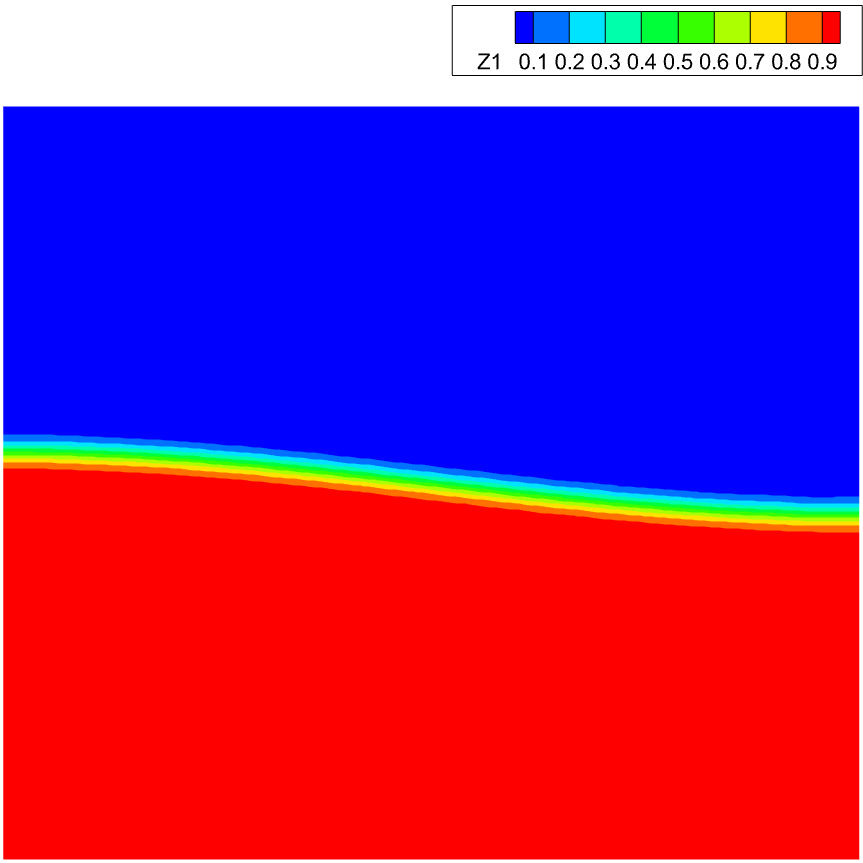
\includegraphics[width=\linewidth]{figure/problem-low-amplitude-standing-wave/z1/wenojs-1.png}
        \caption{WENO-JS 格式, $t=0.1$s。}
    \end{subfigure}
    \begin{subfigure}[t]{0.45\linewidth}
        \centering
        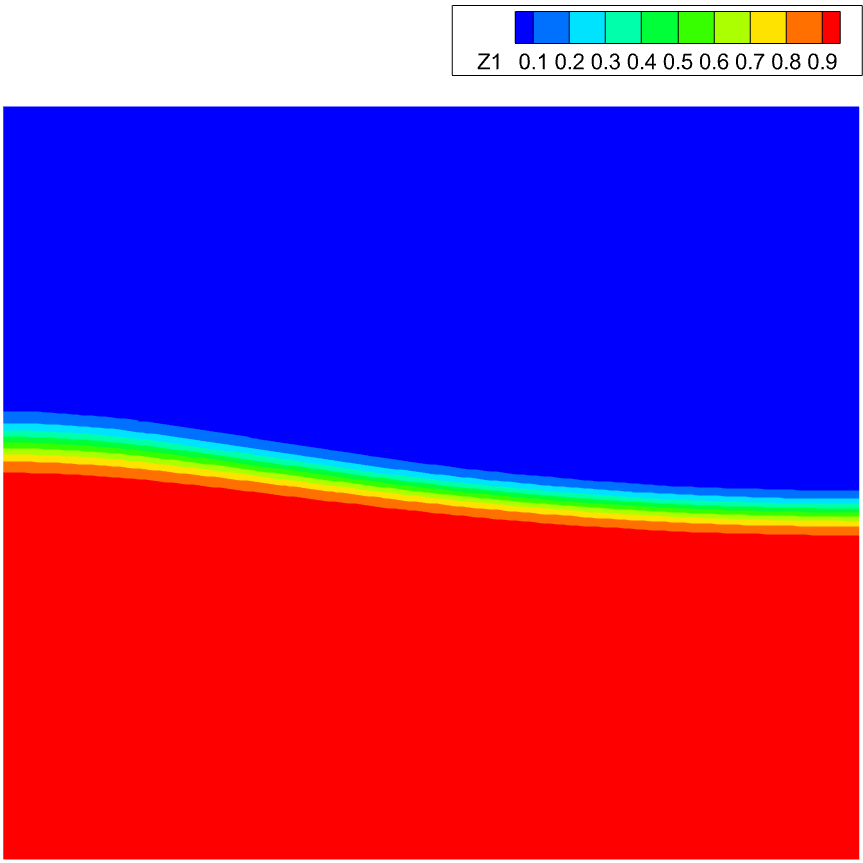
\includegraphics[width=\linewidth]{figure/problem-low-amplitude-standing-wave/z1/wenojs-10.png}
        \caption{WENO-JS 格式, $t=1.0$s。}
    \end{subfigure}
    \begin{subfigure}[t]{0.45\linewidth}
        \centering
        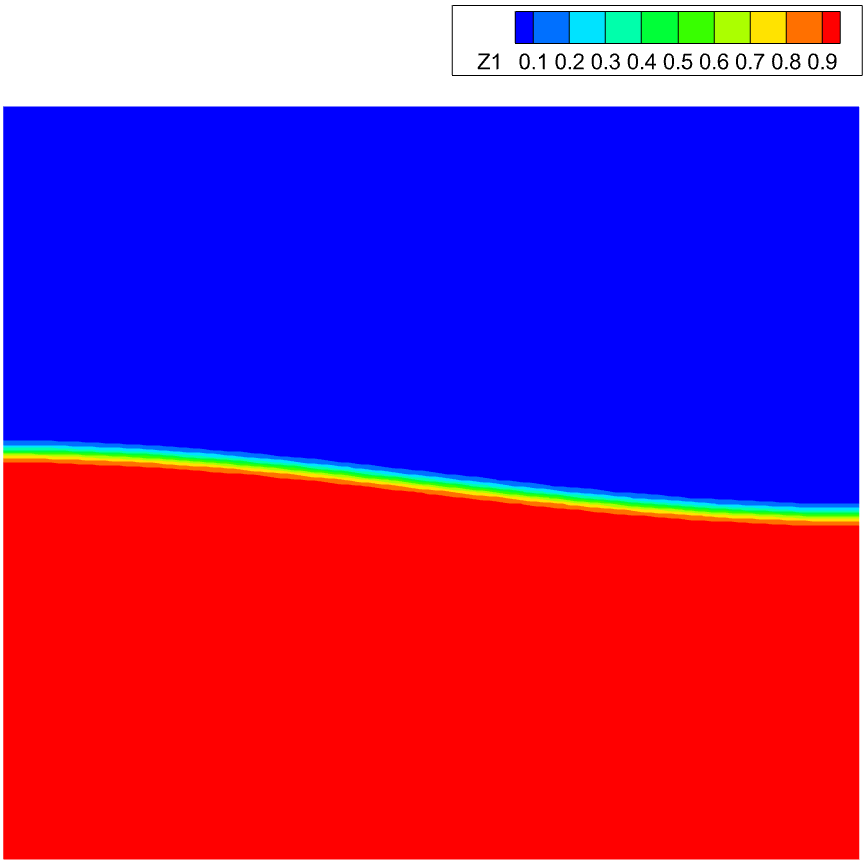
\includegraphics[width=\linewidth]{figure/problem-low-amplitude-standing-wave/z1/wenoexp-1.png}
        \caption{WENO-EXP 格式, $t=0.1$s。}
    \end{subfigure}
    \begin{subfigure}[t]{0.45\linewidth}
        \centering
        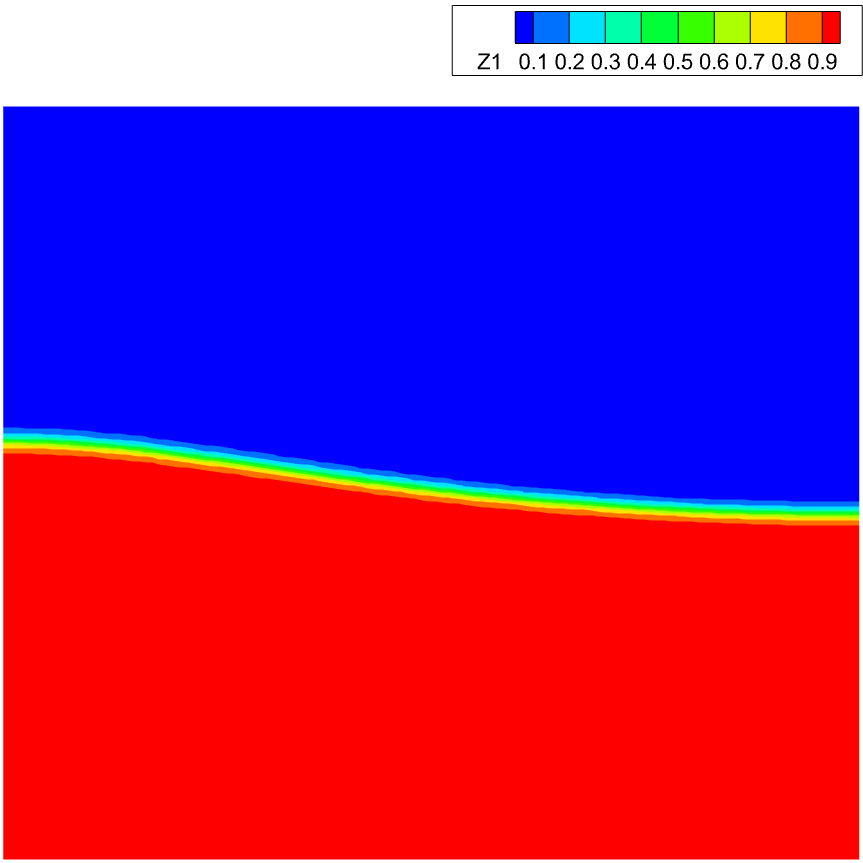
\includegraphics[width=\linewidth]{figure/problem-low-amplitude-standing-wave/z1/wenoexp-10.png}
        \caption{WENO-EXP 格式, $t=1.0$s。}
    \end{subfigure}
    \caption{体积分数 $z_1$ 随时间演化 $128\times 128$ 网格}
    \label{fig:low-amplitude-standing-wave-exp}
\end{figure}

\autoref{fig:low-amplitude-standing-wave-interface-history} 给出了左侧界面高度 $y_L(t)$ 与右侧界面高度 $y_R(t)$ 随时间的演化历程，并与参考解进行了对比。由图可见，WENO-JS 与 WENO-EXP 格式均能较好地捕捉气-水界面的周期性振荡特征，计算结果与参考解总体吻合良好。在长时间演化过程中，WENO-EXP 格式所得界面高度历程与参考解的吻合程度优于 WENO-JS 格式，幅值偏差均相对更小，表明所提格式在自由液面长时间动态模拟中具有更好的数值保真性。

\begin{figure}[!htbp]
    \centering
    \begin{subfigure}[t]{0.45\linewidth}
        \centering
        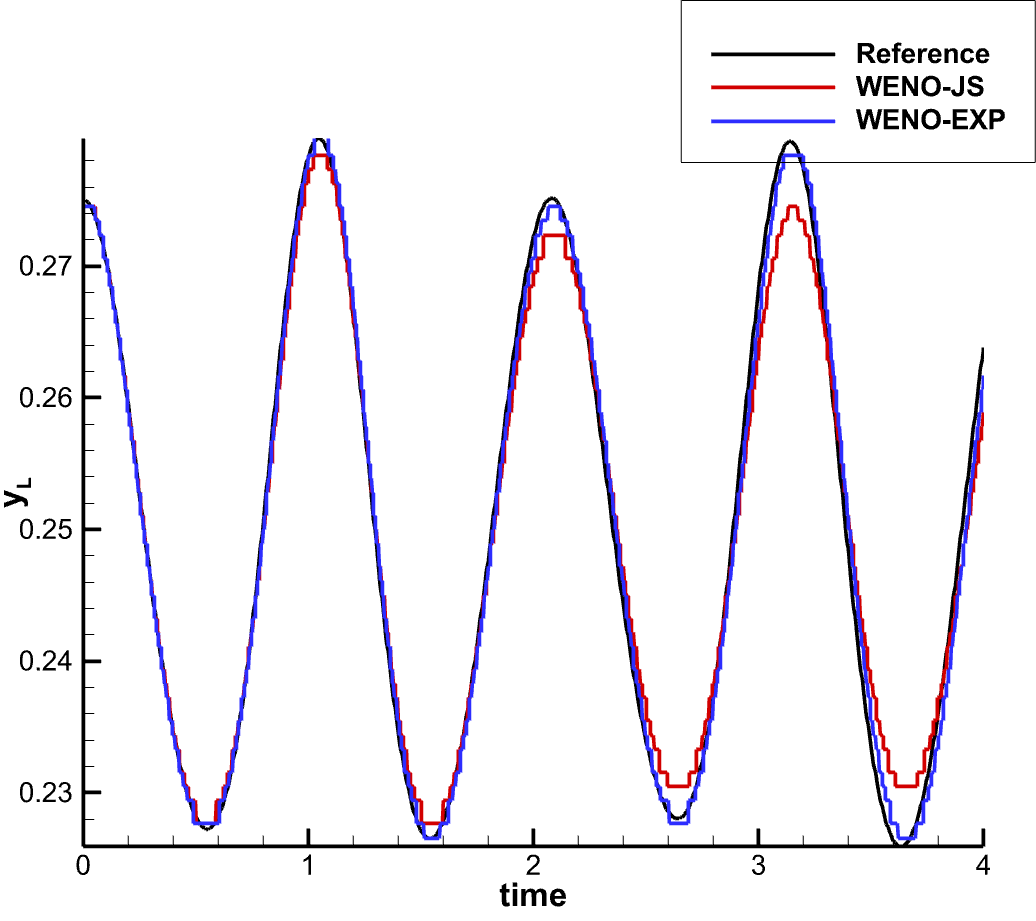
\includegraphics[width=\linewidth]{figure/problem-low-amplitude-standing-wave/interface/yL.png}
        \caption{$y_L(t)$}
    \end{subfigure}
    \hfill
    \begin{subfigure}[t]{0.45\linewidth}
        \centering
        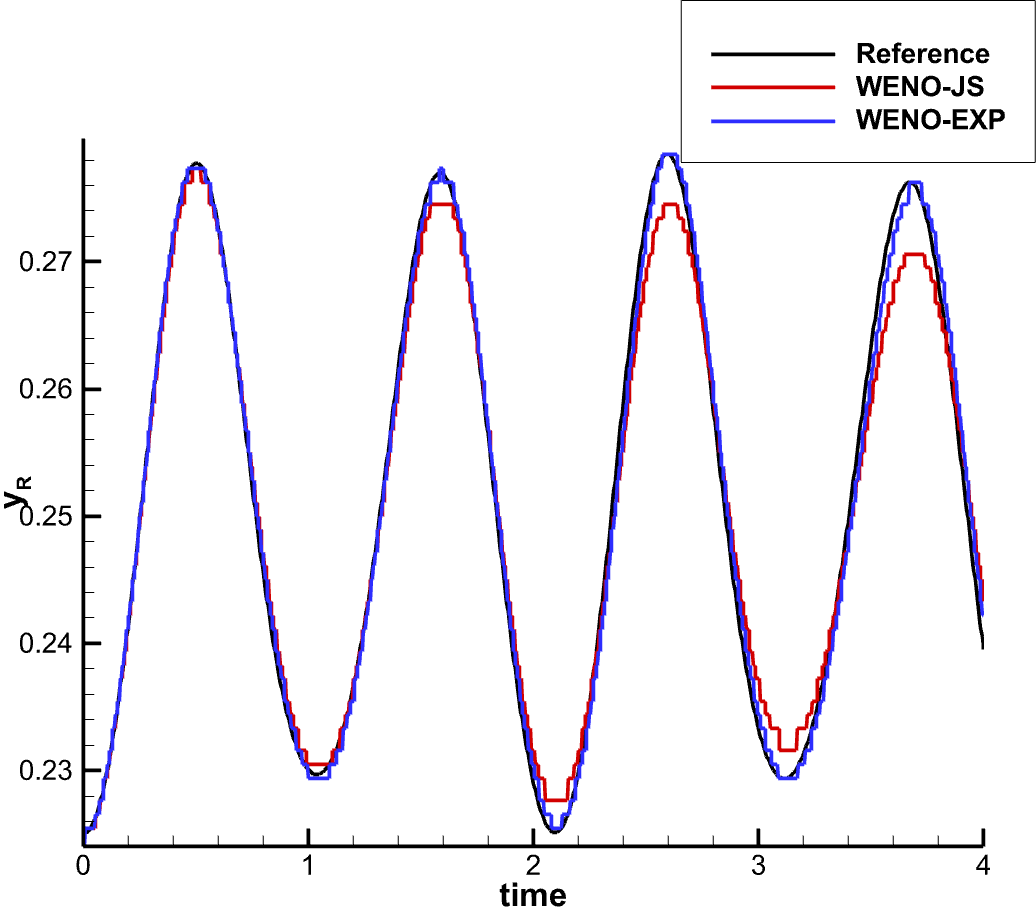
\includegraphics[width=\linewidth]{figure/problem-low-amplitude-standing-wave/interface/yR.png}
        \caption{$y_R(t)$}
    \end{subfigure}
    \caption{气-水界面高度随时间变化历程}
    \label{fig:low-amplitude-standing-wave-interface-history}
\end{figure}

\autoref{tab:low-amplitude-standing-wave-period} 列出了 WENO-JS 与 WENO-EXP 格式
在不同网格分辨率下数值计算所得的振荡周期。
结果表明，两种格式在各网格层次上均与理论值吻合良好，
且随网格加密，数值周期逐渐收敛至参考值。
WENO-EXP 格式与 WENO-JS 格式的计算结果相近，
表明所提格式在该问题中具有与经典格式相当的精度表现。

\begin{table}[!htbp]
    \centering
    \caption{低幅值驻波问题振荡周期（单位：s）。}
    \label{tab:low-amplitude-standing-wave-period}
    \begin{tabular}{lccc}
        \toprule
        网格 & $32 \times 32$ & $64 \times 64$ & $128 \times 128$ \\
        \midrule
        WENO-JS  & 1.00 & 1.03 & 1.05 \\
        WENO-EXP & 1.07 & 1.06 & 1.05 \\
        \bottomrule
    \end{tabular}
\end{table}

\subsection{线性晃荡问题}

\begin{figure}[!htbp]
    \centering
    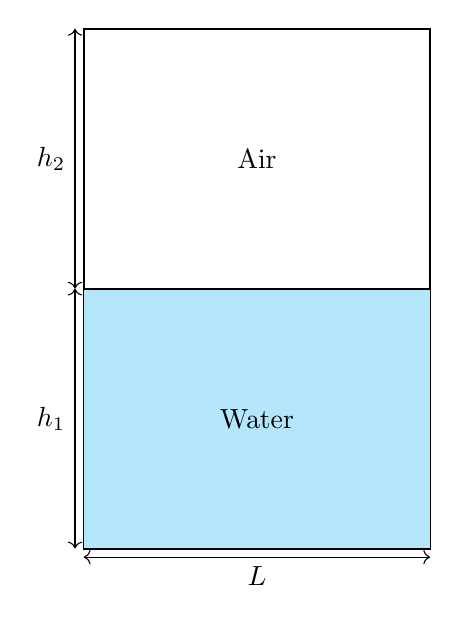
\begin{tikzpicture}[scale=1.1]

% Geometry parameters
\def\L{4}      % width
\def\Hone{3}   % water height h1
\def\Htwo{3}   % air height h2

% Outer boundary
\draw[thick] (0,0) rectangle (\L,\Hone+\Htwo);

% Water region (blue fill)
\fill[cyan!30] (0,0) rectangle (\L,\Hone);

% Interface
\draw[thick] (0,\Hone) -- (\L,\Hone);

% Phase labels
\node at (\L/2,\Hone+\Htwo/2) {Air};
\node at (\L/2,\Hone/2) {Water};


% Height h2
\draw[<->] (-0.1,\Hone) -- (-0.1,\Hone+\Htwo)
node[midway, left] {$h_2$};

% Height h1
\draw[<->] (-0.1,0) -- (-0.1,\Hone)
node[midway, left] {$h_1$};

% Width L
\draw[<->] (0,-0.1) -- (\L,-0.1)
node[midway, below] {$L$};

% % Acceleration a (horizontal)
% \draw[->] (\L+0.6,\Hone+1.2) -- (\L+1.6,\Hone+1.2)
% node[right] {$a$};

% % Gravity g (downward)
% \draw[->] (\L+1.1,\Hone+0.6) -- (\L+1.1,\Hone-0.6)
% node[midway, right] {$g$};

\end{tikzpicture}

    \caption{线性晃荡问题初始构型示意图。}
    \label{fig:linear-sloshing}
\end{figure}

本算例考虑二维线性晃荡问题~\cite{Chanteperdrix2004,grenier2013accurate}，
如~\autoref{fig:linear-sloshing} 所示。
初始时刻，空气与水在重力作用下于封闭水箱中保持静止，
水箱四周均为自由滑移固壁边界。当 $t > 0$ 时，
在整个流体域内沿 $x$ 轴正方向施加恒定水平加速度 $a$，
这等价于水箱以加速度 $-a\bm{e}_x$ 沿 $x$ 轴负方向突然起动的情形。
计算域为 $[0,\,1~\mathrm{m}] \times [0,\,2.25~\mathrm{m}]$，
初始水层高度 $h_1 = 1~\mathrm{m}$，初始气层高度 $h_2 = 1.25~\mathrm{m}$，
重力加速度 $g = 9.81~\mathrm{m/s^2}$，水平激励加速度 $a = 0.01g$，
两相声速均取 $c_1 = c_2 = 100~\mathrm{m/s}$。

基于线性化势流理论，界面高度 $\eta(x, t)$ 的解析解为~\cite{Chanteperdrix2004,grenier2013accurate}
\begin{equation}
    \eta(x, t) = \frac{a}{g}\left(
        x - \frac{L}{2}
        + \sum_{n=0}^{+\infty} \frac{4}{L\kappa_{2n+1}^2}
          \cos(\omega_{2n+1}t)\cos(\kappa_{2n+1}x)
    \right),
\end{equation}
其中
\begin{equation}
    \kappa_n = \frac{n\pi}{L},
    \qquad
    \omega_n = \sqrt{\frac{g\kappa_n(\rho_{1,0} - \rho_{2,0})}
                         {\rho_{1,0}\coth(\kappa_n h_1)
                          + \rho_{2,0}\coth(\kappa_n h_2)}}.
\end{equation}

\autoref{fig:linear-sloshing-history} 给出了水箱左、右壁处气-水界面高度
随时间变化的历程，分别基于三种均匀网格
（$64\times 144$、$128\times 288$ 及 $256\times 576$）计算得到。
\autoref{fig:linear-sloshing-interface} 给出了 $t = 1, 2, 3, 4~\mathrm{s}$
四个时刻通过 $z_1 = 0.5$ 等值线绘制的气-水界面形态。
数值结果与解析解之间的良好一致性表明，
所提格式能够准确模拟高密度比条件下含自由液面的线性晃荡流动。


\subsection{Rayleigh--Taylor 不稳定性问题}

\begin{figure}[!htbp]
    \centering
     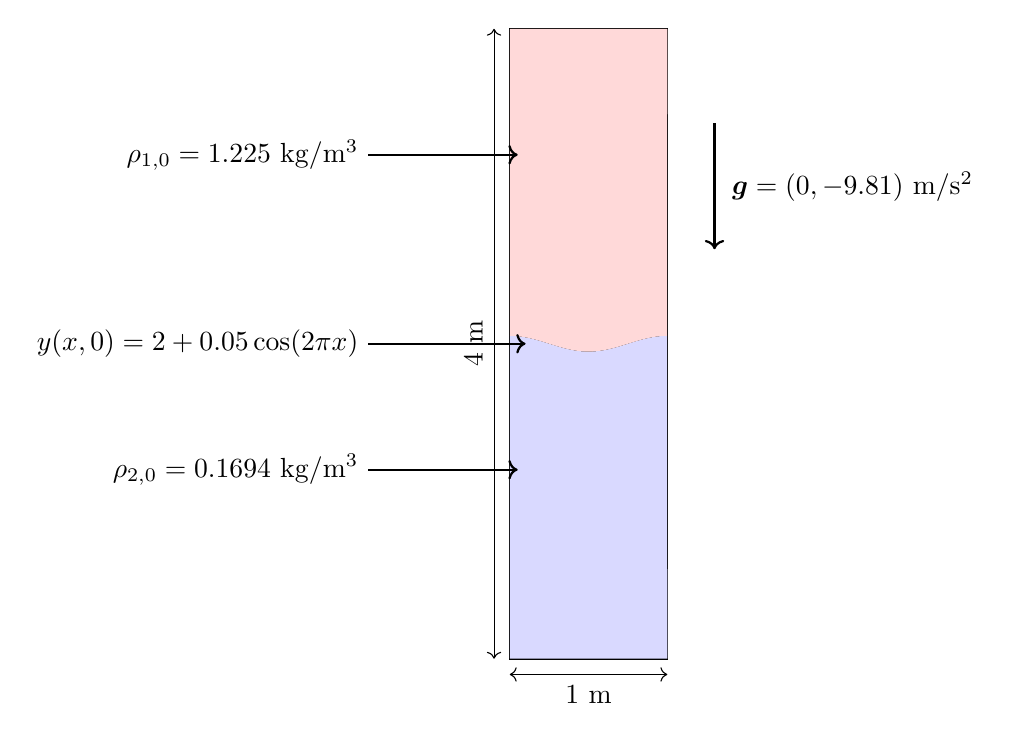
\begin{tikzpicture}[scale=2]

        %=====================
        % Domain
        %=====================
        \draw[thick] (0,0) rectangle (1,4);

        %=====================
        % Interface
        %=====================
        \draw[thick,domain=0:1,samples=200]
        plot (\x,{2 + 0.05*cos(2*pi*\x r)});

        %=====================
        % Fill regions
        %=====================
        \fill[blue!15,domain=0:1,samples=200]
        (0,0)
        -- plot (\x,{2 + 0.05*cos(2*pi*\x r)})
        -- (1,0) -- cycle;

        \fill[red!15,domain=0:1,samples=200]
        (0,4)
        -- plot (\x,{2 + 0.05*cos(2*pi*\x r)})
        -- (1,4) -- cycle;

        %=====================
        % Left-side annotations (densities & interface)
        %=====================

        % Upper fluid density
        \draw[->,thick] (-0.9,3.2) -- (0.05,3.2);
        \node[left,align=right] at (-0.9,3.2)
        {$\rho_{1,0}=1.225~\mathrm{kg/m^3}$};

        % Lower fluid density
        \draw[->,thick] (-0.9,1.2) -- (0.05,1.2);
        \node[left,align=right] at (-0.9,1.2)
        {$\rho_{2,0}=0.1694~\mathrm{kg/m^3}$};

        % Interface function
        \draw[->,thick] (-0.9,2.0) -- (0.1,2.0);
        \node[left,align=right] at (-0.9,2.0)
        {$y(x,0)=2+0.05\cos(2\pi x)$};

        %=====================
        % Gravity annotation (right side)
        %=====================
        \draw[->,thick] (1.3,3.4) -- (1.3,2.6);
        \node[right,align=left] at (1.35,3.0)
        {$\bm g=(0,-9.81)\ \mathrm{m/s^2}$};

        %=====================
        % Dimensions
        %=====================
        \draw[<->] (0,-0.1) -- (1,-0.1);
        \node at (0.5,-0.23) {$1~\mathrm{m}$};

        \draw[<->] (-0.1,0) -- (-0.1,4);
        \node[rotate=90] at (-0.23,2) {$4~\mathrm{m}$};

        %=====================
        % Boundary condition note
        %=====================
        % \node at (0.5,4.25) {Free-slip boundaries};

    \end{tikzpicture}
    \caption{Rayleigh--Taylor 不稳定性问题计算域及初始构型示意图。}
    \label{fig:RT_setup}
\end{figure}

本算例通过 Rayleigh--Taylor（RT）不稳定性问题~\cite{1997JCoPh.130..269P}
验证所提格式处理复杂界面流动的能力。
计算域为 $\Omega = [0,\,1~\mathrm{m}] \times [0,\,4~\mathrm{m}]$，
上层为重流体，密度 $\rho_{1,0} = 1.225~\mathrm{kg/m^3}$；
下层为轻流体，密度 $\rho_{2,0} = 0.1694~\mathrm{kg/m^3}$；
对应 Atwood 数
$\mathrm{At} = (\rho_{1,0} - \rho_{2,0})/(\rho_{1,0} + \rho_{2,0}) \approx 0.76$。
初始时刻流体静止，两相界面施加余弦扰动：
\begin{equation}
    y(x, 0) = 2 + 0.05\cos(2\pi x).
\end{equation}
重力加速度取 $\bm{g} = (0,\,-9.81~\mathrm{m/s^2})^\top$，
两相声速均设为 $c_1 = c_2 = 100~\mathrm{m/s}$，
背景压力 $p_0 = 10{,}000~\mathrm{Pa}$，
四周施加自由滑移边界条件，计算网格为 $64\times 256$。
问题构型如~\autoref{fig:RT_setup} 所示。

\autoref{fig:RTI-z1} 给出了采用本文方法在不同时刻的相界面演化云图。
结果表明，所提格式能够有效模拟界面扰动的复杂演化过程，
清晰捕获蘑菇状卷起结构及由 Kelvin--Helmholtz 二次不稳定所诱发的精细涡旋结构。

\autoref{fig:RTI-height} 进一步给出了相界面最高位置随时间的演化曲线，
并与文献~\cite{1997JCoPh.130..269P}中的参考结果进行对比，两者吻合良好，
验证了所提格式的准确性。
值得指出的是，在不启用保正限制器的情况下，
计算在相界面发生大变形阶段会因分相密度出现负值而中断，
直接说明了保正算法在高密度比复杂界面流动模拟中的必要性。


\subsection{溃坝流问题}

\begin{figure}[!htbp]
    \centering
    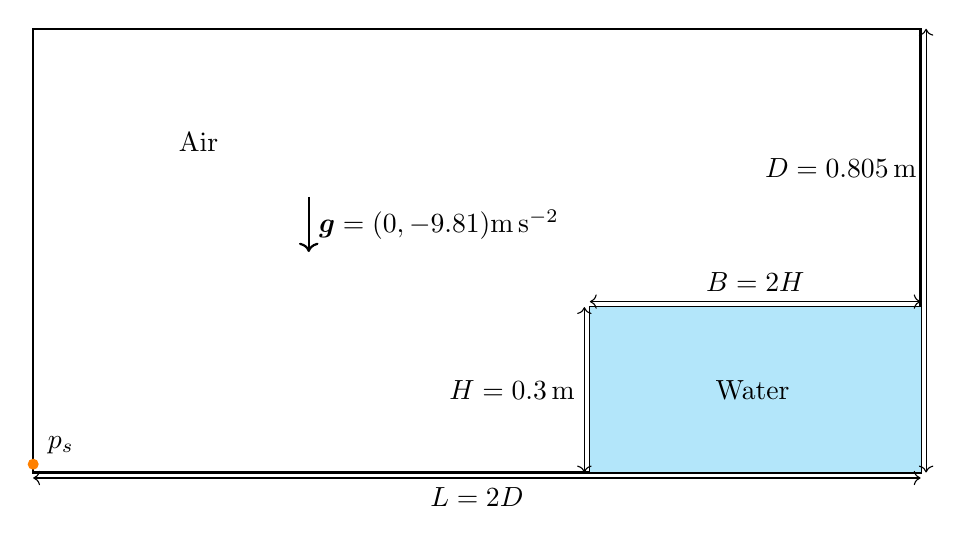
\begin{tikzpicture}[scale=0.7]
    % Draw the container
    \draw[thick] (0, 0) rectangle (16.1, 8.05);
    \draw[thick] (10.1, 0) rectangle (16.1, 3);

    % Fill the water with blue color
    \fill[cyan!30] (10.1, 0) rectangle (16.1, 3);


    % Add labels
    % \node[align=center] at (3, 6) {Air \\ $\rho_{2,0}=\SI{1.0}{\kilogram\per\cubic\meter}$};
    % \node[align=center] at (13.05, 1.5) {Water \\ $\rho_{1,0}=\SI{1000.0}{\kilogram\per\cubic\meter}$};

    % Add labels
    \node[align=center] at (3, 6) {Air};
    \node[align=center] at (13.05, 1.5) {Water};


    \node at (0.5, 0.5) {$p_s$};

    % gravity
    \draw[->, thick] (5,5) -- (5,4)
        node[midway, right] {$\bm{g} = (0, -9.81)\SI{}{\meter\per\second\squared}$};

    % Dimensions and arrows
    \draw[<->] (10.1, 3.1) -- (16.1, 3.1) node[midway, above] {$B = 2H$};
    \draw[<->] (16.2, 0) -- (16.2, 8.05) node[midway, left, yshift=30pt] {$D = \SI{0.805}{\meter}$};
    \draw[<->] (0, -0.1) -- (16.1, -0.1) node[midway, below] {$L = 2D$};
    \draw[<->] (10, 0) -- (10, 3) node[midway, left] {$H = \SI{0.3}{\meter}$};

    % Draw the point p_s
    \fill[orange] (0, 0.15) circle (0.1);

\end{tikzpicture}
    \caption{溃坝流问题的几何示意图。}
    \label{fig:dam-break}
\end{figure}

本算例考虑溃坝流问题，该问题已通过实验~\cite{LOBOVSKY2014407,Martin1952PartIA}
与数值方法~\cite{PARAMESWARAN2019405,Yang2020AHF}得到广泛研究，
用于评估所提格式在含剧烈相界面变形的弱可压缩两相流模拟中的鲁棒性与精度。

如~\autoref{fig:dam-break} 所示，初始时刻一个长 $B = 0.6~\mathrm{m}$、
高 $H = 0.3~\mathrm{m}$ 的矩形水柱在重力作用下保持静止，
重力加速度为 $\bm{g} = (0,\,-9.81~\mathrm{m/s^2})^\top$。
水柱置于充满空气的矩形容器
$\Omega = [0,\,1.61~\mathrm{m}] \times [0,\,0.805~\mathrm{m}]$ 中，
容器边界施加自由滑移边界条件。
压力传感器 $P_s$ 位于容器左壁，其中心距容器底部 $0.015~\mathrm{m}$。
计算网格取 $200\times 400$。

\autoref{fig:dambreak_interface} 给出了 WENO-JS 与 WENO-EXP 格式
在不同时刻的体积分数分布云图，
展示了水柱坍塌、水舌向前推进及与右壁碰撞后回溯的完整动态过程。
两种格式均成功完成了模拟，能够捕捉相界面的大变形特征；
其中，WENO-EXP 格式在相界面附近引入的数值耗散更小，
界面精细结构的保持更为完整。

\begin{figure}[!htbp]
    \centering
    \begin{subfigure}[t]{0.45\linewidth}
        \centering
        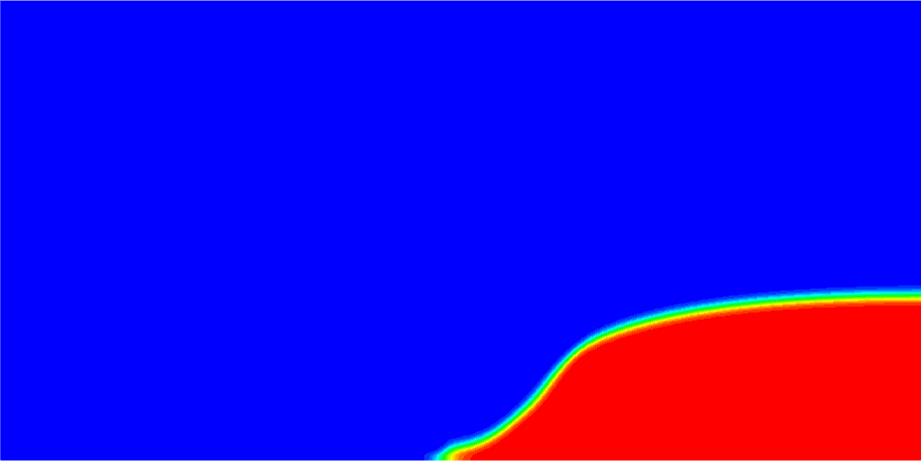
\includegraphics[width=\linewidth]{figure/dambreak/wenojs-1.png}
    \end{subfigure}
    \hfill
    \begin{subfigure}[t]{0.45\linewidth}
        \centering
        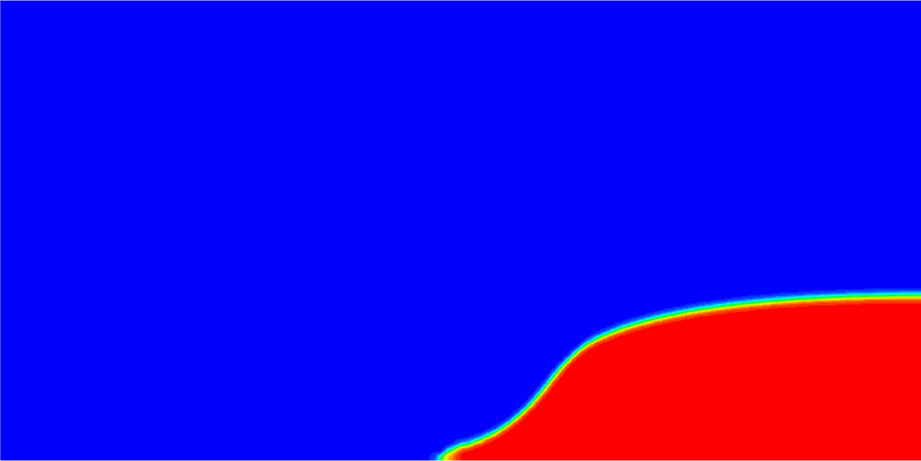
\includegraphics[width=\linewidth]{figure/dambreak/wenoexp1-1.png}
    \end{subfigure}\\
    \begin{subfigure}[t]{0.45\linewidth}
        \centering
        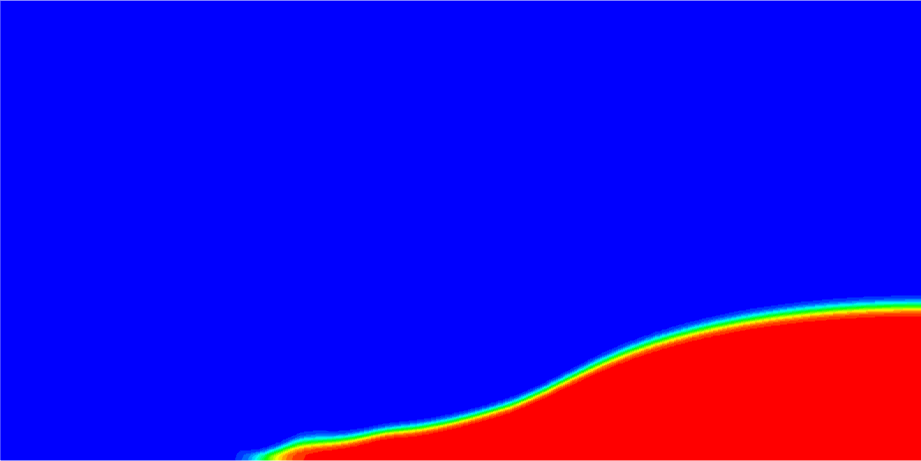
\includegraphics[width=\linewidth]{figure/dambreak/wenojs-2.png}
    \end{subfigure}
    \hfill
    \begin{subfigure}[t]{0.45\linewidth}
        \centering
        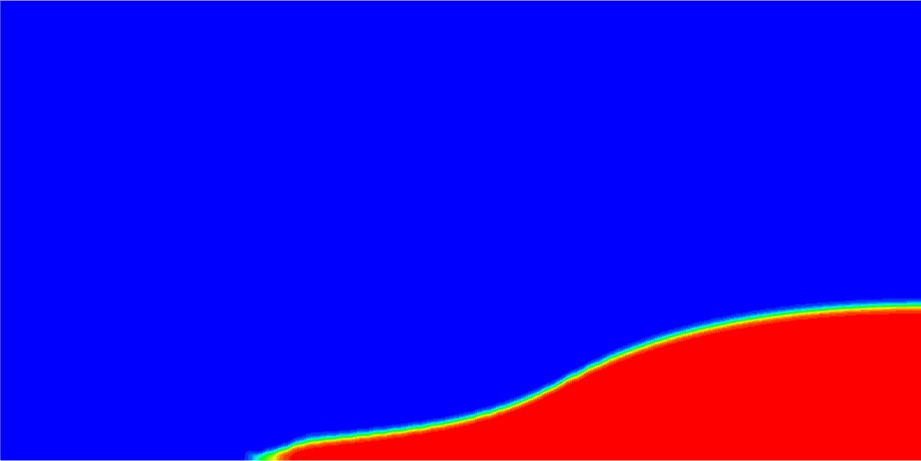
\includegraphics[width=\linewidth]{figure/dambreak/wenoexp1-2.png}
    \end{subfigure}\\
    \begin{subfigure}[t]{0.45\linewidth}
        \centering
        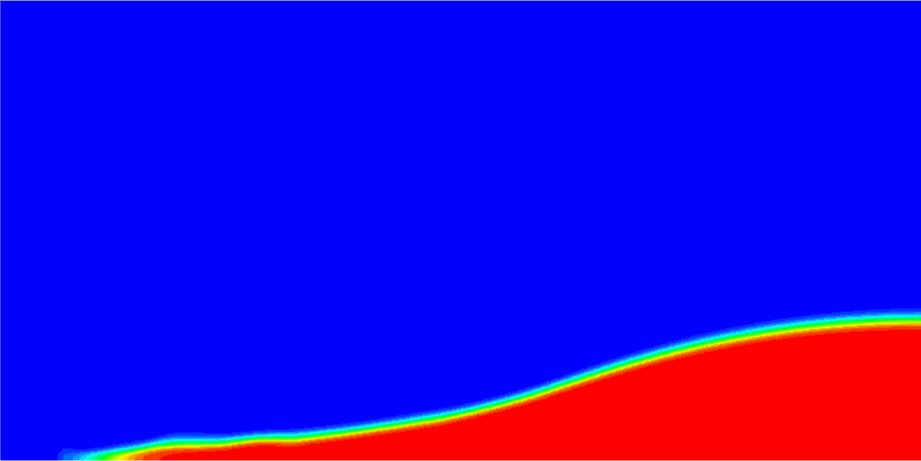
\includegraphics[width=\linewidth]{figure/dambreak/wenojs-3.png}
    \end{subfigure}
    \hfill
    \begin{subfigure}[t]{0.45\linewidth}
        \centering
        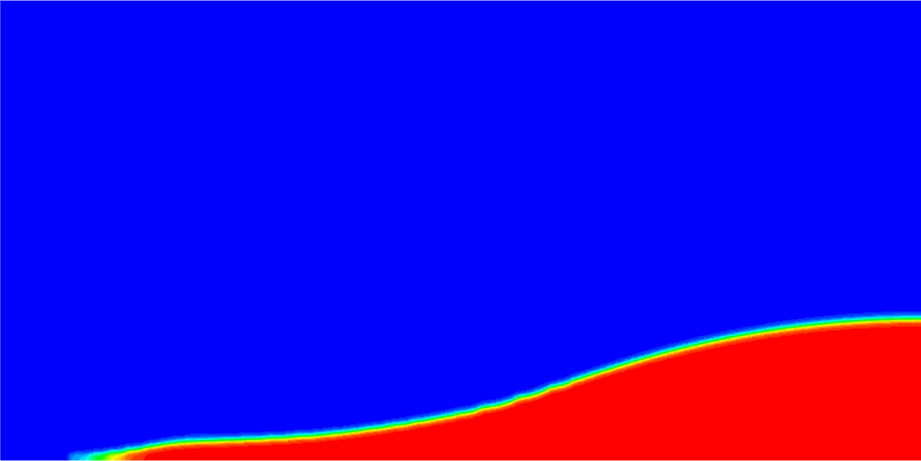
\includegraphics[width=\linewidth]{figure/dambreak/wenoexp1-3.png}
    \end{subfigure}\\
    \begin{subfigure}[t]{0.45\linewidth}
        \centering
        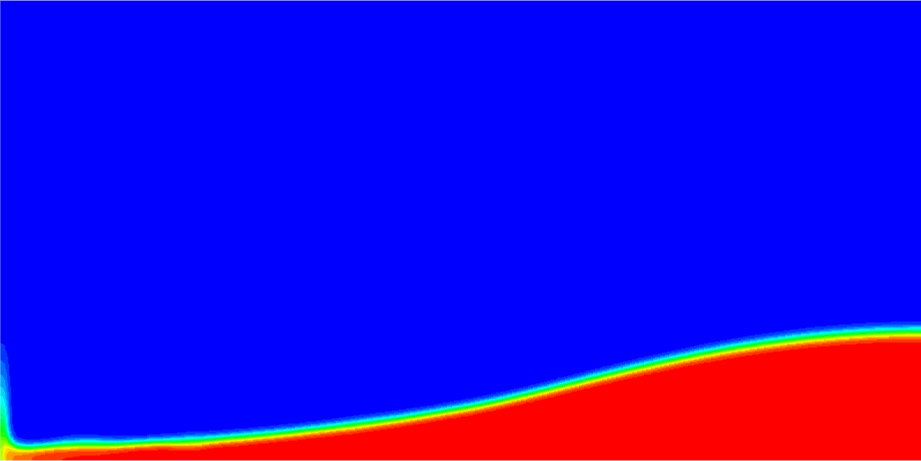
\includegraphics[width=\linewidth]{figure/dambreak/wenojs-4.png}
    \end{subfigure}
    \hfill
    \begin{subfigure}[t]{0.45\linewidth}
        \centering
        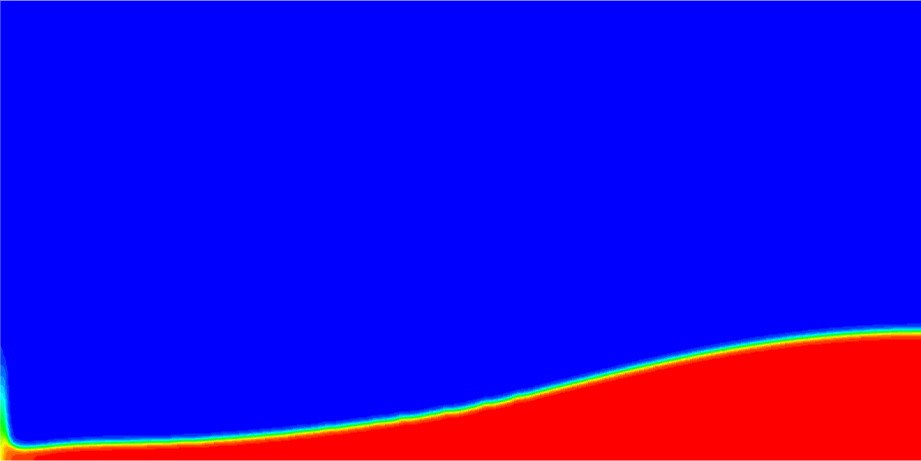
\includegraphics[width=\linewidth]{figure/dambreak/wenoexp1-4.png}
    \end{subfigure}\\
    \begin{subfigure}[t]{0.45\linewidth}
        \centering
        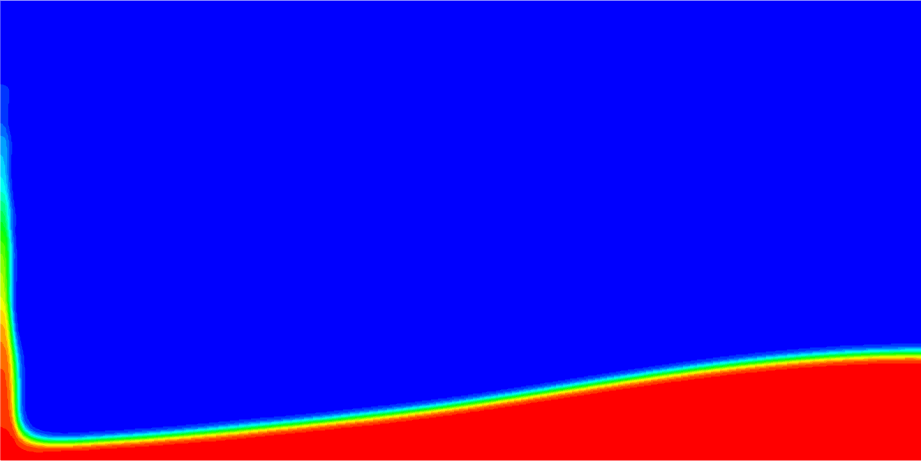
\includegraphics[width=\linewidth]{figure/dambreak/wenojs-5.png}
    \end{subfigure}
    \hfill
    \begin{subfigure}[t]{0.45\linewidth}
        \centering
        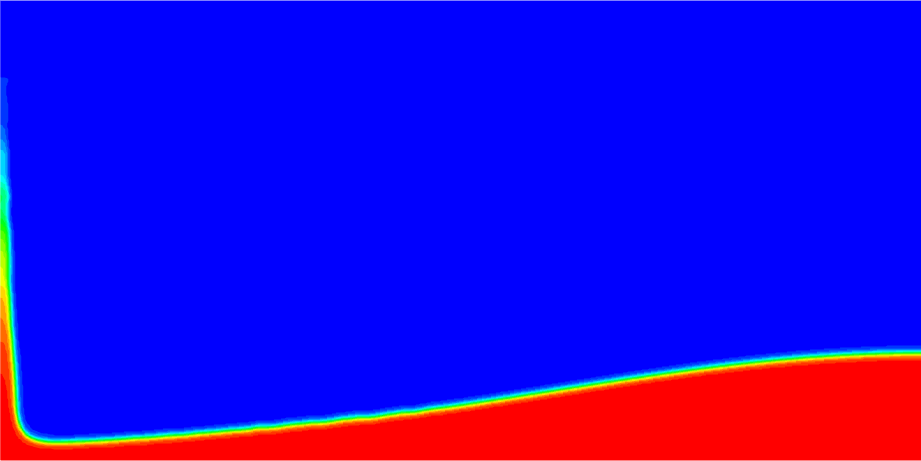
\includegraphics[width=\linewidth]{figure/dambreak/wenoexp1-5.png}
    \end{subfigure}\\
    \begin{subfigure}[t]{0.45\linewidth}
        \centering
        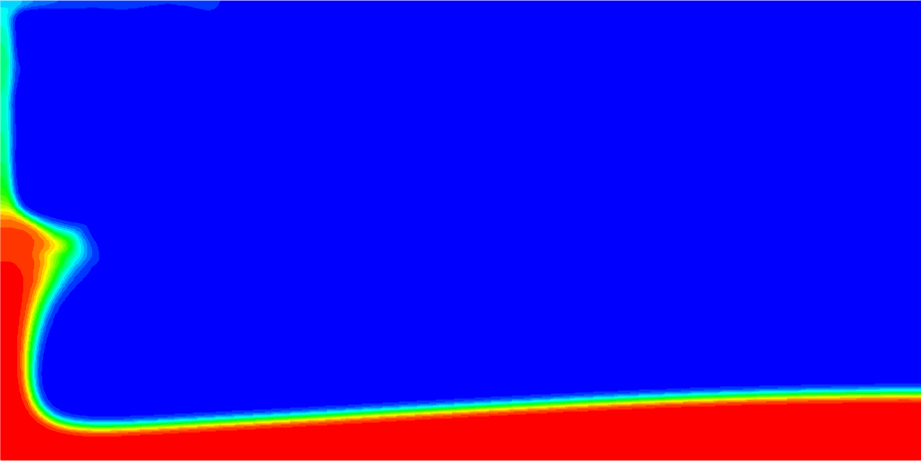
\includegraphics[width=\linewidth]{figure/dambreak/wenojs-6.png}
    \end{subfigure}
    \hfill
    \begin{subfigure}[t]{0.45\linewidth}
        \centering
        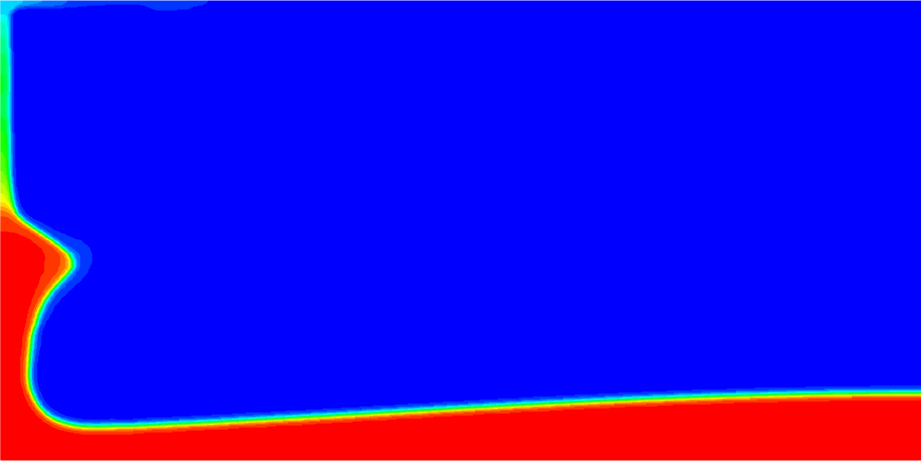
\includegraphics[width=\linewidth]{figure/dambreak/wenoexp1-6.png}
    \end{subfigure}\\
    \begin{subfigure}[t]{0.45\linewidth}
        \centering
        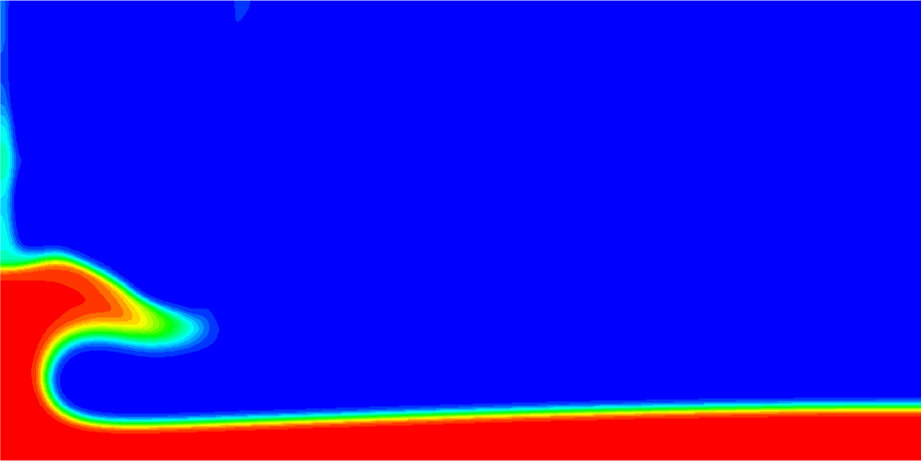
\includegraphics[width=\linewidth]{figure/dambreak/wenojs-7.png}
    \end{subfigure}
    \hfill
    \begin{subfigure}[t]{0.45\linewidth}
        \centering
        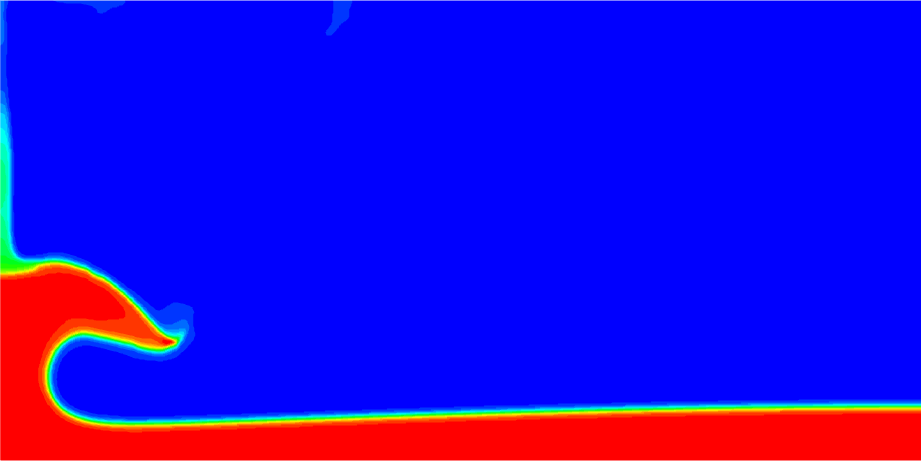
\includegraphics[width=\linewidth]{figure/dambreak/wenoexp1-7.png}
    \end{subfigure}\\
    \begin{subfigure}[t]{0.45\linewidth}
        \centering
        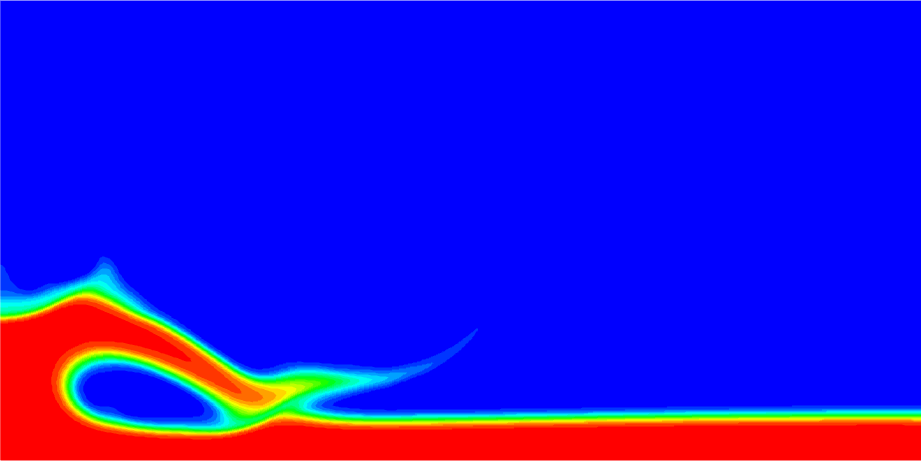
\includegraphics[width=\linewidth]{figure/dambreak/wenojs-8.png}
    \end{subfigure}
    \hfill
    \begin{subfigure}[t]{0.45\linewidth}
        \centering
        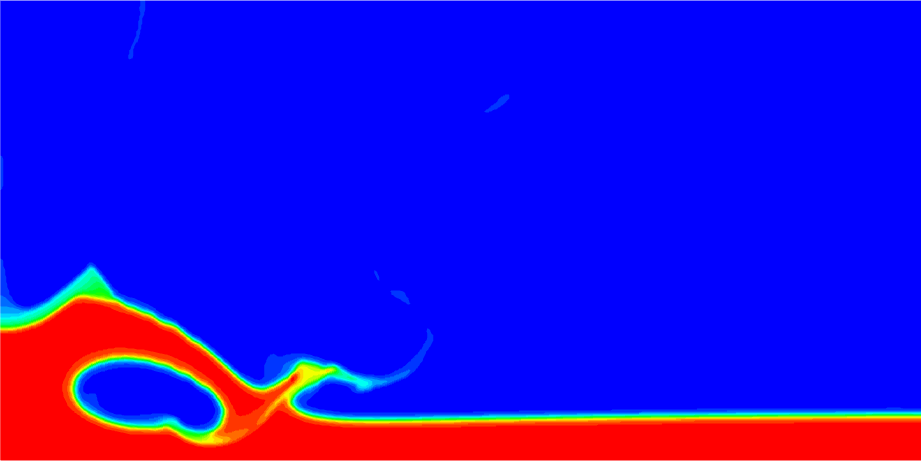
\includegraphics[width=\linewidth]{figure/dambreak/wenoexp1-8.png}
    \end{subfigure}
    \caption{溃坝流问题不同时刻体积分数分布云图
             （左列：WENO-JS；右列：WENO-EXP；网格规模 $200\times 400$）。}
    \label{fig:dambreak_interface}
\end{figure}

\autoref{fig:dambreak_pressure} 给出了压力传感器 $P_s$ 处压力随时间的变化曲线。
两种格式的数值结果均在合理范围内，与实验数据~\cite{LOBOVSKY2014407}吻合良好，
进一步验证了所提格式的准确性与实用性。
此外，在不启用保正限制器的情况下，计算会因界面大变形导致分相密度出现负值而中断，
再次证明了保正算法在含大密度比剧烈两相流问题中的不可或缺性。
% \section{数值结果}

% 本章通过一系列标准算例对所提出格式的精度、鲁棒性及界面捕获能力进行系统验证。
% 所有算例均采用三阶 SSP-RK 格式~\eqref{eq:ssprk}进行时间推进，
% 并结合第~\autoref{sec:pplimiter}节所述的保正限制算法以确保数值解的物理可容许性。
% 为方便叙述，本文涉及的数值格式统一命名如下：
% \begin{itemize}
%     \item \textbf{WENO-JS}：采用基于多项式重构的经典 Jiang--Shu WENO 格式~\cite{JIANG1996}；
%     \item \textbf{WENO-EXP}：本文提出的基于指数多项式逼近空间的 WENO 格式；
% \end{itemize}


% \subsection{MPI并行程序设计}
% 常用的区域分解策略主要有一维条状分解和二维块状分解两种。本文采用一维条状分解，如~\autoref{fig:domain_decomposition_a} 所示，将二维计算域 $\Omega = [x_L, x_R] \times [y_B, y_T]$ 沿 $x$ 方向划分为 $N_p$ 个条状子区域，各进程负责的局部网格规模为 $N_{x,\text{loc}} \times N_y$，其中 $N_{x,\text{loc}} = N_x / N_p$。该分解方式使各进程仅需在 $x$ 方向与相邻进程进行边界数据交换，避免了 $y$ 方向的通信开销。为满足 WENO 重构对邻近单元数据的访问需求，在每个子区域 $x$ 方向的左右边界处各设置宽度为 $r$ 的辅助网格层（ghost cell，$r$ 为模板半宽度），用于存储相邻进程的守恒变量单元平均值，如~\autoref{fig:domain_decomposition_b} 所示。

% 基于上述并行策略，本文采用 C++ 与 MPI 开发了高精度有限体积法并行求解器，其计算流程如~\autoref{fig:weno_algorithm_flow} 所示。
% \begin{figure}[!htbp]
%     \centering
%     \begin{subfigure}[t]{0.45\linewidth}
%         \centering
%         % domin1.tex
% 沿 x 方向的一维条状区域分解示意图（以 N_p = 3 为例）
% Requires: \usetikzlibrary{arrows.meta}

\begin{tikzpicture}[
    scale=0.42,
    every node/.style={font=\small},
    gridline/.style={gray!60, very thin},
    proclabel/.style={font=\Large\bfseries, text=brown!70!black}
]

% 参数：总网格 12x9，分成 3 个进程（每个进程 4 列）
\def\Nx{12}
\def\Ny{9}
\def\NxLoc{4}   % 12/3 = 4

% 填充三个进程区域（不同颜色）
\fill[red!70,    opacity=0.85] (0,0)         rectangle (\NxLoc,   \Ny);
\fill[blue!60,   opacity=0.85] (\NxLoc,0)    rectangle (2*\NxLoc, \Ny);
\fill[yellow!80, opacity=0.85] (2*\NxLoc,0)  rectangle (3*\NxLoc, \Ny);

% 绘制网格线
\foreach \x in {0,...,\Nx} {
    \draw[gridline] (\x,0) -- (\x,\Ny);
}
\foreach \y in {0,...,\Ny} {
    \draw[gridline] (0,\y) -- (\Nx,\y);
}

% 绘制子区域之间的粗分界线
\foreach \k in {1,2} {
    \draw[very thick, black] (\k*\NxLoc,0) -- (\k*\NxLoc,\Ny);
}
% 外框
\draw[very thick, black] (0,0) rectangle (\Nx,\Ny);

% 进程标号
\node[proclabel] at (0.5*\NxLoc, 0.5*\Ny) {\small 进程 1};
\node[proclabel] at (1.5*\NxLoc, 0.5*\Ny) {\small 进程 2};
\node[proclabel] at (2.5*\NxLoc, 0.5*\Ny) {\small 进程 3};

% 坐标轴
% \draw[-{Stealth[length=2mm]}, thick] (-1.2,-1.2) -- (1.8,-1.2) node[right] {$x$};
% \draw[-{Stealth[length=2mm]}, thick] (-1.2,-1.2) -- (-1.2,1.8) node[above] {$y$};

% 边界坐标
% \node[below] at (0,-0.2)   {\small $x_L$};
% \node[below] at (\Nx,-0.2) {\small $x_R$};
% \node[left]  at (-0.1,0)   {\small $y_B$};
% \node[left]  at (-0.1,\Ny) {\small $y_T$};

\end{tikzpicture}
%         \caption{一维条状区域分解}
%         \label{fig:domain_decomposition_a}
%     \end{subfigure}
%     \hfill
%     \begin{subfigure}[t]{0.45\linewidth}
%         \centering
%         % domin2.tex（与 domin1 行列参数对齐）
\begin{tikzpicture}[
    scale=0.42,
    every node/.style={font=\small},
    gridline/.style={gray!60, very thin},
    proclabel/.style={font=\normalsize\bfseries, text=brown!70!black},
    arrowstyle/.style={-{Stealth[length=2.5mm]}, thick, purple!70!black}
]

\def\r{3}        % 辅助层列数
\def\NxL{4}      % 内部单元列数（与 domin1 单进程宽度一致）
\def\NyL{9}      % 行数（与 domin1 完全一致）

% 辅助网格层（灰色）
\fill[gray!40, opacity=0.85] (0,0)        rectangle (\r,       \NyL);
\fill[gray!40, opacity=0.85] (\r+\NxL,0)  rectangle (2*\r+\NxL,\NyL);

% 内部单元（蓝色，与 domin1 进程2 完全一致）
\fill[blue!60, opacity=0.85] (\r,0) rectangle (\r+\NxL, \NyL);

% 网格线
\foreach \x in {0,...,10} {
    \draw[gridline] (\x,0) -- (\x,\NyL);
}
\foreach \y in {0,...,\NyL} {
    \draw[gridline] (0,\y) -- (2*\r+\NxL,\y);
}

% 分隔粗线
\draw[very thick, black] (\r,0)      -- (\r,\NyL);
\draw[very thick, black] (\r+\NxL,0) -- (\r+\NxL,\NyL);
% 外框
\draw[very thick, black] (0,0) rectangle (2*\r+\NxL, \NyL);

% 标注
\node[proclabel] at (\r+0.5*\NxL, 0.5*\NyL) {\small 本进程};

% 通信箭头
\draw[arrowstyle] (-1.8, \NyL/2+0.8) -- (0.4, \NyL/2+0.8)
    node[midway, above, font=\footnotesize, text=black] {接收};
\draw[arrowstyle] (\r+0.4, \NyL/2-0.8) -- (-1.8, \NyL/2-0.8)
    node[midway, above, font=\footnotesize, text=black] {发送};
\draw[arrowstyle] (\r+\NxL-0.4, \NyL/2+0.8) -- (2*\r+\NxL+1.8, \NyL/2+0.8)
    node[midway, above, font=\footnotesize, text=black] {发送};
\draw[arrowstyle] (2*\r+\NxL+1.8, \NyL/2-0.8) -- (\r+\NxL+0.4, \NyL/2-0.8)
    node[midway, above, font=\footnotesize, text=black] {接收};


\end{tikzpicture}
%         \caption{辅助网格层与通信示意.蓝色网格为本进程负责的计算区域，灰色网格为辅助网格层，箭头表示通信数据流向}
%         \label{fig:domain_decomposition_b}
%     \end{subfigure}
%     \caption{沿 $x$ 方向的一维条状区域分解与进程间通信示意图}
%     \label{fig:domain_decomposition}
% \end{figure}
% \begin{figure}[!htbp]
%     \centering
%     % ============================================================
%  MPI 并行计算流程图
%  描述：基于 WENO 重构 + 保正限制器 + SSP-RK 时间推进
%        的 MPI 并行求解器主循环结构
%
%  三栏布局：
%    左栏  —— 主进程控制流程（时间推进主循环）    主题色：绿
%    中栏  —— MPI 通信层（非阻塞辅助层数据交换）  主题色：蓝
%    右栏  —— 各进程本地计算流程                  主题色：红
%
%  颜色层次（同色系，由深到浅）：
%    文本框填充  > 背景分区框填充
%    绿: green!15  >  green!6
%    蓝: blue!12   >  blue!5
%    红: red!10    >  red!4
% ============================================================

\tikzset{
  % 开始/结束圆角端子框（左栏，绿色系）
  terminal/.style={
    draw=green!55!black, fill=white,
    rounded corners=12pt,
    align=center, font=\small\bfseries,
    minimum height=0.75cm, minimum width=2.6cm,
    inner sep=5pt, line width=1.0pt
  },
  % 通用流程框（左栏，绿色系）
  mainbox/.style={
    draw=green!55!black, fill=white,
    align=center, font=\small,
    minimum height=0.85cm, minimum width=2.8cm,
    inner sep=5pt, line width=1.0pt
  },
  % 判断菱形框（左栏，绿色系）
  decision/.style={
    draw=green!55!black, fill=white,
    diamond, aspect=2.6,
    align=center, font=\small,
    inner sep=2pt, line width=1.0pt
  },
  % MPI 通信操作框（中栏，蓝色系）
  mpibox/.style={
    draw=blue!60, fill=white,
    align=center, font=\small,
    minimum height=1.1cm, minimum width=2.8cm,
    inner sep=5pt, line width=1.0pt
  },
  % 本地计算步骤框（右栏，红色系）
  compbox/.style={
    draw=red!60!black, fill=white,
    align=center, font=\small,
    minimum height=0.85cm, minimum width=3.0cm,
    inner sep=5pt, line width=1.0pt
  },
  % 有向箭头样式
  arr/.style={->, >=Stealth, thick},
}

\resizebox{0.8\textwidth}{!}{%
\begin{tikzpicture}[node distance=0.65cm]

% ══════════════════════════════════════════════════════════
%  左栏：主进程时间推进主循环
%  流程：初始化 → 启动子步计算 → 更新时间与解 → 判断终止
% ══════════════════════════════════════════════════════════

% 程序入口
\node[terminal] (start) {开始};

% 初始化各单元均值 Q^0_{i,j}（包括初始条件赋值与边界条件设置）
\node[mainbox, below=0.6cm of start] (init) {
  初始化 $\overline{\bm{Q}}_{i,j}^0$
};

% 启动 SSP-RK 子步：触发 MPI 辅助层数据交换与本地 WENO 计算
% 此框为当前子步的"发起"节点，实际 ΔQ 由右栏计算完成后返回
\node[mainbox, below=0.6cm of init] (calcdQ) {
  发起 SSP-RK 子步计算
};

% 接收本地计算结果，更新物理时间与守恒变量
\node[mainbox, below=0.6cm of calcdQ] (update) {
  $t \leftarrow t + \Delta t$\\[-2pt]
  {\footnotesize $\bm{Q} \leftarrow \bm{Q} + \Delta\bm{Q}$}
};

% 时间终止判断：t ≥ T 则退出，否则继续下一子步
\node[decision, below=0.65cm of update] (tcheck) {
  $t \geq T$?
};

% 程序出口
\node[terminal, below=0.7cm of tcheck] (end) {结束};

% ══════════════════════════════════════════════════════════
%  中栏：MPI 通信层
%  采用非阻塞通信（Isend/Irecv）与内部单元计算重叠，
%  降低通信等待开销；Waitall 确保辅助数据就绪后再重构
% ══════════════════════════════════════════════════════════

% 发起非阻塞辅助层数据交换
\node[mpibox, right=2.2cm of calcdQ] (isend) {
  发起非阻塞辅助层数据交换
};

% 等待所有非阻塞通信完成，确保辅助数据更新完毕
\node[mpibox, below=0.6cm of isend] (waitall) {
  等待通信完成
};

% ══════════════════════════════════════════════════════════
%  右栏：各 MPI 进程本地计算流程
%  顺序：内部单元重构（与通信重叠） → 等待辅助 →
%        边界单元重构 → 保正限制器 → 通量计算 → RK 更新
% ══════════════════════════════════════════════════════════

% 第一步：对内部单元（不依赖辅助）进行 WENO 重构
% 与 MPI 通信重叠执行，隐藏通信延迟
\node[compbox, right=2.0cm of isend] (weno_int) {
  内部单元 WENO 重构\\[-1pt]
  {\footnotesize （与辅助层通信重叠执行）}
};

% 第二步：辅助数据就绪后，对边界单元进行 WENO 重构
\node[compbox] (weno_bnd) at (weno_int |- waitall) {
  边界单元 WENO 重构\\[-1pt]
  {\footnotesize （依赖辅助数据）}
};

% 第三步：施加保正限制器，确保分密度等物理量非负
\node[compbox, below=0.6cm of weno_bnd] (limiter) {
  施加保正限制器\\[-1pt]
  {\footnotesize （确保 $\rho_k > 0$，$p > 0$）}
};

% 第四步：利用重构界面值计算数值通量（如 HLLC / Lax-Friedrichs）
\node[compbox, below=0.6cm of limiter] (flux) {
  计算界面数值通量\\[-1pt]
  {\footnotesize （HLLC / Lax-Friedrichs）}
};

% 第五步：按 SSP-RK 格式累加空间残差，得到本子步的 ΔQ
\node[compbox, below=0.6cm of flux] (rk) {
  有限体积法残差累加\\[-1pt]
  {\footnotesize （输出 $\Delta\bm{Q}$ 至主流程）}
};

% ══════════════════════════════════════════════════════════
%  背景分区框：三列分别用绿/蓝/红虚线框标注
%  使用 on background layer 避免覆盖前景节点
%  两次绘制：第一次用 fit 节点确定各列宽度，
%            第二次统一拉齐上下边界至 start/rk 水平
% ══════════════════════════════════════════════════════════
\begin{scope}[on background layer]
  % 第一次：用 fit 获取各列的左右范围（宽度锚点）
  \node[
    draw=green!55!black, fill=green!6,
    rounded corners=8pt, dashed, line width=1.1pt,
    fit=(start)(init)(calcdQ)(update)(tcheck)(end),
    inner sep=12pt
  ] (leftframe) {};

  \node[
    draw=blue!60, fill=blue!5,
    rounded corners=8pt, dashed, line width=1.1pt,
    fit=(isend)(waitall),
    inner sep=12pt
  ] (midframe) {};

  \node[
    draw=red!60!black, fill=red!4,
    rounded corners=8pt, dashed, line width=1.1pt,
    fit=(weno_int)(weno_bnd)(limiter)(flux)(rk),
    inner sep=12pt
  ] (rightframe) {};
\end{scope}

% 第二次：以 start 顶部与 rk 底部为统一上下边界，重绘三框
\begin{scope}[on background layer]
  % 统一上下边界坐标
  \coordinate (top_y) at ($(start.north) + (0,  0.42cm)$);
  \coordinate (bot_y) at ($(rk.south)    + (0, -0.42cm)$);

  % 左框（主流程）：绿色虚线
  \filldraw[fill=green!6, draw=green!55!black,
            rounded corners=8pt, dashed, line width=1.1pt]
    (leftframe.west  |- top_y) rectangle (leftframe.east  |- bot_y);

  % 中框（MPI 通信）：蓝色虚线
  \filldraw[fill=blue!5, draw=blue!60,
            rounded corners=8pt, dashed, line width=1.1pt]
    (midframe.west   |- top_y) rectangle (midframe.east   |- bot_y);

  % 右框（本地计算）：红色虚线
  \filldraw[fill=red!4, draw=red!60!black,
            rounded corners=8pt, dashed, line width=1.1pt]
    (rightframe.west |- top_y) rectangle (rightframe.east |- bot_y);
\end{scope}

% 分区标签（位于各框顶部正中）
\node[font=\small\bfseries, text=green!60!black]
  at (leftframe.north  |- top_y) [above=4pt] {主流程};
\node[font=\small\bfseries, text=blue!65!black]
  at (midframe.north   |- top_y) [above=4pt] {MPI 通信};
\node[font=\small\bfseries, text=red!65!black]
  at (rightframe.north |- top_y) [above=4pt] {各进程本地计算};

% ══════════════════════════════════════════════════════════
%  有向箭头：连接各节点，表示控制流与数据流
% ══════════════════════════════════════════════════════════

% ── 左栏内部纵向连接 ──
\draw[arr] (start)  -- (init);
\draw[arr] (init)   -- (calcdQ);
\draw[arr] (update) -- (tcheck);
% t ≥ T：向下退出
\draw[arr] (tcheck) -- node[right, font=\small] {是} (end);
% t < T：从 tcheck 左侧折回 calcdQ，进入下一时间子步
\draw[arr] (tcheck.west)
  -- node[above, font=\small] {否}
  ++(-1.5cm, 0)
  |- (calcdQ.west);

% ── 左栏 → 中栏：启动子步计算时触发非阻塞通信 ──
\draw[arr] (calcdQ.east) -- (isend.west);

% ── 中栏 → 右栏：发起通信的同时，立即启动内部单元重构 ──
\draw[arr] (isend.east) -- (weno_int.west);

% ── 右栏内部：内部重构完成后等待通信，再处理边界单元 ──
% weno_int 底部向下，折向 waitall 顶部（表示"等待"依赖关系）
\draw[arr] (weno_int.south)
  -- ++(0, -0.3cm)
  -| (waitall.north);

% ── 中栏 → 右栏：辅助数据就绪，触发边界单元重构 ──
\draw[arr] (waitall.east) -- (weno_bnd.west);

% ── 右栏内部纵向连接：重构 → 限制器 → 通量 → RK更新 ──
\draw[arr] (weno_bnd) -- (limiter);
\draw[arr] (limiter)  -- (flux);
\draw[arr] (flux)     -- (rk);

% ── 右栏 → 左栏：子步计算完成，将 ΔQ 返回主流程 ──
% 从 rk 左侧引出，经底部通道折回 update 右侧
\draw[arr] (rk.west)
  -- ++(-7cm, 0)
  |- (update.east);

\end{tikzpicture}
}
%     \caption{基于非多项式 WENO 重构的并行求解器计算流程示意图}
%     \label{fig:weno_algorithm_flow}
% \end{figure}


% 为评估该求解器的性能，选取二维 XXX 算例\footnote{请替换为你实际采用的测试算例名称，例如二维 Riemann 问题、溃坝问题等。}作为测试对象，计算网格规模为 $N_x \times N_y = \text{XXX} \times \text{XXX}$，在同一台多核计算节点上分别采用 $N_p = 1, 2, 4, 8, 16, 32$ 个 MPI 进程运行至相同的物理时刻。定义并行加速比与并行效率分别为：
% \begin{equation}
%     S_{N_p} = \frac{T_1}{T_{N_p}}, \qquad
%     E_{N_p} = \frac{S_{N_p}}{N_p} \times 100\%,
% \end{equation}
% 其中 $T_1$ 为单进程（串行）运行的墙钟时间，$T_{N_p}$ 为采用 $N_p$ 个进程并行运行的墙钟时间。测试结果如表~\autoref{tab:parallel_performance} 所示。

% \begin{table}[!htbp]
%     \centering
%     \caption{MPI 并行程序的加速比与并行效率测试结果}
%     \label{tab:parallel_performance}
%     \begin{tabular}{ccccc}
%         \toprule
%         进程数 $N_p$ & 墙钟时间 $T_{N_p}$ (s) & 加速比 $S_{N_p}$ & 并行效率 $E_{N_p}$ (\%) \\
%         \midrule
%         1  & --  & 1.00  & 100.0 \\
%         2  & --  & --    & --    \\
%         4  & --  & --    & --    \\
%         8  & --  & --    & --    \\
%         16 & --  & --    & --    \\
%         32 & --  & --    & --    \\
%         \bottomrule
%     \end{tabular}
% \end{table}

% 由表~\autoref{tab:parallel_performance} 可见，随着进程数的增加，程序的墙钟时间显著下降，加速比接近于理想线性加速。在进程数较少时，并行效率维持在较高水平；当进程数进一步增加时，并行效率有所下降，但整体仍保持在可接受范围内。该结果表明，本文所采用的区域分解策略与通信-计算重叠机制能够有效地屏蔽通信延迟，所实现的并行程序具有良好的可扩展性。

% \subsection{一维光滑对流问题}
% \label{sec:1D_smooth_advection}

% 本算例考虑具有光滑初始条件的一维三方程模型~\eqref{eq:governing}，
% 初始体积分数场设置为
% \begin{equation}
%     z_1(x, 0) = (0.5 - \varepsilon_z)\sin(2\pi x) + 0.5,
% \end{equation}
% 其中 $\varepsilon_z = 10^{-2}$。其余初始条件设置为：
% $\rho_1(x, 0) = 1.2~\mathrm{kg/m^3}$，$\rho_2(x, 0) = 1~\mathrm{kg/m^3}$，
% $u(x, 0) = 1~\mathrm{m/s}$，$p(x, 0) = 0~\mathrm{Pa}$，
% 人工声速取为 $c_1 = c_2 = 1~\mathrm{m/s}$。
% 计算域为 $x \in [0, 1]$，输出时间为 $t = 1~\mathrm{s}$，
% 采用周期性边界条件，时间步长取 $\Delta t = 10\Delta x^2$。

% 表~\autoref{tab:1d_smooth_compare} 列出了采用 WENO-JS、WENO-EXP在不同网格分辨率下的数值误差与收敛阶数。结果表明，WENO-JS 格式均达到五阶收敛精度 而和 WENO-EXP-I 格式达到实现了六阶收敛精度，验证了所提出格式在光滑流场中的高阶精度。

% \begin{table}[!ht]
%     \centering
%     \caption{一维光滑对流问题体积分数 $z_1$ 的数值误差与收敛阶对比（$t = 1~\mathrm{s}$）}
%     \label{tab:1d_smooth_compare}
%     \begin{tabular}{ccccccccc}
%         \toprule
%         & \multicolumn{4}{c}{WENO-JS} & \multicolumn{4}{c}{WENO-EXP} \\
%         \cmidrule(lr){2-5} \cmidrule(lr){6-9}
%         $N$ 
%         & $L^\infty$ 误差 & 收敛阶 
%         & $L^1$ 误差 & 收敛阶
%         & $L^\infty$ 误差 & 收敛阶 
%         & $L^1$ 误差 & 收敛阶 \\
%         \midrule
%         20  & 2.57E-03 & --   & 1.71E-03 & --   & 2.57E-03 & --   & 1.71E-03 & --   \\
%         40  & 8.81E-05 & 4.87 & 4.96E-05 & 5.11 & 8.81E-05 & 4.87 & 4.96E-05 & 5.11 \\
%         80  & 2.73E-06 & 5.01 & 1.47E-06 & 5.07 & 2.73E-06 & 5.01 & 1.47E-06 & 5.07 \\
%         160 & 8.34E-08 & 5.03 & 4.46E-08 & 5.04 & 8.34E-08 & 5.03 & 4.46E-08 & 5.04 \\
%         320 & 2.43E-09 & 5.10 & 1.37E-09 & 5.03 & 2.43E-09 & 5.10 & 1.37E-09 & 5.03 \\
%         \bottomrule
%     \end{tabular}
% \end{table}
% \begin{remark}
%     对于上述光滑初始体积分数，$z_1$ 的三阶导数与五阶导数之比为常数,与空间坐标 $x$ 及参数 $\varepsilon_z$ 均无关，具体地，
%     \begin{equation}
%         \frac{z_1^{(5)}}{z_1^{(3)}}
%         = \frac{-32\pi^5\cos(2\pi x)(\varepsilon_z - 1/2)}{8\pi^3\cos(2\pi x)(\varepsilon_z - 1/2)}
%         = -4\pi^2.
%     \end{equation}
%     这一特殊性质使得本算例可同时用于验证格式中 $\lambda^2\Delta x^2$ 项的数值计算结果与解析结果的一致性，相应的验证结果见~\autoref{fig:1D_smooth_result}。
% \end{remark}

% \begin{figure}[!htbp]
%     \centering
%     \begin{subfigure}[t]{0.45\linewidth}
%         \centering
%         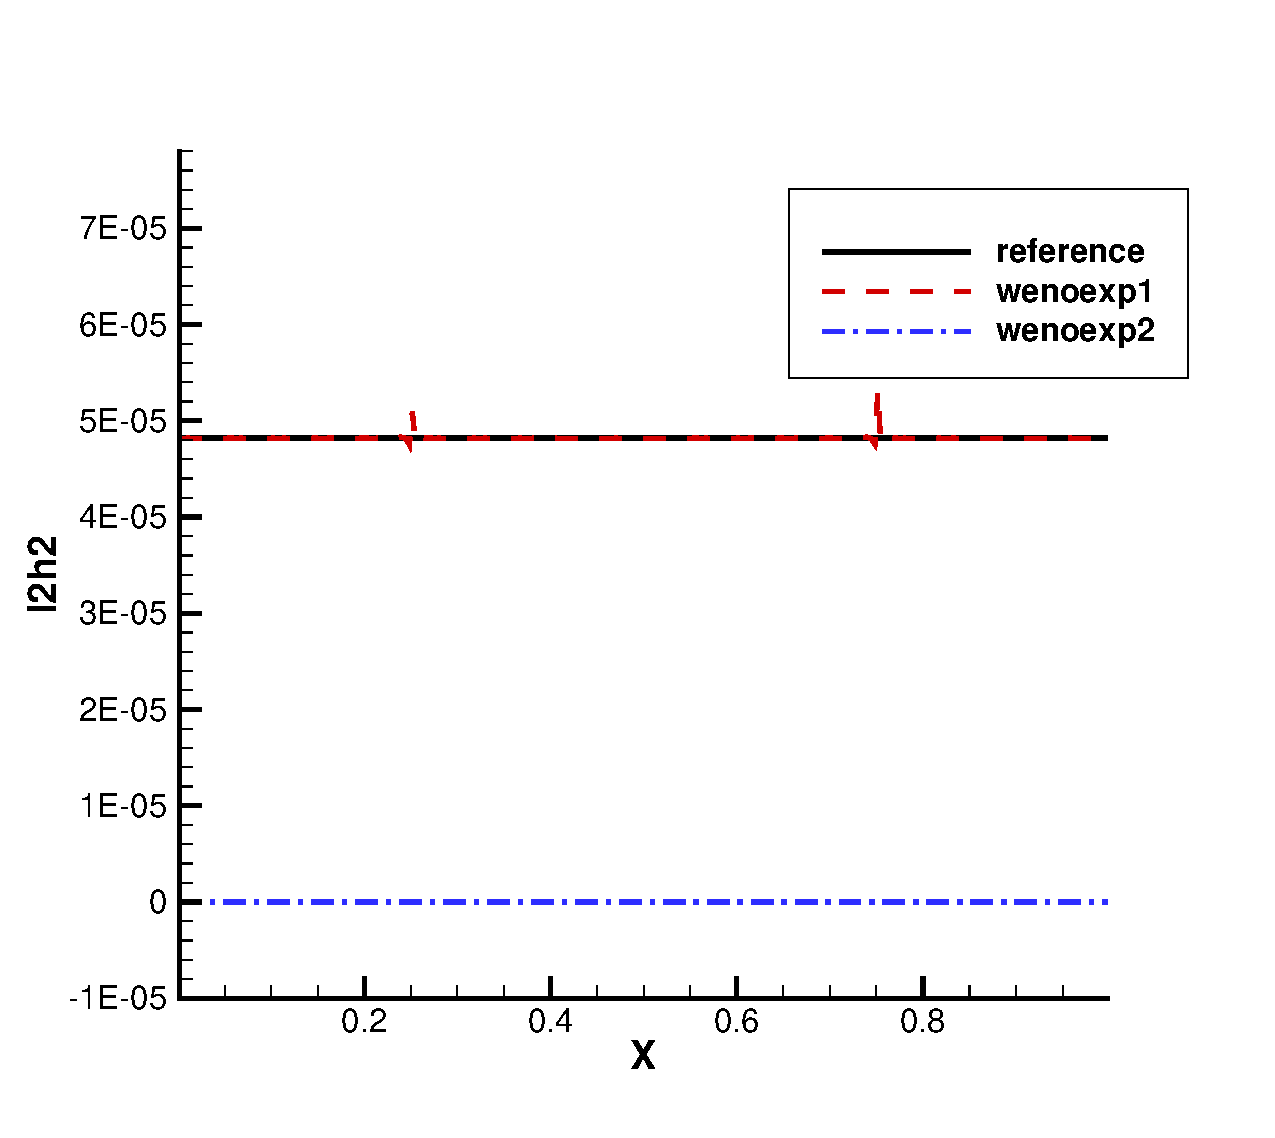
\includegraphics[width=\linewidth]{figure/1D-smooth/l2h2.eps}
%         \caption{l2h2 分布图}
%     \end{subfigure}
%     \hfill
%     \begin{subfigure}[t]{0.45\linewidth}
%         \centering
%         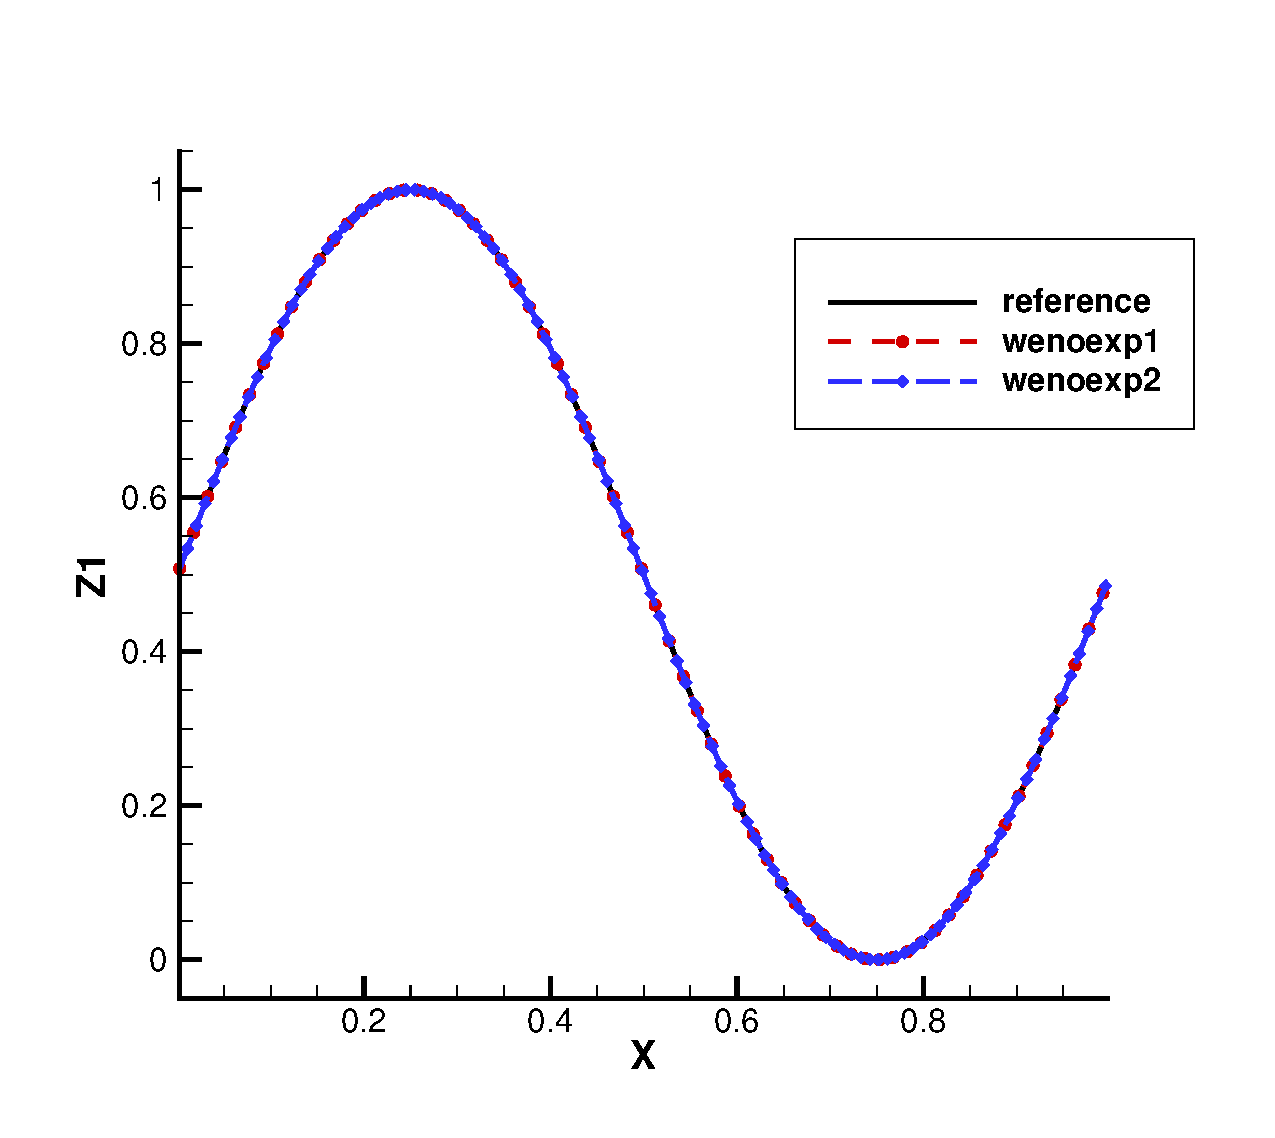
\includegraphics[width=\linewidth]{figure/1D-smooth/z1.eps}
%         \caption{数值解 $z_1$ 的分布图}
%     \end{subfigure}
%     \caption{一维光滑对流问题的数值结果}
%     \label{fig:1D_smooth_result}
% \end{figure}

% \subsection{一维锐利对流问题}

% 本算例用于验证所提格式在含有锐利相界面的一维弱可压两相流模拟中
% 保持无振荡特性的能力。初始体积分数场设置为
% \begin{equation}
%     z_1(x, 0) = \begin{cases}
%         1 - \varepsilon_z, & x \in (0.25,\, 0.75), \\
%         \varepsilon_z,     & \text{其他},
%     \end{cases}
% \end{equation}
% 其中 $\varepsilon_z = 10^{-10}$，以模拟近乎纯相的两相界面。
% 其余参数设置为：
% $\rho_1(x, 0) = 1000~\mathrm{kg/m^3}$，$\rho_2(x, 0) = 1~\mathrm{kg/m^3}$，
% $u(x, 0) = 1~\mathrm{m/s}$，$p(x, 0) = 0~\mathrm{Pa}$，
% $c_1 = c_2 = 70~\mathrm{m/s}$。
% 计算域为 $x \in [0, 1]$，网格数取 $N = 200$，
% 采用周期性边界条件，输出时间为 $t = 1~\mathrm{s}$。

% \autoref{fig:z1} 给出了体积分数 $z_1$ 的数值结果，\autoref{fig:z1-large} 为界面附近的局部放大图。且 WENO-EXP 格式在界面附近引入的数值耗散更小，所得界面厚度更薄。
% \begin{figure}[!htbp]
%     \centering
%     \begin{subfigure}[t]{0.45\linewidth}
%         \centering
%         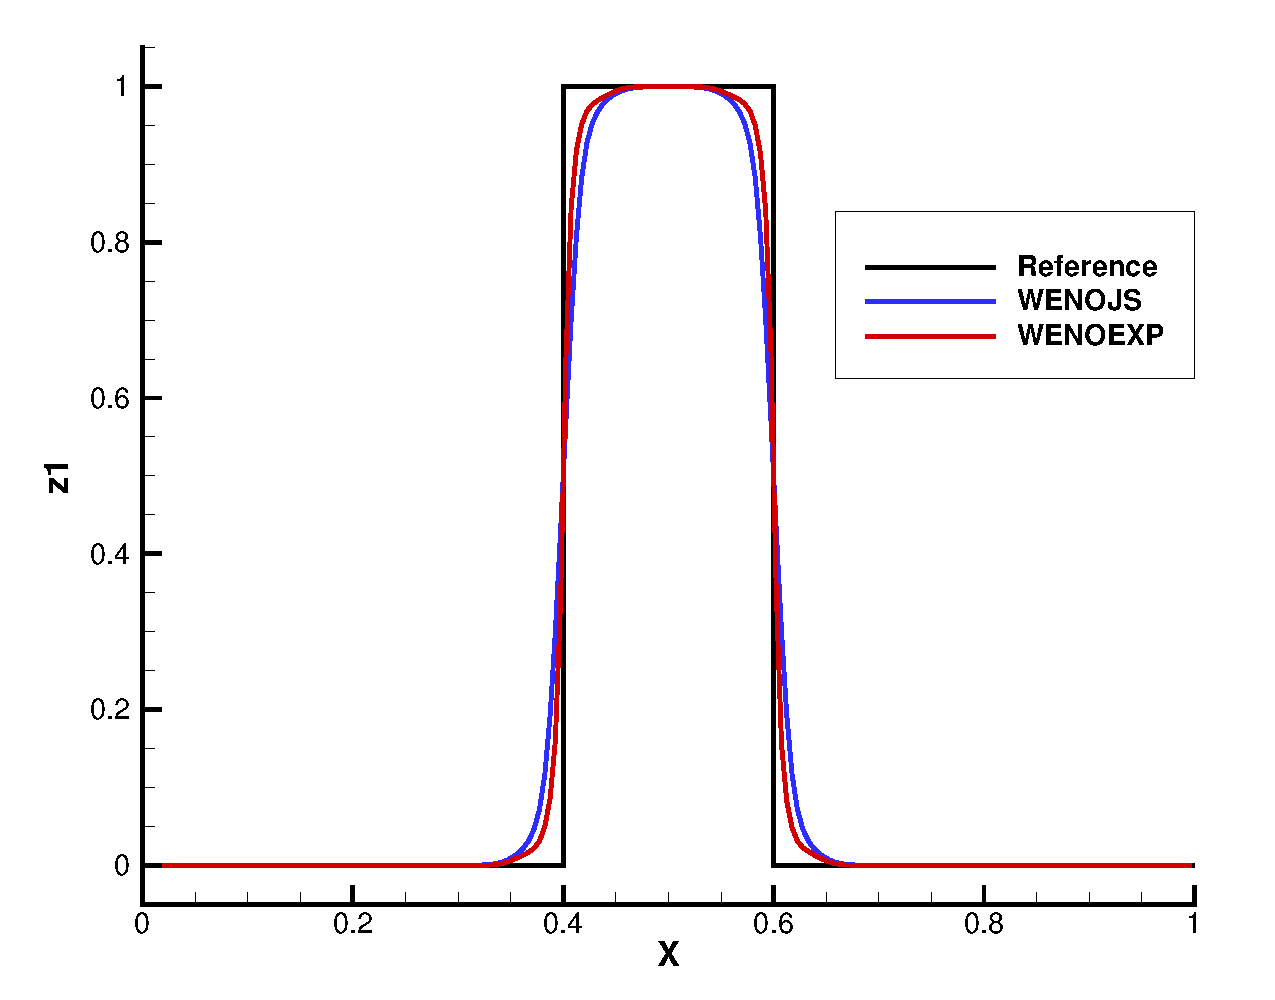
\includegraphics[width=\linewidth]{figure/1D-sharp/z1.eps}
%         \caption{整体视图}
%         \label{fig:z1}
%     \end{subfigure}
%     \hfill
%     \begin{subfigure}[t]{0.45\linewidth}
%         \centering
%         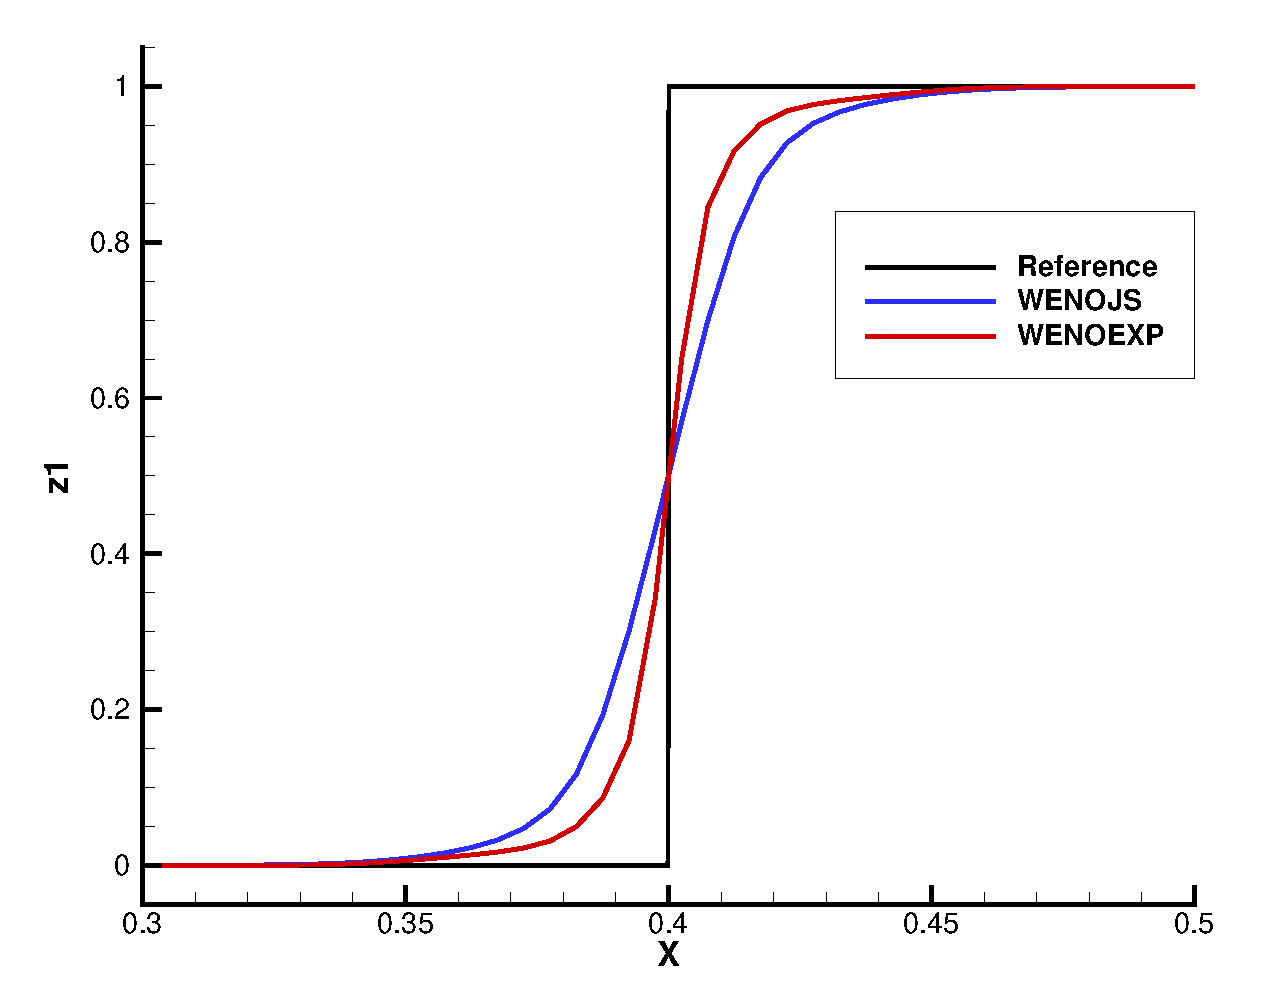
\includegraphics[width=\linewidth]{figure/1D-sharp/z1-large.eps}
%         \caption{局部放大视图}
%         \label{fig:z1-large}
%     \end{subfigure}
%     \caption{一维锐利界面平流问题中 WENO-JS 与 WENO-EXP 格式计算所得体积分数分布。}
% \end{figure}

% % \begin{figure}[!htbp]
% %     \centering
% %     \label{fig:}
% %     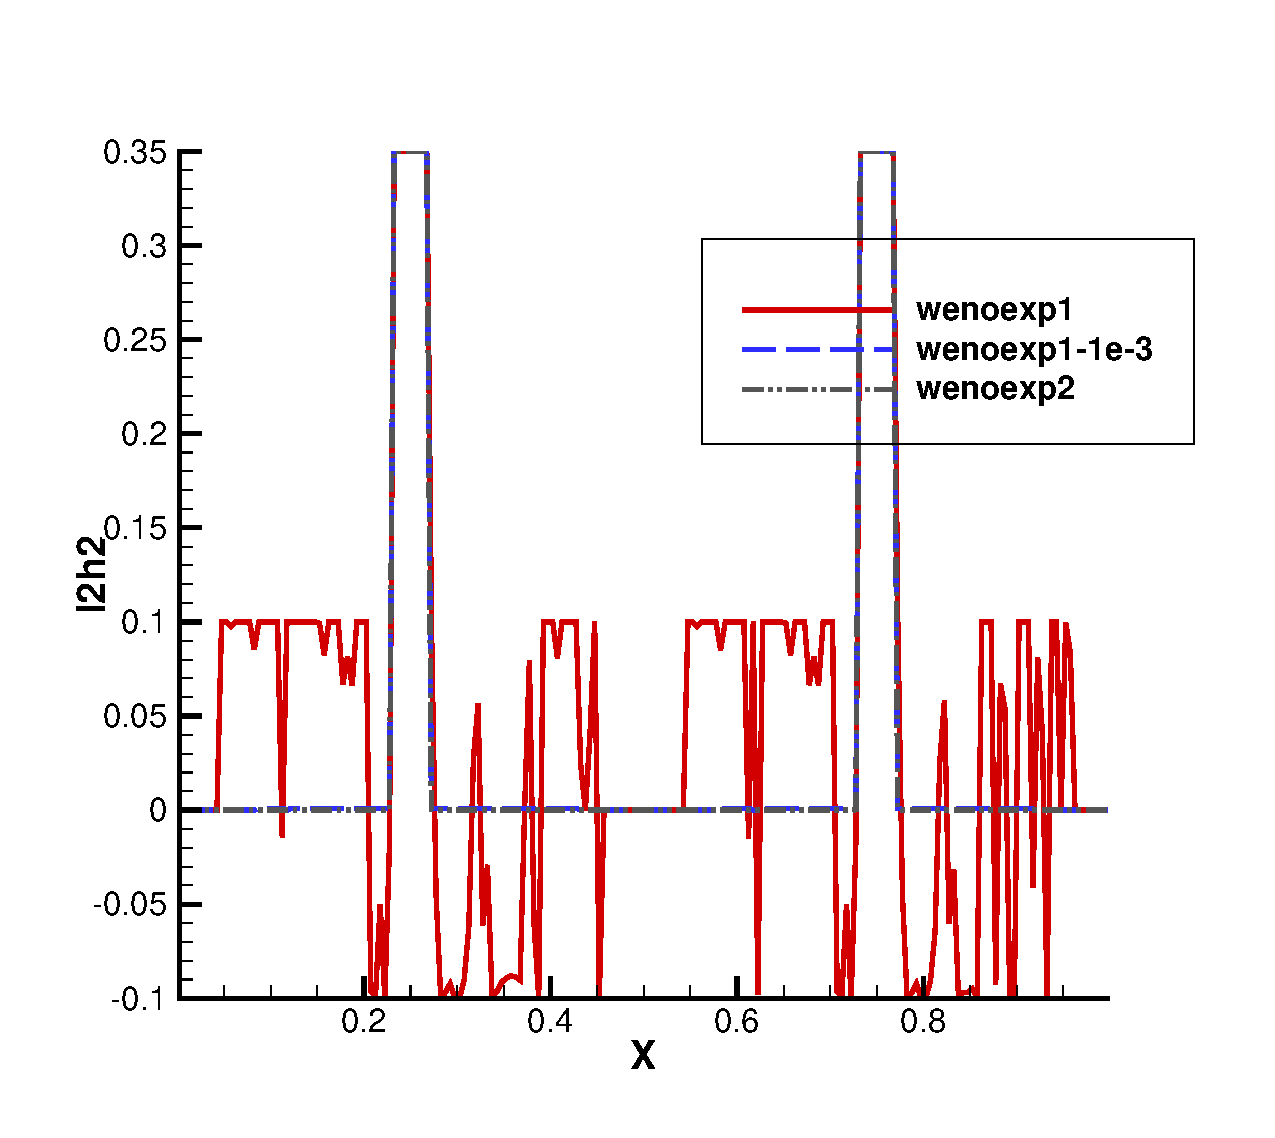
\includegraphics[width=0.7\linewidth]{figure/1D-sharp/l2h2.eps}
% %     \caption{这个似乎是因为lambda=0.1这个太大了，导致会产生振荡，扩散到0到1整个计算区域，从而大部分的地方就爆了.在算升阶l2h2的时候，lambda取1e-3就不会有这个问题了.}
% % \end{figure}
% \autoref{fig:1D_sharp_oscillation} 展示了 WENO-EXP 格式在不同重构变量下计算的数值振荡情况。结果表明，与采用 conv 和 prim1 重构的格式相比，采用 char 和 prim2 重构的格式所产生的振荡幅度显著更小，改善幅度达 $5{\sim}7$ 个数量级。
% \begin{figure}[!htbp]
%     \centering
%     \begin{subfigure}[t]{0.45\linewidth}
%         \centering
%         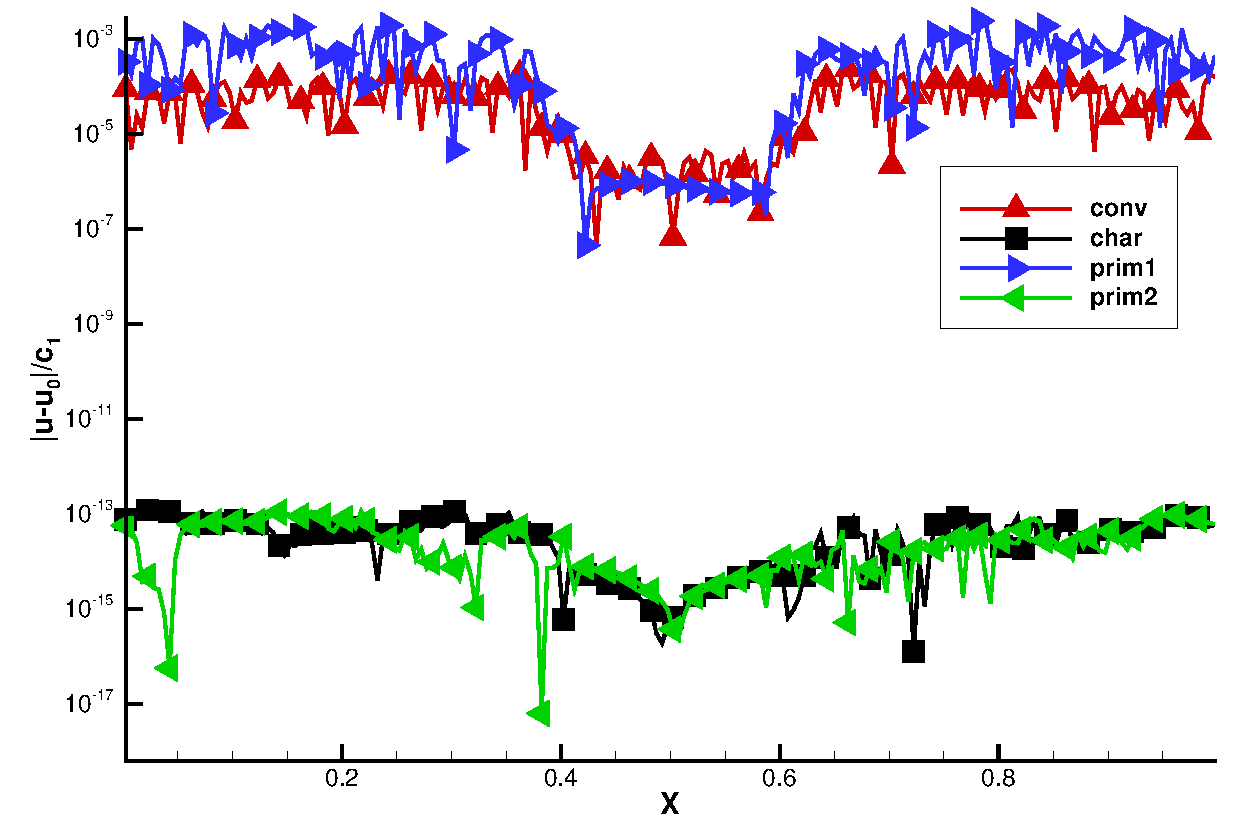
\includegraphics[width=\linewidth]{figure/1D-sharp/speed-eps-converted-to.pdf}
%         \caption{速度}
%     \end{subfigure}
%     \hfill
%     \begin{subfigure}[t]{0.45\linewidth}
%         \centering
%         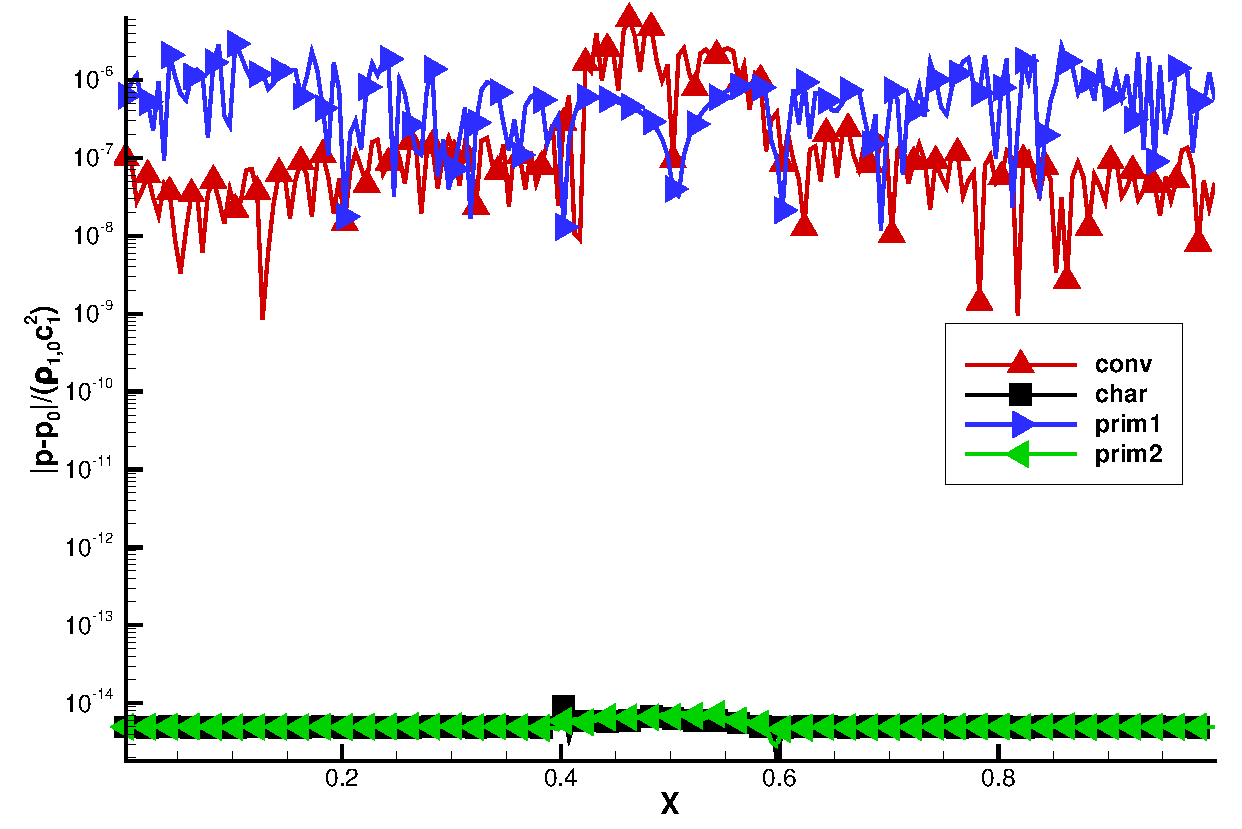
\includegraphics[width=\linewidth]{figure/1D-sharp/pre-eps-converted-to.pdf}
%         \caption{压力}
%     \end{subfigure}
%     \caption{采用不同重构变量的WENO-EXP格式对一维锐利界面平流问题的数值振荡计算结果。}
%     \label{fig:1D_sharp_oscillation}
% \end{figure}


% \subsection{二维光滑对流问题}

% 本算例将精度测试推广至二维情形。初始体积分数场设置为
% \begin{equation}
%     z_1(x, y, 0) = (0.5 - \varepsilon_z)\sin(2\pi(x + y)) + 0.5,
%     \quad (x, y) \in [0, 1] \times [0, 1],
% \end{equation}
% 其余参数与第~\autoref{sec:1D_smooth_advection}节相同。

% \begin{table}[!ht]
%     \centering
%     \caption{\textcolor{red}{一维光滑对流问题体积分数 $z_1$ 的数值误差与收敛阶对比（$t = 1~\mathrm{s}$）}}
%     \label{tab:2d_smooth_compare}
%     \begin{tabular}{ccccccccc}
%         \toprule
%         & \multicolumn{4}{c}{WENO-JS} & \multicolumn{4}{c}{WENO-EXP} \\
%         \cmidrule(lr){2-5} \cmidrule(lr){6-9}
%         $N$ 
%         & $L^\infty$ 误差 & 收敛阶 
%         & $L^1$ 误差 & 收敛阶
%         & $L^\infty$ 误差 & 收敛阶 
%         & $L^1$ 误差 & 收敛阶 \\
%         \midrule
%         20  & 2.57E-03 & --   & 1.71E-03 & --   & 2.57E-03 & --   & 1.71E-03 & --   \\
%         40  & 8.81E-05 & 4.87 & 4.96E-05 & 5.11 & 8.81E-05 & 4.87 & 4.96E-05 & 5.11 \\
%         80  & 2.73E-06 & 5.01 & 1.47E-06 & 5.07 & 2.73E-06 & 5.01 & 1.47E-06 & 5.07 \\
%         160 & 8.34E-08 & 5.03 & 4.46E-08 & 5.04 & 8.34E-08 & 5.03 & 4.46E-08 & 5.04 \\
%         320 & 2.43E-09 & 5.10 & 1.37E-09 & 5.03 & 2.43E-09 & 5.10 & 1.37E-09 & 5.03 \\
%         \bottomrule
%     \end{tabular}
% \end{table}

% 表~\autoref{tab:2d_smooth_compare} 列出了 WENO-JS 和 WENO-EXP 格式在二维光滑对流问题中的数值误差与收敛阶数。结果表明，WENO-JS 格式保持五阶收敛精度，而 WENO-EXP 格式实现了预期的六阶收敛精度，与一维情形的结论相一致。

% % \subsection{二维多相涡旋对流问题}

% % 一维算例中具有高阶收敛性质的数值格式，在多维情形下未必能维持同等收敛阶数~\cite{li2020finite}。
% % 为此，本算例通过二维多相涡旋对流问题对格式的二维收敛性能进行评估，
% % 该问题的解析解见附录~B。

% % 在周期性计算域 $[-L, L] \times [-L, L]$（$L = 1~\mathrm{m}$）内，
% % 初始条件设置为
% % \begin{equation}
% %     z_1(r, \theta, 0) = (1 - 2\varepsilon_\alpha)\exp\!\left(-\frac{r^2}{r_0^2}\right) + \varepsilon_\alpha,
% % \end{equation}
% % \begin{equation}
% %     p(r, \theta, 0) = P\left(1 - \exp\!\left(-\frac{r^2}{r_0^2}\right)\right),
% % \end{equation}
% % \begin{equation}
% %     u(r, \theta, 0) = U - \sin\theta\sqrt{\frac{r}{\rho}\frac{\partial p}{\partial r}}, \qquad v(r, \theta, 0) = V + \cos\theta\sqrt{\frac{r}{\rho}\frac{\partial p}{\partial r}},
% % \end{equation}
% % 其中 $r$ 和 $\theta$ 为柱坐标，满足 $x = r\cos\theta$，$y = r\sin\theta$；
% % $\varepsilon_\alpha = 10^{-4}$，$r_0 = 0.2L$，$P = 0.1\rho_{2,0}c^2$，
% % $c_1 = c_2 = 30~\mathrm{m/s}$，$U = V = 2~\mathrm{m/s}$。
% % 两相密度由状态方程~\eqref{eq:eos_single}确定。

% % 图~X(a) 给出了初始体积分数场及相对于移动参考系的速度矢量分布。
% % 表~X 和图~X(b) 分别给出了不同网格分辨率下的数值误差及对应的收敛斜率。
% % 结果表明，所提出格式在二维多相涡旋对流问题中同样实现了预期的高阶收敛精度，
% % 与一维情形的结论一致。需要指出的是，在收敛性研究中，
% % 包括体积分数 $z_1$ 在内的所有物理量场必须足够光滑；
% % 一旦存在间断，格式的收敛阶数最多不超过一阶。


% \subsection{二维锐利对流问题}

% 本算例考虑具有圆形锐利界面的二维对流问题，
% 初始体积分数场设置为
% \begin{equation}
%     z_1(x, y, 0) = \begin{cases}
%         1 - \varepsilon_z, & (x - 0.5)^2 + (y - 0.5)^2 < 0.1^2, \\
%         \varepsilon_z,     & \text{其他},
%     \end{cases}
% \end{equation}
% 其余参数与一维锐利对流算例相同。本算例用于评估所提格式在二维情形下的界面捕获能力和无振荡特性，数值结果见~\autoref{fig:2Dinterface1}。可以看出，所提格式能够清晰捕获方形界面，且 WENO-EXP 格式所得界面厚度相比 WENO-JS 格式更薄。
% \begin{figure}[htbp]
%     \centering
%     \subfloat[整体视图]{
%         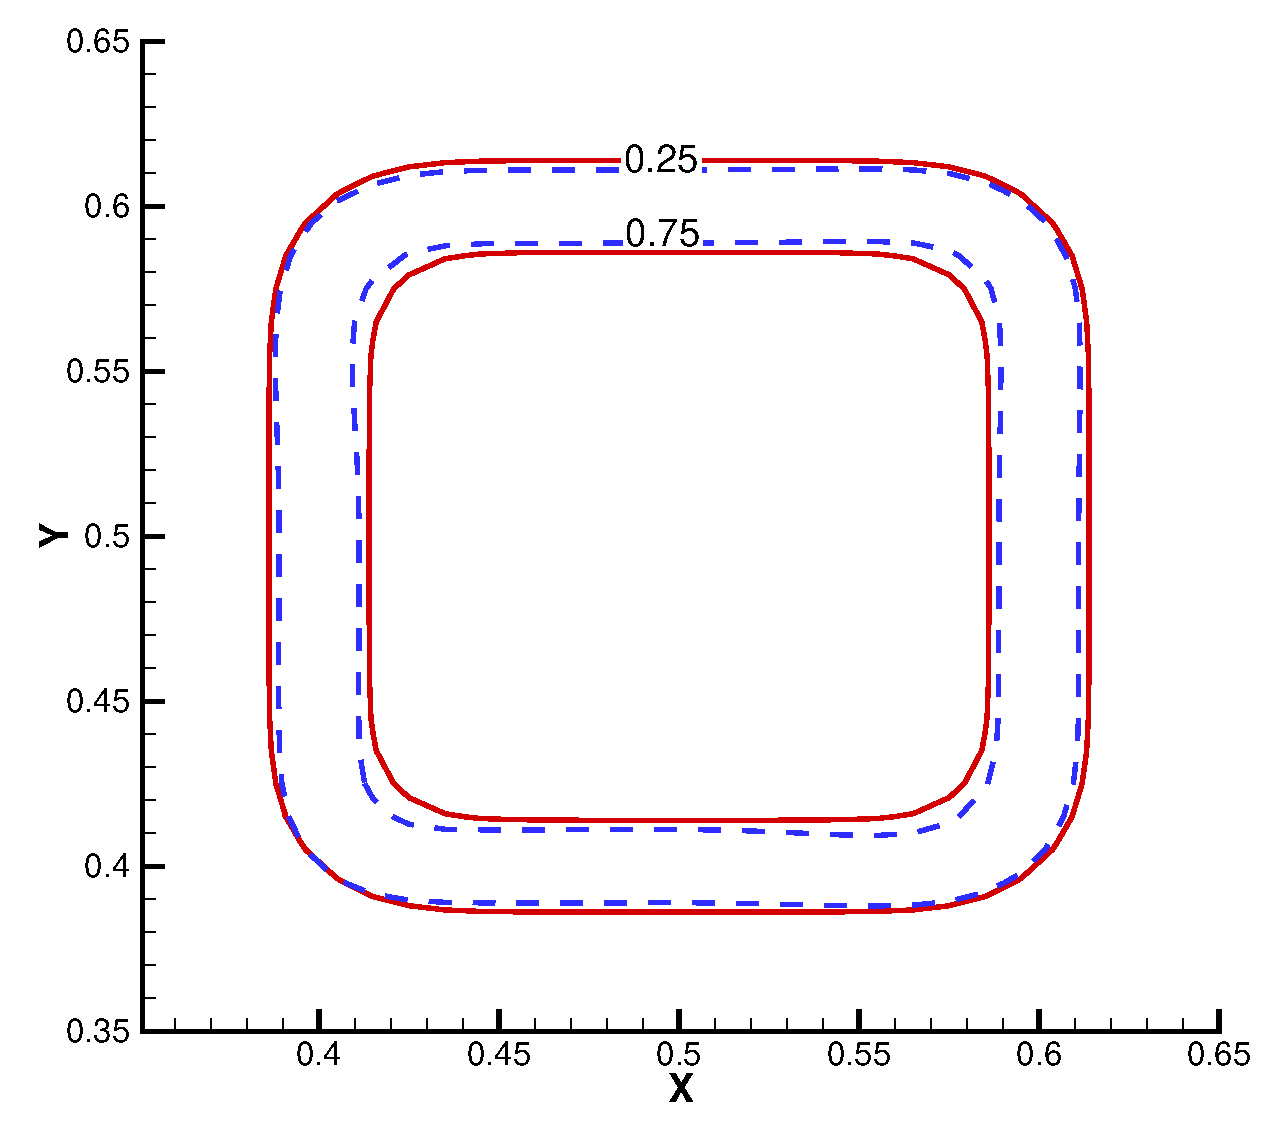
\includegraphics[width=0.45\textwidth]{figure/2D-sharp/large.eps}
%     }
%     \hfill
%     \subfloat[局部放大视图]{
%         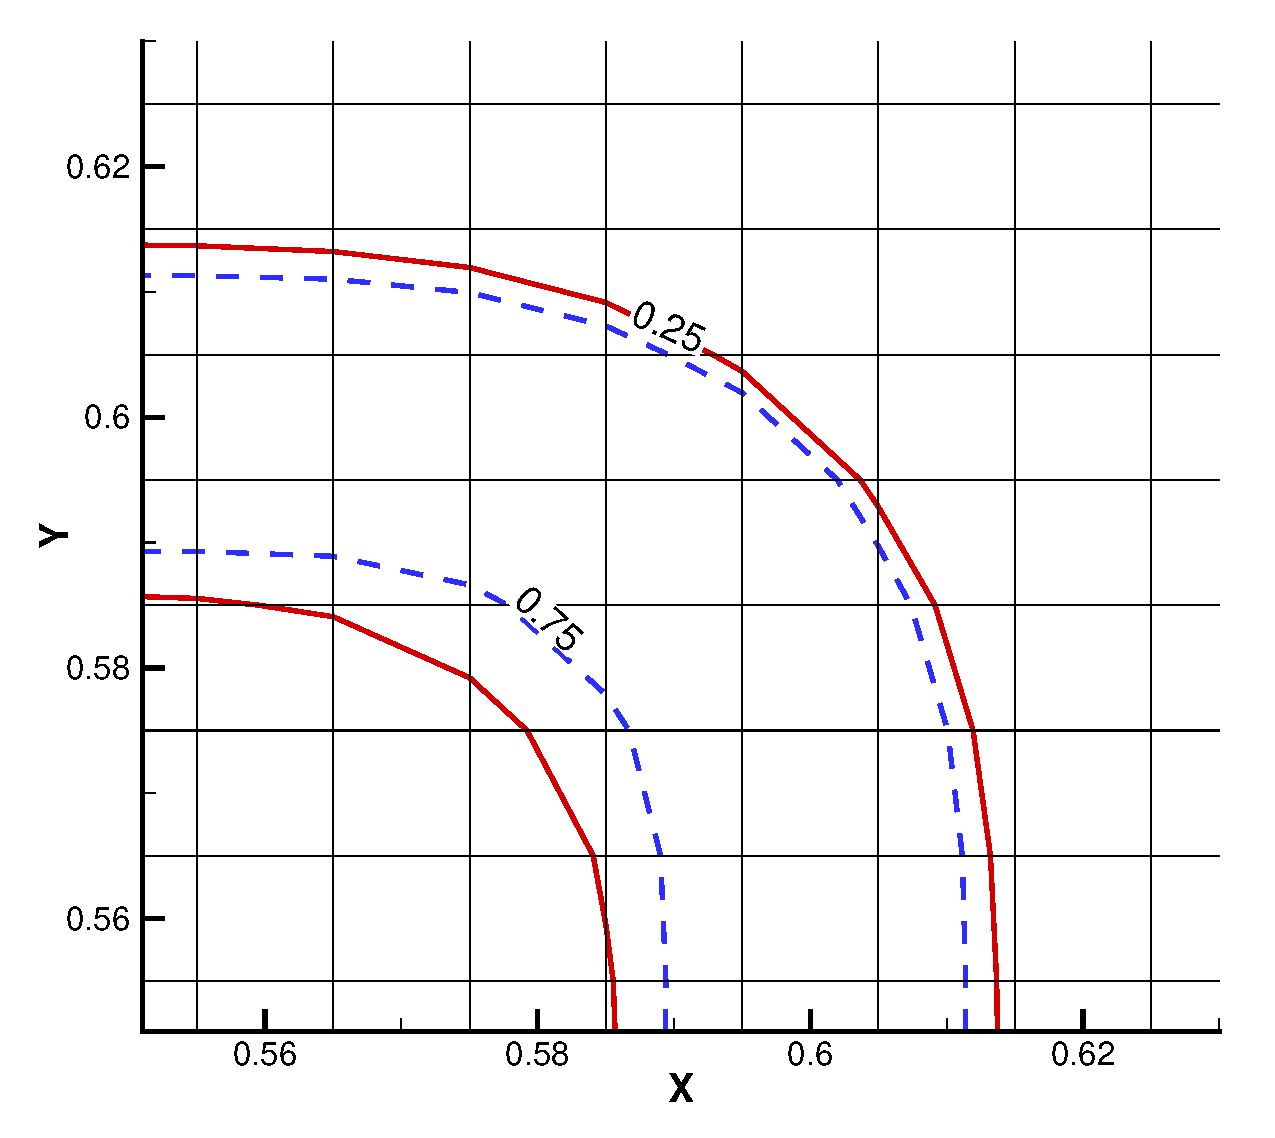
\includegraphics[width=0.45\textwidth]{figure/2D-sharp/small.eps}
%     }
%     \caption{二维锐利界面平流问题中体积分数分布（蓝色虚线：WENO-JS；红色实线：WENO-EXP）。}
%     \label{fig:2Dinterface1}
% \end{figure}
% 为定量刻画界面宽度，引入如下定义：
% \begin{equation}
%   n_{\text{thickness}} = 1 / \max_{i,j}\left(\left|\overline{(z_1)}_{i,j} - \overline{(z_1)}_{i+1,j}\right|, \left|\overline{(z_1)}_{i,j} - \overline{(z_1)}_{i,j+1}\right| \right).
% \end{equation}
% 显然，$n_{\text{thickness}}$ 的值越小，对应的界面越锐利。\autoref{fig:2Dinterface2} 展示了 WENOJS 格式与 WENO-EXP 格式计算所得 $n_{\text{thickness}}$ 的时间演化曲线。结果表明，WENO-EXP 格式所得 $n_{\text{thickness}}$ 的值始终低于 WENOJS 格式，且两者之间的差距随时间推移逐渐增大。具体而言，在 $t = 1$ 时刻，WENO-EXP 格式的 $n_{\text{thickness}}$ 较 WENOJS 格式降低了约 $25\%$。
% \begin{figure}[htbp]
%     \centering
%     \subfloat[$100\times 100$ 网格]{
%         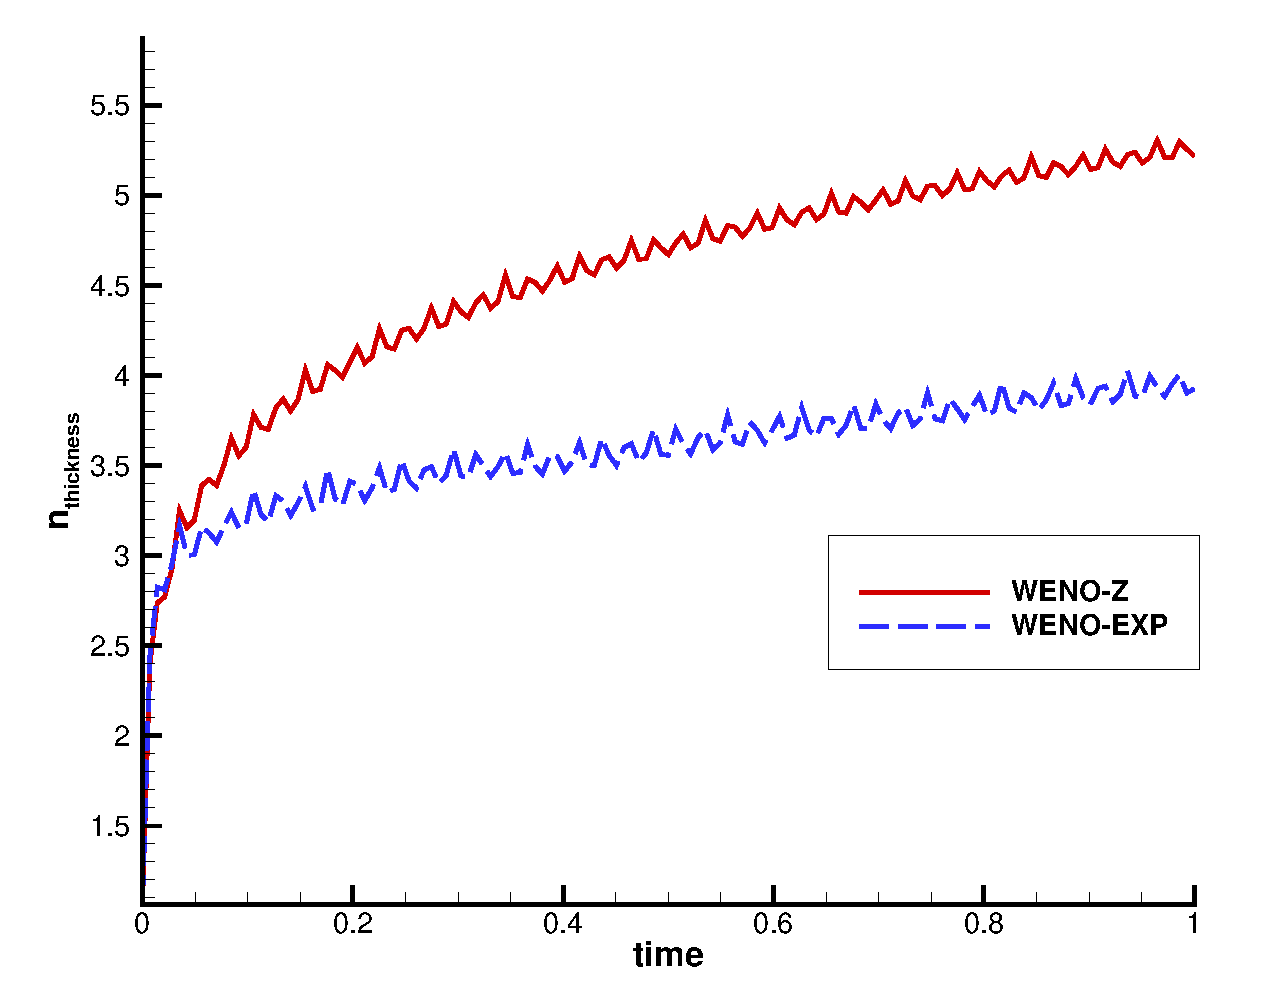
\includegraphics[width=0.45\textwidth]{figure/2D-sharp/100-thinckness.eps}
%     }
%     \hfill
%     \subfloat[$200\times 200$ 网格]{
%         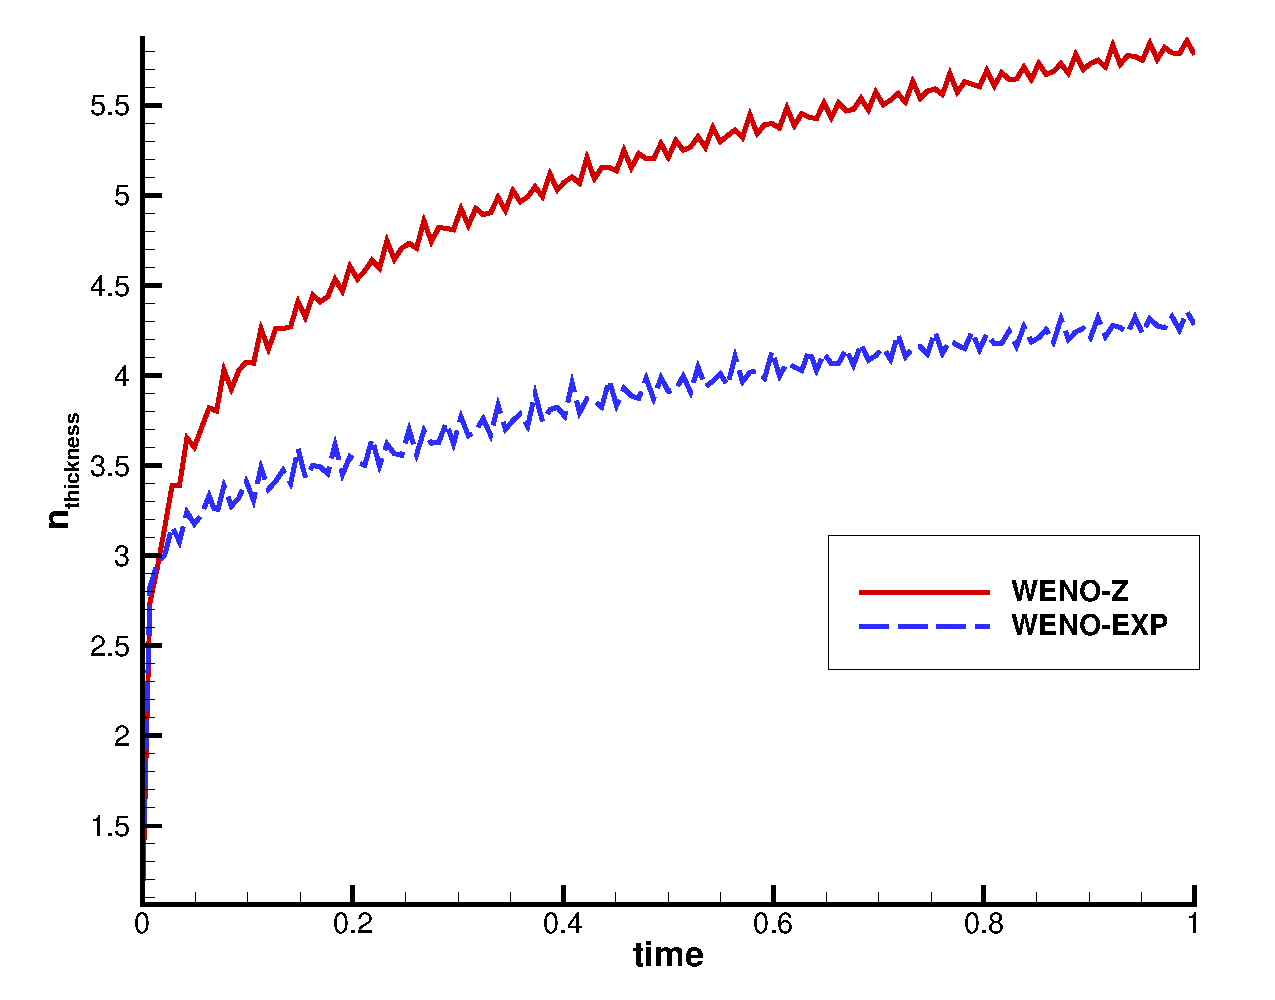
\includegraphics[width=0.45\textwidth]{figure/2D-sharp/200-thinckness.eps}
%     }
%     \\
%     \caption{二维锐利界面平流问题界面厚度指标 $n_{\text{thickness}}$ 的时间演化。}
%     \label{fig:2Dinterface2}
% \end{figure}


% \autoref{fig:2DOscillation} 展示了采用不同重构变量的 WENO-EXP 格式所得速度与压力振荡情况。结果表明，基于 prim2 重构的 WENO-EXP 格式在维持近似均匀压力场与速度场方面，相较于基于 prim1 重构的 WENO-EXP 格式具有更优越的性能。该结论与一维算例所得结论一致。

% \begin{figure}[htbp]
%     \centering
%     \subfloat[速度振荡]{
%         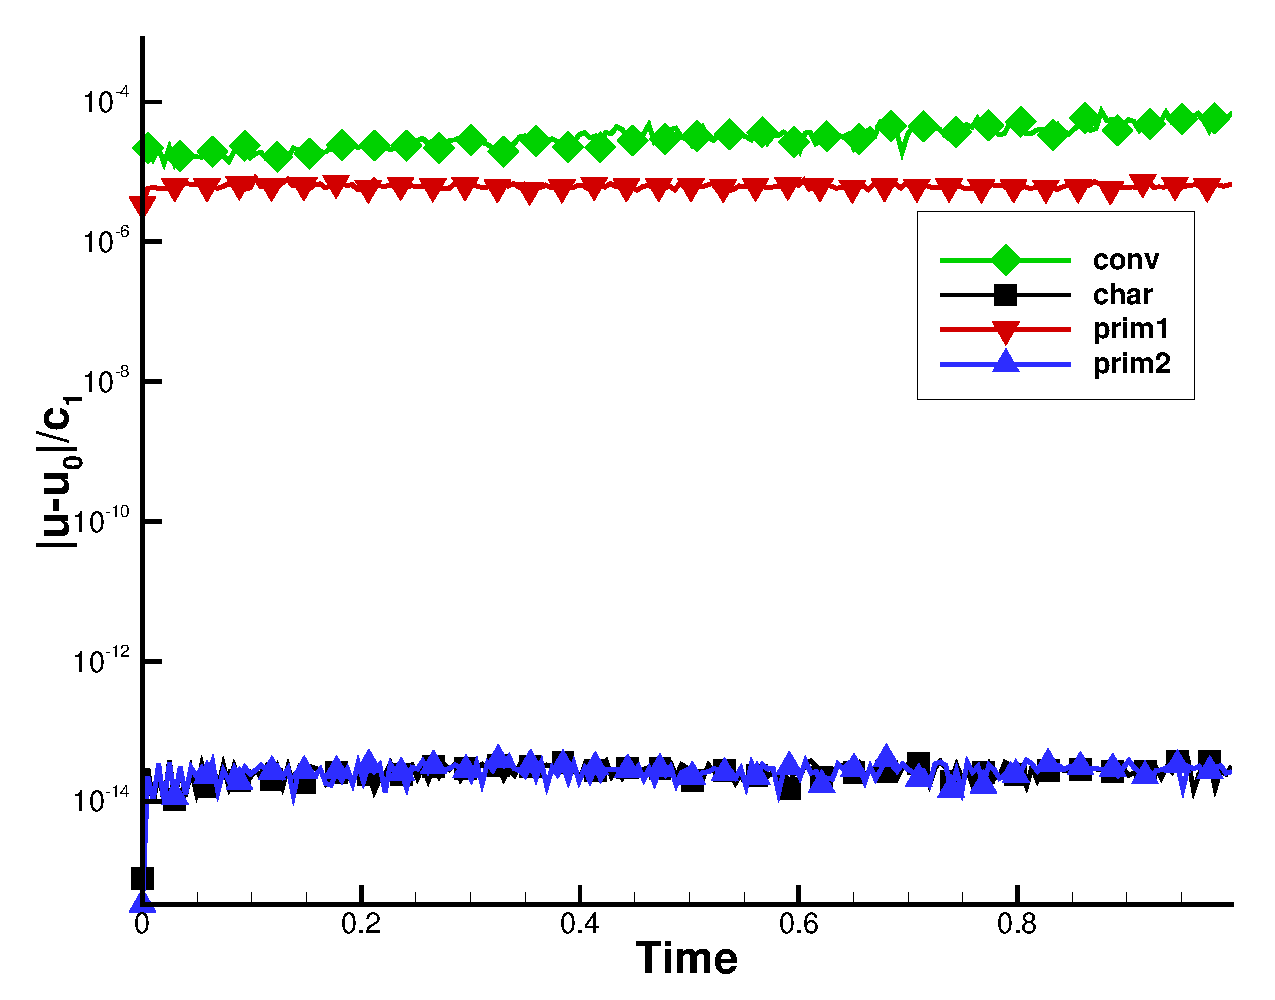
\includegraphics[width=0.45\textwidth]{figure/2D-sharp/speed.eps}
%     }
%     \hfill
%     \subfloat[压力振荡]{
%         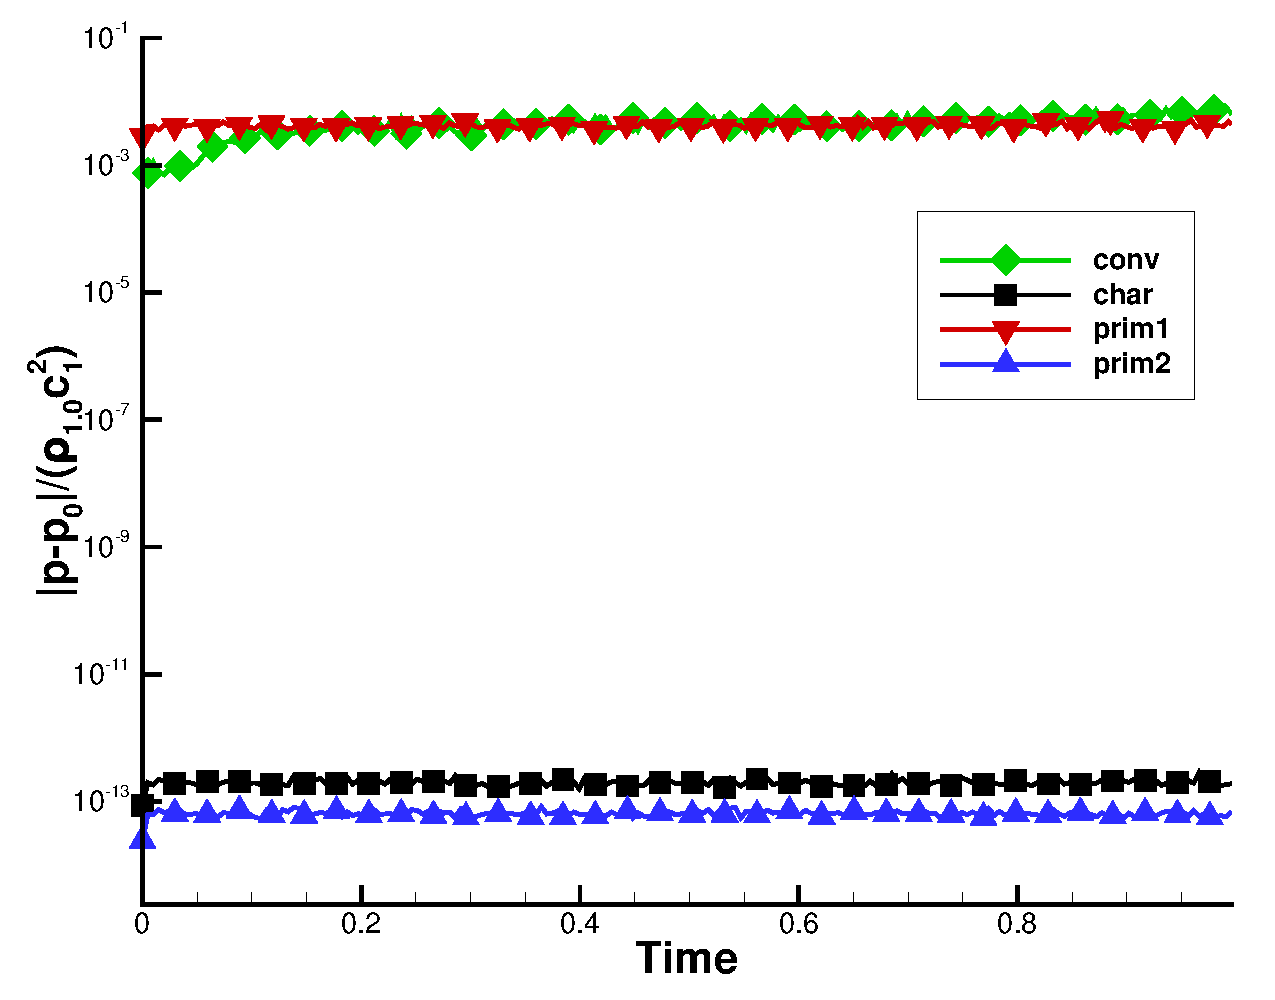
\includegraphics[width=0.45\textwidth]{figure/2D-sharp/pressure.eps}
%     }
%     \caption{采用不同重构变量的WENO-EXP格式对二维清晰界面平流问题的数值振荡计算结果。}
%     \label{fig:2DOscillation}
% \end{figure}

% \autoref{tab:time_cost} 给出了采用不同重构变量的 WENO-EXP 格式之间的计算效率对比。以守恒变量重构（conv）格式为基准，该格式所需计算时间最短。基于特征变量的重构格式由于引入了额外的特征分解过程，计算开销相应增加约 $30\%$。值得注意的是，基于原始变量的两种重构格式（prim1 与 prim2）均保持了接近最优的计算效率。上述结果表明，所提格式在计算效率方面具有显著优势。

% \begin{table}[htbp]
%   \centering
%   \caption{二维锐利界面对流问题的 CPU 计算时间。}
%   \begin{tabular}{lcccc}
%     \toprule
%     指标                & conv  & char  & prim1 & prim2 \\
%     \midrule
%     CPU 时间 (min)      & 35.81 & 46.34 & 37.56 & 36.93 \\
%     相对计算开销        & 1.00  & 1.29  & 1.05  & 1.03  \\
%     \bottomrule
%   \end{tabular}
%   \label{tab:time_cost}
% \end{table}

% % \subsection{Zalesak 刚性旋转问题}

% % 本算例通过 Zalesak 凹齿圆盘在匀角速度场中的刚性旋转问题~\cite{}
% % 进一步验证所提格式的界面捕获精度。圆盘圆心位于
% % $(0.75~\mathrm{m},\, 0.5~\mathrm{m})$，
% % 直径为 $0.3~\mathrm{m}$，凹槽宽度为 $0.05~\mathrm{m}$，
% % 与圆周间隙为 $0.05~\mathrm{m}$，盘内区域为液相。
% % 旋转速度场由下式给定：
% % \begin{equation}
% %     u = -\omega(0.5 - y)~\mathrm{m/s}, \qquad v = -\omega(x - 0.5)~\mathrm{m/s},
% % \end{equation}
% % 其中角速度 $\omega = \pi~\mathrm{rad/s}$，对应旋转周期 $T = 2~\mathrm{s}$。
% % 分别采用 $50\times 50$、$100\times 100$ 和 $200\times 200$ 三种网格进行计算，
% % CFL 数取 $1.0$，共计算 $10000$ 个时间步。

% % 图~X 给出了旋转一圈后各格式所得体积分数分布与初始形状的对比。
% % 结果表明，随着网格加密，数值结果与初始圆盘形状的吻合程度不断提高，
% % 凹槽形状和圆弧轮廓均得到较好保持。在相同网格下，
% % WENO-EXP-II 格式相较于 WENO-JS 格式产生更少的界面弥散，
% % 界面轮廓更为锐利清晰。


% \subsection{低幅值驻波问题}
% 本算例考虑低幅值驻波问题~\cite{Sussman2007,Frandsen2003}，用于验证所提格式在自由液面水动力学问题中的性能。初始时刻，空气与水在重力作用下静止于正方形容器 $\Omega = [0, 0.5~\mathrm{m}]^2$ 内，容器四周为自由滑移固壁边界，初始构型如~\autoref{fig:low-amplitude-standing-wave} 所示。物理参数设置为：重力加速度 $\bm{g} = (0, -2\pi)^\top~\mathrm{m/s^2}$，密度比 $\rho_{1,0}/\rho_{2,0} = 1000$，两相声速均取 $c_1 = c_2 = 100~\mathrm{m/s}$，背景压力 $p_0 = 10{,}000~\mathrm{Pa}$。偏离平衡位置的气-水界面在重力作用下产生周期性振荡，液面形态随时间往复变化，形成驻波。

% \begin{figure}[!htbp]
%     \centering
%     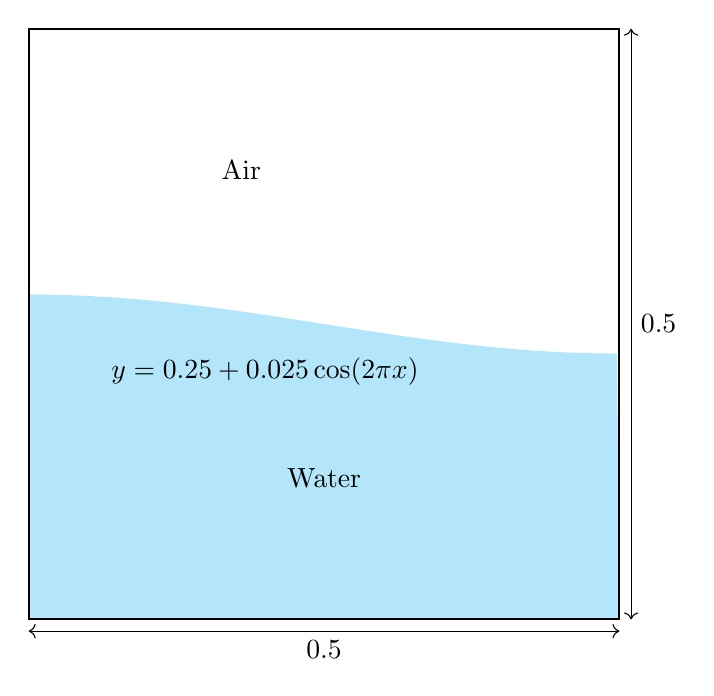
\begin{tikzpicture}[scale=15]


% Water region (blue fill, below interface)
\fill[cyan!30, domain=0:0.5, samples=200]
(0,0)
-- plot (\x, {0.25 + 0.025*cos(360*\x)})
-- (0.5,0)
-- cycle;

% Phase labels
\node at (0.18,0.38) {Air};
\node at (0.25,0.12) {Water};

% Gravity vector
% \draw[->, thick] (0.3,0.35) -- (0.3,0.25)
% node[midway, right] {$\boldsymbol{g}=(0,-2\pi)^{\mathrm{T}}$};

% ---- Dimension annotations ----
% Horizontal length 0.5
\draw[<->] (0,-0.01) -- (0.5,-0.01)
node[midway, below] {$0.5$};

% Vertical length 0.5
\draw[<->] (0.51,0) -- (0.51,0.5)
node[midway, right] {$0.5$};

% ---- Interface annotation ----
\node at (0.2,0.21)
{$y=0.25+0.025\cos(2\pi x)$};

% Domain boundary
\draw[thick] (0,0) rectangle (0.5,0.5);


\end{tikzpicture}

%     \caption{低幅值驻波问题初始构型示意图。}
%     \label{fig:low-amplitude-standing-wave}
% \end{figure}

% 图~\autoref{fig:low-amplitude-standing-wave-exp} 展示了采用 WENO-EXP 格式在 $128 \times 128$ 网格下计算所得体积分数 $z_1$ 分布随时间的演化结果。由图可见，界面始终保持清晰，无明显数值耗散引起的界面弥散现象，液面振荡过程中两相分布对称性良好，表明所提格式在大密度比自由液面问题中具有较强的界面捕捉能力和长时间计算的稳定性。

% \begin{figure}[!htbp]
%     \centering
%     \begin{subfigure}[t]{0.18\linewidth}
%         \centering
%         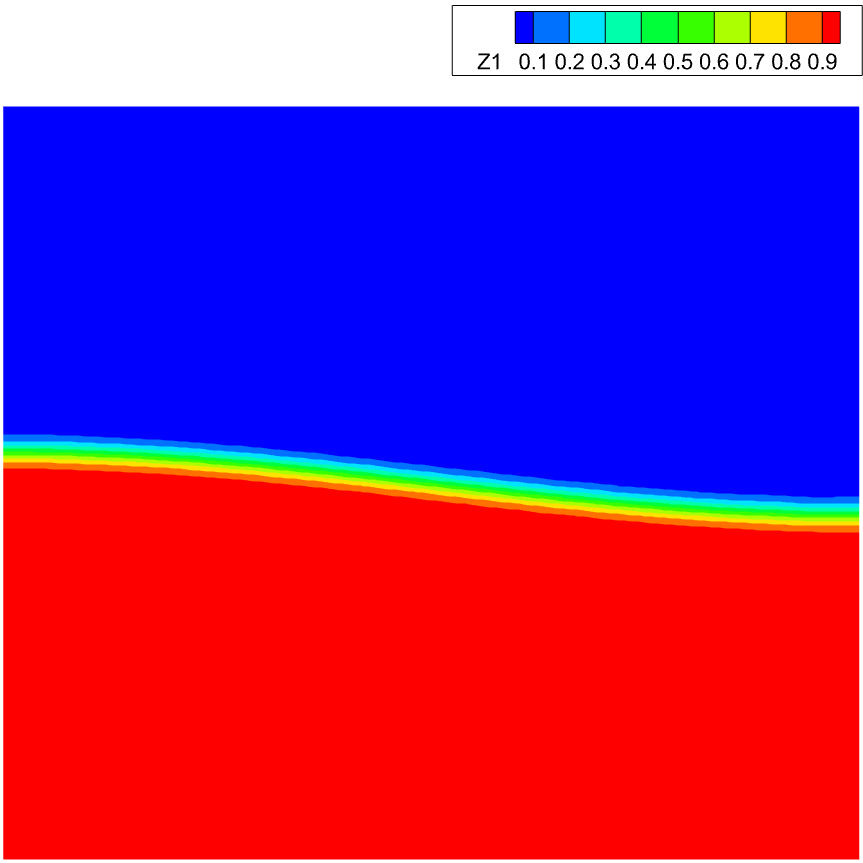
\includegraphics[width=\linewidth]{figure/problem-low-amplitude-standing-wave/z1/wenojs-1.png}
%     \end{subfigure}
%     \begin{subfigure}[t]{0.18\linewidth}
%         \centering
%         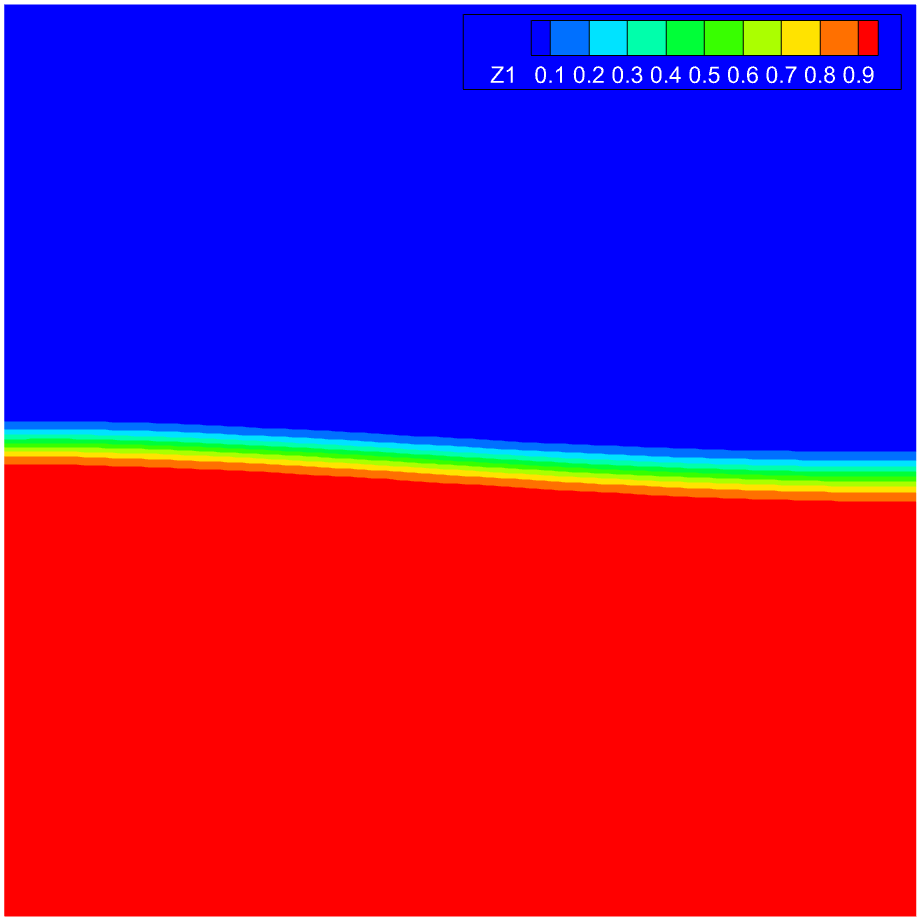
\includegraphics[width=\linewidth]{figure/problem-low-amplitude-standing-wave/z1/wenojs-2.png}
%     \end{subfigure}
%     \begin{subfigure}[t]{0.18\linewidth}
%         \centering
%         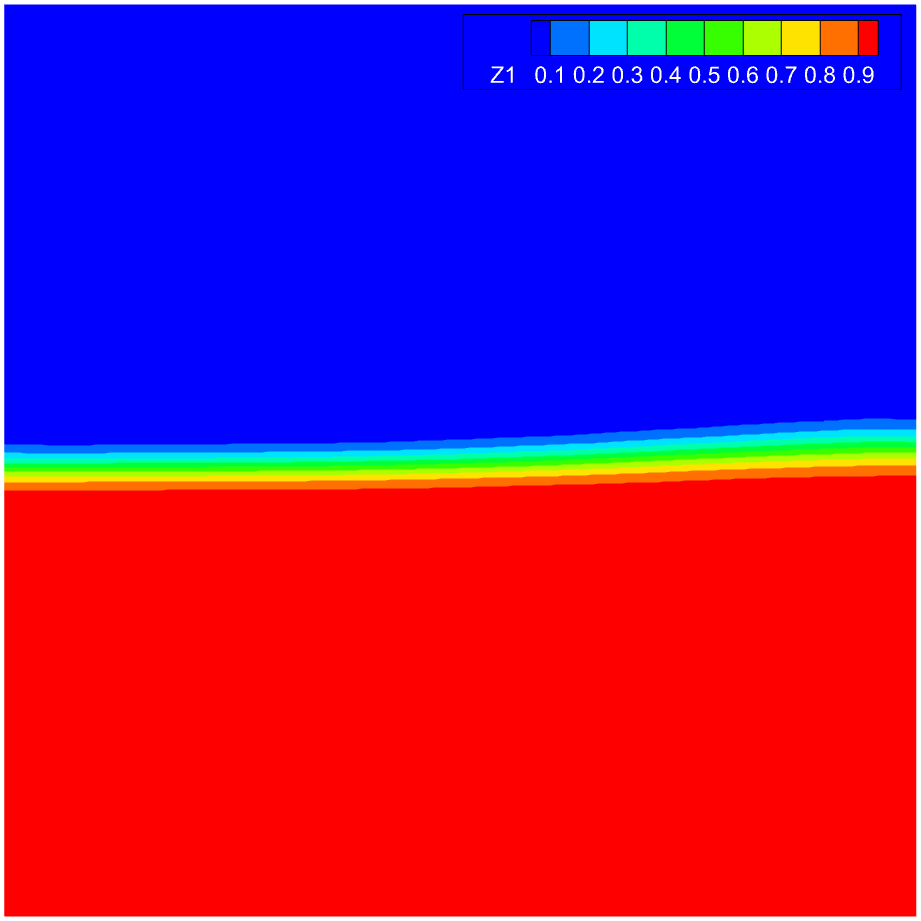
\includegraphics[width=\linewidth]{figure/problem-low-amplitude-standing-wave/z1/wenojs-3.png}
%     \end{subfigure}
%     \begin{subfigure}[t]{0.18\linewidth}
%         \centering
%         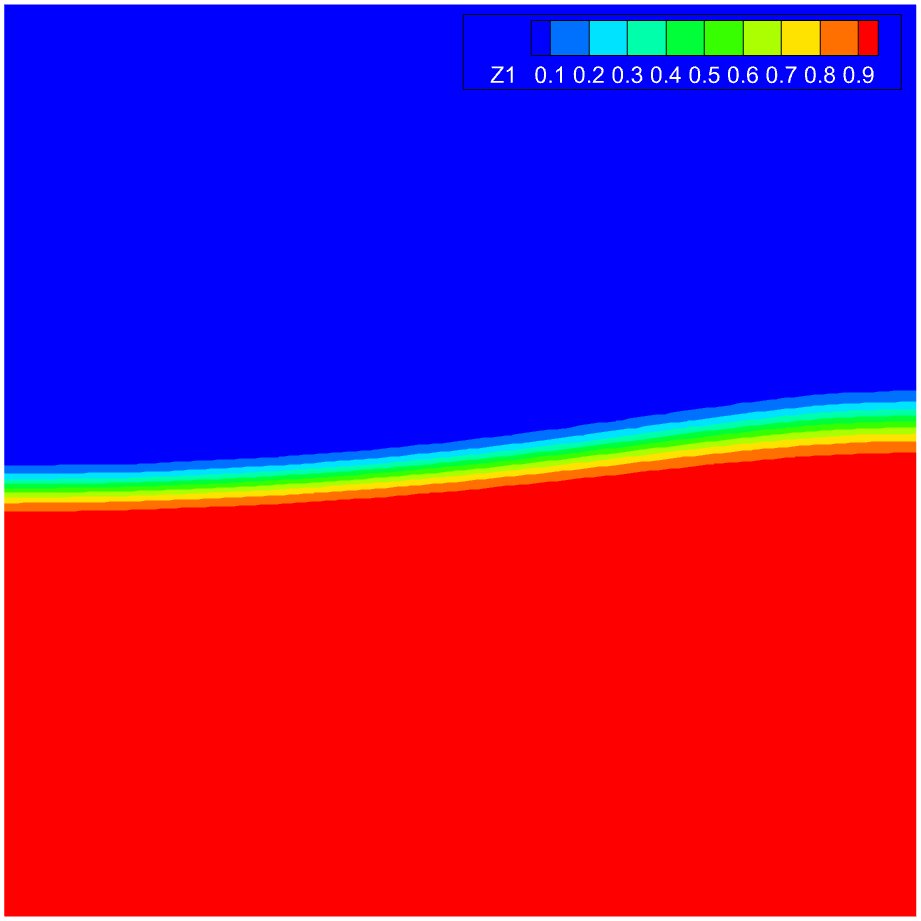
\includegraphics[width=\linewidth]{figure/problem-low-amplitude-standing-wave/z1/wenojs-4.png}
%     \end{subfigure}
%     \begin{subfigure}[t]{0.18\linewidth}
%         \centering
%         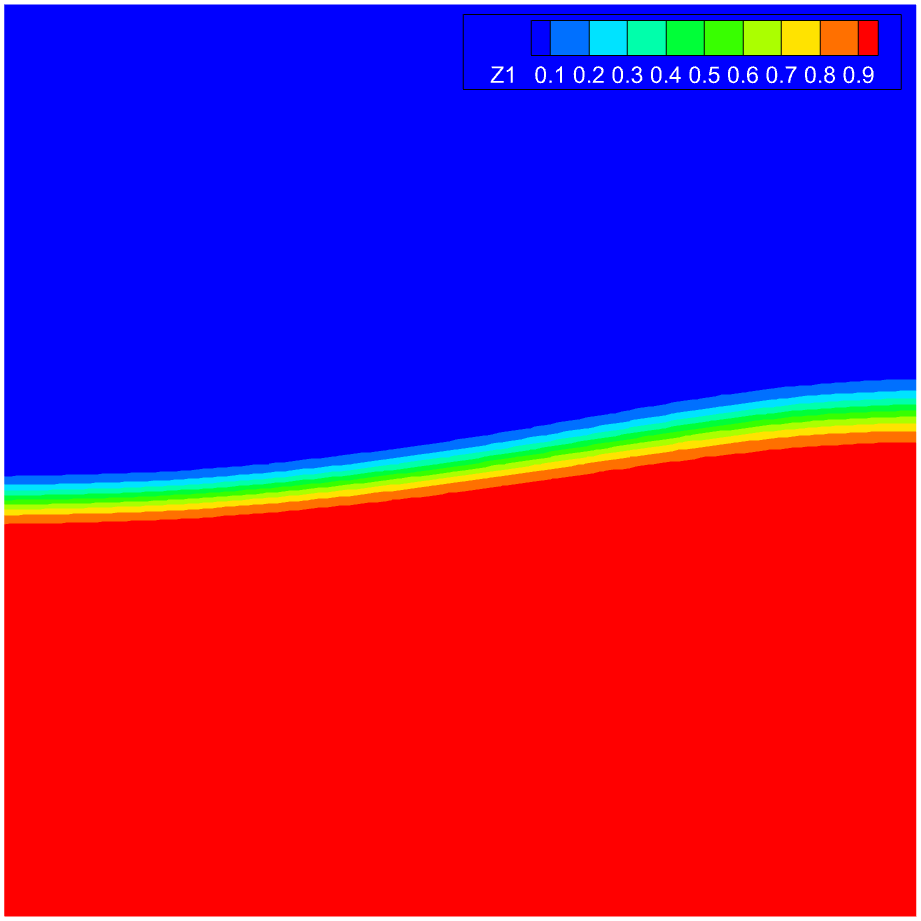
\includegraphics[width=\linewidth]{figure/problem-low-amplitude-standing-wave/z1/wenojs-5.png}
%     \end{subfigure}\\
%     \begin{subfigure}[t]{0.18\linewidth}
%         \centering
%         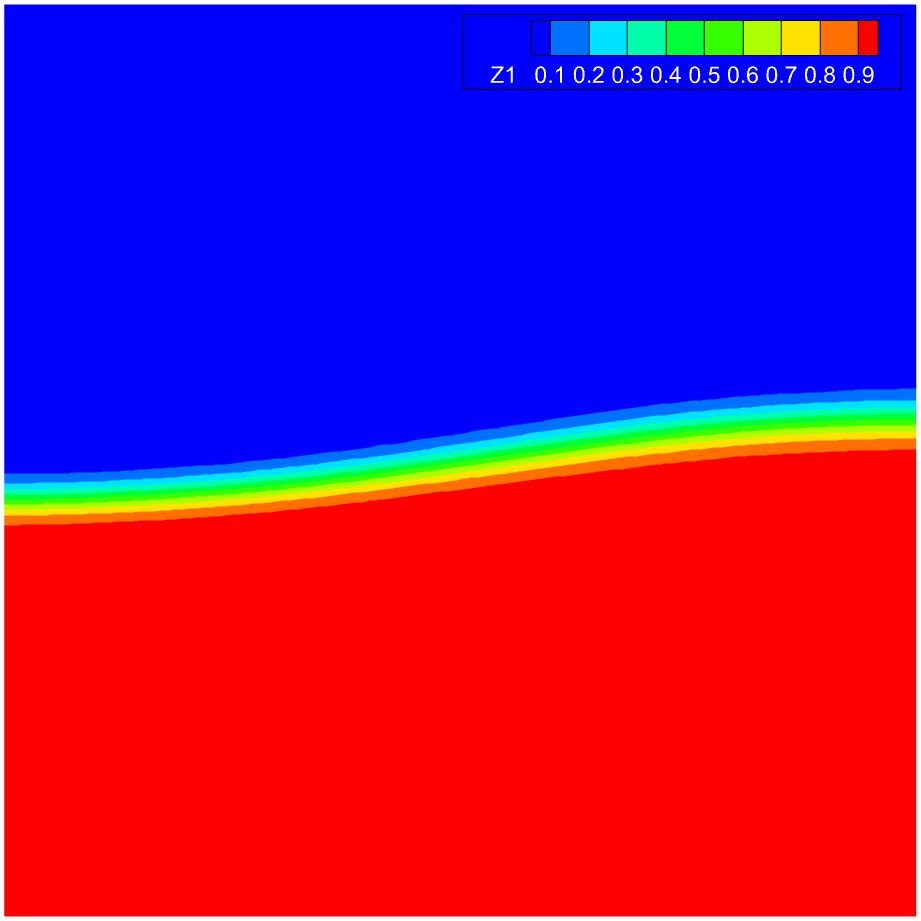
\includegraphics[width=\linewidth]{figure/problem-low-amplitude-standing-wave/z1/wenojs-6.png}
%     \end{subfigure}
%     \begin{subfigure}[t]{0.18\linewidth}
%         \centering
%         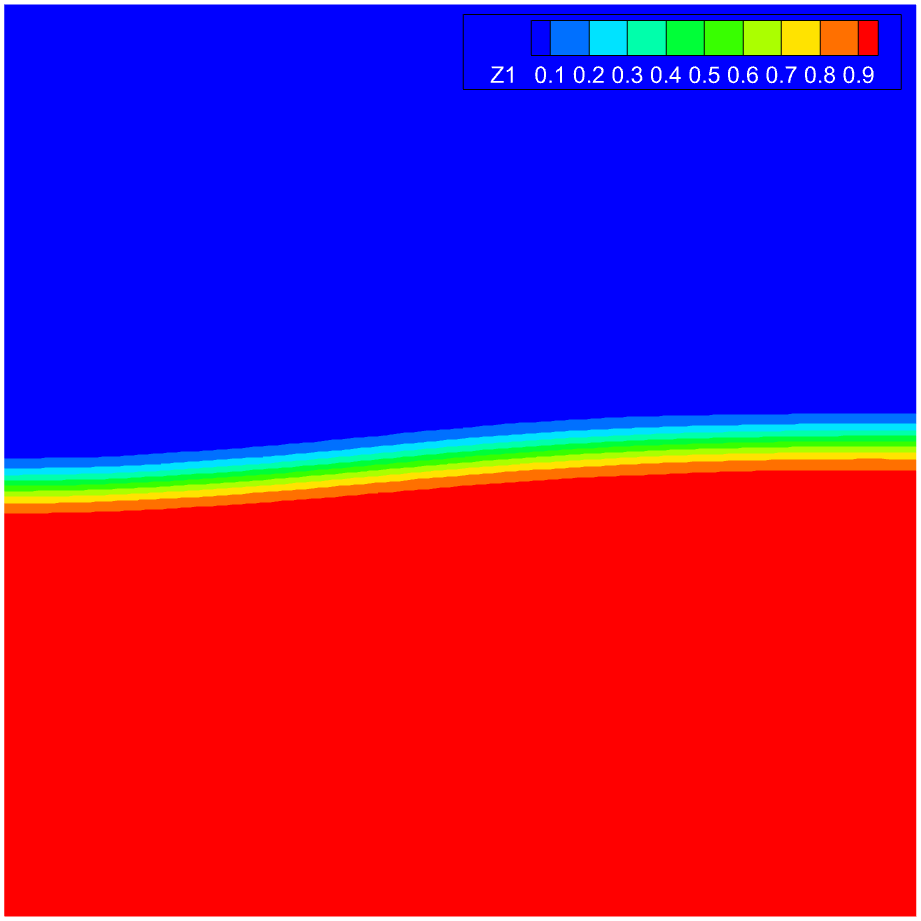
\includegraphics[width=\linewidth]{figure/problem-low-amplitude-standing-wave/z1/wenojs-7.png}
%     \end{subfigure}
%     \begin{subfigure}[t]{0.18\linewidth}
%         \centering
%         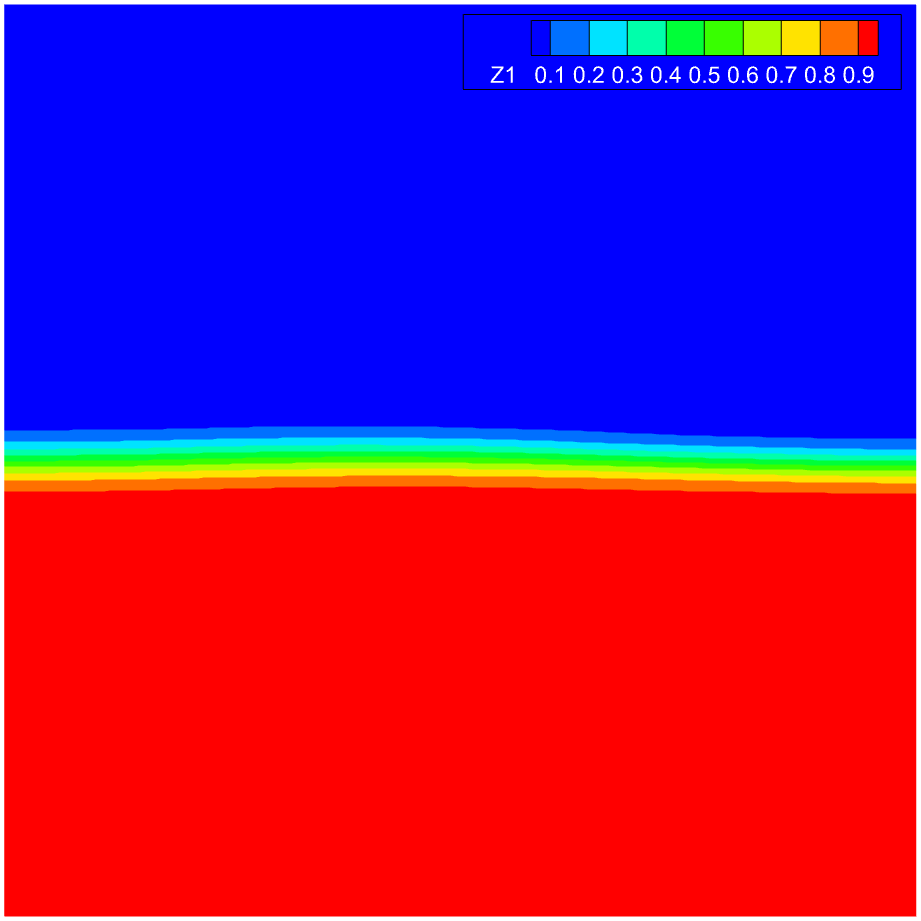
\includegraphics[width=\linewidth]{figure/problem-low-amplitude-standing-wave/z1/wenojs-8.png}
%     \end{subfigure}
%     \begin{subfigure}[t]{0.18\linewidth}
%         \centering
%         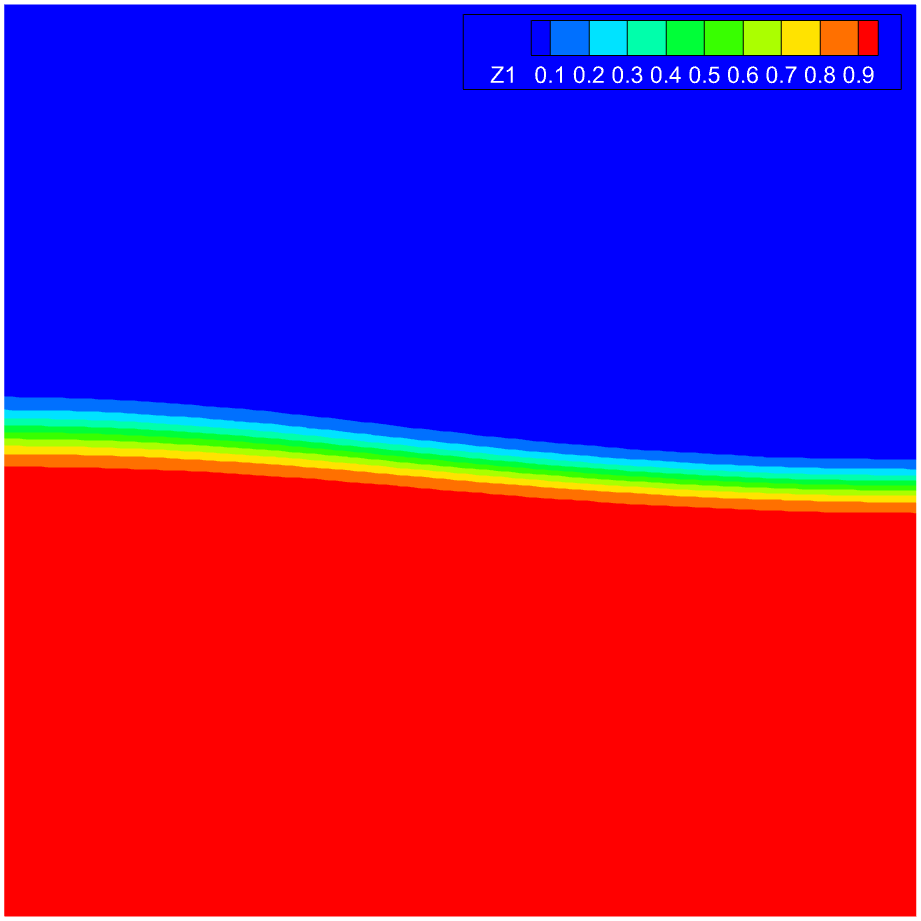
\includegraphics[width=\linewidth]{figure/problem-low-amplitude-standing-wave/z1/wenojs-9.png}
%     \end{subfigure}
%     \begin{subfigure}[t]{0.18\linewidth}
%         \centering
%         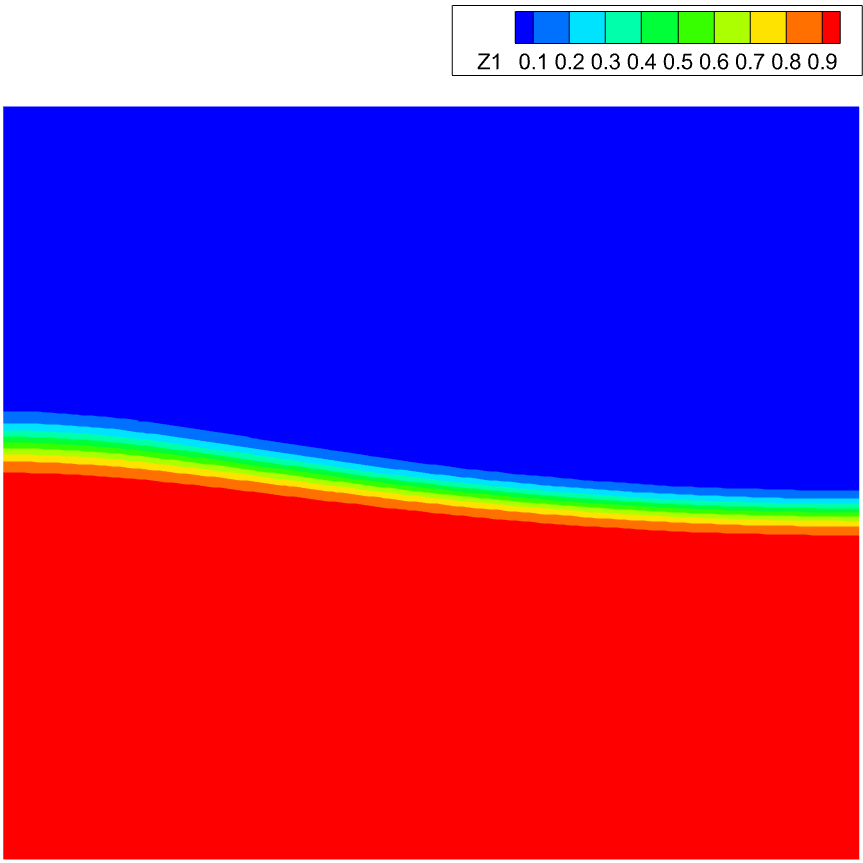
\includegraphics[width=\linewidth]{figure/problem-low-amplitude-standing-wave/z1/wenojs-10.png}
%     \end{subfigure}\\
%     \caption{体积分数 $z_1$ 随时间演化，WENO-EXP 格式，$128\times 128$ 网格。}
%     \label{fig:low-amplitude-standing-wave-exp}
% \end{figure}

% 基于二阶小扰动理论~\cite{Frandsen2003}，低幅值自由液面运动的理论振荡周期为 $T \approx 1.04~\mathrm{s}$。表~\autoref{tab:low-amplitude-standing-wave-period} 列出了 WENO-JS 与 WENO-EXP 格式在不同网格分辨率下数值计算所得的振荡周期。结果表明，两种格式在各网格层次上均与理论值吻合良好，且随着网格加密，所得周期逐渐收敛至参考值。WENO-EXP 格式与 WENO-JS 格式的计算结果相近，说明所提格式在该问题上具有与经典格式相当的精度表现。

% \begin{table}[!htbp]
%     \centering
%     \caption{低幅值驻波问题振荡周期（单位：s）。}
%     \label{tab:low-amplitude-standing-wave-period}
%     \begin{tabular}{lccc}
%         \toprule
%         网格 & $32 \times 32$ & $64 \times 64$ & $128 \times 128$ \\
%         \midrule
%         WENO-JS  & 1.00 & 1.03 & 1.05 \\
%         WENO-EXP & 1.07 & 1.06 & 1.05 \\
%         \bottomrule
%     \end{tabular}
% \end{table}

% % 本算例考虑低幅值驻波问题~\cite{Sussman2007,Frandsen2003}，用于验证所提格式在自由液面水动力学问题中的性能。初始时刻，空气与水在重力作用下静止于正方形容器$\Omega = [0, 0.5~\mathrm{m}]^2$ 内，容器四周为自由滑移固壁边界，初始构型如~\autoref{fig:low-amplitude-standing-wave} 所示。
% % \begin{figure}[!htbp]
% %     \centering
% %     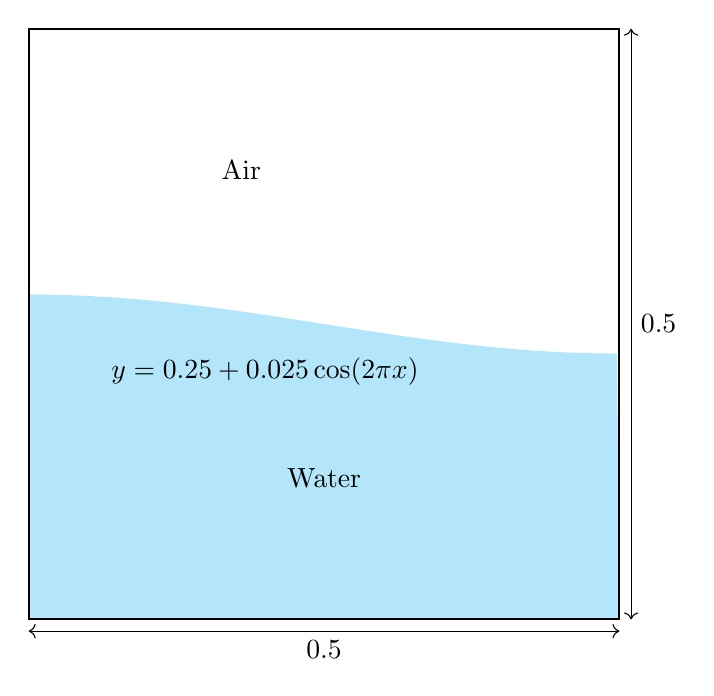
\begin{tikzpicture}[scale=15]


% Water region (blue fill, below interface)
\fill[cyan!30, domain=0:0.5, samples=200]
(0,0)
-- plot (\x, {0.25 + 0.025*cos(360*\x)})
-- (0.5,0)
-- cycle;

% Phase labels
\node at (0.18,0.38) {Air};
\node at (0.25,0.12) {Water};

% Gravity vector
% \draw[->, thick] (0.3,0.35) -- (0.3,0.25)
% node[midway, right] {$\boldsymbol{g}=(0,-2\pi)^{\mathrm{T}}$};

% ---- Dimension annotations ----
% Horizontal length 0.5
\draw[<->] (0,-0.01) -- (0.5,-0.01)
node[midway, below] {$0.5$};

% Vertical length 0.5
\draw[<->] (0.51,0) -- (0.51,0.5)
node[midway, right] {$0.5$};

% ---- Interface annotation ----
\node at (0.2,0.21)
{$y=0.25+0.025\cos(2\pi x)$};

% Domain boundary
\draw[thick] (0,0) rectangle (0.5,0.5);


\end{tikzpicture}

% %     \caption{低幅值驻波问题初始构型示意图。}
% %     \label{fig:low-amplitude-standing-wave}
% % \end{figure}

% % % 气-水初始界面由下式给出：
% % % \begin{equation}
% % %     y(x, 0) = 0.25 + 0.025\cos(2\pi x).
% % % \end{equation}
% % 物理参数设置为：重力加速度 $\bm{g} = (0, -2\pi)^\top~\mathrm{m/s^2}$，密度比 $\rho_{1,0}/\rho_{2,0} = 1000$，两相声速均取 $c_1 = c_2 = 100~\mathrm{m/s}$，背景压力 $p_0 = 10{,}000~\mathrm{Pa}$。偏离平衡位置的气-水界面在重力作用下产生周期性振荡，液面形态随时间往复变化，形成驻波。\autoref{fig:low-amplitude-standing-wave-exp} 展示了使用 WENOXP 格式计算所得体积分数分布随时间的演化结果。
% % \begin{figure}[!htbp]
% %     \centering
% %     \begin{subfigure}[t]{0.18\linewidth}
% %         \centering
% %         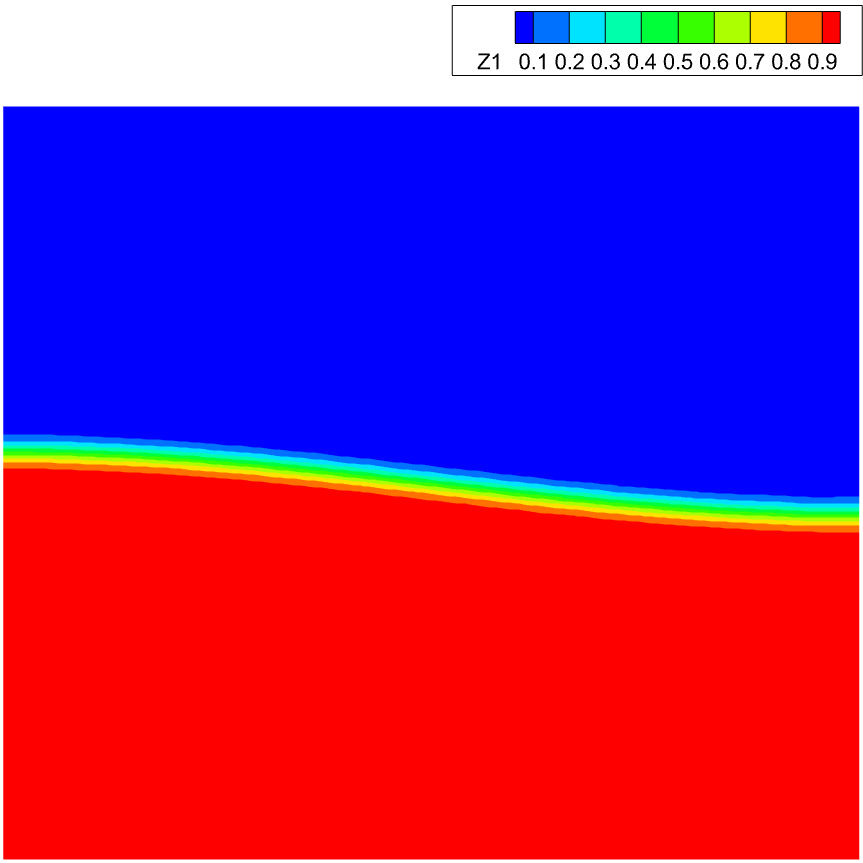
\includegraphics[width=\linewidth]{figure/problem-low-amplitude-standing-wave/z1/wenojs-1.png}
% %     \end{subfigure}
% %     \begin{subfigure}[t]{0.18\linewidth}
% %         \centering
% %         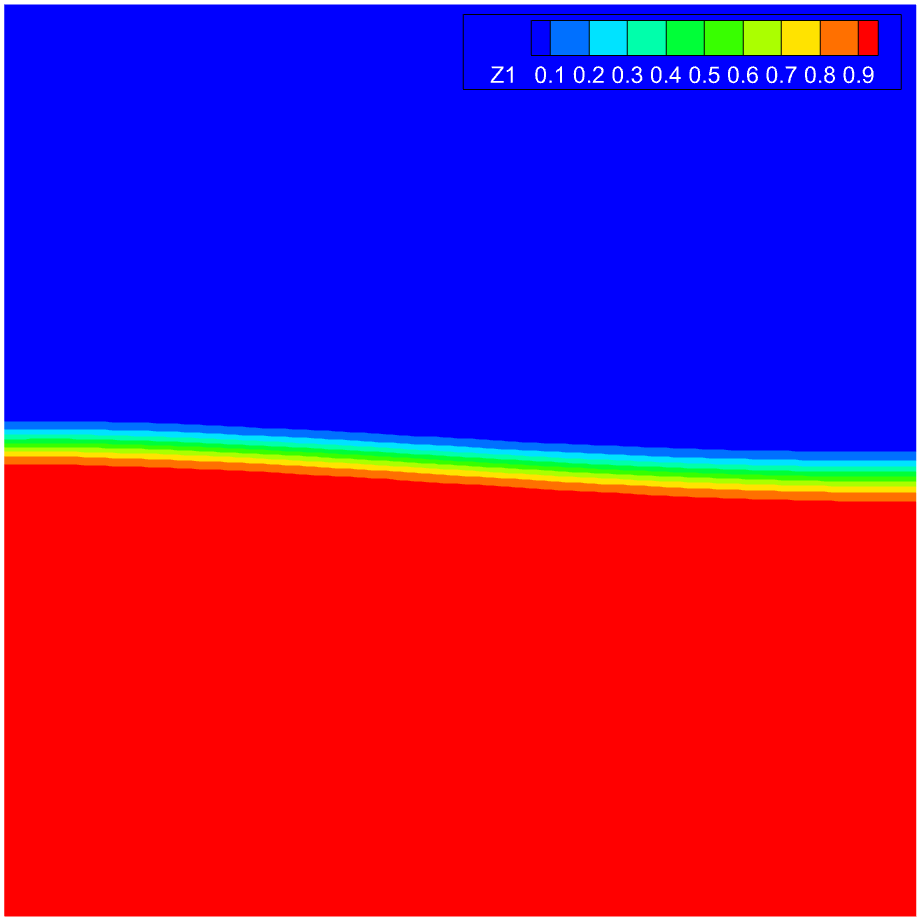
\includegraphics[width=\linewidth]{figure/problem-low-amplitude-standing-wave/z1/wenojs-2.png}
% %     \end{subfigure}
% %     \begin{subfigure}[t]{0.18\linewidth}
% %         \centering
% %         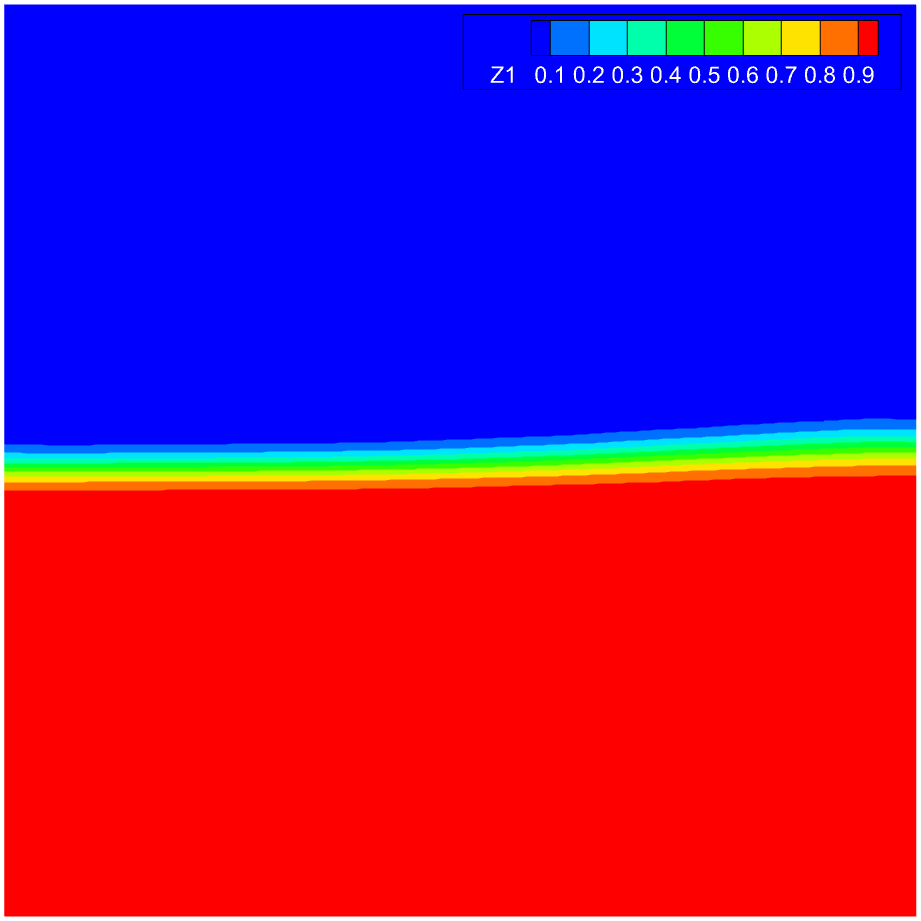
\includegraphics[width=\linewidth]{figure/problem-low-amplitude-standing-wave/z1/wenojs-3.png}
% %     \end{subfigure}
% %     \begin{subfigure}[t]{0.18\linewidth}
% %         \centering
% %         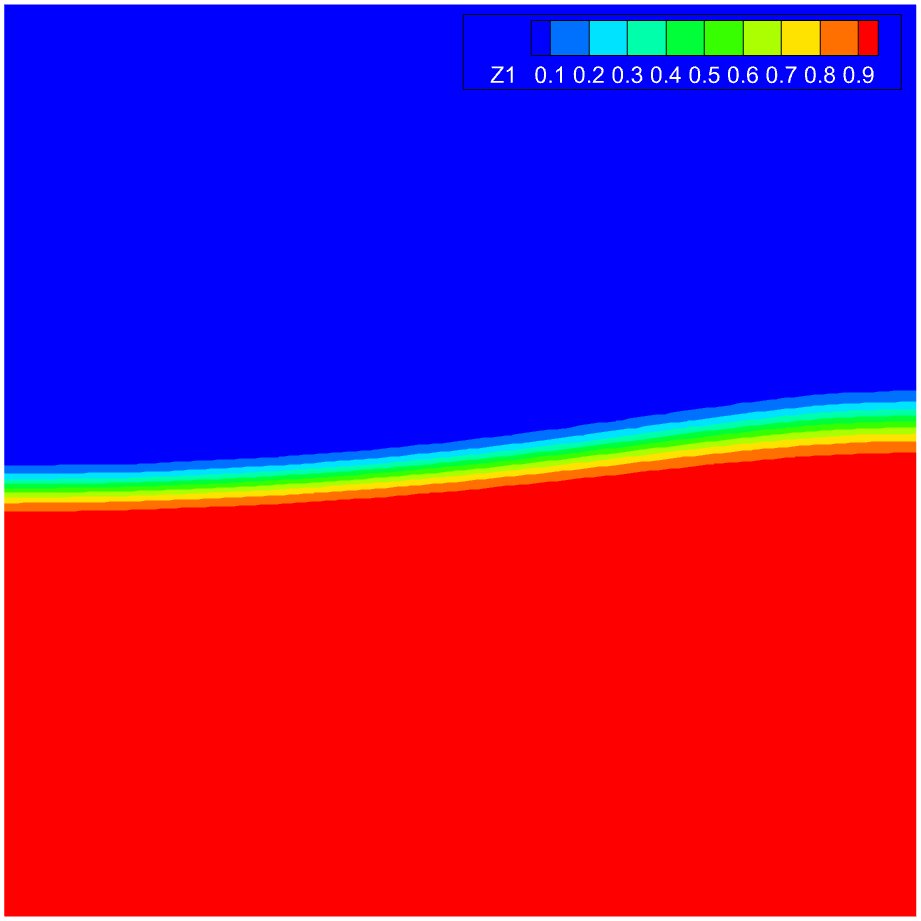
\includegraphics[width=\linewidth]{figure/problem-low-amplitude-standing-wave/z1/wenojs-4.png}
% %     \end{subfigure}
% %     \begin{subfigure}[t]{0.18\linewidth}
% %         \centering
% %         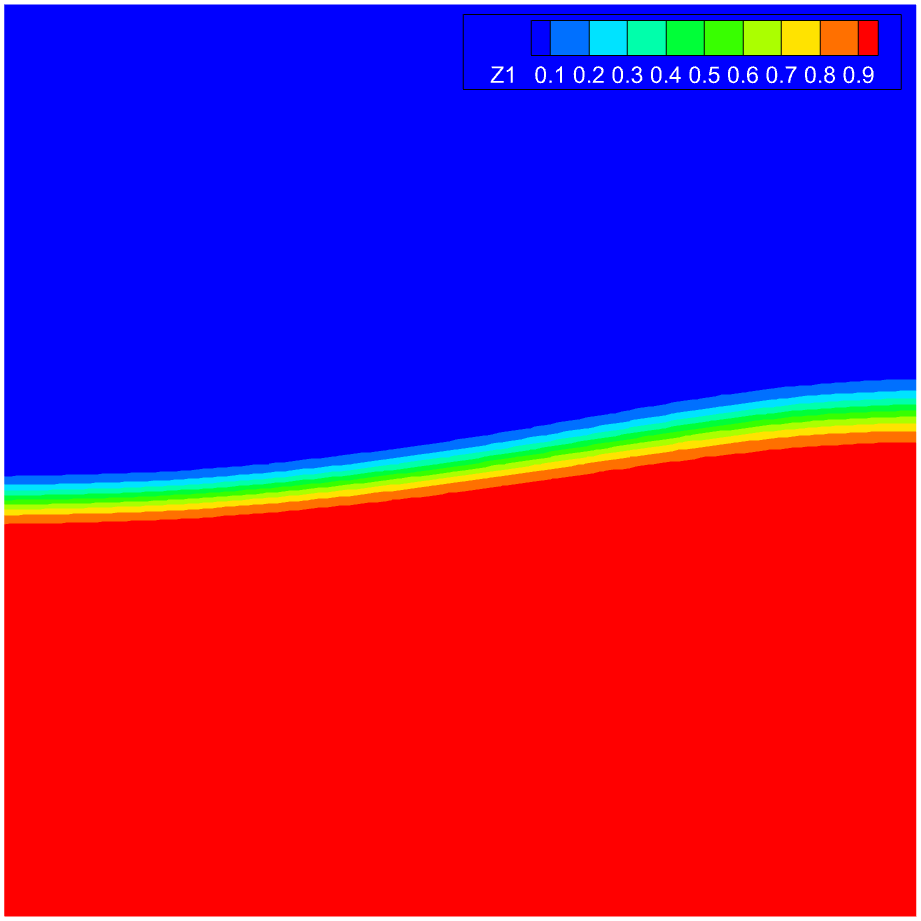
\includegraphics[width=\linewidth]{figure/problem-low-amplitude-standing-wave/z1/wenojs-5.png}
% %     \end{subfigure}\\ 
% %         \begin{subfigure}[t]{0.18\linewidth}
% %         \centering
% %         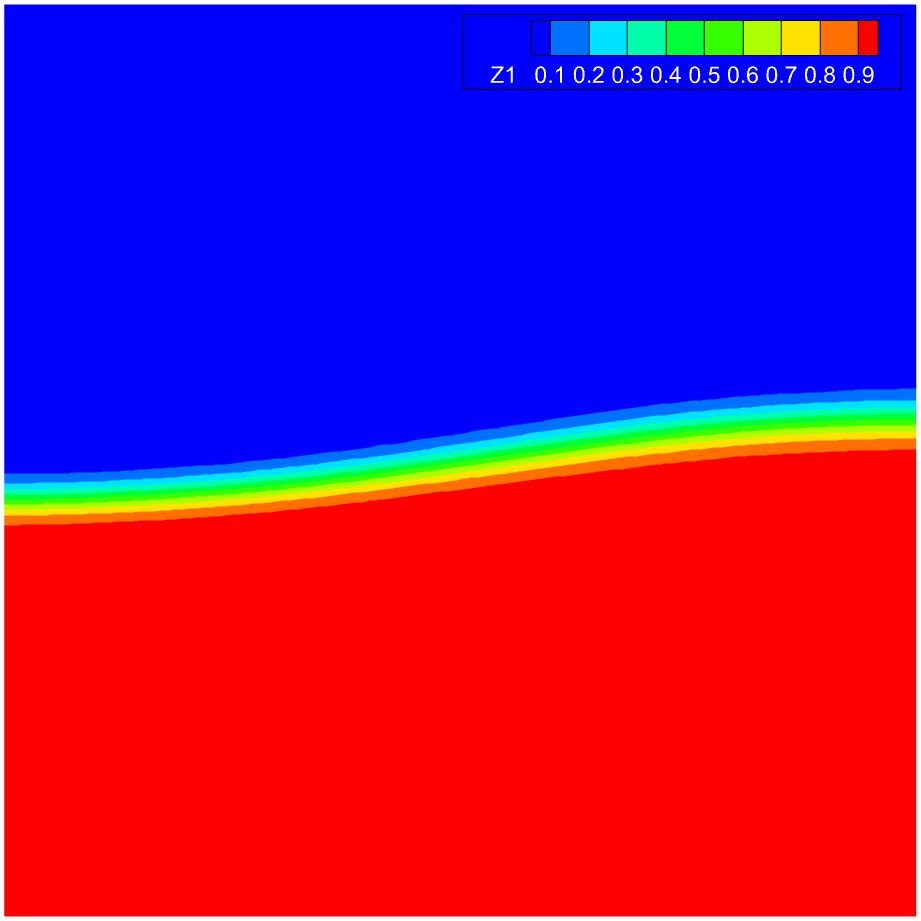
\includegraphics[width=\linewidth]{figure/problem-low-amplitude-standing-wave/z1/wenojs-6.png}
% %     \end{subfigure}
% %     \begin{subfigure}[t]{0.18\linewidth}
% %         \centering
% %         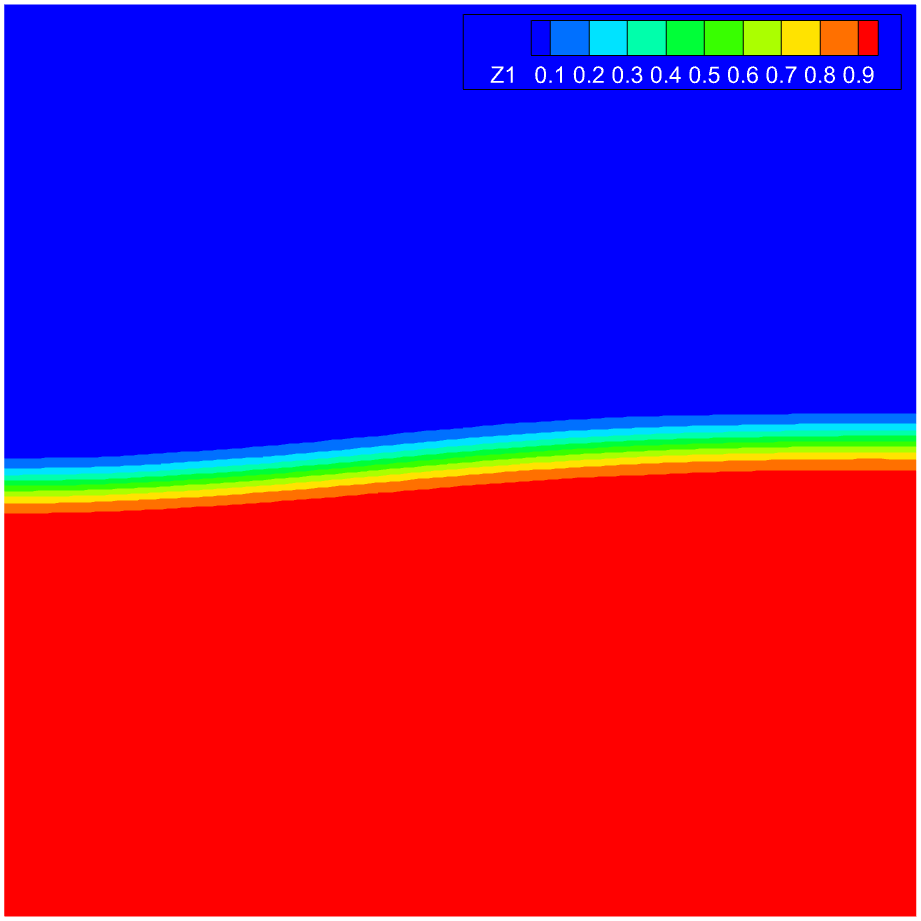
\includegraphics[width=\linewidth]{figure/problem-low-amplitude-standing-wave/z1/wenojs-7.png}
% %     \end{subfigure}
% %     \begin{subfigure}[t]{0.18\linewidth}
% %         \centering
% %         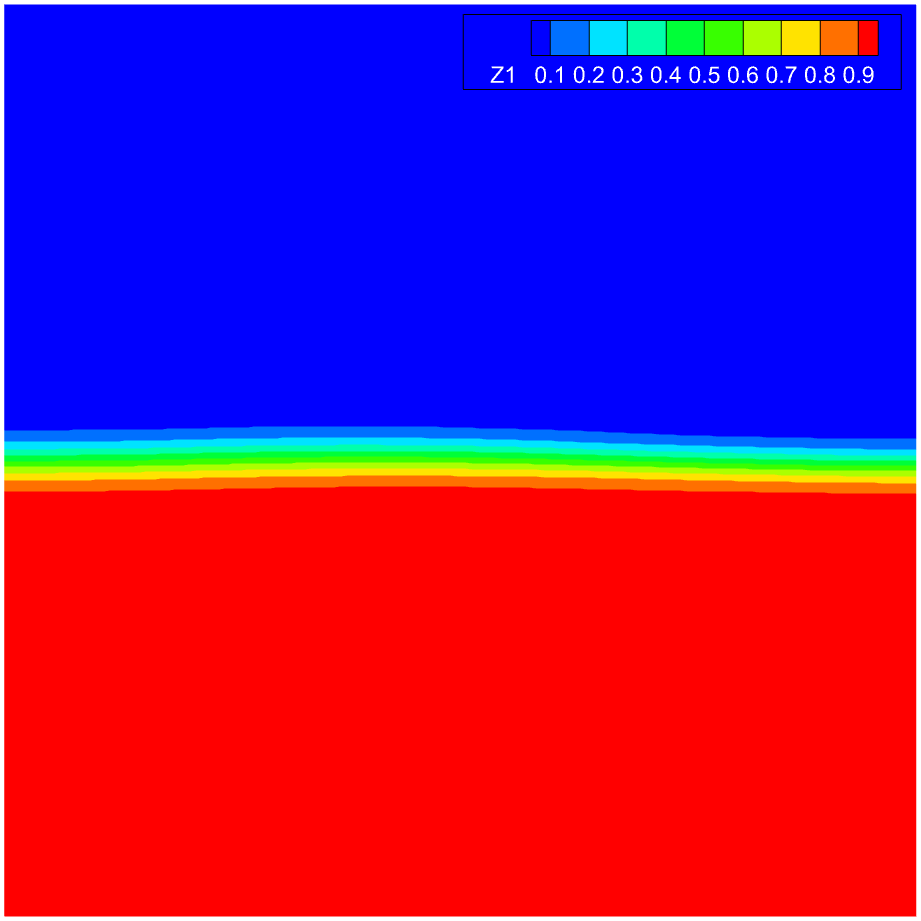
\includegraphics[width=\linewidth]{figure/problem-low-amplitude-standing-wave/z1/wenojs-8.png}
% %     \end{subfigure}
% %     \begin{subfigure}[t]{0.18\linewidth}
% %         \centering
% %         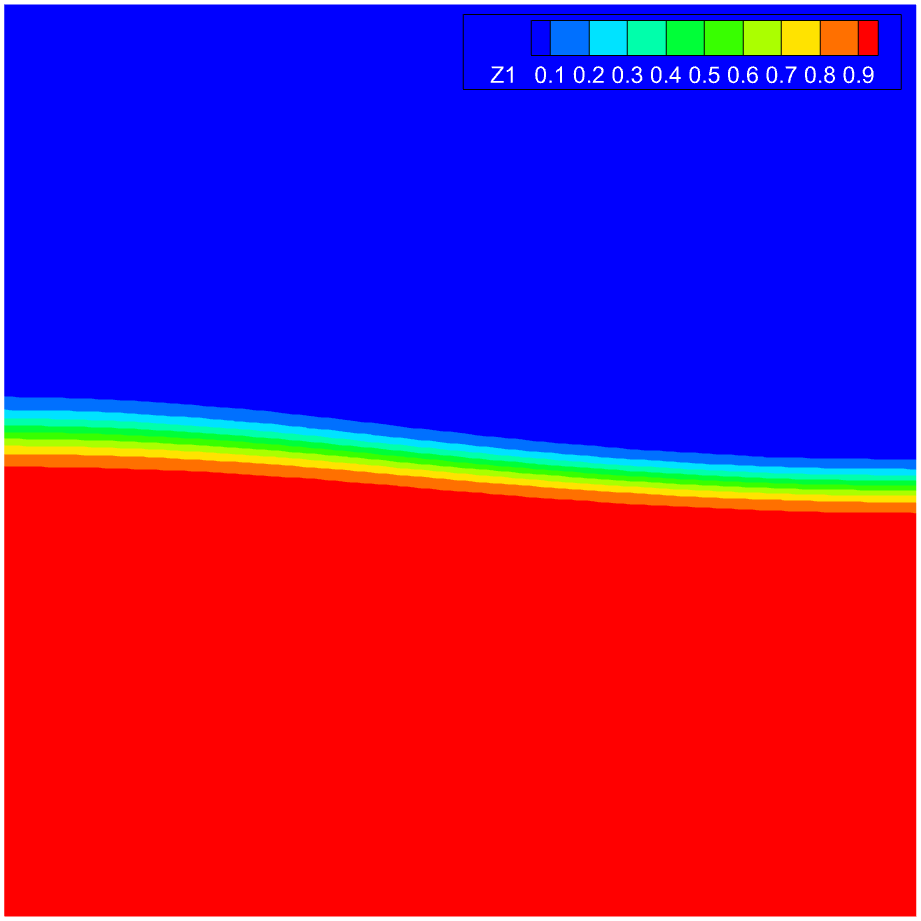
\includegraphics[width=\linewidth]{figure/problem-low-amplitude-standing-wave/z1/wenojs-9.png}
% %     \end{subfigure}
% %     \begin{subfigure}[t]{0.18\linewidth}
% %         \centering
% %         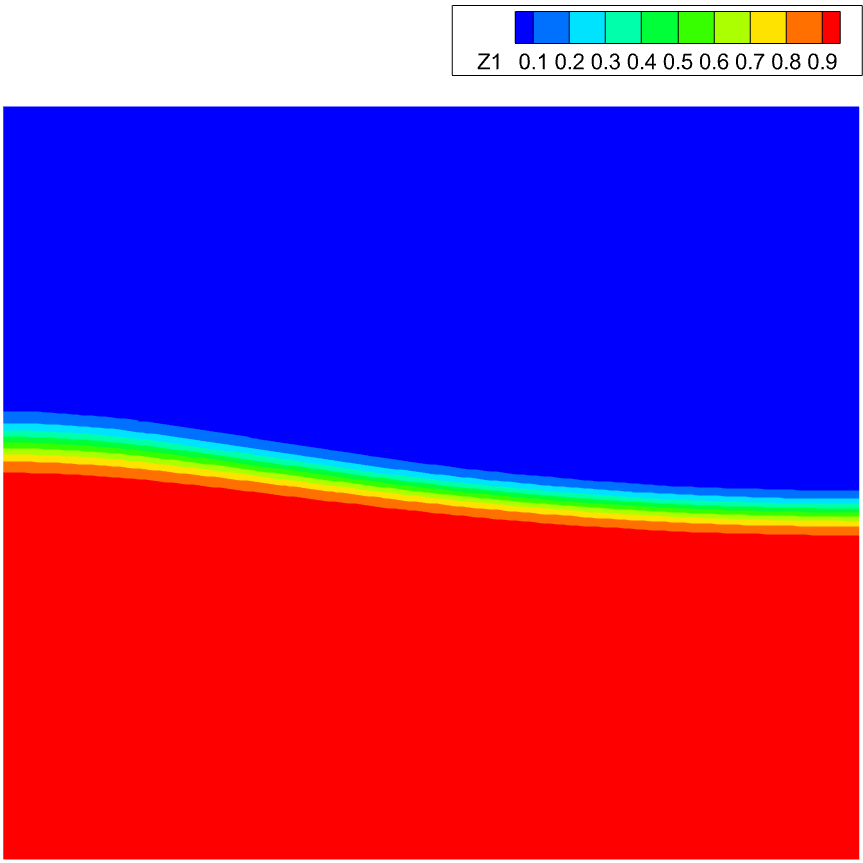
\includegraphics[width=\linewidth]{figure/problem-low-amplitude-standing-wave/z1/wenojs-10.png}
% %     \end{subfigure}\\ 
% %     \caption{$z_1$ 随时间变化，使用WENOEXP方法计算，$128\times 128$}
% %     \label{fig:low-amplitude-standing-wave-exp}
% % \end{figure}


% % 基于二阶小扰动理论~\cite{Frandsen2003}，低幅值自由液面运动的理论振荡周期为$T \approx 1.04~\mathrm{s}$。\autoref{tab:low-amplitude-standing-wave-period} 列出了各网格分辨率下数值计算所得的振荡周期，与参考值同样吻合良好。

% % \begin{table}[!htbp]
% %     \centering
% %     \caption{低幅值驻波问题振荡周期（单位：s）。}
% %     \label{tab:low-amplitude-standing-wave-period}
% %     \begin{tabular}{lccc}
% %         \toprule
% %         网格 & $32 \times 32$ & $64 \times 64$ & $128 \times 128$ \\
% %         \midrule
% %         WENOJS & 1.00 & 1.03 & 1.05 \\
% %         WENOEXP & 1.07 & 1.06 & 1.05 \\
% %         \bottomrule
% %     \end{tabular}
% % \end{table}

% % 图~X 给出了 WENO-JS 与 WENO-EXP 两种格式所得到的体积分数分布。结果表明，由于数值耗散较大，WENO-JS 格式计算所得界面厚度随时间逐渐增加；相比之下，WENO-EXP 格式在相同网格分辨率下，界面厚度在整个模拟过程中基本保持均匀，能够分辨出明显更为锐利的气-水界面，体现了低耗散格式在自由液面流动长时间模拟中的优势。


% % 图~\autoref{fig:standing-wave-interface} 对比了该算例的理论预测界面演化与数值计算结果，其中计算采用 DG-WENO-PP 方法，网格分辨率分别取 $N = 32^2$、$64^2$ 与 $128^2$。结果表明，随着网格单元数的增加，数值结果与理论预测解吻合程度逐渐提高。

% \subsection{线性晃荡问题}
% \begin{figure}[!htbp]
%     \centering
%     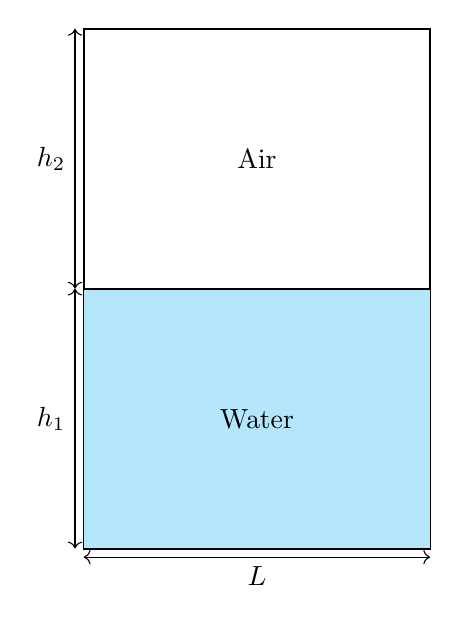
\begin{tikzpicture}[scale=1.1]

% Geometry parameters
\def\L{4}      % width
\def\Hone{3}   % water height h1
\def\Htwo{3}   % air height h2

% Outer boundary
\draw[thick] (0,0) rectangle (\L,\Hone+\Htwo);

% Water region (blue fill)
\fill[cyan!30] (0,0) rectangle (\L,\Hone);

% Interface
\draw[thick] (0,\Hone) -- (\L,\Hone);

% Phase labels
\node at (\L/2,\Hone+\Htwo/2) {Air};
\node at (\L/2,\Hone/2) {Water};


% Height h2
\draw[<->] (-0.1,\Hone) -- (-0.1,\Hone+\Htwo)
node[midway, left] {$h_2$};

% Height h1
\draw[<->] (-0.1,0) -- (-0.1,\Hone)
node[midway, left] {$h_1$};

% Width L
\draw[<->] (0,-0.1) -- (\L,-0.1)
node[midway, below] {$L$};

% % Acceleration a (horizontal)
% \draw[->] (\L+0.6,\Hone+1.2) -- (\L+1.6,\Hone+1.2)
% node[right] {$a$};

% % Gravity g (downward)
% \draw[->] (\L+1.1,\Hone+0.6) -- (\L+1.1,\Hone-0.6)
% node[midway, right] {$g$};

\end{tikzpicture}

%     \caption{}
%     \label{fig:linear-sloshing}
% \end{figure}

% 本算例考虑二维线性晃荡问题~\cite{Chanteperdrix2004,grenier2013accurate}，如~\autoref{fig:linear-sloshing}所示。初始时刻，空气与水在重力作用下于封闭水箱中保持静止，水箱由四个自由滑移固壁组成。当 $t > 0$ 时，在整个流体域内沿 $x$ 轴正方向施加恒定水平加速度 $a$，这等价于水箱以加速度 $-a\bm{e}_x$ 突然沿 $x$ 轴负方向运动的情形。计算域为 $[0, 1~\mathrm{m}] \times [0, 2.25~\mathrm{m}]$，初始水面高度 $h_1 = 1~\mathrm{m}$，初始气层高度 $h_2 = 1.25~\mathrm{m}$，重力加速度 $g = 9.81~\mathrm{m/s^2}$，水平激励加速度 $a = 0.01g$，两相声速均取 $c_1 = c_2 = 100~\mathrm{m/s}$。

% 基于线性化势流理论，界面高度 $\eta(x, t)$ 的解析解为~\cite{Chanteperdrix2004,grenier2013accurate}
% \begin{equation}
%     \eta(x, t) = \frac{a}{g}\left(x - \frac{L}{2} + \sum_{n=0}^{+\infty} \frac{4}{L\kappa_{2n+1}^2}\cos(\omega_{2n+1}t)\cos(\kappa_{2n+1}x)\right),
% \end{equation}
% 其中
% \begin{equation}
%     \kappa_n = \frac{n\pi}{L}, \qquad \omega_n = \sqrt{\frac{g\kappa_n(\rho_{1,0} - \rho_{2,0})}{\rho_{1,0}\coth(\kappa_n h_1) + \rho_{2,0}\coth(\kappa_n h_2)}}.
% \end{equation}

% 图~X 给出了水箱左、右壁处气-水界面高度随时间变化的历程，
% 分别基于三种均匀网格（$64\Delta x \times 144\Delta y$、
% $128\Delta x \times 288\Delta y$ 及 $256\Delta x \times 576\Delta y$）计算得到。
% 图~X 还给出了 $t = 1, 2, 3, 4~\mathrm{s}$ 四个时刻通过
% $z_1 = 0.5$ 等值线绘制的气-水界面形状。
% 数值结果与解析解之间的良好一致性表明，
% 所提出的有限体积 WENO 格式能够准确模拟高密度比条件下
% 含自由液面的线性晃荡流动。


% \subsection{Rayleigh--Taylor 不稳定性问题}
% % \begin{figure}[!htbp]
% %     \centering
% %     \label{fig:}
% %     \input{tikz/}
% %     \caption{}
% % \end{figure}

% \begin{figure}[!htbp]
%     \centering
%      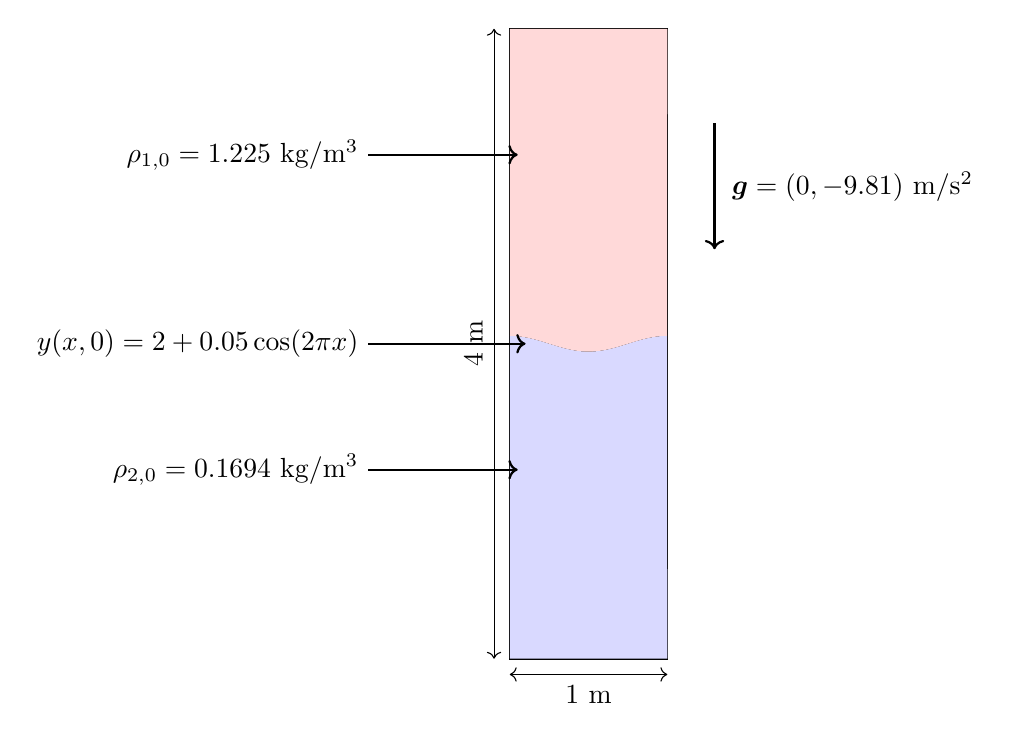
\begin{tikzpicture}[scale=2]

        %=====================
        % Domain
        %=====================
        \draw[thick] (0,0) rectangle (1,4);

        %=====================
        % Interface
        %=====================
        \draw[thick,domain=0:1,samples=200]
        plot (\x,{2 + 0.05*cos(2*pi*\x r)});

        %=====================
        % Fill regions
        %=====================
        \fill[blue!15,domain=0:1,samples=200]
        (0,0)
        -- plot (\x,{2 + 0.05*cos(2*pi*\x r)})
        -- (1,0) -- cycle;

        \fill[red!15,domain=0:1,samples=200]
        (0,4)
        -- plot (\x,{2 + 0.05*cos(2*pi*\x r)})
        -- (1,4) -- cycle;

        %=====================
        % Left-side annotations (densities & interface)
        %=====================

        % Upper fluid density
        \draw[->,thick] (-0.9,3.2) -- (0.05,3.2);
        \node[left,align=right] at (-0.9,3.2)
        {$\rho_{1,0}=1.225~\mathrm{kg/m^3}$};

        % Lower fluid density
        \draw[->,thick] (-0.9,1.2) -- (0.05,1.2);
        \node[left,align=right] at (-0.9,1.2)
        {$\rho_{2,0}=0.1694~\mathrm{kg/m^3}$};

        % Interface function
        \draw[->,thick] (-0.9,2.0) -- (0.1,2.0);
        \node[left,align=right] at (-0.9,2.0)
        {$y(x,0)=2+0.05\cos(2\pi x)$};

        %=====================
        % Gravity annotation (right side)
        %=====================
        \draw[->,thick] (1.3,3.4) -- (1.3,2.6);
        \node[right,align=left] at (1.35,3.0)
        {$\bm g=(0,-9.81)\ \mathrm{m/s^2}$};

        %=====================
        % Dimensions
        %=====================
        \draw[<->] (0,-0.1) -- (1,-0.1);
        \node at (0.5,-0.23) {$1~\mathrm{m}$};

        \draw[<->] (-0.1,0) -- (-0.1,4);
        \node[rotate=90] at (-0.23,2) {$4~\mathrm{m}$};

        %=====================
        % Boundary condition note
        %=====================
        % \node at (0.5,4.25) {Free-slip boundaries};

    \end{tikzpicture}
%     \caption{Schematic of the Rayleigh--Taylor instability test case.}
%     \label{fig:RT_setup}
% \end{figure}

% 本算例通过 Rayleigh--Taylor（RT）不稳定性问题~\cite{1997JCoPh.130..269P}
% 验证所提格式处理复杂界面流动的能力。
% 计算域为 $\Omega = [0, 1~\mathrm{m}] \times [0, 4~\mathrm{m}]$，
% 上层流体密度 $\rho_{1,0} = 1.225~\mathrm{kg/m^3}$（重流体），
% 下层流体密度 $\rho_{2,0} = 0.1694~\mathrm{kg/m^3}$（轻流体），
% 对应 Atwood 数 $\mathrm{At} = (\rho_{1,0} - \rho_{2,0})/(\rho_{1,0} + \rho_{2,0}) \approx 0.76$。
% 初始时刻流体静止，两相界面施加余弦扰动：
% \begin{equation}
%     y(x, 0) = 2 + 0.05\cos(2\pi x).
% \end{equation}
% 重力加速度取 $\bm{g} = (0, -9.81~\mathrm{m/s^2})^\top$，两相声速均设为 $c_1 = c_2 = 100~\mathrm{m/s}$，背景压力 $p_0 = 10{,}000~\mathrm{Pa}$，四周施加自由滑移边界条件，计算网格为 $64 \times 256$。问题构型如~\autoref{fig:RT_setup}所示。

% \autoref{fig:RTI-z1} 给出了采用本文方法在不同时刻的相界面演化云图。结果表明，本文方法能够有效模拟界面扰动的复杂演化过程，并能清晰捕获蘑菇状卷起结构及 Kelvin--Helmholtz 二次不稳定导致的精细涡旋结构。

% % \begin{figure}[htbp]
% %     \centering
% %     \subfloat{
% %         \includegraphics[width=0.14\textwidth]{figure/2D-RTI/z1legend.pdf}
% %     } \hspace{0.5em}
% %     \subfloat{
% %         \includegraphics[width=0.14\textwidth]{figure/2D-RTI/z1legend.pdf}
% %     } \hspace{0.5em}
% %     \subfloat{
% %         \includegraphics[width=0.14\textwidth]{figure/2D-RTI/z1legend.pdf}
% %     } \hspace{0.5em}
% %     \subfloat{
% %         \includegraphics[width=0.14\textwidth]{figure/2D-RTI/z1legend.pdf}
% %     } \hspace{0.5em}
% %     \subfloat{
% %         \includegraphics[width=0.14\textwidth]{figure/2D-RTI/z1legend.pdf}
% %     }\\
% %     \subfloat{
% %         \includegraphics[height = 6cm, width=0.14\textwidth]{figure/2D-RTI/z1-1-2.eps}
% %     } \hspace{0.5em}
% %     \subfloat{
% %         \includegraphics[height = 6cm, width=0.14\textwidth]{figure/2D-RTI/z1-1-4.eps}
% %     } \hspace{0.5em}
% %     \subfloat{
% %         \includegraphics[height = 6cm, width=0.14\textwidth]{figure/2D-RTI/z1-1-6.eps}
% %     } \hspace{0.5em}
% %     \subfloat{
% %         \includegraphics[height = 6cm, width=0.14\textwidth]{figure/2D-RTI/z1-1-8.eps}
% %     } \hspace{0.5em}
% %     \subfloat{
% %         \includegraphics[height = 6cm, width=0.14\textwidth]{figure/2D-RTI/z1-1-10.eps}
% %     }\\
% %     \subfloat{
% %         \includegraphics[height = 6cm, width=0.14\textwidth]{figure/2D-RTI/z1-2-2.eps}
% %     }
% %     \hspace{0.5em}
% %     \subfloat{
% %         \includegraphics[height = 6cm, width=0.14\textwidth]{figure/2D-RTI/z1-2-4.eps}
% %     }
% %     \hspace{0.5em}
% %     \subfloat{
% %         \includegraphics[height = 6cm, width=0.14\textwidth]{figure/2D-RTI/z1-2-6.eps}
% %     }
% %     \hspace{0.5em}
% %     \subfloat{
% %         \includegraphics[height = 6cm, width=0.14\textwidth]{figure/2D-RTI/z1-2-8.eps}
% %     } \hspace{0.5em}
% %     \subfloat{
% %         \includegraphics[height = 6cm, width=0.14\textwidth]{figure/2D-RTI/z1-2-10.eps}
% %     }\\
% %     \subfloat{
% %         \includegraphics[height = 6cm, width=0.14\textwidth]{figure/2D-RTI/z1-3-2.eps}
% %     }
% %     \hspace{0.5em}
% %     \subfloat{
% %         \includegraphics[height = 6cm, width=0.14\textwidth]{figure/2D-RTI/z1-3-4.eps}
% %     } \hspace{0.5em}
% %     \subfloat{
% %         \includegraphics[height = 6cm, width=0.14\textwidth]{figure/2D-RTI/z1-3-6.eps}
% %     } \hspace{0.5em}
% %     \subfloat{
% %         \includegraphics[height = 6cm, width=0.14\textwidth]{figure/2D-RTI/z1-3-8.eps}
% %     }
% %     \hspace{0.5em}
% %     \subfloat{
% %         \includegraphics[height = 6cm, width=0.14\textwidth]{figure/2D-RTI/z1-3-10.eps}
% %     }
% %     \caption{Numerical results for the Rayleigh-Taylor instability problem at $t=0.2, 0.4, 0.6, 0.8, 1.0$ using $N=50\times200$, $100\times400$ and $150\times600$ grids (top to bottom).}
% %     \label{fig:RTI-z1}
% %  \end{figure}

% 图~X 进一步给出了相界面最高位置随时间的演化曲线，
% 并与文献~\cite{1997JCoPh.130..269P}中的参考结果进行对比，
% 两者吻合良好，验证了本文方法的准确性。
% 在无保正限制器的情况下，计算在相界面大变形阶段会因分相密度出现负值而中断，
% 这直接说明了保正算法在高密度比复杂界面流动模拟中的必要性。


% \subsection{溃坝流问题}

% 本算例考虑溃坝流问题，该问题已通过实验~\cite{LOBOVSKY2014407,Martin1952PartIA}和数值方法~\cite{PARAMESWARAN2019405,Yang2020AHF}得到广泛研究，用于评估所提格式在模拟含剧烈相界面变形的弱可压缩两相流中的鲁棒性与精度。
% \begin{figure}[!htbp]
%     \centering
%     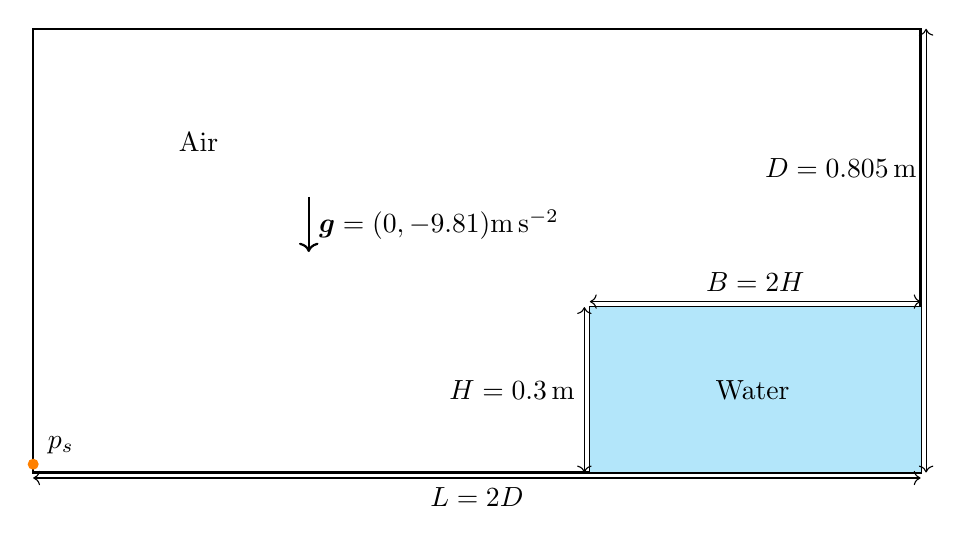
\begin{tikzpicture}[scale=0.7]
    % Draw the container
    \draw[thick] (0, 0) rectangle (16.1, 8.05);
    \draw[thick] (10.1, 0) rectangle (16.1, 3);

    % Fill the water with blue color
    \fill[cyan!30] (10.1, 0) rectangle (16.1, 3);


    % Add labels
    % \node[align=center] at (3, 6) {Air \\ $\rho_{2,0}=\SI{1.0}{\kilogram\per\cubic\meter}$};
    % \node[align=center] at (13.05, 1.5) {Water \\ $\rho_{1,0}=\SI{1000.0}{\kilogram\per\cubic\meter}$};

    % Add labels
    \node[align=center] at (3, 6) {Air};
    \node[align=center] at (13.05, 1.5) {Water};


    \node at (0.5, 0.5) {$p_s$};

    % gravity
    \draw[->, thick] (5,5) -- (5,4)
        node[midway, right] {$\bm{g} = (0, -9.81)\SI{}{\meter\per\second\squared}$};

    % Dimensions and arrows
    \draw[<->] (10.1, 3.1) -- (16.1, 3.1) node[midway, above] {$B = 2H$};
    \draw[<->] (16.2, 0) -- (16.2, 8.05) node[midway, left, yshift=30pt] {$D = \SI{0.805}{\meter}$};
    \draw[<->] (0, -0.1) -- (16.1, -0.1) node[midway, below] {$L = 2D$};
    \draw[<->] (10, 0) -- (10, 3) node[midway, left] {$H = \SI{0.3}{\meter}$};

    % Draw the point p_s
    \fill[orange] (0, 0.15) circle (0.1);

\end{tikzpicture}
%     \caption{溃坝流问题的几何示意图。}
%     \label{fig:dam-break}
% \end{figure}

% 如~\autoref{fig:dam-break}所示，初始时刻一个尺寸为长 $B = 0.6~\mathrm{m}$、高 $H = 0.3~\mathrm{m}$ 的矩形水柱在重力作用下静止，重力加速度为 $\bm{g} = (0, -9.81~\mathrm{m/s^2})^\top$。水柱位于充满空气的矩形容器 $\Omega = [0, 1.61~\mathrm{m}] \times [0, 0.805~\mathrm{m}]$ 中，容器边界施加自由滑移边界条件。压力传感器 $P_s$ 位于容器左壁，其中心距容器底部 $0.015~\mathrm{m}$。计算网格取 $200 \times 400$。

% \autoref{fig:dambreak_interface} 给出了采用 WENO-JS、WENO-EXP 格式在不同时刻的体积分数分布云图，展示了水柱坍塌、水舌向前推进及与右壁碰撞后回溯的完整动态过程。三种格式均成功完成了模拟，均能捕捉到相界面的大变形特征。其中，WENO-EXP 格式在相界面附近引入的数值耗散最小，界面形态的精细结构保持最为完整。

% \begin{figure}[!htbp]
%     \centering
%     \begin{subfigure}[t]{0.3\linewidth}
%         \centering
%         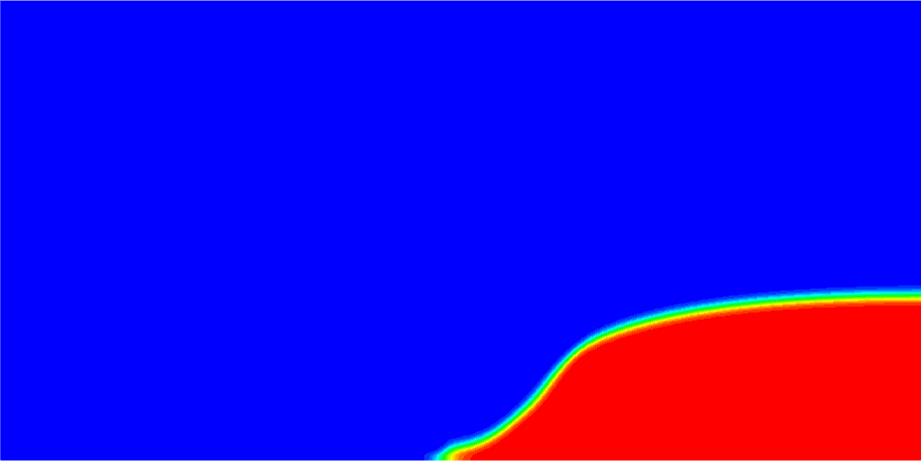
\includegraphics[width=\linewidth]{figure/dambreak/wenojs-1.png}
%         % \label{fig:untitled}
%     \end{subfigure}
%     \begin{subfigure}[t]{0.3\linewidth}
%         \centering
%         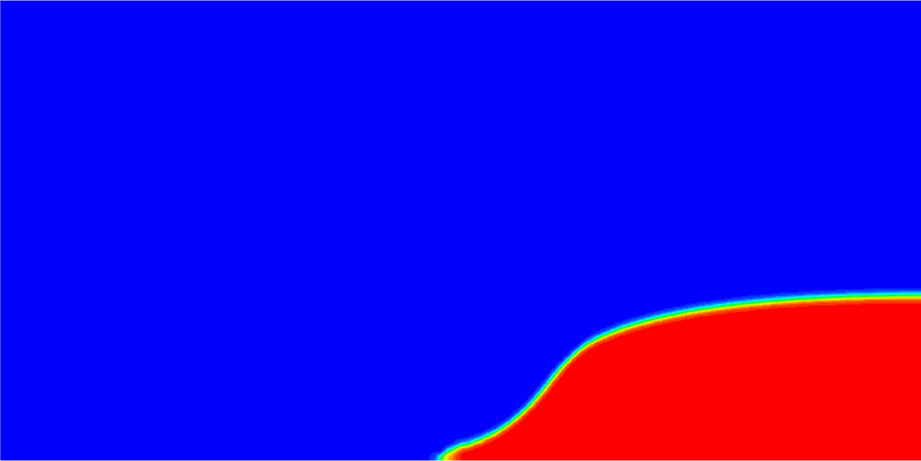
\includegraphics[width=\linewidth]{figure/dambreak/wenoexp1-1.png}
%         % \label{fig:z1}
%     \end{subfigure}
%     \begin{subfigure}[t]{0.3\linewidth}
%         \centering
%         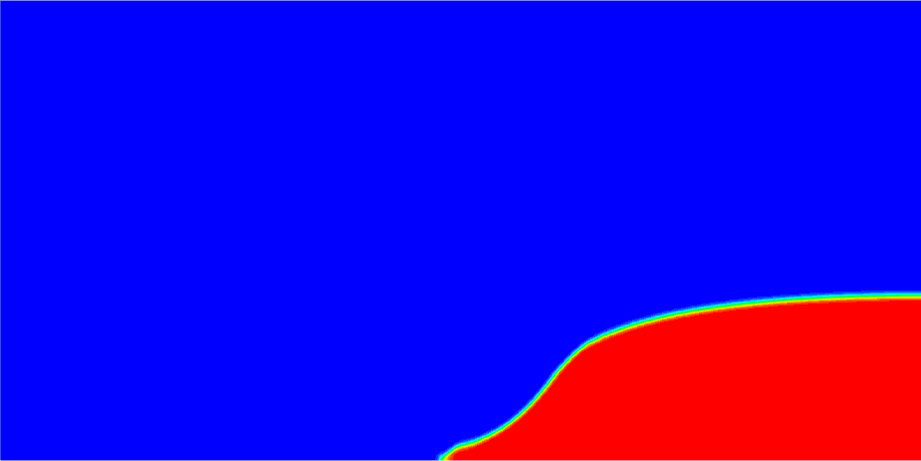
\includegraphics[width=\linewidth]{figure/dambreak/wenoexp2-1.png}
%         % \label{fig:z1}
%     \end{subfigure}\\
%     \begin{subfigure}[t]{0.3\linewidth}
%         \centering
%         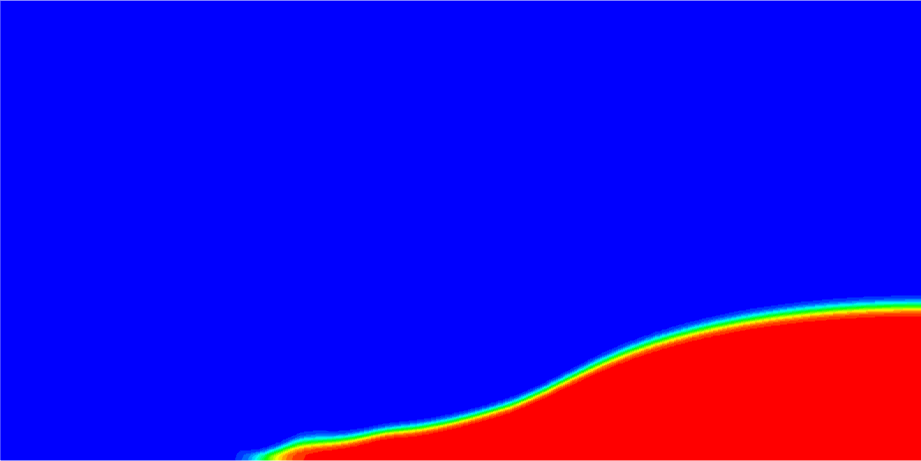
\includegraphics[width=\linewidth]{figure/dambreak/wenojs-2.png}
%         % \label{fig:untitled}
%     \end{subfigure}
%     \begin{subfigure}[t]{0.3\linewidth}
%         \centering
%         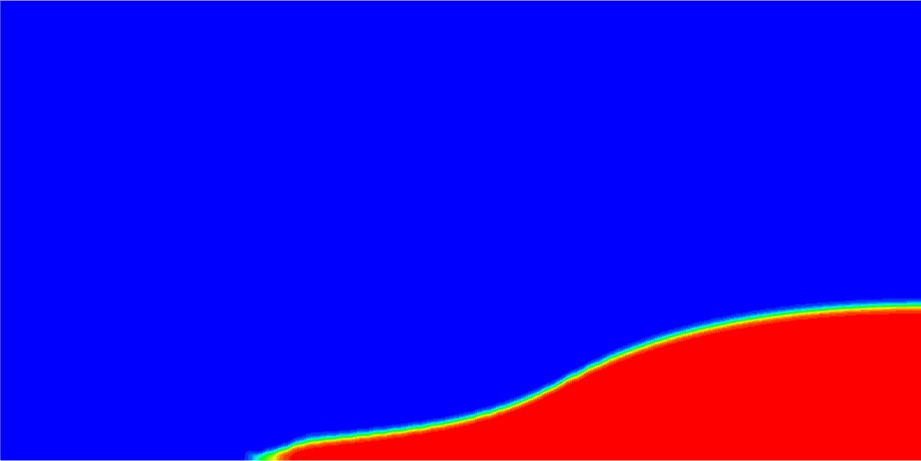
\includegraphics[width=\linewidth]{figure/dambreak/wenoexp1-2.png}
%         % \label{fig:z1}
%     \end{subfigure}
%     \begin{subfigure}[t]{0.3\linewidth}
%         \centering
%         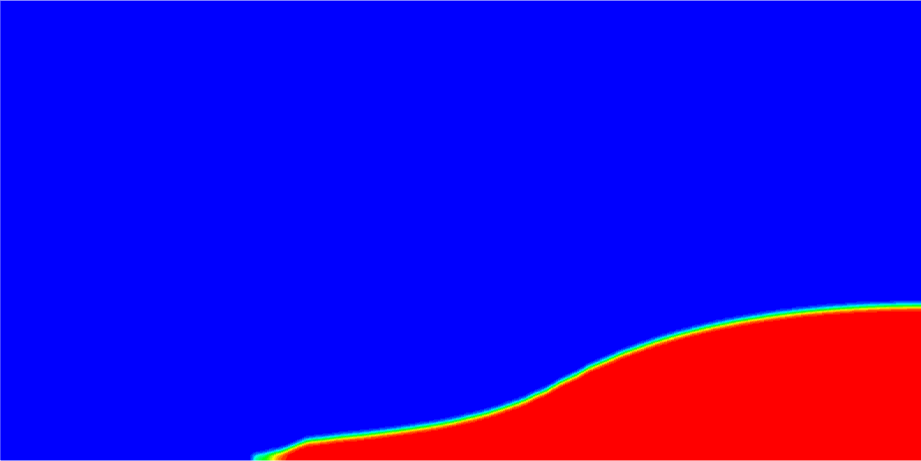
\includegraphics[width=\linewidth]{figure/dambreak/wenoexp2-2.png}
%         % \label{fig:z1}
%     \end{subfigure}\\
%     \begin{subfigure}[t]{0.3\linewidth}
%         \centering
%         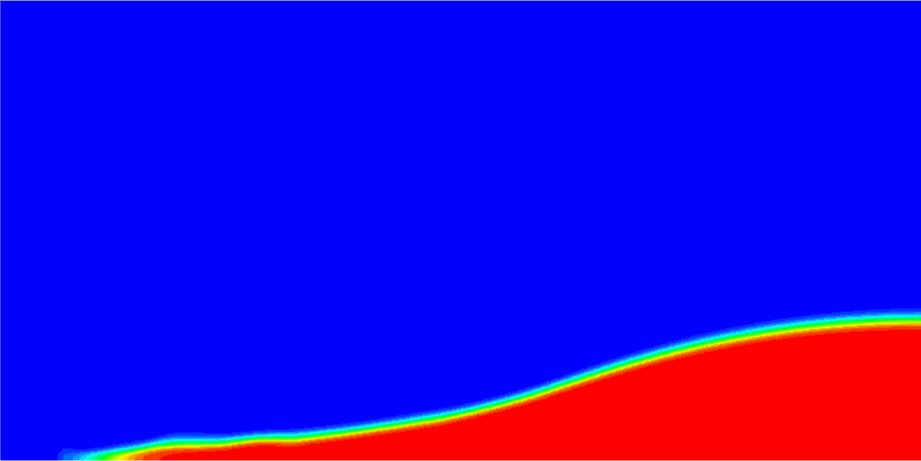
\includegraphics[width=\linewidth]{figure/dambreak/wenojs-3.png}
%         % \label{fig:untitled}
%     \end{subfigure}
%     \begin{subfigure}[t]{0.3\linewidth}
%         \centering
%         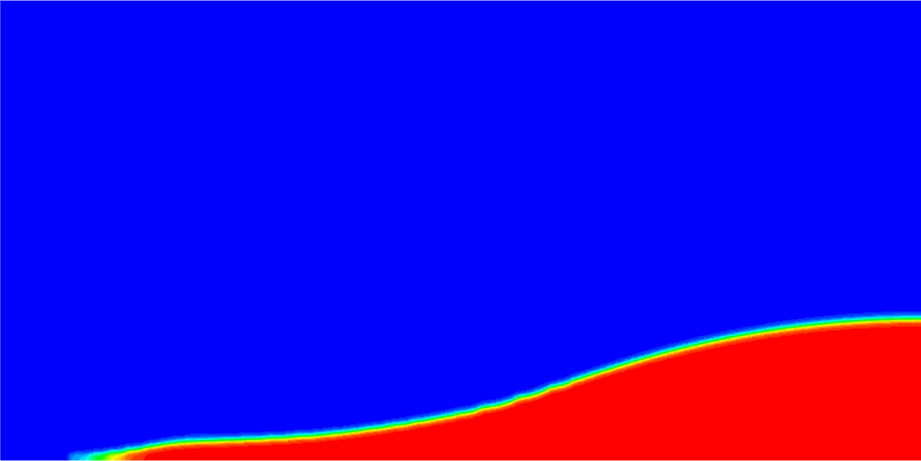
\includegraphics[width=\linewidth]{figure/dambreak/wenoexp1-3.png}
%         % \label{fig:z1}
%     \end{subfigure}
%     \begin{subfigure}[t]{0.3\linewidth}
%         \centering
%         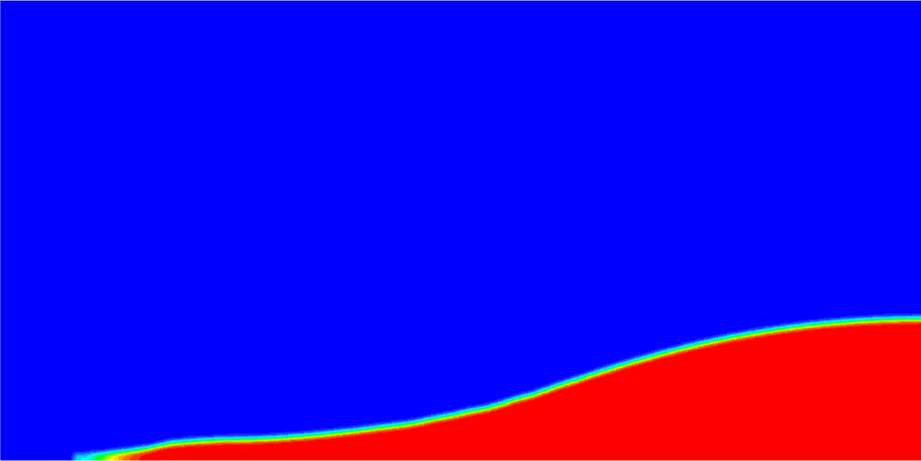
\includegraphics[width=\linewidth]{figure/dambreak/wenoexp2-3.png}
%         % \label{fig:z1}
%     \end{subfigure}\\
%     \begin{subfigure}[t]{0.3\linewidth}
%         \centering
%         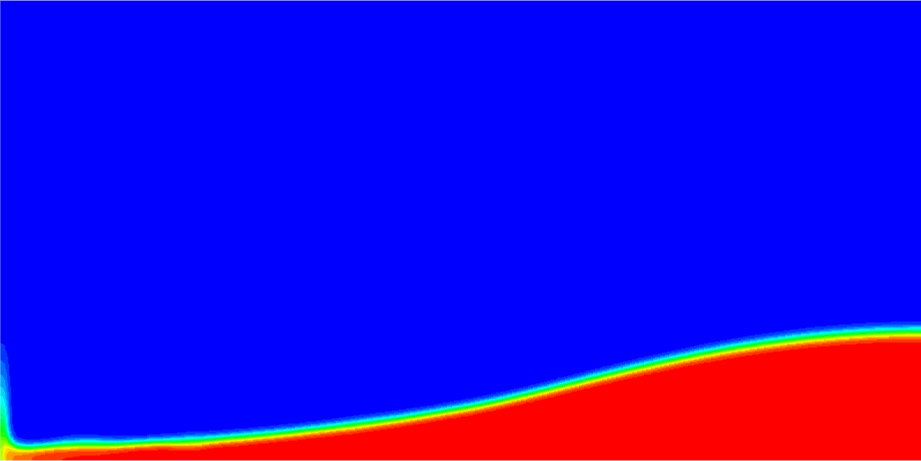
\includegraphics[width=\linewidth]{figure/dambreak/wenojs-4.png}
%         % \label{fig:untitled}
%     \end{subfigure}
%     \begin{subfigure}[t]{0.3\linewidth}
%         \centering
%         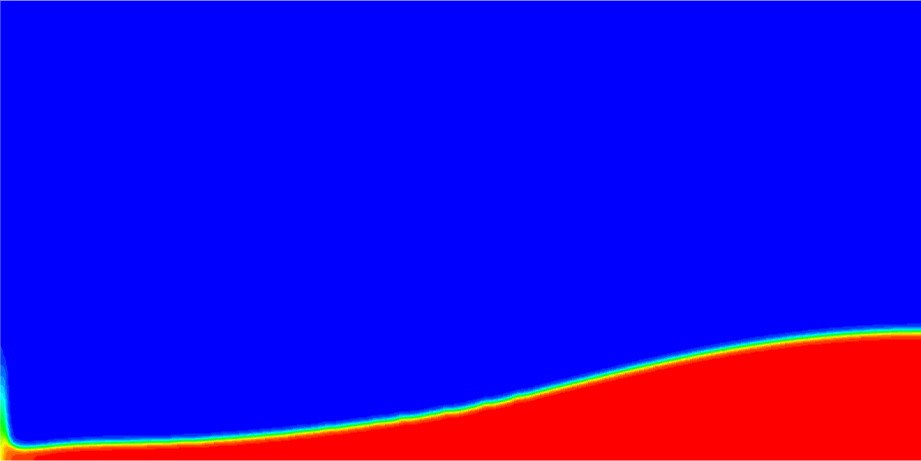
\includegraphics[width=\linewidth]{figure/dambreak/wenoexp1-4.png}
%         % \label{fig:z1}
%     \end{subfigure}
%     \begin{subfigure}[t]{0.3\linewidth}
%         \centering
%         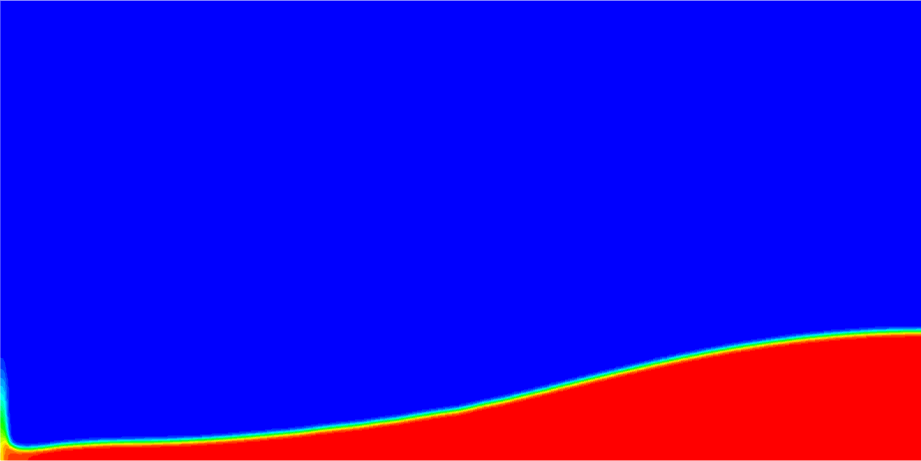
\includegraphics[width=\linewidth]{figure/dambreak/wenoexp2-4.png}
%         % \label{fig:z1}
%     \end{subfigure}\\
%     \begin{subfigure}[t]{0.3\linewidth}
%         \centering
%         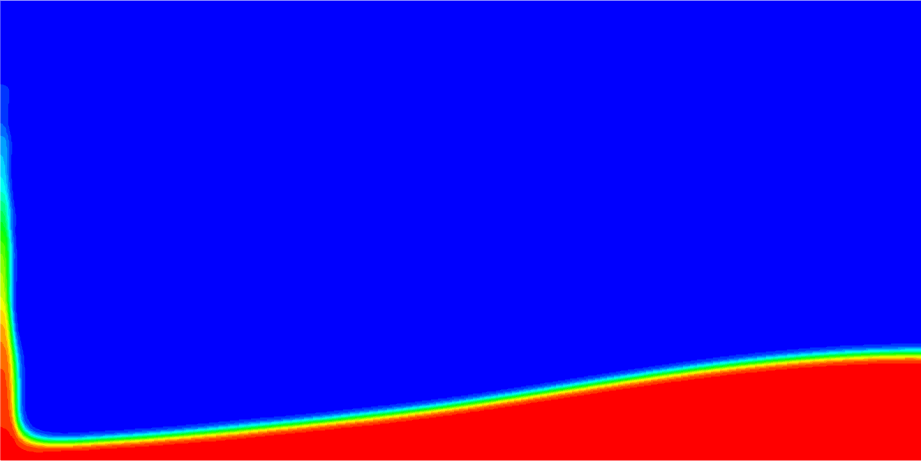
\includegraphics[width=\linewidth]{figure/dambreak/wenojs-5.png}
%         % \label{fig:untitled}
%     \end{subfigure}
%     \begin{subfigure}[t]{0.3\linewidth}
%         \centering
%         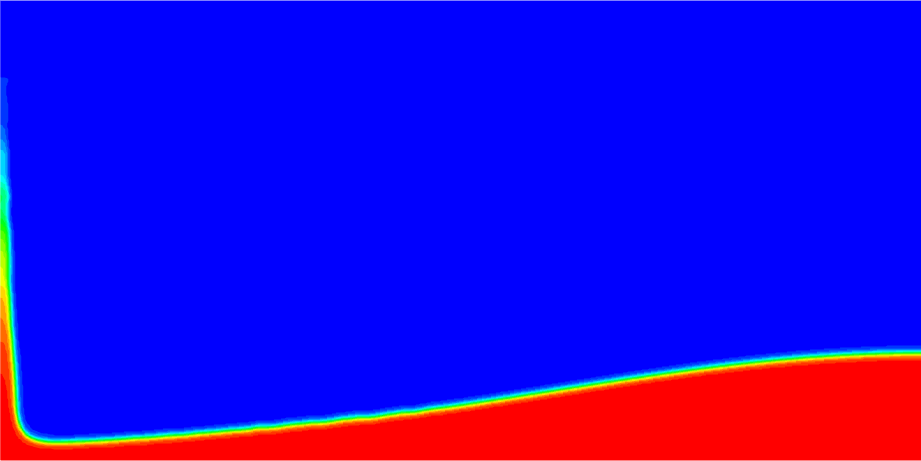
\includegraphics[width=\linewidth]{figure/dambreak/wenoexp1-5.png}
%         % \label{fig:z1}
%     \end{subfigure}
%     \begin{subfigure}[t]{0.3\linewidth}
%         \centering
%         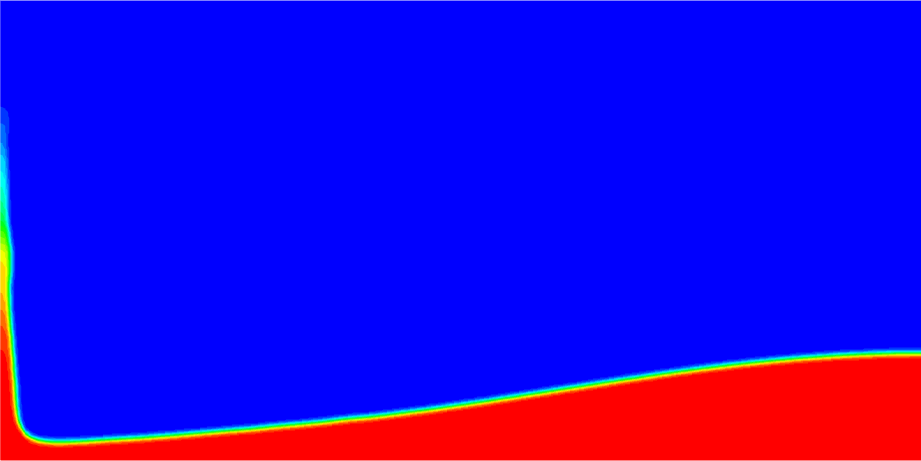
\includegraphics[width=\linewidth]{figure/dambreak/wenoexp2-5.png}
%         % \label{fig:z1}
%     \end{subfigure}\\
%     \begin{subfigure}[t]{0.3\linewidth}
%         \centering
%         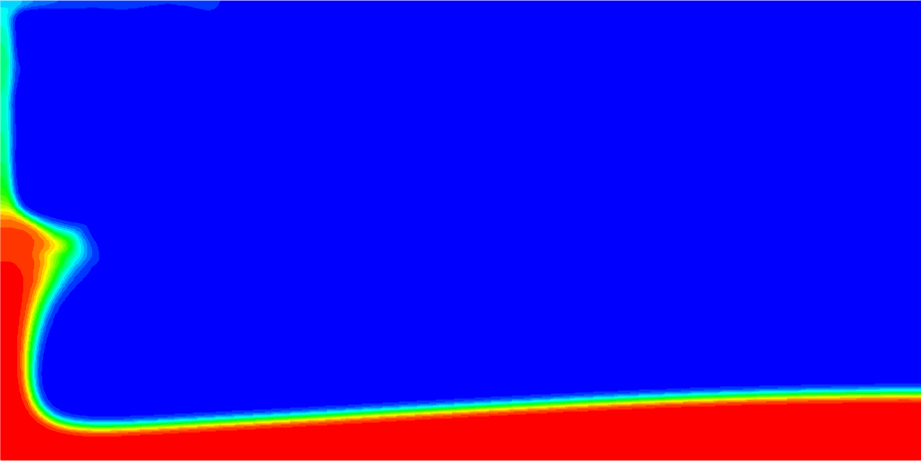
\includegraphics[width=\linewidth]{figure/dambreak/wenojs-6.png}
%         % \label{fig:untitled}
%     \end{subfigure}
%     \begin{subfigure}[t]{0.3\linewidth}
%         \centering
%         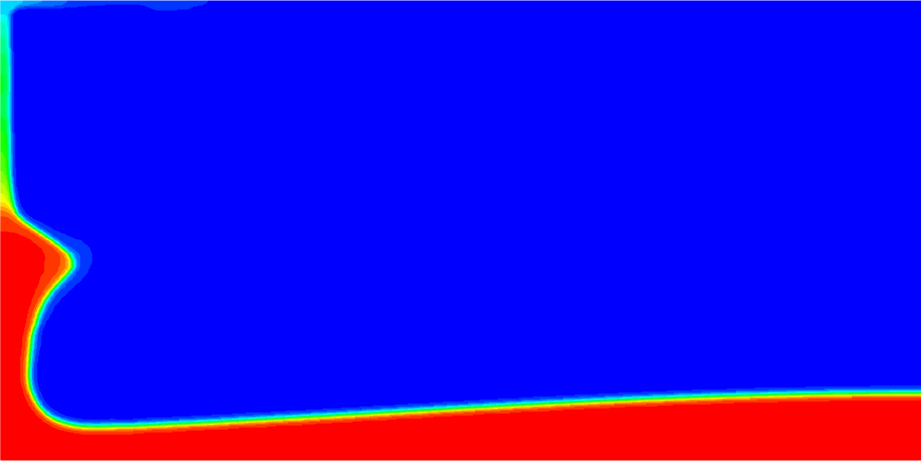
\includegraphics[width=\linewidth]{figure/dambreak/wenoexp1-6.png}
%         % \label{fig:z1}
%     \end{subfigure}
%     \begin{subfigure}[t]{0.3\linewidth}
%         \centering
%         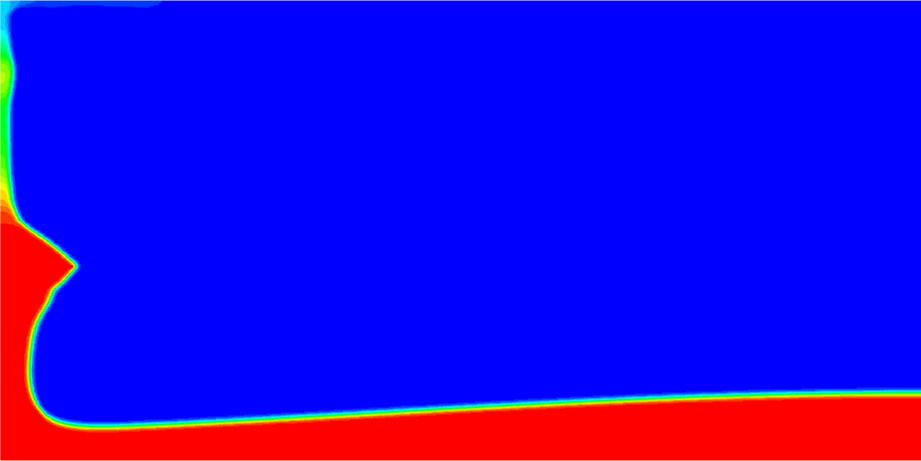
\includegraphics[width=\linewidth]{figure/dambreak/wenoexp2-6.png}
%         % \label{fig:z1}
%     \end{subfigure}\\
%     \begin{subfigure}[t]{0.3\linewidth}
%         \centering
%         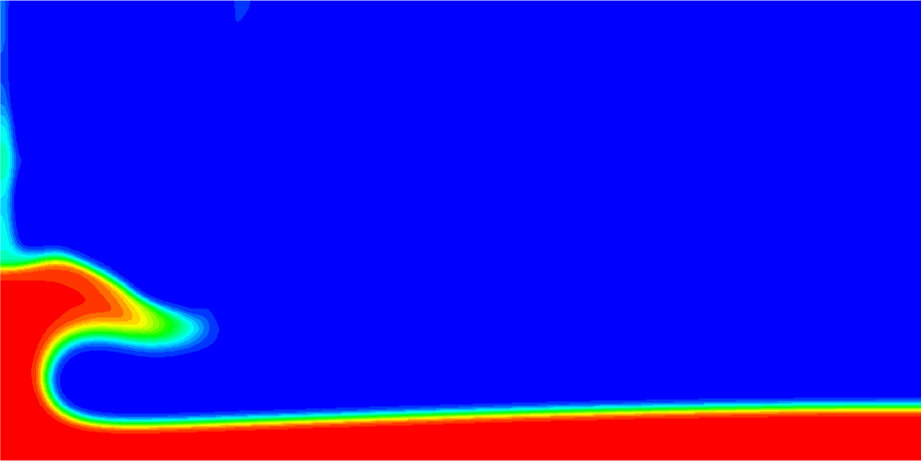
\includegraphics[width=\linewidth]{figure/dambreak/wenojs-7.png}
%         % \label{fig:untitled}
%     \end{subfigure}
%     \begin{subfigure}[t]{0.3\linewidth}
%         \centering
%         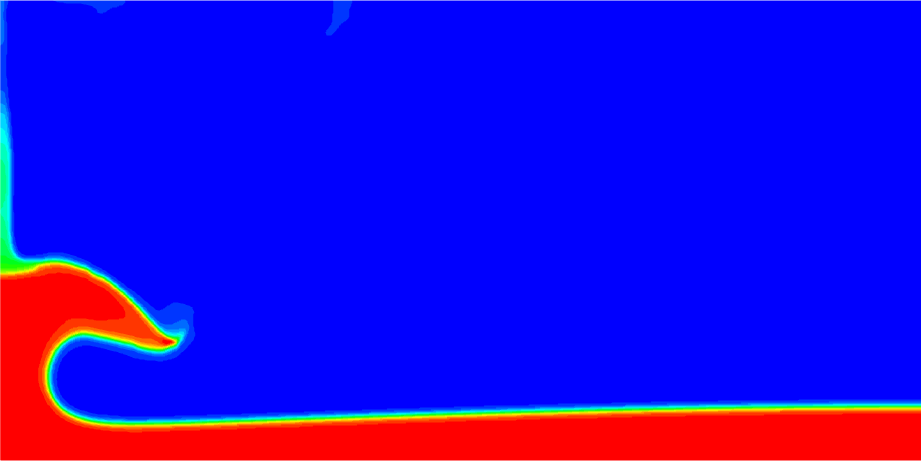
\includegraphics[width=\linewidth]{figure/dambreak/wenoexp1-7.png}
%         % \label{fig:z1}
%     \end{subfigure}
%     \begin{subfigure}[t]{0.3\linewidth}
%         \centering
%         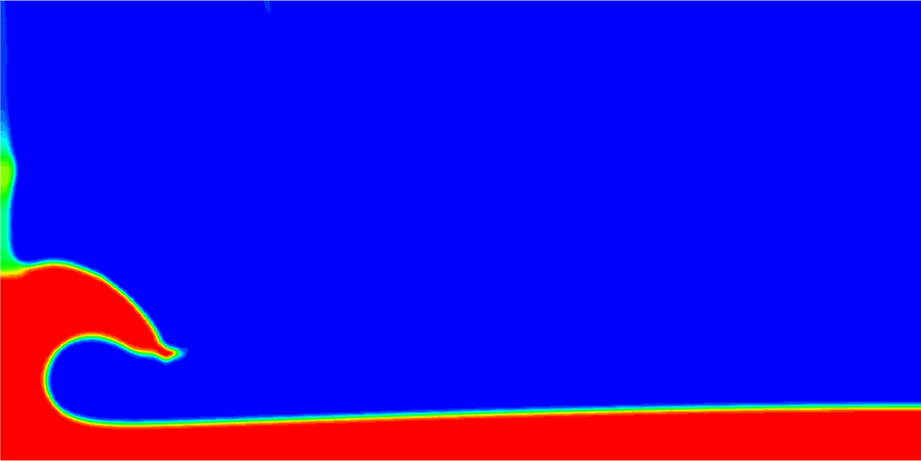
\includegraphics[width=\linewidth]{figure/dambreak/wenoexp2-7.png}
%         % \label{fig:z1}
%     \end{subfigure}\\
%     \begin{subfigure}[t]{0.3\linewidth}
%         \centering
%         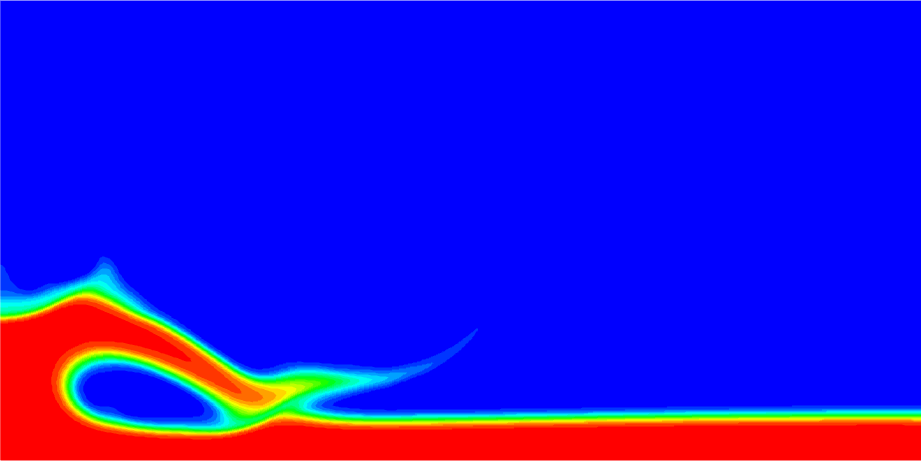
\includegraphics[width=\linewidth]{figure/dambreak/wenojs-8.png}
%         % \label{fig:untitled}
%     \end{subfigure}
%     \begin{subfigure}[t]{0.3\linewidth}
%         \centering
%         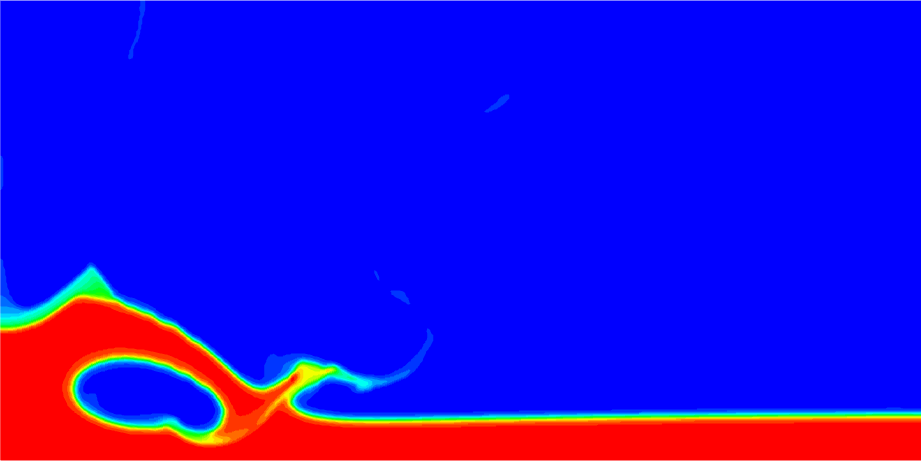
\includegraphics[width=\linewidth]{figure/dambreak/wenoexp1-8.png}
%         % \label{fig:z1}
%     \end{subfigure}
%     \begin{subfigure}[t]{0.3\linewidth}
%         \centering
%         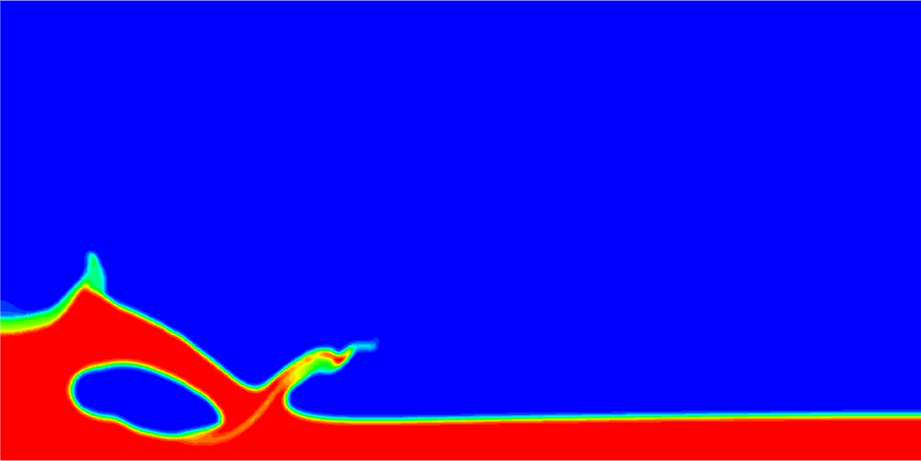
\includegraphics[width=\linewidth]{figure/dambreak/wenoexp2-8.png}
%         % \label{fig:z1}
%     \end{subfigure}\\
%     \caption{从左到右：WENOJS,WENOEXP1, WENOEXP2. 200x400}
%     \label{fig:dambreak_interface}
% \end{figure}


% 图~X 给出了压力传感器处压力随时间的变化曲线，三种格式的数值结果均在合理范围内，与实验数据~\cite{LOBOVSKY2014407}吻合良好，进一步验证了本文格式的准确性与实用性。值得指出的是，在不启用保正限制器的情况下，计算会因界面大变形导致分相密度出现负值而崩溃，再次证明了保正算法在含大密度比剧烈两相流问题中的重要性。

\cleardoublepage
\section{结论与展望}

本文针对弱可压缩不混溶两相流的高精度数值模拟问题，
以三方程模型为控制方程框架，提出了一种基于指数多项式逼近空间的
有限体积 WENO 格式，并配套设计了保正限制算法。主要研究工作与结论如下。

在数学模型方面，本文采用由两相质量守恒方程与混合物动量守恒方程
构成的三方程弱可压缩两相流模型，结合等熵状态方程与瞬时压力平衡假设
对方程组进行封闭。通过特征分析证明，当分相密度严格为正时，
控制方程系统保持双曲性，且混合声速为实数，
由此确立了数值格式保正性设计的物理基础。
平衡体积分数的显式求解公式表明，方程组存在唯一有效的物理可容许解，
为数值实现提供了严格保证。

在数值格式方面，本文提出了基于指数多项式逼近空间的
有限体积 WENO 重构格式（WENO-EXP）。
该格式的核心思想在于通过局部优化指数函数中的形状参数，
在不扩大重构模板的前提下将精度提升一阶：
WENO-EXP-I 格式实现了与传统五阶 WENO 格式相当的精度，
而 WENO-EXP-II 格式进一步实现了六阶收敛精度。
通过分析形状参数与 WENO 线性权重之间的关系，
本文推导了形状参数的上界条件，以确保线性权重的非负性，
从而保证重构格式的数值稳定性。

在速度压力平衡性方面，本文证明了基于 LLF 通量、HLLC 通量的有限体积格式
以及特征变量重构策略均满足 Abgrall 原则，
即在孤立相界面对流过程中能够严格保持均匀压力与速度剖面，
有效避免了由体积分数梯度引起的非物理寄生振荡。

在保正算法方面，本文针对非多项式逼近空间设计了两相分相密度的
保正限制算法。通过将单元平均守恒变量表示为凸分解形式，
并结合适当的 CFL 条件，严格证明了在满足保正条件的前提下，
单元平均值在每个时间步内保持在物理可容许集内。
缩放型保正限制器的设计同时保证了界面处均匀压力与速度分布的保持。

数值算例验证结果表明，所提出的格式在以下几方面表现优异：
在光滑对流问题中，WENO-EXP-II 格式在一维和二维情形下均实现了
预期的六阶收敛精度，优于传统五阶 WENO-JS 格式；
在锐利界面对流、Zalesak 刚性旋转等考验界面捕获精度的算例中，
WENO-EXP 格式在保持无振荡特性的同时，相界面厚度更薄、轮廓更锐利；
在低幅值驻波、线性晃荡等含自由液面的水动力学问题中，
所提格式的数值结果与解析解吻合良好，体现了其在长时间积分中的低耗散特性；
在 Rayleigh--Taylor 不稳定性和溃坝流等含大密度比、
剧烈相界面变形的挑战性问题中，保正算法保障了计算的鲁棒性，
能够清晰捕获复杂涡旋结构与大变形界面形态。

本文工作尚存在以下不足，有待在后续研究中进一步完善：

其一，本文所采用的三方程弱可压缩模型不包含能量方程，
因此不适用于涉及热效应或相变的两相流问题。
将本文格式推广至包含能量方程的可压缩两相流模型（如五方程模型）
是一个自然的研究方向，相关工作已在文献~\cite{Zhang2025exponential}中
针对可压缩情形有所探索，但弱可压缩框架下的推广仍有待开展。

其二，本文仅考虑了无粘流动，实际工程问题中往往需要考虑粘性效应
与表面张力的影响。将本文格式与粘性项离散及表面张力模型相结合，
是提升方法适用范围的重要课题。

其三，本文当前实现基于结构化均匀矩形网格，
将格式推广至非结构网格或自适应网格上，
以处理具有复杂几何边界的实际工程问题，也是值得探索的方向。

其四，本文的时间离散采用显式 SSP-RK 方法，受弱可压缩模型声速较大的限制，时间步长受到严格的 CFL 约束，计算效率有待进一步提升。发展半隐式或隐显（IMEX）时间推进方案以放宽时间步长限制，是提高弱可压缩两相流计算效率的重要途径。

\cleardoublepage
\bibliographystyle{unsrt}
\bibliography{ref}

\cleardoublepage
\section{攻读学位期间学术成果及获奖情况}
\paragraph{学术成果}
\begin{itemize}
  \item \textbf{Z. Yang} and Z Fan* \\ 
  A positivity-preserving HLLC-based discontinuous Galerkin method for weakly compressible two-phase flows \\ 
  \textbf{Journal of Computational and Applied Mathematics}, 462:116467, 2025
  \item Z. Fan*, \textbf{Z. Yang}, C. Jian, L. Tiegang \\
  Exponential approximation space based finite volume WENO scheme for solving the five-equation model of compressible two-medium flows\\ 
  \textbf{Journal of Scientific Computing}, 104:6, 2025 
\end{itemize}
\paragraph{获奖情况}
\begin{itemize}
      \item 2023\kern0pt{}年获北京科技大学学业奖学金
      \item 2024\kern0pt{}年获北京科技大学三好研究生
      \item 2024\kern0pt{}年获北京科技大学二等学业奖学金
      \item 2025\kern0pt{}年获硕士研究生国家奖学金
      \item 2025\kern0pt{}年获北京科技大学优秀三好研究生
      \item 2025\kern0pt{}年获北京科技大学一等学业奖学金
\end{itemize}



\cleardoublepage

\section{致谢}
感谢先行者，是本文所引用的各项研究成果和导师、读研以来的各位老师们、父母家人们共同塑造了这篇文章，也塑造了我。

感谢后来者，你们未来的每一次引用和借鉴都是这项研究的意义得以拓宽和生命得以延续的关键。

感谢同行者，求学以来的各位同窗，一起努力，学习奋斗的经历永怀在心。最后，特别感谢孙阳女士对我读研以来的支持。

\cleardoublepage

% \appendix
% \begin{appendix}


% \section{数值微分}

% 对于均匀网格，设网格间距为 $h$，
% 单元平均值记为 $\overline{u}_j$，
% 则以下六点差分算子给出了半整数点处的五阶导数近似：
% \begin{equation}
%     \mathbb{D}_5
%     = -\overline{u}_{j-2} + 5\overline{u}_{j-1} - 10\overline{u}_j
%     + 10\overline{u}_{j+1} - 5\overline{u}_{j+2} + \overline{u}_{j+3},
% \end{equation}
% 其 Taylor 展开给出
% \begin{equation}
%     \frac{\mathbb{D}_5}{h^5}
%     = u^{(5)}(x_{j+1/2})
%     + \frac{u^{(7)}(x_{j+1/2})}{4}\,h^2 + \mathcal{O}(h^3).
% \end{equation}
% 上述结果可用于局部估计解的五阶导数信息，
% 进而计算 WENO-EXP 格式中的形状参数 $\lambda^2\Delta x^2$。
% 以下给出推导该数值微分公式的 MATLAB 程序。

% \section{数值误差范数}

% 设计算域被划分为 $N$ 个均匀网格单元，
% $u_j^{\text{num}}$ 和 $u_j^{\text{exact}}$ 分别为
% 第 $j$ 个单元中心处的数值解与精确解，
% 则数值误差的各阶范数定义为：
% \begin{equation}
%     \begin{aligned}
%         L^1\text{-误差}   & = \frac{1}{N}\sum_{j=1}^{N}\bigl|u_j^{\text{num}} - u_j^{\text{exact}}\bigr|,                             \\[4pt]
%         L^2\text{-误差}   & = \sqrt{\frac{1}{N}\sum_{j=1}^{N}\bigl(u_j^{\text{num}} - u_j^{\text{exact}}\bigr)^2},                    \\[4pt]
%         L^\infty\text{-误差} & = \max_{1\leqslant j\leqslant N}\bigl|u_j^{\text{num}} - u_j^{\text{exact}}\bigr|.
%     \end{aligned}
% \end{equation}
% 注意，此处各范数均对网格数 $N$ 进行了归一化处理，
% 不可直接使用向量的代数范数（未归一化）代替。

% 相邻两次加密计算之间的收敛阶由下式估计：
% \begin{equation}
%     \text{收敛阶}
%     = -\frac{\ln\!\left(\text{Error}^{(q+1)} / \text{Error}^{(q)}\right)}
%     {\ln\!\left(N^{(q)} / N^{(q+1)}\right)},
% \end{equation}
% 其中上标 $(q)$ 表示第 $q$ 次网格加密计算，
% $N^{(q)}$ 和 $\text{Error}^{(q)}$ 分别为对应的网格数与数值误差。
% 该公式适用于结构化均匀网格。

% \end{appendix}

\section{这里放置一些可能有用可能没用的附录内容}
\subsection{黎曼求解器}
下面证明，采用 LLF 格式的有限体积法满足 Abgrall 原则。

\begin{theorem}[LLF 格式的速度压力平衡性]
    \label{thm:llf}
    在无外力条件下，采用 LLF 数值通量~\eqref{eq:llf}的有限体积格式
    ~\eqref{eq:fv_euler}能够在孤立相界面对流过程中保持均匀压力与速度剖面，即：
    \begin{equation}
        \text{若}\quad p^n \equiv p_0,\quad \bm{u}^n \equiv \bm{u}_0,
        \quad\text{则}\quad
        p^{n+1} \equiv p_0,\quad \bm{u}^{n+1} \equiv \bm{u}_0,
        \quad \forall\, I_{i,j} \in \Omega.
    \end{equation}
\end{theorem}

\begin{proof}
不失一般性，考虑一维情形。设初始压力场与速度场均匀，即
$p(x, t^n) \equiv p_0$，$u(x, t^n) \equiv u_0$，
而体积分数场 $z_1(x, t^n)$ 在空间上可以任意分布。
由等熵状态方程~\eqref{eq:eos_single}及均匀压力条件，可知
各相密度处处等于参考密度，即 $\rho_k \equiv \rho_{k,0}$（$k = 1, 2$），
从而分相密度满足 $\tilde{\rho}_k = z_k \rho_{k,0}$。

\textbf{第一步：验证压力保持性。}

对第 $k$ 个分相密度方程施加前向 Euler 时间离散，得到
\begin{equation}
    \label{eq:rho_update}
    \overline{(\tilde{\rho}_k)}_{i}^{n+1}
    = \overline{(\tilde{\rho}_k)}_{i}^{n}
    - \frac{\Delta t}{\Delta x}
    \left[
        \hat{F}_x\!\left((\tilde{\rho}_k u)_L,\, (\tilde{\rho}_k u)_R\right)\big|_{i+1/2}
        -
        \hat{F}_x\!\left((\tilde{\rho}_k u)_L,\, (\tilde{\rho}_k u)_R\right)\big|_{i-1/2}
    \right].
\end{equation}
在均匀压力与速度条件下，通过 WENO 重构得到
$u_L = u_R = u_0$，$\rho_{k,L} = \rho_{k,R} = \rho_{k,0}$，
而 $z_{k,L}$、$z_{k,R}$ 则分别为 $z_k$ 在界面处的左、右重构值。
LLF 通量~\eqref{eq:llf}中分相密度方程的数值通量化简为
\begin{equation}
    \hat{F}_x\!\left((\tilde{\rho}_k u)_L,\, (\tilde{\rho}_k u)_R\right)
    = \frac{1}{2}\bigl[(z_{k,L} + z_{k,R})\rho_{k,0} u_0\bigr]
    - \frac{S_x}{2}\rho_{k,0}(z_{k,R} - z_{k,L})
    = \rho_{k,0}
    \left[
        u_0 \avg{z_k} - \frac{S_x}{2}\jump{z_k}
    \right],
\end{equation}
其中 $\avg{z_k} = (z_{k,L} + z_{k,R})/2$ 为算术平均，
$\jump{z_k} = z_{k,R} - z_{k,L}$ 为跳量。
将式~\eqref{eq:rho_update}代入，得
\begin{equation}
    \overline{(\tilde{\rho}_k)}_{i}^{n+1}
    = \rho_{k,0}
    \left[
        \overline{z_k}_{i}^{n}
        - \frac{\Delta t}{\Delta x}
        \left(
        u_0 \avg{z_k}\big|_{i+1/2} - \frac{S_x}{2}\jump{z_k}\big|_{i+1/2}
        - u_0 \avg{z_k}\big|_{i-1/2} + \frac{S_x}{2}\jump{z_k}\big|_{i-1/2}
        \right)
    \right]
    \eqqcolon \rho_{k,0}\, \overline{z_k}_{i}^{n+1}.
\end{equation}
因此有 $\tilde{\rho}_k^{n+1} = \rho_{k,0}\, z_k^{n+1}$，即
$\rho_k^{n+1} = \tilde{\rho}_k^{n+1} / z_k^{n+1} = \rho_{k,0}$。
再由等熵状态方程~\eqref{eq:eos_single}，立即得到
$p^{n+1} = p_0 + c_k^2(\rho_k^{n+1} - \rho_{k,0}) \equiv p_0$，
压力保持性得证。

此外，验证 $z_1^{n+1} + z_2^{n+1} = 1$：
\begin{equation}
    z_1^{n+1} + z_2^{n+1}
    = \overline{z_1}_i^n + \overline{z_2}_i^n
    - \frac{\Delta t}{\Delta x}
    \left(
        u_0 \avg{z_1 + z_2}\big|_{i+1/2} - \frac{S_x}{2}\jump{z_1+z_2}\big|_{i+1/2}
        - \cdots
    \right).
\end{equation}
由于 $z_1 + z_2 \equiv 1$，有 $\avg{z_1+z_2} = 1$，
$\jump{z_1+z_2} = 0$，从而
\begin{equation}
    z_1^{n+1} + z_2^{n+1}
    = 1 - \frac{\Delta t}{\Delta x}
    \left(
        u_0 \cdot 1\big|_{i+1/2} - u_0 \cdot 1\big|_{i-1/2}
    \right)
    = 1,
\end{equation}
体积分数约束在离散层面精确保持。

\textbf{第二步：验证速度保持性。}

在均匀压力与速度条件下，混合动量方程的数值通量为
\begin{equation}
    \hat{F}_x(\rho u^2 + p)
    = \frac{1}{2}\bigl[(\rho_L u_0^2 + p_0) + (\rho_R u_0^2 + p_0)\bigr]
    - \frac{S_x}{2}(\rho_R - \rho_L) u_0
    = \avg{\rho} u_0^2 + p_0 - \frac{S_x}{2}\jump{\rho}\, u_0,
\end{equation}
其中 $\avg{\rho} = (z_{1,L}\rho_{1,0} + z_{2,L}\rho_{2,0}
+ z_{1,R}\rho_{1,0} + z_{2,R}\rho_{2,0})/2$，
$\jump{\rho} = \rho_R - \rho_L$。
因此，动量更新为
\begin{equation}
    \overline{(\rho u)}_{i}^{n+1}
    = \overline{(\rho u)}_{i}^{n}
    - \frac{\Delta t}{\Delta x}
    \left[
        \left(\avg{\rho} u_0^2 + p_0 - \frac{S_x}{2}\jump{\rho} u_0\right)\bigg|_{i+1/2}
        - \left(\avg{\rho} u_0^2 + p_0 - \frac{S_x}{2}\jump{\rho} u_0\right)\bigg|_{i-1/2}
    \right].
\end{equation}
注意到压力项 $p_0$ 在左右界面抵消，上式整理为
\begin{equation}
    \overline{(\rho u)}_{i}^{n+1}
    = u_0 \left[
        \overline{\rho}_{i}^{n}
        - \frac{\Delta t}{\Delta x}
        \left(
            \avg{\rho} u_0 - \frac{S_x}{2}\jump{\rho}
        \bigg|_{i+1/2}
            -
            \avg{\rho} u_0 - \frac{S_x}{2}\jump{\rho}
        \bigg|_{i-1/2}
        \right)
    \right]
    = u_0\, \overline{\rho}_{i}^{n+1}.
\end{equation}
最后一个等号利用了密度更新方程（即将两相分相密度方程对 $k=1,2$ 求和）。
从而 $u^{n+1} = \overline{(\rho u)}_i^{n+1} / \overline{\rho}_i^{n+1} = u_0$，
速度保持性得证。
\end{proof}

HLLC 格式同样满足 Abgrall 原则，具体陈述如下。

\begin{theorem}[HLLC 格式的速度压力平衡性~\cite{zhang2025positivity}]
    \label{thm:hllc}
    在无外力条件下，采用 HLLC 数值通量~\eqref{eq:hllc_flux}的有限体积格式
    ~\eqref{eq:fv_euler}能够在孤立相界面对流过程中保持均匀压力与速度剖面，即：
    \begin{equation}
        \text{若}\quad p^n \equiv p_0,\quad \bm{u}^n \equiv \bm{u}_0,
        \quad\text{则}\quad
        p^{n+1} \equiv p_0,\quad \bm{u}^{n+1} \equiv \bm{u}_0,
        \quad \forall\, I_{i,j} \in \Omega.
    \end{equation}
\end{theorem}

\begin{proof}
不失一般性，考虑一维情形，设 $u_0 > 0$。
初始条件为 $p \equiv p_0$，$u \equiv u_0$，
$z_1(x, t^n)$ 空间分布任意。
由均匀压力条件得 $\rho_k \equiv \rho_{k,0}$，即
$\tilde{\rho}_k = z_k \rho_{k,0}$。

通过 WENO 重构，在界面处得到
$u_L = u_R = u_0$，$\rho_{k,L} = \rho_{k,R} = \rho_{k,0}$，
$\rho_L = \rho_R = \rho_0 \coloneqq z_{1,L}\rho_{1,0} + z_{2,L}\rho_{2,0}$（此处暂取左侧值作为代表），
$p_L = p_R = p_0$。
代入接触波速公式，得
\begin{equation}
    S_* = \frac{p_0 - p_0 + \rho_L u_0(S_L - u_0) - \rho_R u_0(S_R - u_0)}
    {\rho_L(S_L - u_0) - \rho_R(S_R - u_0)} = u_0,
\end{equation}
且 $p_* = p_0$。由于 $u_0 > 0$，当前界面处有 $S_L \leqslant u_0 = S_* < S_R$，
故数值通量取左星区值 $\bm{F}_{L,*}$。

由式~\eqref{eq:hllc_wstar}，
$\chi_{L,*} = (S_L - u_0)/(S_L - u_0) = 1$，从而
\begin{equation}
    (\tilde{\rho}_k)_{L,*} = (\tilde{\rho}_k)_L = z_{k,L}\rho_{k,0}.
\end{equation}
因此，界面 $x_{i+1/2}$ 处的 HLLC 分相密度通量为
\begin{equation}
    \hat{F}^{\mathrm{HLLC}}_{\tilde{\rho}_k}\big|_{i+1/2}
    = (\tilde{\rho}_k)_{L,*} \cdot S_*
    = z_{k,i+1/2}^{\mathrm{HLLC}}\,\rho_{k,0}\,u_0,
\end{equation}
其中 $z_{k,i+1/2}^{\mathrm{HLLC}} = z_{k,L}$ 为 HLLC 求解器
在该界面处对应的体积分数迎风值。类似地可得 $x_{i-1/2}$ 处的通量。

将上述通量代入前向 Euler 格式~\eqref{eq:fv_euler}，得
\begin{equation}
    \overline{(\tilde{\rho}_k)}_i^{n+1}
    = \rho_{k,0}\left[
        \overline{z_k}_i^n
        - \frac{\Delta t}{\Delta x}
        \left(
            z_{k,i+1/2}^{\mathrm{HLLC}}\,u_0
            - z_{k,i-1/2}^{\mathrm{HLLC}}\,u_0
        \right)
    \right]
    \eqqcolon \rho_{k,0}\,\overline{z_k}_i^{n+1}.
\end{equation}
由方程~\eqref{eq:EOS}解的唯一性（见第~\autoref{sec:characteristic}节引理~1），
$\overline{z_k}_i^{n+1} = \overline{(\tilde{\rho}_k)}_i^{n+1}/\rho_{k,0}$
即为满足压力平衡条件的唯一体积分数解，从而
$\rho_k^{n+1} = \rho_{k,0}$，$p^{n+1} \equiv p_0$，压力保持性得证。

对 $k=1,2$ 两式相加，可得混合密度更新为
\begin{equation}
    \overline{\rho}_i^{n+1}
    = \overline{\rho}_i^n
    - \frac{\Delta t}{\Delta x}\left(
        \rho_{i+1/2}^{\mathrm{HLLC}}\,u_0
        - \rho_{i-1/2}^{\mathrm{HLLC}}\,u_0
    \right),
\end{equation}
其中 $\rho_{i\pm 1/2}^{\mathrm{HLLC}} = z_{1,i\pm 1/2}^{\mathrm{HLLC}}\rho_{1,0}
+ z_{2,i\pm 1/2}^{\mathrm{HLLC}}\rho_{2,0}$。
对动量方程施加同样的分析，在均匀压力条件下动量通量为
\begin{equation}
    \hat{F}^{\mathrm{HLLC}}_{\rho u}\big|_{i+1/2}
    = \rho_{i+1/2}^{\mathrm{HLLC}}\,u_0^2 + p_0,
\end{equation}
从而
\begin{equation}
    \overline{(\rho u)}_i^{n+1}
    = \overline{(\rho u)}_i^n
    - \frac{\Delta t}{\Delta x}
    \left[
        \left(\rho_{i+1/2}^{\mathrm{HLLC}}\,u_0^2 + p_0\right)
        - \left(\rho_{i-1/2}^{\mathrm{HLLC}}\,u_0^2 + p_0\right)
    \right]
    = \overline{\rho}_i^{n+1}\,u_0.
\end{equation}
因此 $u^{n+1} = \overline{(\rho u)}_i^{n+1} / \overline{\rho}_i^{n+1} = u_0$，
速度保持性得证。
\end{proof}

\subsection{特征变量重构}
基于特征变量重构的 WENO 格式同样满足速度压力平衡性，
具体结论如下。

\begin{theorem}[特征变量重构的速度压力平衡性~\cite{zhang2023physical}]
    \label{thm:char}
    基于特征变量的 WENO 重构能够在孤立相界面对流过程中
    保持均匀压力与速度剖面，即：
    \begin{equation}
        \text{若}\quad p \equiv p_0,\quad \bm{u} \equiv \bm{u}_0,
        \quad\text{则}\quad
        p^{(\mathrm{weno})} \equiv p_0,\quad
        \bm{u}^{(\mathrm{weno})} \equiv \bm{u}_0,
        \quad \forall\, I_{i,j} \in \Omega.
    \end{equation}
\end{theorem}

\begin{proof}
    在均匀压力 $p \equiv p_0$、均匀速度
    $\bm{u} \equiv \bm{u}_0 = (u_0, v_0)^\top$ 的条件下，
    各相密度处处等于参考密度，即 $\rho_k \equiv \rho_{k,0}$。
    沿 $x$ 方向，单元 $I_{i,l}$ 的特征变量单元平均值为
    \begin{equation}
        \overline{\bm{Q}}_{i,l}^{(c)}
        = \bm{L}_x(\overline{\bm{Q}}_{i,j})\,\overline{\bm{Q}}_{i,l}
        =
        \begin{bmatrix}
            \overline{\rho}_{i,j}/2 \\[2pt]
            \overline{\rho}_{i,l} - \overline{\rho}_{i,j} \\[2pt]
            0 \\[2pt]
            \overline{\rho}_{i,j}/2
        \end{bmatrix},
    \end{equation}
    其中 $\overline{\rho}_{i,l}$ 为单元 $I_{i,l}$ 上的混合密度单元平均值。
    注意到第一、三、四分量在模板内均为常数，
    仅第二分量 $q_2 = \overline{\rho}_{i,l} - \overline{\rho}_{i,j}$
    随 $l$ 变化。经 WENO 重构后投影回物理空间，得
    \begin{equation}
        \bm{Q}^{(r)}(x_i^\alpha, y)
        = \bm{R}_x(\overline{\bm{Q}}_{i,j})\,\bm{Q}^{(c)}(x_i^\alpha, y).
    \end{equation}
    由于速度对应的特征分量（第三、四分量）在重构过程中保持不变，
    直接验证可得重构后的速度分量为
    \begin{equation}
        u(x_i^\alpha, y)
        = \frac{(\rho u)^{(r)}}{{\rho}^{(r)}}
        = \frac{u_0\,\rho^{(r)}}{\rho^{(r)}} = u_0,
        \qquad
        v(x_i^\alpha, y) = v_0,
    \end{equation}
    速度均匀性得以保持。
    对于压力，由于重构后的分相密度满足
    $\rho_k^{(r)} = \rho_{k,0}$（可由特征矩阵结构直接验证），
    由等熵状态方程~\eqref{eq:eos_single}立即得到
    $p^{(r)} \equiv p_0$，压力均匀性得证。
\end{proof}

% \section{基于指数逼近空间的 WENO 重构}

% \subsection{指数逼近空间}

% 以下介绍一维情形下基于指数逼近空间的 WENO 重构的具体细节。
% 考虑目标单元 $I_j = [x_{j-\frac{1}{2}}, x_{j+\frac{1}{2}}] \in \Omega_h$
% 及 WENO 重构所使用的大模板 $S_5 = \{I_{j+l} \mid l = -2, \cdots, 2\}$，
% 相应的指数逼近空间定义为
% \begin{equation}
%     \mathbb{E}_5(x) = \mathrm{span}\bigl\{1,\, x-x_j,\, (x-x_j)^2,\,
%     e^{\lambda(x-x_j)},\, e^{-\lambda(x-x_j)}\bigr\}
%     \doteq \mathrm{span}\bigl\{\phi^j_m(x) \mid m = 0, \cdots, 4\bigr\},
%     \label{eq:E5}
% \end{equation}
% 其中 $\lambda$ 为待定形状参数。当 $\lambda \neq 0$ 时，函数 $\phi^j_m(x) \in \mathbb{E}_5(x)$ 将 $\mathbb{E}_5(x)$ 中的重构解定义为
% \begin{equation}
%     q_j(x) = a_0 + a_1(x-x_j) + a_2(x-x_j)^2
%     + a_3 e^{\lambda(x-x_j)} + a_4 e^{-\lambda(x-x_j)},
%     \label{eq:qj}
% \end{equation}

% 将 $x = x_{i \pm \frac{1}{2}}$ 代入式~\eqref{eq:qj}，
% 可得两个单元界面处的重构值：
% \begin{equation}
%     \begin{aligned}
%         q^+_{j-\frac{1}{2}} &= q_j(\hat{x}^1_j)
%         = a_{0,1}\bar{q}_{j-2} + a_{1,1}\bar{q}_{j-1}
%         + a_{2,1}\bar{q}_j + a_{3,1}\bar{q}_{j+1} + a_{4,1}\bar{q}_{j+2}, \\
%         q^-_{j+\frac{1}{2}} &= q_j(\hat{x}^4_j)
%         = a_{0,4}\bar{q}_{j-2} + a_{1,4}\bar{q}_{j-1}
%         + a_{2,4}\bar{q}_j + a_{3,4}\bar{q}_{j+1} + a_{4,4}\bar{q}_{j+2},
%     \end{aligned}
%     \label{eq:recon_interface}
% \end{equation}
% 其中系数 $a_{m,1}$ 与 $a_{m,4}$ 的截断展开式为
% \begin{equation}
%     \begin{aligned}
%         a_{0,1} = a_{4,4} &= -\frac{3}{60}
%         + \frac{8(\lambda\Delta x)^2}{840}
%         - \frac{6(\lambda\Delta x)^4}{5040} + \mathcal{O}(\Delta x^6), \\
%         a_{1,1} = a_{3,4} &= \frac{27}{60}
%         - \frac{18(\lambda\Delta x)^2}{840}
%         + \frac{13(\lambda\Delta x)^4}{5040} + \mathcal{O}(\Delta x^6), \\
%         a_{2,1} = a_{2,4} &= \frac{47}{60}
%         + \frac{6(\lambda\Delta x)^2}{840}
%         - \frac{3(\lambda\Delta x)^4}{5040} + \mathcal{O}(\Delta x^6), \\
%         a_{3,1} = a_{1,4} &= -\frac{13}{60}
%         + \frac{10(\lambda\Delta x)^2}{840}
%         - \frac{9(\lambda\Delta x)^4}{5040} + \mathcal{O}(\Delta x^6), \\
%         a_{4,1} = a_{0,4} &= \frac{2}{60}
%         - \frac{6(\lambda\Delta x)^2}{840}
%         + \frac{5(\lambda\Delta x)^4}{5040} + \mathcal{O}(\Delta x^6).
%     \end{aligned}
%     \label{eq:coeff_truncated}
% \end{equation}

% 进一步，将大模板 $S_5$ 划分为三个三点子模板
% $S^{[\ell]}_5 = \{I_{j+\ell-2}, I_{j+\ell-1}, I_{j+\ell}\}$（$\ell = 0, 1, 2$），
% 并在每个子模板上采用传统多项式逼近空间~\cite{Jiang1996, Shu1997}
% 进行重构，即 $q^{[\ell]}_j(x) \in \mathbb{P}_3(x)$，其中
% \begin{equation}
%     \mathbb{P}_3(x) = \mathrm{span}\bigl\{1,\, (x-x_j),\, (x-x_j)^2\bigr\}.
%     \label{eq:P3}
% \end{equation}

% 将子模板在 $x = x_{j \pm \frac{1}{2}}$ 处的局部重构值记为
% $q^{\mp,[\ell]}_{j \pm \frac{1}{2}}$，
% 则大模板重构值~\eqref{eq:recon_interface} 可分解为局部重构值的线性组合：
% \begin{equation}
%     \begin{aligned}
%         q^+_{j-\frac{1}{2}} &= d^{[0]}_1 q^{+,[0]}_{j-\frac{1}{2}}
%         + d^{[1]}_1 q^{+,[1]}_{j-\frac{1}{2}}
%         + d^{[2]}_1 q^{+,[2]}_{j-\frac{1}{2}}, \\
%         q^-_{j+\frac{1}{2}} &= d^{[0]}_4 q^{-,[0]}_{j+\frac{1}{2}}
%         + d^{[1]}_4 q^{-,[1]}_{j+\frac{1}{2}}
%         + d^{[2]}_4 q^{-,[2]}_{j+\frac{1}{2}},
%     \end{aligned}
%     \label{eq:linear_decomp}
% \end{equation}
% 其中 $d^{[\ell]}_\alpha$ 为第 $\ell$ 个子模板在 $x = \hat{x}^\alpha_j$ 处的线性权重，
% 其表达式为
% \begin{equation}
%     \begin{aligned}
%         d^{[0]}_1 = d^{[2]}_4 &= \frac{3}{10}
%         - \frac{8(\lambda\Delta x)^2}{140}
%         + \frac{12(\lambda\Delta x)^4}{1680} + \mathcal{O}(\Delta x^6), \\
%         d^{[1]}_1 = d^{[1]}_4 &= \frac{6}{10}
%         + \frac{11(\lambda\Delta x)^2}{140}
%         - \frac{17(\lambda\Delta x)^4}{1680} + \mathcal{O}(\Delta x^6), \\
%         d^{[2]}_1 = d^{[0]}_4 &= \frac{1}{10}
%         - \frac{3(\lambda\Delta x)^2}{140}
%         + \frac{5(\lambda\Delta x)^4}{1680} + \mathcal{O}(\Delta x^6).
%     \end{aligned}
%     \label{eq:linear_weights_interface}
% \end{equation}
% 当 $\Delta x \to 0$ 时，基于指数多项式的线性权重
% $(d^{[0]}_1, d^{[1]}_1, d^{[2]}_1)$
% 收敛至基于传统多项式~\cite{Jiang1996, Shu1997}
% 的最优线性权重 $(\frac{3}{10}, \frac{6}{10}, \frac{1}{10})$。

% 类似地，对两个内部积分点
% $x = x_{j \pm \frac{\sqrt{5}}{10}}$，
% 同样可推导大模板重构值与子模板重构值之间的线性组合关系，即
% \begin{equation}
%     \begin{aligned}
%         q_{j-\frac{\sqrt{5}}{10}} &= q_j(\hat{x}^2_j)
%         = d^{[0]}_2 q^{[0]}_{j-\frac{\sqrt{5}}{10}}
%         + d^{[1]}_2 q^{[1]}_{j-\frac{\sqrt{5}}{10}}
%         + d^{[2]}_2 q^{[2]}_{j-\frac{\sqrt{5}}{10}}, \\
%         q_{j+\frac{\sqrt{5}}{10}} &= q_j(\hat{x}^3_j)
%         = d^{[0]}_3 q^{[0]}_{j+\frac{\sqrt{5}}{10}}
%         + d^{[1]}_3 q^{[1]}_{j+\frac{\sqrt{5}}{10}}
%         + d^{[2]}_3 q^{[2]}_{j+\frac{\sqrt{5}}{10}},
%     \end{aligned}
%     \label{eq:linear_decomp_inner}
% \end{equation}
% 其中线性权重为
% \begin{equation}
%     \begin{aligned}
%         d^{[0]}_2 = d^{[2]}_3 &= \frac{91 - 9\sqrt{5}}{440}
%         - \frac{20257 - 1789\sqrt{5}}{462000}(\lambda\Delta x)^2
%         + \frac{3671283 - 292765\sqrt{5}}{609840000}(\lambda\Delta x)^4
%         + \mathcal{O}(\Delta x^6), \\
%         d^{[1]}_2 = d^{[1]}_3 &= \frac{258}{440}
%         + \frac{20257}{231000}(\lambda\Delta x)^2
%         - \frac{15893}{1320000}(\lambda\Delta x)^4
%         + \mathcal{O}(\Delta x^6), \\
%         d^{[2]}_2 = d^{[0]}_3 &= \frac{91 + 9\sqrt{5}}{440}
%         - \frac{20257 + 1789\sqrt{5}}{462000}(\lambda\Delta x)^2
%         + \frac{3671283 + 292765\sqrt{5}}{609840000}(\lambda\Delta x)^4
%         + \mathcal{O}(\Delta x^6).
%     \end{aligned}
%     \label{eq:linear_weights_inner}
% \end{equation}

% 与基于多项式逼近空间的 WENO 重构类似，为抑制间断附近的非物理振荡，
% 引入依赖各子模板局部光滑度信息的非线性权重。
% 本文采用改进的 WENO-Z 型非线性权重~\cite{Borges2008, Castro2011}，计算公式为
% \begin{equation}
%     \varpi^{[\ell]}_\alpha := \frac{\tau^{[\ell]}_\alpha}{\sum^2_{\ell=0} \tau^{[\ell]}_\alpha},
%     \qquad
%     \tau^{[\ell]}_\alpha := d^{[\ell]}_\alpha
%     \left(1 + \frac{\tau_5^2}{\beta^{[\ell]2} + \varepsilon}\right).
%     \label{eq:nonlinear_weights}
% \end{equation}
% 关于 $\tau_5$ 与 $\beta^{[\ell]}$ 的具体定义，
% 可参见文献~\cite{Ha2021}，其设计保证了精度条件
% $|\varpi^{[\ell]}_\alpha - d^{[\ell]}_\alpha| = \mathcal{O}(\Delta x^4)$。

% \begin{remark}
%     基于指数逼近空间的 WENO 重构向二维的推广
%     可通过逐维重构策略实现。
%     具体地，对目标单元 $I_{i,j} \in \Omega_h$
%     及大模板 $S_5 = \{I_{i+l,j+r} \mid l, r = -2, \cdots, 2\}$，
%     首先沿 $y$ 方向推导大模板重构解
%     $q_{i+l,j}(y) \in \mathbb{E}_5(y)$
%     与子模板重构解 $q^{[\ell]}_{i+l,j}(y) \in \mathbb{P}_3(y)$，
%     通过强制满足
%     \begin{equation}
%         \frac{1}{\Delta y} \int^{y_{j+r+\frac{1}{2}}}_{y_{j+r-\frac{1}{2}}}
%         q_{i+l,j}(y)\,\mathrm{d}y = \bar{q}_{i+l,j+r},
%         \quad
%         \frac{1}{\Delta y} \int^{y_{j+s+\frac{1}{2}}}_{y_{j+s-\frac{1}{2}}}
%         q^{[\ell]}_{i+l,j}(y)\,\mathrm{d}y = \bar{q}_{i+l,j+s},
%         \label{eq:2d_y}
%     \end{equation}
%     其中 $s = \ell-2, \ell-1, \ell$，
%     并在 $y$ 方向积分点处计算重构值：
%     \begin{equation}
%         q_{i+l,j}(\hat{y}^\beta_j)
%         = \varpi^{[0]}_\beta q^{[0]}_{i+l,j}(\hat{y}^\beta_j)
%         + \varpi^{[1]}_\beta q^{[1]}_{i+l,j}(\hat{y}^\beta_j)
%         + \varpi^{[2]}_\beta q^{[2]}_{i+l,j}(\hat{y}^\beta_j).
%         \label{eq:2d_y_recon}
%     \end{equation}
%     随后沿 $x$ 方向推导大模板重构解
%     $q_{i,j}(x, \hat{y}^\beta_j) \in \mathbb{E}_5(x)$
%     与子模板重构解
%     $q^{[\ell]}_{i,j}(x, \hat{y}^\beta_j) \in \mathbb{P}_3(x)$，通过强制满足
%     \begin{equation}
%         \frac{1}{\Delta x} \int^{x_{i+l+\frac{1}{2}}}_{x_{i+l-\frac{1}{2}}}
%         q_{i,j}(x, \hat{y}^\beta_j)\,\mathrm{d}x = q_{i+l,j}(\hat{y}^\beta_j),
%         \quad
%         \frac{1}{\Delta x} \int^{x_{i+s+\frac{1}{2}}}_{x_{i+s-\frac{1}{2}}}
%         q^{[\ell]}_{i,j}(x, \hat{y}^\beta_j)\,\mathrm{d}x = q_{i+s,j}(\hat{y}^\beta_j).
%         \label{eq:2d_x}
%     \end{equation}
%     最终，各二维积分点处的重构值由下式给出：
%     \begin{equation}
%         q_{i,j}(\hat{x}^\alpha_i, \hat{y}^\beta_j)
%         = \varpi^{[0]}_\alpha q^{[0]}_{i,j}(\hat{x}^\alpha_i, \hat{y}^\beta_j)
%         + \varpi^{[1]}_\alpha q^{[1]}_{i,j}(\hat{x}^\alpha_i, \hat{y}^\beta_j)
%         + \varpi^{[2]}_\alpha q^{[2]}_{i,j}(\hat{x}^\alpha_i, \hat{y}^\beta_j).
%         \label{eq:2d_recon}
%     \end{equation}
% \end{remark}

% \begin{remark}
%     为消除孤立相界面附近的非物理振荡，
%     基于指数逼近空间的 WENO 重构在特征空间中进行，
%     采用逐单元特征投影方法~\cite{Cheng2022}。
%     此外，可以证明，通过使用逐单元特征投影，
%     力学平衡条件得以严格保持。
%     具体实现过程详见附录 A。
% \end{remark}

% \subsection{形状参数的确定}

% 本小节介绍形状参数 $\lambda$ 的确定方法。
% 假设 $q(x) \in C^5(\Omega)$ 足够光滑，
% 对 $\bar{q}_{j+l}$ 在各积分点处作 Taylor 展开，
% 代入重构值~\eqref{eq:linear_decomp} 与~\eqref{eq:linear_decomp_inner}，得
% \begin{equation}
%     \begin{aligned}
%         q^+_{j-\frac{1}{2}} &= q(x_{j-\frac{1}{2}})
%         + \frac{1}{60}\Bigl(q^{(5)}(x_{j-\frac{1}{2}})
%         - \lambda^2 q^{(3)}(x_{j-\frac{1}{2}})\Bigr)\Delta x^5
%         + \mathcal{O}(\Delta x^6), \\
%         q^-_{j+\frac{1}{2}} &= q(x_{j+\frac{1}{2}})
%         - \frac{1}{60}\Bigl(q^{(5)}(x_{j+\frac{1}{2}})
%         - \lambda^2 q^{(3)}(x_{j+\frac{1}{2}})\Bigr)\Delta x^5
%         + \mathcal{O}(\Delta x^6),
%     \end{aligned}
%     \label{eq:accuracy_interface}
% \end{equation}
% 以及
% \begin{equation}
%     \begin{aligned}
%         q_{j-\frac{\sqrt{5}}{10}} &= q(x_{j-\frac{\sqrt{5}}{10}})
%         + \frac{383\sqrt{5}}{90000}
%         \Bigl(q^{(5)}(x_{j-\frac{\sqrt{5}}{10}})
%         - \lambda^2 q^{(3)}(x_{j-\frac{\sqrt{5}}{10}})\Bigr)\Delta x^5
%         + \mathcal{O}(\Delta x^6), \\
%         q_{j+\frac{\sqrt{5}}{10}} &= q(x_{j+\frac{\sqrt{5}}{10}})
%         - \frac{383\sqrt{5}}{90000}
%         \Bigl(q^{(5)}(x_{j+\frac{\sqrt{5}}{10}})
%         - \lambda^2 q^{(3)}(x_{j+\frac{\sqrt{5}}{10}})\Bigr)\Delta x^5
%         + \mathcal{O}(\Delta x^6).
%     \end{aligned}
%     \label{eq:accuracy_inner}
% \end{equation}
% 其中上标 $(v)$ 表示函数的第 $v$ 阶导数。
% 上述结果表明，通过适当选取 $\lambda$，
% 光滑问题的重构精度可提升一阶，即如下引理。

% \begin{lemma}
%     \label{lem:accuracy}
%     设 $q(x) \in C^5(\Omega)$ 且存在 $\varepsilon > 0$ 使得
%     $|q^{(3)}(x)| \geq \varepsilon$。
%     若单元 $I_j \in \Omega_h$ 上各 Gauss-Lobatto 积分点
%     $\hat{x}^\alpha_j$（$\alpha = 1, \cdots, 4$）处的形状参数满足
%     \begin{equation}
%         \lambda^2_\alpha = \frac{q^{(5)}(\hat{x}^\alpha_j)}{q^{(3)}(\hat{x}^\alpha_j)}
%         + \mathcal{O}(\Delta x),
%         \label{eq:lambda_condition}
%     \end{equation}
%     则基于指数逼近空间 $\mathbb{E}_5(x)$ 的 WENO 重构
%     ~\eqref{eq:accuracy_interface} 与~\eqref{eq:accuracy_inner}
%     均可达到最优六阶精度。
% \end{lemma}

% 在实际计算中，式~\eqref{eq:lambda_condition}
% 中的高阶导数通过数值插值与差分近似。
% 具体地，对每个积分点选取六单元模板，
% 重构一个五阶多项式解 $\tilde{q}(x) = q(x) + \mathcal{O}(\Delta x^6)$，
% 满足各单元的均值守恒条件。
% 表~\ref{tab:derivatives} 列出了在各积分点处
% $q^{(3)}(x)$ 与 $q^{(5)}(x)$ 的数值近似公式，
% 相应的形状参数计算如下：
% \begin{equation}
%     \lambda^2_\alpha
%     = \frac{\tilde{q}^{(5)}(\hat{x}^\alpha_j)}{\tilde{q}^{(3)}(\hat{x}^\alpha_j)}
%     = \frac{q^{(5)}(\hat{x}^\alpha_j) + \mathcal{O}(\Delta x)}
%            {q^{(3)}(\hat{x}^\alpha_j) + \mathcal{O}(\Delta x^3)}
%     = \frac{q^{(5)}(\hat{x}^\alpha_j)}{q^{(3)}(\hat{x}^\alpha_j)}
%     + \mathcal{O}(\Delta x).
%     \label{eq:lambda_numerical}
% \end{equation}

% \begin{table}[!htbp]
%     \centering
%     \caption{各积分点处 $q^{(r)}(\hat{x}^\alpha_j)$ 的数值插值与差分公式。}
%     \label{tab:derivatives}
%     \begin{tabular}{ll}
%         \hline
%         积分点 $\hat{x}^\alpha_j$ & $q^{(r)}(\hat{x}^\alpha_j)$ \\
%         \hline
%         \multirow{2}{*}{$x_{j-\frac{1}{2}}$}
%         & $q^{(3)} \approx \dfrac{1}{6\Delta x^3}
%           (\bar{q}_{j-3} - 11\bar{q}_{j-2} + 28\bar{q}_{j-1}
%           - 28\bar{q}_j + 11\bar{q}_{j+1} - \bar{q}_{j+2})$ \\[8pt]
%         & $q^{(5)} \approx \dfrac{1}{\Delta x^5}
%           (-\bar{q}_{j-3} + 5\bar{q}_{j-2} - 10\bar{q}_{j-1}
%           + 10\bar{q}_j - 5\bar{q}_{j+1} + \bar{q}_{j+2})$ \\[8pt]
%         \hline
%         \multirow{2}{*}{$x_{j-\frac{\sqrt{5}}{10}}$}
%         & $q^{(3)} \approx \dfrac{1}{30\Delta x^3}
%           \bigl[8\bar{q}_{j-3} - (55 + 3\sqrt{5})\bar{q}_{j-2}
%           + (110 + 12\sqrt{5})\bar{q}_{j-1}$ \\
%         & $\quad -(80 + 18\sqrt{5})\bar{q}_j
%           + (10 + 12\sqrt{5})\bar{q}_{j+1}
%           + (7 - 3\sqrt{5})\bar{q}_{j+2}\bigr]$ \\[4pt]
%         & $q^{(5)} \approx \dfrac{1}{\Delta x^5}
%           (-\bar{q}_{j-3} + 5\bar{q}_{j-2} - 10\bar{q}_{j-1}
%           + 10\bar{q}_j - 5\bar{q}_{j+1} + \bar{q}_{j+2})$ \\[8pt]
%         \hline
%         \multirow{2}{*}{$x_{j+\frac{\sqrt{5}}{10}}$}
%         & $q^{(3)} \approx \dfrac{1}{30\Delta x^3}
%           \bigl[-(7-3\sqrt{5})\bar{q}_{j-2}
%           -(10+12\sqrt{5})\bar{q}_{j-1}
%           +(80+18\sqrt{5})\bar{q}_j$ \\
%         & $\quad -(110+12\sqrt{5})\bar{q}_{j+1}
%           +(55+3\sqrt{5})\bar{q}_{j+2}
%           - 8\bar{q}_{j+3}\bigr]$ \\[4pt]
%         & $q^{(5)} \approx \dfrac{1}{\Delta x^5}
%           (-\bar{q}_{j-2} + 5\bar{q}_{j-1} - 10\bar{q}_j
%           + 10\bar{q}_{j+1} - 5\bar{q}_{j+2} + \bar{q}_{j+3})$ \\[8pt]
%         \hline
%         \multirow{2}{*}{$x_{j+\frac{1}{2}}$}
%         & $q^{(3)} \approx \dfrac{1}{6\Delta x^3}
%           (\bar{q}_{j-2} - 11\bar{q}_{j-1} + 28\bar{q}_j
%           - 28\bar{q}_{j+1} + 11\bar{q}_{j+2} - \bar{q}_{j+3})$ \\[8pt]
%         & $q^{(5)} \approx \dfrac{1}{\Delta x^5}
%           (-\bar{q}_{j-2} + 5\bar{q}_{j-1} - 10\bar{q}_j
%           + 10\bar{q}_{j+1} - 5\bar{q}_{j+2} + \bar{q}_{j+3})$ \\[8pt]
%         \hline
%     \end{tabular}
% \end{table}

% 对于涉及大密度比和大压力比的可压缩两介质流动，
% 孤立相界面附近的数值解可能存在大梯度。
% 在此情形下，由式~\eqref{eq:lambda_condition}
% 或~\eqref{eq:lambda_numerical} 计算得到的形状参数绝对值可能较大，
% 以反映数值解的急剧变化。
% 然而，过大的形状参数可能导致线性权重出现负值，进而引发非线性不稳定性。
% 因此，在计算中应对形状参数设置合理的上界。

% 根据单元界面 $x = x_{j \pm \frac{1}{2}}$ 处线性权重~\eqref{eq:linear_weights_interface}
% 的表达式，略去高阶无穷小项，要求剩余项非负，得到如下三个不等式：
% \begin{equation}
%     \begin{cases}
%         \dfrac{12}{1680}(\lambda\Delta x)^4
%         - \dfrac{8}{140}(\lambda\Delta x)^2
%         + \dfrac{3}{10} \geq 0, \\[8pt]
%         \dfrac{17}{1680}(\lambda\Delta x)^4
%         - \dfrac{11}{140}(\lambda\Delta x)^2
%         - \dfrac{6}{10} \leq 0, \\[8pt]
%         \dfrac{5}{1680}(\lambda\Delta x)^4
%         - \dfrac{3}{140}(\lambda\Delta x)^2
%         + \dfrac{1}{10} \geq 0.
%     \end{cases}
%     \label{eq:ineq_interface}
% \end{equation}
% 注意到~\eqref{eq:ineq_interface} 左端各式均可视为 $(\lambda\Delta x)^2$
% 的二次函数。可以验证，第一个与第三个不等式的判别式为负，
% 即这两个不等式恒成立。因此，$x = x_{j \pm \frac{1}{2}}$ 处
% $\lambda$ 的取值范围直接由第二个不等式确定，其解为
% \begin{equation}
%     0 < |\lambda_{j \pm \frac{1}{2}} \Delta x|^2
%     \leq \left|\frac{66 - 6\sqrt{597}}{17}\right| \approx 4.74.
%     \label{eq:lambda_bound_interface}
% \end{equation}

% 类似地，对内部积分点 $x = x_{j \pm \frac{\sqrt{5}}{10}}$ 处的线性权重~\eqref{eq:linear_weights_inner}，
% 要求满足如下三个不等式：
% \begin{equation}
%     \begin{cases}
%         \dfrac{3671283 - 292765\sqrt{5}}{609840000}(\lambda\Delta x)^4
%         - \dfrac{20257 - 1789\sqrt{5}}{462000}(\lambda\Delta x)^2
%         + \dfrac{91 - 9\sqrt{5}}{440} \geq 0, \\[8pt]
%         \dfrac{15893}{1320000}(\lambda\Delta x)^4
%         - \dfrac{20257}{231000}(\lambda\Delta x)^2
%         - \dfrac{258}{440} \leq 0, \\[8pt]
%         \dfrac{3671283 + 292765\sqrt{5}}{609840000}(\lambda\Delta x)^4
%         - \dfrac{20257 + 1789\sqrt{5}}{462000}(\lambda\Delta x)^2
%         + \dfrac{91 + 9\sqrt{5}}{440} \geq 0,
%     \end{cases}
%     \label{eq:ineq_inner}
% \end{equation}
% 由此得到 $x = x_{j \pm \frac{\sqrt{5}}{10}}$ 处的限制条件：
% \begin{equation}
%     0 < |\lambda_{j \pm \frac{\sqrt{5}}{10}} \Delta x|^2 \leq 4.23.
%     \label{eq:lambda_bound_inner}
% \end{equation}

% 综合式~\eqref{eq:lambda_bound_interface} 与~\eqref{eq:lambda_bound_inner}，
% 在实际计算中，对四个 Gauss-Lobatto 积分点处的形状参数，
% 稳妥地选取上界为 $|\lambda\Delta x|^2_{\max} \in [3.0, 4.0]$。

% 最后，为研究形状参数上界 $|\lambda\Delta x|^2_{\max}$ 对数值格式的影响，
% 对一维标量线性对流方程进行 Fourier 分析，
% 以考察本格式的谱特性。具体分析流程参照文献~\cite{Wang2016, Wang2017}。
% 图~\ref{fig:spectral} 给出了使用与不使用 $|\lambda\Delta x|^2_{\max}$ 时，
% 本格式的色散与耗散特性，同时给出基于传统多项式逼近空间的有限体积 WENO
% 格式的谱特性以供比较。
% 结果表明，不使用 $|\lambda\Delta x|^2_{\max}$ 时，
% 格式的谱性能优于使用时的情形，且色散与耗散误差随上界值的减小而增大。
% 然而，无论是否使用 $|\lambda\Delta x|^2_{\max}$，
% 基于指数逼近空间的格式所产生的色散与耗散误差均低于
% 基于多项式逼近空间的格式，
% 这清晰地验证了指数逼近空间在提升计算分辨率方面的有效性。
% % 近年来高精度数值算法的引入成为提升界面分辨率的关键手段。基于高阶WENO格式的数值方法被广泛应用于弱可压缩两相流的高精度模拟中。WENO格式通过非线性权重机制，在光滑区域实现高阶精度，在间断附近自动降低含间断子模板的权重，从而在保持高分辨率的同时抑制非物理振荡。Li等人~\cite{li2020finite}提出了基于公共光滑度指标的有限体积WENO格式，通过统一两相密度的重构方向，有效避免了孤立界面平流中的压力振荡；Li等人~\cite{li2022simplified}进一步提出重构原始变量以替代守恒变量的策略，使得格式在孤立界面对流中能够自然地保持均匀压力与速度剖面，同时简化了计算流程。间断有限元DG方法在弱可压缩两相流模拟中也得到了广泛应用，Zhang等人~\cite{zhang2023physical}将三方程模型推广至不连续Galerkin（DG）框架，通过严格的理论分析证明了基于物理约束保持的高阶DG方法同时满足Abgrall原则与正性保持条件，从而在理论层面建立了弱可压缩两相流高精度格式设计的完整框架；随后，Zhang等人~\cite{zhang2025positivity}进一步发展了基于HLLC通量的保正DG方法，相比LLF通量引入更少的数值耗散，在保持格式鲁棒性的同时提升了两相界面的分辨率。上述研究成果共同构成了弱可压缩两相流数值求解基础。

% % 相界面附近的非物理压力振荡问题，即著名的Abgrall条件~\cite{ABGRALL1996150}。Abgrall于1996年通过数值实验指出，当流场处于均匀压力和速度状态时，若数值格式不能在离散层面精确保持这一状态，将在相界面处产生非物理的寄生振荡，严重影响计算精度乃至导致计算崩溃。其物理机制在于：数值耗散导致界面附近产生伪混合状态，若该混合状态不处于等压线上，则必然引发压力振荡，如何设计满足Abgrall原则的数值格式是两相流高精度计算的根本挑战之一。为满足此条件，Li等人~\cite{li2020finite}提出对两相分相密度采用公共光滑度指标的有限体积WENO格式，其核心思想是通过统一光滑度指标使两相密度的重构方向保持一致，从根本上避免了孤立界面平流中的压力振荡；Li等人~\cite{li2022simplified}在此基础上进一步提出重构原始变量$[\rho_1, u, v, p]^\top$以替代守恒变量的策略，由于压力和速度被直接纳入重构对象，格式在孤立界面对流中能够自然地保持均匀压力与速度剖面，同时简化了计算流程，但该方案在二维情形下存在精度退化的问题。Zhang等人~\cite{zhang2023physical}将三方程模型推广至不连续Galerkin（DG）框架，通过严格的理论分析证明了基于物理约束保持的高阶DG方法同时满足Abgrall原则与正性保持条件，从而在理论层面建立了弱可压缩两相流高精度格式设计的完整框架；随后，Zhang等人~\cite{zhang2025positivity}进一步发展了基于HLLC通量的保正DG方法，相比LLF通量引入更少的数值耗散，在保持格式鲁棒性的同时提升了对相界面的捕获精度。上述研究成果共同构成了弱可压缩两相流有限体积和DG方法的理论与算法基础，本文将在此框架下进一步引入非多项式逼近空间以提升重构精度。


% % 对于含有间断或大梯度区域的双曲守恒律方程，数值格式需要在光滑区域达到高阶精度、在间断附近抑制非物理振荡，这两个目标之间存在内在的张力。

% % 总变差减小（TVD）格式~\cite{harten1983high}通过引入限制器来抑制伪振荡，但其精度最高只能达到一阶，在含有光滑极值点的区域精度显著下降，无法满足复杂流动的高分辨率模拟需求。


% % \begin{remark}
% %     性质~4 中的可逆性条件比基函数的线性无关性更强。
% %     例如，取 $\Omega_3 = \mathrm{span}\{1, x, \tanh(\lambda x)\}$，
% %     其基函数线性无关，但其在三个相邻单元上的积分矩阵在
% %     $\lambda \to 0$ 时趋于奇异，因此不满足性质~4。
% %     此外，形状参数须取自使整个计算过程自洽的函数类，
% %     函数 $e^{\lambda x}$、$\sin(\lambda x)$、$\tanh(\lambda x)$
% %     等在 $z = 0$ 处有良好 Taylor 展开的函数
% %     $\tilde{\varphi}(\lambda x)$ 均为合法选择；
% %     而 $x^\lambda$、$\log(\lambda x)$、$\sin(x/\lambda)$ 等
% %     则不满足渐近多项式再现性，不可选用。
% % \end{remark}

% % \begin{proof}
% %     对矩阵 $\bm{A}$ 的行列式进行初等列变换：将第 $k$ 列减去第 $k-1$ 列（$k = n, n-1, \ldots, 1$），利用 $\phi_k$ 的定义，有
% %         \begin{equation}
% %             \begin{aligned}
% %                 \det(\bm{A}) 
% %                 &= \det\begin{bmatrix}
% %                     1 & 0 & \cdots & 0 \\
% %                     \phi_1(x_{j-r-1/2}) & \phi_1(x_{j-r+1/2}) - \phi_1(x_{j-r-1/2}) & \cdots & \phi_1(x_{j+s+1/2}) - \phi_1(x_{j+s-1/2}) \\
% %                     \vdots & \vdots & \ddots & \vdots \\
% %                     \phi_{n}(x_{j-r-1/2}) & \phi_{n}(x_{j-r+1/2}) - \phi_{n}(x_{j-r-1/2}) & \cdots & \phi_{n}(x_{j+s+1/2}) - \phi_{n}(x_{j+s-1/2})
% %                 \end{bmatrix}\\
% %                 &= \det\begin{bmatrix}
% %                     1 & 0 & \cdots & 0 \\
% %                     \phi_1(x_{j-r-1/2}) & \int_{I_{j-r}} \varphi_0(x)\,\mathrm{d}x & \cdots & \int_{I_{j+s}} \varphi_0(x)\,\mathrm{d}x \\
% %                     \vdots & \vdots & \ddots & \vdots \\
% %                     \phi_{n}(x_{j-r-1/2}) & \int_{I_{j-r}} \varphi_{n-1}(x)\,\mathrm{d}x & \cdots & \int_{I_{j+s}} \varphi_{n-1}(x)\,\mathrm{d}x
% %                 \end{bmatrix}\\
% %                 &= \det\begin{bmatrix}
% %                     1 & \bm{0}^{\top} \\
% %                     \bm{c} & \bm{B}
% %                 \end{bmatrix}
% %                 = \det(\bm{B}).
% %             \end{aligned}
% %         \end{equation}
% %         因此，$\det(\bm{A}) = \det(\bm{B})$，从而两矩阵的奇异性完全等价。
% %     \end{proof}
% %     \begin{figure}[!htbp]
% %         \centering
% %         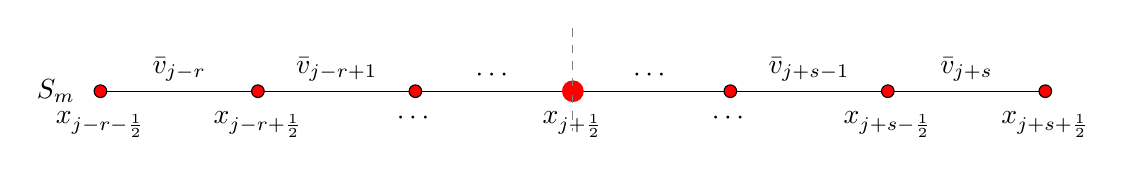
\begin{tikzpicture}[>=stealth]

    % 参数：r=2, s=1 为示例（共 n+1=4 个节点，对应 n=3）
    % 节点位置：x_{j-r-1/2} 到 x_{j+s+1/2}
    % 对应界面：j-5/2, j-3/2, j-1/2, j+1/2, j+3/2
    % 对应单元均值：j-2, j-1, j, j+1

    % ---------- 单元均值标注（上方）----------
    \node[above] at (1,  0) {$\bar{v}_{j-r}$};
    \node[above] at (3,  0) {$\bar{v}_{j-r+1}$};
    \node[above] at (5,  0) {$\cdots$};
    \node[above] at (7,  0) {$\cdots$};
    \node[above] at (9,  0) {$\bar{v}_{j+s-1}$};
    \node[above] at (11,  0) {$\bar{v}_{j+s}$};

    % ---------- 主数轴 ----------
    \draw (0,0) -- (12,0);

    % ---------- 全局模板 S_m 的界面节点（红色）----------
    \foreach \x/\lbl in {
        0/{$x_{j-r-\frac{1}{2}}$},
        2/{$x_{j-r+\frac{1}{2}}$},
        4/{},
        6/{$x_{j+\frac{1}{2}}$},
        8/{},
        10/{$x_{j+s-\frac{1}{2}}$},
        12/{$x_{j+s+\frac{1}{2}}$}
    }{
        \draw[fill=red] (\x,0) circle (0.08) node[below=4pt] {\lbl};
    }

    % 省略号位置补充标注
    \node[below=4pt] at (4,0) {$\cdots$};
    \node[below=4pt] at (8,0) {$\cdots$};

    % 目标界面 x_{j+1/2} 加粗标记
    \draw[fill=red, draw=red, line width=1pt] (6,0) circle (0.12);

    % S_m 标签
    \node[left] at (-0.2, 0) {$S_m$};

    % ---------- 目标界面竖线 ----------
    \draw[dashed, gray] (6, 0.8) -- (6, -0.5);
    % \node[above, gray] at (6, 0.8) {\footnotesize 目标界面};

    % % ---------- 模板范围括号（下方）----------
    % \draw[decorate, decoration={brace, amplitude=6pt, mirror}]
    %     (0, -0.9) -- (10, -0.9)
    %     node[midway, below=8pt] {$n+1$ 个插值节点};

    % % ---------- 左侧 r 段标注 ----------
    % \draw[<->, blue] (0, -1.6) -- (6, -1.6)
    %     node[midway, below=3pt, blue] {$r+1$ 个节点（左侧）};

    % % ---------- 右侧 s 段标注 ----------
    % \draw[<->, teal] (6, -1.6) -- (10, -1.6)
    %     node[midway, below=3pt, teal] {$s$ 个节点（右侧）};

\end{tikzpicture}

% %         \caption{基于原函数的重构示意图：通过对原函数 $H(x)$ 进行插值并求导，得到界面处的重构值}
% %         \label{fig:recon}
% %     \end{figure}


% %     \subsection{非多项式函数重构方法}

% %     设计算域被划分为均匀网格，单元 $I_j = [x_{j-1/2}, x_{j+1/2}]$，
% %     网格间距为 $h$。给定函数 $v(x)$ 在模板
% %     \begin{equation}
% %         S^n(j) = \{I_{j-r}, I_{j-r+1}, \ldots, I_{j+s}\}
% %     \end{equation}
% %     上各单元的平均值
% %     \begin{equation}
% %         \bar{v}_i = \frac{1}{h}\int_{I_i} v(\xi)\,\mathrm{d}\xi,
% %         \quad I_i \in S^n(j),
% %     \end{equation}
% %     其中 $n = r + s + 1$，目标是在 $n$ 维函数空间 $\Omega_n$ 中
% %     找到一个重构函数 $\hat{v}(x)$ 来逼近 $v(x)$。
    
% %     对于传统 WENO 格式，$\Omega_n$ 取为 $n-1$ 次多项式空间。
% %     本文考虑更一般的带形状参数 $\lambda$ 的非多项式函数空间：
% %     \begin{equation}
% %         \Omega_n(x, j, \lambda)
% %         = \mathrm{span}\bigl\{
% %         \varphi_0(x - x_j;\, \lambda),\;
% %         \varphi_1(x - x_j;\, \lambda),\;
% %         \ldots,\;
% %         \varphi_{n-1}(x - x_j;\, \lambda)
% %         \bigr\} \subset C^\infty(\mathbb{R}).
% %     \end{equation}
    
    
    
    
    
% %     \paragraph{重构函数的构造方法}
% %     \textbf{方法一：基于守恒性质的积分重构}
    
% %     该方法基于积分守恒约束。对于模板 $S(j)$ 中的每个单元 $I_i = [x_{i-1/2}, x_{i+1/2}]$（宽度为 $h$），要求重构函数 $\hat{v}(x)$ 满足
% %     \begin{equation}
% %         \label{eq:integral_conservation}
% %         \int_{I_i} \hat{v}(x)\,\mathrm{d}x = \bar{v}_i\,h, \qquad \forall\, I_i \in S(j).
% %     \end{equation}
% %     设重构函数 $\hat{v}(x)$ 属于一维有限维函数空间
% %     $\Omega_n = \mathrm{span}\{\varphi_0(x), \ldots, \varphi_{n-1}(x)\}$，
% %     并将其展开为
% %     \begin{equation}
% %         \hat{v}(x) = \sum_{k=0}^{n-1} c_k\,\varphi_k(x).
% %     \end{equation}
% %     将上式代入守恒条件~\eqref{eq:integral_conservation}，对模板中每个单元逐一列方程，得线性方程组
% %     \begin{equation}
% %         \sum_{k=0}^{n-1} c_k \int_{I_i} \varphi_k(x)\,\mathrm{d}x = \bar{v}_i\,h.
% %     \end{equation}
% %     引入矩阵与向量记号
% %     \begin{equation}
% %         \bm{A}_{ik} = \int_{I_i} \varphi_k(x)\,\mathrm{d}x, \qquad
% %         \bm{c} = \begin{pmatrix} c_0 \\ \vdots \\ c_{n-1} \end{pmatrix}, \qquad
% %         \bm{b} = \begin{pmatrix} \bar{v}_i\,h \\ \vdots \\ \bar{v}_{i+n-1}\,h \end{pmatrix},
% %     \end{equation}
% %     则上述方程组等价于线性系统
% %     \begin{equation}
% %         \bm{A}\,\bm{c} = \bm{b}.
% %     \end{equation}
% %     当矩阵 $\bm{A}$ 可逆时，系数向量 $\bm{c}$ 唯一确定，从而重构函数 $\hat{v}(x)$ 唯一确定。$\bm{A}$ 可逆的充要条件为：各基函数在对应单元上的积分所构成的列向量线性无关，即矩阵 $\bm{A}$ 非奇异。
    
% %     \textbf{方法二} 该方法的核心思路是：先对被重构函数构造原函数，再对原函数的插值多项式求导，从而得到所需的重构函数。设 $v(x)$ 的一个原函数为
% %     \begin{equation}
% %         H(x) = \int_{-\infty}^{x} v(t)\,\mathrm{d}t,
% %     \end{equation}
% %     则对第 $i$ 个单元而言，其两端界面处满足
% %     \begin{equation}
% %         H(x_{i+1/2}) - H(x_{i-1/2}) = \int_{I_i} v(x)\,\mathrm{d}x = \bar{v}_i\,h.
% %     \end{equation}
% %     因此，以某参考界面 $x_{p-1/2}$ 为起点，通过逐单元累加可得
% %     \begin{equation}
% %         H(x_{j+1/2}) = H(x_{p-1/2}) + h\sum_{i=p}^{j} \bar{v}_i.
% %     \end{equation}
% %     注意到常数 $H(x_{p-1/2})$ 在后续求导中不产生影响，故可忽略。
    
% %     \begin{figure}[!htbp]
% %         \centering
% %         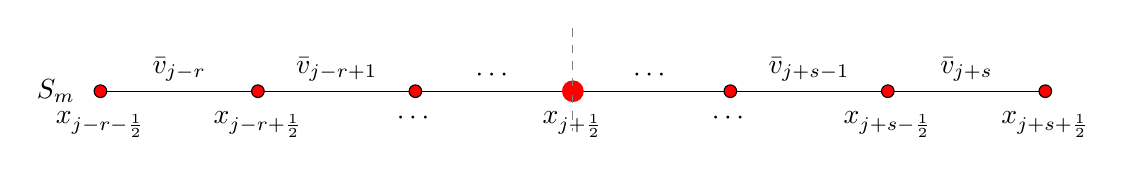
\begin{tikzpicture}[>=stealth]

    % 参数：r=2, s=1 为示例（共 n+1=4 个节点，对应 n=3）
    % 节点位置：x_{j-r-1/2} 到 x_{j+s+1/2}
    % 对应界面：j-5/2, j-3/2, j-1/2, j+1/2, j+3/2
    % 对应单元均值：j-2, j-1, j, j+1

    % ---------- 单元均值标注（上方）----------
    \node[above] at (1,  0) {$\bar{v}_{j-r}$};
    \node[above] at (3,  0) {$\bar{v}_{j-r+1}$};
    \node[above] at (5,  0) {$\cdots$};
    \node[above] at (7,  0) {$\cdots$};
    \node[above] at (9,  0) {$\bar{v}_{j+s-1}$};
    \node[above] at (11,  0) {$\bar{v}_{j+s}$};

    % ---------- 主数轴 ----------
    \draw (0,0) -- (12,0);

    % ---------- 全局模板 S_m 的界面节点（红色）----------
    \foreach \x/\lbl in {
        0/{$x_{j-r-\frac{1}{2}}$},
        2/{$x_{j-r+\frac{1}{2}}$},
        4/{},
        6/{$x_{j+\frac{1}{2}}$},
        8/{},
        10/{$x_{j+s-\frac{1}{2}}$},
        12/{$x_{j+s+\frac{1}{2}}$}
    }{
        \draw[fill=red] (\x,0) circle (0.08) node[below=4pt] {\lbl};
    }

    % 省略号位置补充标注
    \node[below=4pt] at (4,0) {$\cdots$};
    \node[below=4pt] at (8,0) {$\cdots$};

    % 目标界面 x_{j+1/2} 加粗标记
    \draw[fill=red, draw=red, line width=1pt] (6,0) circle (0.12);

    % S_m 标签
    \node[left] at (-0.2, 0) {$S_m$};

    % ---------- 目标界面竖线 ----------
    \draw[dashed, gray] (6, 0.8) -- (6, -0.5);
    % \node[above, gray] at (6, 0.8) {\footnotesize 目标界面};

    % % ---------- 模板范围括号（下方）----------
    % \draw[decorate, decoration={brace, amplitude=6pt, mirror}]
    %     (0, -0.9) -- (10, -0.9)
    %     node[midway, below=8pt] {$n+1$ 个插值节点};

    % % ---------- 左侧 r 段标注 ----------
    % \draw[<->, blue] (0, -1.6) -- (6, -1.6)
    %     node[midway, below=3pt, blue] {$r+1$ 个节点（左侧）};

    % % ---------- 右侧 s 段标注 ----------
    % \draw[<->, teal] (6, -1.6) -- (10, -1.6)
    %     node[midway, below=3pt, teal] {$s$ 个节点（右侧）};

\end{tikzpicture}

% %         \caption{}
% %         \label{fig:recon}
% %     \end{figure}
    
% %     在插值节点集
% %     \begin{equation}
% %         S_m = \bigl\{x_{j-r-1/2},\, x_{j-r+1/2},\, \ldots,\, x_{j+s+1/2}\bigr\}
% %     \end{equation}
% %     上，构造 $H$ 的 $n+1$ 阶拉格朗日插值多项式
% %     \begin{equation}
% %         H_{n+1}(x) = \sum_{m=0}^{n} H\!\left(x_{j-r+m-1/2}\right) L_m(x),
% %     \end{equation}
% %     其中 $L_m(x)$ 为满足插值条件
% %     \begin{equation}
% %         L_m\!\left(x_{j-r+k-1/2}\right) = \delta_{mk}, \quad k = 0,1, \ldots, n
% %     \end{equation}
% %     的拉格朗日基函数。要求 $L_m'(x) \in \Omega_n$，从而使得重构函数
% %     \begin{equation}
% %         \hat{v}(x) := H_{n+1}'(x) \in \Omega_n.
% %     \end{equation}
% %     于是，界面 $x_{j+1/2}$ 处的重构值为
% %     \begin{equation}
% %         \hat{v}_{j+1/2} = H_{n+1}'\!\left(x_{j+1/2}\right)
% %         = \sum_{m=0}^{n} H\!\left(x_{j-r+m-1/2}\right) L_m'\!\left(x_{j+1/2}\right).
% %     \end{equation}
    
% %     为确定满足上述条件的拉格朗日基函数，记 
% %     \begin{equation}
% %         \phi_0(x) = 1,\, \phi_k(x) = \int_{-\infty}^x\varphi_{k-1}(t),\quad k = 1, 2, \ldots, n
% %     \end{equation}
% %     要求基函数满足如下插值条件：
% %     \begin{equation}
% %         \sum_{k=0}^{n} L_k(x)\,\phi_\ell\!\left(x_{j-r+k-1/2}\right) = \phi_\ell(x),
% %         \quad \ell = 0, \ldots, n.
% %     \end{equation}
% %     引入矩阵与向量记号
% %     \begin{equation}
% %         \bm{A} = \begin{bmatrix}
% %             \phi_0(x_{j-r-1/2}) & \phi_0(x_{j-r+1/2}) & \cdots & \phi_0(x_{j+s+1/2}) \\
% %             \phi_1(x_{j-r-1/2}) & \phi_1(x_{j-r+1/2}) & \cdots & \phi_1(x_{j+s+1/2}) \\
% %             \vdots & \vdots & \ddots & \vdots \\
% %             \phi_{n}(x_{j-r-1/2}) & \phi_{n}(x_{j-r+1/2}) & \cdots & \phi_{n}(x_{j+s+1/2}) \\
% %         \end{bmatrix}, \quad
% %         \bm{L}(x) = \begin{pmatrix} L_0(x) \\ \vdots \\ L_n(x) \end{pmatrix}, \quad
% %         \bm{b}(x) = \begin{pmatrix} \phi_0(x) \\ \vdots \\ \phi_n(x) \end{pmatrix},
% %     \end{equation}
% %     则上述条件等价于线性方程组
% %     \begin{equation}
% %         \bm{A}\,\bm{L}(x) = \bm{b}(x).
% %     \end{equation}
% %     当矩阵 $\bm{A}$ 可逆时，拉格朗日基函数 $\{L_k(x)\}_{k=0}^{n}$ 唯一确定，从而完成重构。
% %     \begin{remark}
% %         方法二中矩阵 $\bm{A}$ 的奇异性等价于方法一中如下 $n \times n$ 矩阵
% %         \begin{equation}
% %             \bm{B} = 
% %             \begin{bmatrix}
% %                 \int_{I_{j-r}} \varphi_0(x)\,\mathrm{d}x & \int_{I_{j-r+1}} \varphi_0(x)\,\mathrm{d}x & \cdots & \int_{I_{j+s}} \varphi_0(x)\,\mathrm{d}x \\
% %                 \int_{I_{j-r}} \varphi_1(x)\,\mathrm{d}x & \int_{I_{j-r+1}} \varphi_1(x)\,\mathrm{d}x & \cdots & \int_{I_{j+s}} \varphi_1(x)\,\mathrm{d}x \\
% %                 \vdots & \vdots & \ddots & \vdots \\
% %                 \int_{I_{j-r}} \varphi_{n-1}(x)\,\mathrm{d}x & \int_{I_{j-r+1}} \varphi_{n-1}(x)\,\mathrm{d}x & \cdots & \int_{I_{j+s}} \varphi_{n-1}(x)\,\mathrm{d}x
% %             \end{bmatrix}
% %         \end{equation}
% %         的奇异性。
% %     \end{remark}
% %     \subsection{非多项式基函数}

% % 为构造具有高精度与良好数值性质的非多项式重构，需要对逼近空间 $\Omega_n$ 施加适当约束。下面给出构造非多项式基函数时所需满足的基本性质。

% % \begin{property}[包含常数]
% % 空间 $\Omega_n$ 必须包含常数函数，即
% % \[
% % 1 \in \Omega_n.
% % \]
% % 该性质保证重构能够精确再现常数解，从而维持守恒性。
% % \end{property}

% % \begin{property}[对称性]
% % 若 $\varphi_k(x;\lambda) \in \Omega_n$，则有
% % \[
% % \varphi_k(-x;\lambda) \in \Omega_n.
% % \]
% % 该性质用于保证重构在对称模板下具有一致性，从而避免引入非物理偏差。
% % \end{property}

% % \begin{property}[渐近多项式再现性]
% % 对于任意 $\ell = 0,1,\ldots,n-1$，存在系数向量 $\bm{c}_\ell(\lambda)$，使得
% % \begin{equation}
% % x^\ell = \sum_{i=0}^{n-1} c_{\ell,i}(\lambda)\,\varphi_i(x;\lambda) + \mathcal{O}(\lambda h^n), \quad \lambda \to 0.
% % \end{equation}
% % 该性质表明，当 $\lambda \to 0$ 时，非多项式空间可渐近退化为多项式空间，从而保证高阶精度。
% % \end{property}

% % \begin{property}[积分矩阵可逆性]
% % 定义积分矩阵
% % \begin{equation}
% % \bm{A}_{i,k} = \int_{I_i} \varphi_k(x)\,\mathrm{d}x,
% % \end{equation}
% % 要求矩阵 $\bm{A}$ 非奇异。
% % 该条件保证重构问题具有唯一解。
% % \end{property}

% % 在上述条件下，基于 $\Omega_n$ 构造的重构函数具有以下性质。

% % \begin{theorem}[常数保持性]
% % 若 $v(x)$ 为常数函数，则其重构函数 $\hat{v}(x)$ 亦为常数函数。
% % \end{theorem}

% % \begin{proof}
% % 当 $v(x) \equiv C$ 时，单元平均值满足 $\bar{v}_i = C$。由于 $1 \in \Omega_n$，常数函数属于逼近空间。由重构问题的唯一性可知，$\hat{v}(x)$ 必为常数函数。
% % \end{proof}

% % \begin{theorem}[对称性]
% % \label{thm:nonpol_symmetry}
% % 考虑两个对称模板
% % \begin{equation}
% % \begin{aligned}
% % S^L &= \{I_{j-r}, \ldots, I_{j+s}\},\\
% % S^R &= \{I_{\tilde{j}-s}, \ldots, I_{\tilde{j}+r}\},
% % \end{aligned}
% % \end{equation}
% % 若满足
% % \begin{equation}
% % \bar{v}_{j-k} = \bar{v}_{\tilde{j}+k}, \quad k = -s,\ldots,r,
% % \end{equation}
% % 则对应的重构函数满足
% % \begin{equation}
% % \hat{v}^L(x) = \hat{v}^R(-x + x_j + x_{\tilde{j}}).
% % \end{equation}
% % 特别地，在界面处有
% % \begin{equation}
% % \hat{v}^L(x_{j+1/2}) = \hat{v}^R(x_{\tilde{j}-1/2}).
% % \end{equation}
% % \end{theorem}

% % \begin{proof}
% % 构造函数
% % \[
% % w(x) = \hat{v}^L(-x + x_j + x_{\tilde{j}}),
% % \]
% % 利用变量替换可验证 $w(x)$ 满足模板 $S^R$ 上的所有积分守恒条件。由重构解的唯一性可知 $w(x)=\hat{v}^R(x)$，从而得到结论。
% % \end{proof}

% % \begin{theorem}[高阶精度]
% % \label{thm:nonpol_accuracy}
% % 基于 $\Omega_n$ 的重构在单元界面处满足
% % \begin{equation}
% % v(x_{j+1/2}) - \hat{v}(x_{j+1/2}) = \mathcal{O}(h^n).
% % \end{equation}
% % \end{theorem}

% % \begin{proof}
% % 由渐近多项式再现性，可构造一组等价基函数，使其在 $\lambda \to 0$ 时逼近多项式基。利用重构问题的唯一性，该重构与多项式重构在主导项上一致。结合多项式 WENO 重构的 $n$ 阶精度性质，即可得到结论。
% % \end{proof}

% % \begin{remark}
% % 例如，当
% % \begin{equation}
% % \Omega_5 = \mathrm{span}\{1, x, x^2, e^{-\lambda x}, e^{\lambda x}\},
% % \end{equation}
% % 通过泰勒展开可验证指数函数在 $\lambda \to 0$ 时可表示为多项式的高阶扰动，从而满足渐近多项式再现性。
% % \end{remark}
% % \subsection{非多项式基函数}

% % 为构造具有高精度与良好数值性质的非多项式重构格式，需对逼近空间 $\Omega_n$ 施加适当约束。
% % 本节给出构造非多项式基函数所需满足的基本性质，并在此基础上建立相应的理论结果。
% % \begin{property}[积分矩阵可逆性]
% %     定义积分矩阵
% %     \begin{equation}
% %     \bm{A}_{i,k} = \int_{I_i} \varphi_k(x)\,\mathrm{d}x,
% %     \end{equation}
% %     要求矩阵 $\bm{A}$ 非奇异。该条件保证重构问题存在唯一解。
% %     \end{property}
    
% % \begin{property}[包含常数]
% % 空间 $\Omega_n$ 必须包含常数函数，即
% % \[
% % 1 \in \Omega_n.
% % \]
% % 该性质保证重构格式能够精确再现常数解，从而维持数值守恒性。
% % \end{property}

% % \begin{property}[对称性]
% % 若 $\varphi_k(x) \in \Omega_n$，则有
% % \[
% % \varphi_k(2x_j - x;\lambda) \in \Omega_n(x, j, \lambda).
% % \]
% % 该性质保证在对称模板下重构结果相等。
% % \end{property}

% % \begin{property}[渐近多项式再现性]
% % 对任意 $\ell = 0,1,\ldots,n-1$，存在系数向量 $\bm{c}_\ell(\lambda)$，使得
% % \begin{equation}
% % x^\ell = \sum_{i=0}^{n-1} c_{\ell,i}(\lambda)\,\varphi_i(x;\lambda) + \mathcal{O}(\lambda h^n),
% % \quad \lambda \to 0.
% % \end{equation}
% % 该性质表明，当 $\lambda \to 0$ 时，非多项式逼近空间可渐近退化为相应的多项式空间。
% % \end{property}


% % 基于上述四条性质，可在空间 $\Omega_n$ 中建立以下理论结果。

% % \begin{theorem}[常数保持性]
% % 若 $v(x)$ 为常数函数，则其重构函数 $\hat{v}(x)$ 亦为常数函数。
% % \end{theorem}

% % \begin{proof}
% % 设 $v(x) \equiv C$，则各单元平均值满足 $\bar{v}_i = C$。
% % 由性质~2，常数函数属于逼近空间 $\Omega_n$，故 $\hat{v}(x) \equiv C$ 是重构问题的一个解。再由性质~1 保证的重构唯一性，结论成立。
% % \end{proof}

% % \begin{theorem}[对称性]
% % \label{thm:nonpol_symmetry}
% % 考虑两个对称模板
% % \begin{equation}
% % \begin{aligned}
% % S^L &= \{I_{j-r}, \ldots, I_{j+s}\},\\
% % S^R &= \{I_{\tilde{j}-s}, \ldots, I_{\tilde{j}+r}\}.
% % \end{aligned}
% % \end{equation}
% % 若满足
% % \begin{equation}
% % \bar{v}_{j-k} = \bar{v}_{\tilde{j}+k}, \quad k = -s,\ldots,r,
% % \end{equation}
% % 则对应的重构函数满足
% % \begin{equation}
% % \hat{v}^L(x) = \hat{v}^R(-x + x_j + x_{\tilde{j}}).
% % \end{equation}
% % 特别地，在单元界面处有
% % \begin{equation}
% % \hat{v}^L(x_{j+1/2}) = \hat{v}^R(x_{\tilde{j}-1/2}).
% % \end{equation}
% % \end{theorem}

% % \begin{proof}
% % 构造辅助函数
% % \[
% % w(x) = \hat{v}^L(-x + x_j + x_{\tilde{j}}).
% % \]
% % 由变量替换及模板对称条件，可验证 $w(x)$ 满足模板 $S^R$ 上的所有积分守恒约束。再由性质~1 保证的重构唯一性，得 $w(x) = \hat{v}^R(x)$，结论成立。
% % \end{proof}

% % \begin{theorem}[高阶精度]
% % \label{thm:nonpol_accuracy}
% % 基于 $\Omega_n$ 的重构在单元界面处满足
% % \begin{equation}
% % v(x_{j+1/2}) - \hat{v}(x_{j+1/2}) = \mathcal{O}(h^n).
% % \end{equation}
% % \end{theorem}

% % \begin{proof}
% % 由性质~3（渐近多项式再现性），当 $\lambda \to 0$ 时，空间 $\Omega_n$ 中的基函数可
% % 展开为多项式基函数的高阶扰动，从而可构造一组在主导项上与多项式基等价的基函数。
% % 在此基础上，利用性质~4 保证的重构唯一性，
% % 基于 $\Omega_n$ 的重构函数在主导截断误差项上与经典多项式重构一致。
% % 结合多项式 WENO 格式的 $n$ 阶精度结论，即得所证不等式成立。
% % \end{proof}

% % \begin{remark}
% % 以五点逼近空间为例，取
% % \begin{equation}
% % \Omega_5 = \mathrm{span}\{1, x, x^2, e^{-\lambda x}, e^{\lambda x}\}.
% % \end{equation}
% % 对指数函数作 Taylor 展开，可知 $e^{\pm\lambda x}$ 在 $\lambda \to 0$
% % 时退化为多项式的高阶扰动，从而验证性质~3 对该空间成立。
% % \end{remark}


% % \subsection{边界条件}

% % 本文所涉及的边界条件通过虚拟单元（ghost cell）方法实现，
% % 即在计算域边界外设置一层虚拟单元，并按如下规则赋值。

% % \paragraph{自由流入边界条件}
% % 在入口边界处，将给定的来流状态直接赋予虚拟单元：
% % \begin{equation}
% %     \bm{Q}_{\mathrm{ghost}} = \bm{Q}_{\infty},
% % \end{equation}
% % 其中 $\bm{Q}_\infty$ 为指定的来流守恒变量。

% % \paragraph{自由流出边界条件}
% % 在出口边界处，采用零梯度（无反射）条件，
% % 即将边界内侧单元的状态直接复制至虚拟单元：
% % \begin{equation}
% %     \bm{Q}_{\mathrm{ghost}} = \bm{Q}_{\mathrm{interior}},
% % \end{equation}
% % 该条件等价于 $\partial \bm{Q}/\partial n = 0$，
% % 适用于超声速出口或弱反射情形。

% % \paragraph{固壁反射边界条件}
% % 对于无粘流动，固壁处采用滑移边界条件，
% % 物理要求为法向速度为零，切向速度不受约束。
% % 通过对虚拟单元施加镜像处理来实现：
% % \begin{equation}
% %     \bm{u}_{\mathrm{ghost}}
% %     = \bm{u}_{\mathrm{interior}}
% %     - 2(\bm{u}_{\mathrm{interior}} \cdot \bm{n})\,\bm{n},
% % \end{equation}
% % 其余状态量（密度、压力）与内侧单元保持一致：
% % \begin{equation}
% %     (\tilde{\rho}_k)_{\mathrm{ghost}} = (\tilde{\rho}_k)_{\mathrm{interior}},
% %     \quad k = 1, 2.
% % \end{equation}
% % 该处理方式使得界面处法向速度严格为零，
% % 即 $\bm{u} \cdot \bm{n} \big|_{\mathrm{wall}} = 0$，
% % 同时切向速度保持不变，符合无粘欧拉方程的物理约束。

% % \subsection{指数多项式逼近空间 WENO 格式}
% % 本文选取如下的非多项式基函数，
% % \begin{equation}
% %     \Omega_3 = \mathrm{span}\bigl\{1,\; \tanh(\lambda x), \; x^2\; \bigr\},
% %     \qquad
% %     \Omega_5 = \mathrm{span}\bigl\{1,\; x,\; x^2,\; \tanh(\lambda x),\; x^4\bigr\}.
% % \end{equation}
% % 这一选择满足性质~1--4 的全部要求。

% % 利用 Taylor 展开，大模板重构值 $\hat{v}_{j+1/2}$ 
% % 关于精确解的截断误差可表示为
% % \begin{equation}
% %     \label{eq:exp1_accuracy}
% %     \hat{v}_{j+1/2}
% %     = v(x_{j+1/2})
% %     + \left(\frac{v^{(4)} \lambda^2}{15} + \frac{v^{(6)}}{140}\right)h^6
% %     + \left(-\frac{2v^{(3)}\lambda^2}{15} - \frac{v^{(5)}}{60}\right)h^5
% %     + \mathcal{O}(h^7).
% % \end{equation}
% % 由式~\eqref{eq:exp1_accuracy} 可知，当
% % \begin{equation}
% %     \label{eq:l2h2_condition}
% %     \lambda^2  = -\frac{1}{8}\frac{v^{(5)}(x_{j+1/2})}{v^{(3)}(x_{j+1/2})} + \mathcal{O}(h),
% % \end{equation}
% % 时，式~\eqref{eq:exp1_accuracy}中的 $h^5$ 项消失，
% % WENO-EXP 格式的大模板重构精度从五阶提升至六阶。

% % 在实际计算中，本文通过如下公式计算形状参数 $\lambda$：
% % \begin{equation}
% % \lambda^2 := \Delta x^{-2} \frac{\mathbb{D}^5 u_{j+\frac{1}{2}}}{\mathbb{D}^3 u_{j+\frac{1}{2}}},
% % \end{equation}
% % 其中，算子 $\mathbb{D}^m u$ 表示 $u$ 的一种广义未除差分（generalized undivided difference），
% % 用于近似 $\Delta x^m u^{(m)}$。

% % 可以证明
% % \begin{equation}
% %     \begin{aligned}
% %     \mathbb{D}^3 u_{j+1/2} &\coloneqq \frac{\bar{u}_{j-2} - 11\bar{u}_{j-1} + 28\bar{u}_j - 28\bar{u}_{j+1} + 11\bar{u}_{j+2} - \bar{u}_{j+3}}{6}\\ 
% %     &=u^{(3)}h^3 + \mathbb{O}(h^7),\\
% %     \mathbb{D}^5 u_{j+1/2} &\coloneqq -\bar{u}_{j-2} + 5\bar{u}_{j-1} - 10\bar{u}_j + 10\bar{u}_{j+1} - 5\bar{u}_{j+2} + \bar{u}_{j+3} \\ 
% %     &= u^{(5)}h^5 + \mathbb{O}(h^7),
% % \end{aligned}
% % \end{equation}



% % 由三点子模板 $\{I_{j-2}, I_{j-1}, I_j\}$、$\{I_{j-1}, I_j, I_{j+1}\}$、$\{I_j, I_{j+1}, I_{j+2}\}$在函数空间 $\Omega_3$ 中分别进行重构，所得三个候选重构值为（以形状参数 $\lambda$ 的幂次展开，令 $\ell = \lambda^2 h^2$）：
% % \begin{equation}
% %     \label{eq:exp_substencil}
% %     \begin{aligned}
% %         \hat{v}^0_{j+1/2}
% %         = & \left(\frac{11}{6}\bar{u}_j - \frac{7}{6}\bar{u}_{j-1}
% %         + \frac{1}{3}\bar{u}_{j-2}\right)
% %         + \left(-\frac{3}{4}\bar{u}_j + \bar{u}_{j-1}
% %         - \frac{1}{4}\bar{u}_{j-2}\right)\ell \\
% %           & + \left(\frac{207}{80}\bar{u}_j - \frac{69}{20}\bar{u}_{j-1}
% %         + \frac{69}{80}\bar{u}_{j-2}\right)\ell^2, \\[6pt]
% %         \hat{v}^1_{j+1/2}
% %         = & \left(\frac{5}{6}\bar{u}_j - \frac{1}{6}\bar{u}_{j-1}
% %         + \frac{1}{3}\bar{u}_{j+1}\right)
% %         + \left(-\frac{1}{12}\bar{u}_{j-1}
% %         + \frac{1}{12}\bar{u}_{j+1}\right)\ell \\
% %           & + \left(\frac{19}{720}\bar{u}_{j-1}
% %         - \frac{19}{720}\bar{u}_{j+1}\right)\ell^2, \\[6pt]
% %         \hat{v}^2_{j+1/2}
% %         = & \left(\frac{1}{3}\bar{u}_j + \frac{5}{6}\bar{u}_{j+1}
% %         - \frac{1}{6}\bar{u}_{j+2}\right)
% %         + \left(\frac{1}{4}\bar{u}_j - \frac{1}{3}\bar{u}_{j+1}
% %         + \frac{1}{12}\bar{u}_{j+2}\right)\ell \\
% %           & + \left(-\frac{271}{240}\bar{u}_j + \frac{271}{180}\bar{u}_{j+1}
% %         - \frac{271}{720}\bar{u}_{j+2}\right)\ell^2.
% %     \end{aligned}
% % \end{equation}
% % 当 $\ell = 0$ 时，式~\eqref{eq:exp_substencil} 退化为
% % WENO-JS 的三点多项式重构公式，与定理~\autoref{thm:nonpol_accuracy}
% % 的渐近退化性质一致。

% % 由大模板重构的线性组合条件确定的最优线性权重为：
% % \begin{equation}
% %     \label{eq:exp_linear_weights}
% %     \begin{aligned}
% %         d_0 & = \frac{1}{10} + \frac{11}{40}\ell - \frac{1111}{8400}\ell^2,\\
% %         d_1 & = \frac{3}{5}  - \frac{33}{40}\ell +\frac{243}{350}\ell^2,\\
% %         d_2 & = \frac{3}{10} + \frac{11}{20}\ell - \frac{4721}{8400}\ell^2.
% %     \end{aligned}
% % \end{equation}
% % 当 $\ell = 0$ 时，线性权重~\eqref{eq:exp_linear_weights}退化为 WENO-JS 的最优权重。

% % \begin{figure}[!htbp]
% %     \centering
% %     \begin{subfigure}[t]{0.45\linewidth}
% %         \centering
% %         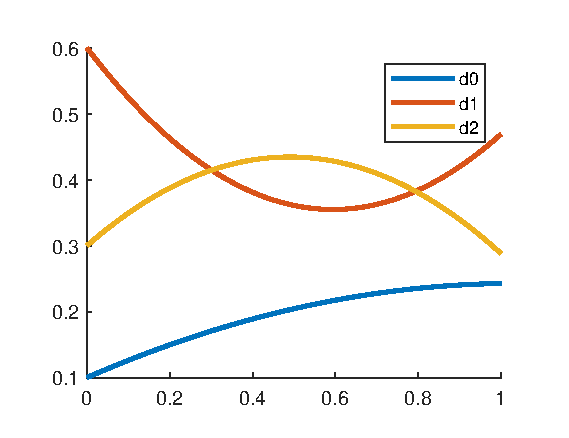
\includegraphics[width=\linewidth]{figure/other/d0d1d1_right.eps}
% %         \caption{}
% %     \end{subfigure}
% %     \hfill
% %     \begin{subfigure}[t]{0.45\linewidth}
% %         \centering
% %         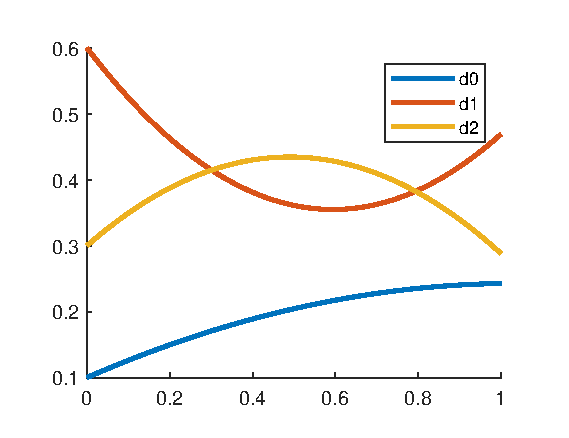
\includegraphics[width=\linewidth]{figure/other/d0d1d1_right.eps}
% %         \caption{}
% %     \end{subfigure}
% %     \caption{}
% %     \label{fig:}
% % \end{figure}

% % % \begin{remark}
% % %     可以验证，对于任意 $\ell$，三个线性权重之和恒为
% % %     $d_0 + d_1 + d_2 = 1$，这是 WENO 格式的基本一致性条件。%此外，为保证线性权重均为非负，$\ell$ 须满足一定的上界约束，该约束来自 $d_1 \geqslant 0$ 的条件，详见第~X节关于形状参数上界的讨论。
% % % \end{remark}
% % % 可以证明，$d-\alpha_k$

% % 与基于多项式逼近的传统 WENO 重构类似，为抑制间断附近的非物理振荡，引入非线性权重。为了在光滑区域达到六阶精度，只需非线性权重 $\gamma_\ell$ 满足
% % \begin{equation}
% %     \gamma_\ell - d_\ell = \mathcal{O}(\Delta x^4).
% % \end{equation}
% % 在本文中，非线性权重定义为
% % \begin{equation}
% % \gamma_\ell = \frac{\nu_\ell}{\sum_{\ell=0}^{2} \nu_\ell}, 
% % \qquad
% % \nu_\ell = d_\ell \left( 1 + \frac{\tau_5^2}{\beta_\ell^2 + \varepsilon} \right),
% % \end{equation}
% % 其中 $\varepsilon$ 为防止分母为零而引入的一个小正数。局部与全局光滑性指标，即 $\beta_\ell$ 和 $\tau_5$，定义为
% % \begin{equation}
% % \beta_\ell(\bar{u}_{j-2+\ell}, \bar{u}_{j-1+\ell}, \bar{u}_{j+\ell})
% % = \left| \mathbb{D}^1 u_j^{[\ell]} \right|
% % + \left| \mathbb{D}^2 u_j^{[\ell]} \right|,
% % \qquad
% % \tau_5 = \left| \mathbb{D}^4 u_j \right|.
% % \end{equation}
% % 即：
% % \begin{equation}
% %     \label{eq:beta_improved}
% %     \begin{aligned}
% %         \beta_0 & = \frac{1}{2}|\bar{u}_{j-2} - 4\bar{u}_{j-1} + 3\bar{u}_j|
% %         + |\bar{u}_{j-2} - 2\bar{u}_{j-1} + \bar{u}_j|,             \\
% %         \beta_1 & = \frac{1}{2}|\bar{u}_{j-1} - \bar{u}_{j+1}|
% %         + |\bar{u}_{j-1} - 2\bar{u}_j + \bar{u}_{j+1}|,              \\
% %         \beta_2 & = \frac{1}{2}|3\bar{u}_j - 4\bar{u}_{j+1} + \bar{u}_{j+2}|
% %         + |\bar{u}_j - 2\bar{u}_{j+1} + \bar{u}_{j+2}|,\\ 
% %         \tau & = \bar{u}_{j-2} - 4\bar{u}_{j-1}
% %           + 6\bar{u}_j - 4\bar{u}_{j+1} + \bar{u}_{j+2}
% %     \end{aligned}
% % \end{equation}
% % 有此可得以下定理
% % \begin{lemma}
% %     若取 $\varepsilon = \mathcal{O}(\Delta x^4)$，则式(28)定义的非线性权重满足条件(27)，即使在临界点 $u'(x_j)=0$ 附近亦成立。
% % \end{lemma}
% % \begin{proof}
% %     对 $\beta_\ell$ 和 $\tau_5$ 在 $x_j$ 处作 Taylor 展开，有
% % \begin{align}
% % \beta_\ell &= \left| u'(x_j)\Delta x \right|
% % + \left| u''(x_j)\Delta x^2 \right|
% % + \mathcal{O}(\Delta x^3), \\
% % \tau_5 &= \left| u^{(4)}(x_j)\Delta x^4 \right|
% % + \mathcal{O}(\Delta x^5).
% % \end{align}

% % 考虑如下两种情况：
% % \begin{itemize}
% % \item \textbf{情况 1：} $u'(x_j) \neq 0$。此时 $\beta_\ell = \mathcal{O}(\Delta x)$，从而
% % \[
% % \frac{\tau_5^2}{\beta_\ell^2 + \varepsilon} = \mathcal{O}(\Delta x^6).
% % \]

% % \item \textbf{情况 2：} $u'(x_j) = 0$。此时 $\beta_\ell = \mathcal{O}(\Delta x^2)$，从而
% % \[
% % \frac{\tau_5^2}{\beta_\ell^2 + \varepsilon} = \mathcal{O}(\Delta x^4).
% % \]
% % \end{itemize}

% % 因此，有 $\nu_\ell - d_\ell = \mathcal{O}(\Delta x^4)$，从而条件(27)成立。
% % \end{proof}


% % \subsection{非多项式基函数}
% % 为使非多项式重构具备高精度与良好的数值性质，对函数空间 $\Omega_n$ 提出以下约束。

% % \begin{property}[积分矩阵可逆性]
% %     \label{prop:nonpol_integral_matrix}
% %     定义积分矩阵
% %     \begin{equation}
% %         \bm{A}_{i,k} = \int_{I_i} \varphi_k(x)\,\mathrm{d}x,
% %     \end{equation}
% %     要求矩阵 $\bm{A}$ 非奇异。
% % \end{property}

% % \begin{property}[包含常数]
% %     \label{prop:nonpol_const}
% %     空间 $\Omega_n$ 必须包含常数函数：$1 \in \Omega_n$。
% % \end{property}

% % \begin{property}[对称性]
% %     \label{prop:nonpol_symmetry}
% %     若 $\varphi_k(x;\lambda) \in \Omega_n$，则 $\varphi_k(-x+2x_j;\lambda) \in \Omega_n$。
% % \end{property}

% % \begin{property}[渐近多项式再现性]
% %     \label{prop:nonpol_asymp_poly}
% %     存在系数向量 $\bm{c}_\ell(\lambda)$，使得对于
% %     $\ell = 0, 1, \ldots, n-1$，一致成立
% %     \begin{equation}
% %         x^\ell - \sum_{i=0}^{n-1} c_{\ell,i}(\lambda)\,\varphi_i(x;\lambda)
% %         = c(\lambda)\mathcal{O}(\Delta x^n), \quad \lambda \to 0.
% %     \end{equation}
% %     其中，$c(\lambda)$ 是 $\lambda$ 的某个函数，满足 $\lim_{\lambda \to 0} c(\lambda) = 0$。
% % \end{property}



% % 基于满足上述要求的函数空间构造的重构函数具有如下的性质：

% % \begin{theorem}
% %     对于常数函数，重构函数也常数函数。这一性质有助于保持质量守恒性以及孤立相界面处的压力与速度均匀性。
% % \end{theorem}
% % \begin{proof}
% %     这个证明是显然的
% % \end{proof}
% % \begin{theorem}[非多项式重构的对称性]
% %     \label{thm:nonpol_symmetry}
% %     对于两个对称的模板 
% %     \begin{equation}
% %         \begin{aligned}
% %             S^L = \{I_{j-r}, I_{j-r+1}, \ldots, I_{j+s}\}\\ 
% %             S^R = \{I_{\tilde{j}-s}, I_{\tilde{j}-s+1}, \ldots, I_{\tilde{j}+r}\}\\ 
% %         \end{aligned}
% %     \end{equation}
% %     其中
% %     \begin{equation}
% %         \bar{v}_{j-k} = \bar{v}_{\tilde{j}+k},\quad k =  -s,-s+1,\cdots, r,
% %     \end{equation}
% %     则有
% %     \begin{equation}
% %         \label{eq:nonpol_symmetry}
% %         \hat{v}^{L}(x_j+\Delta x) = \hat{v}^{R}(x_{\tilde{j}}-\Delta x),
% %     \end{equation}
% %     特别的 
% %     \begin{equation}
% %         \label{eq:nonpol_symmetry_interface}
% %         \hat{v}^{L}(x_{j+1/2}) = \hat{v}^{R}(x_{{\tilde{j}}-1/2}).
% %     \end{equation}
% % \end{theorem}

% % \begin{proof}

% %     设模板 $S^L$ 上的重构函数 $\hat{v}^L(x)$ 
% %     % 以 $x_j$ 为中心展开为
% %     % \begin{equation}
% %     %     \hat{v}^L(x) = \sum_{k=0}^{n-1} c_k\,\varphi_k(x - x_j).
% %     % \end{equation}
% %     由数据对称条件 $\bar{v}_{j-k} = \bar{v}_{\tilde{j}+k}$，自然地猜测 $\hat{v}^R(x)$ 具有如下形式
% %     \begin{equation}
% %         w(x) =\hat{v}^L(-x+x_j+x_{\tilde{j}})\in \Omega_n(x,\tilde{j},\lambda),
% %     \end{equation}
% %     令 $\xi = -x+x_j+x_{\tilde{j}}$,且当 $x \in I_{\tilde{j}+k} = [x_{\tilde{j}+k-1/2},\, x_{\tilde{j}+k+1/2}]$ 时，$\xi \in [x_{j-k-1/2}, x_{j-k+1/2}] = I_{j-k}$,其中 $k = -s, \ldots, r$。因此
% %     \begin{equation}
% %         \begin{aligned}
% %             \int_{I_{\tilde{j}+k}} w(x)\,\mathrm{d}x  = & \int_{I_{\tilde{j}+k}} \hat{v}^L(-x+x_j+x_{\tilde{j}})\,\mathrm{d}x \\
% %              = & \int_{I_{j-k}} \hat{v}^L(\xi)\,\mathrm{d} \xi = \bar{v}_{j-k}\,h = \bar{v}_{\tilde{j}+k}\,h.
% %         \end{aligned}
% %     \end{equation}
% %     故 $w(x)$ 满足模板 $S^R$ 上的全部积分守恒条件。由唯一性可知
% %     \begin{equation}
% %         \hat{v}^R(x) = w(x).
% %     \end{equation}
% %     ~\eqref{eq:nonpol_symmetry} 和~\eqref{eq:nonpol_symmetry_interface} 即得证的成立是显然的。
% % \end{proof}


% % \begin{theorem}[非多项式重构的高阶精度]
% %     \label{thm:nonpol_accuracy}
% %     基于 $\Omega_n$ 的重构值在单元界面处满足 $n$ 阶精度：
% %     \begin{equation}
% %         v(x_{j+1/2}) - \hat{v}(x_{j+1/2}) = \mathcal{O}(h^n).
% %     \end{equation}
% %     且重构函数在单元界面处的值在 $\lambda \to 0$ 时退化为多项式重构结果，即：
% %     \begin{equation}
% %         \hat{v}_{j+1/2}^{\mathrm{nonpol}}\xrightarrow{\lambda \to 0}\hat{v}_{j+1/2}^{\mathrm{pol}}.
% %     \end{equation}
% % \end{theorem}
% % \begin{lemma}
% %     使用多项式基函数 $\{p_\ell\}_{\ell=0}^{n-1}$ 重构出的数值通量具有 \(n\) 阶精度.这个在 WENOJS 文献中已经有证明.
% % \end{lemma}
% % \begin{proof}
% %     不妨另外定义一组基函数 $\{\tilde{\varphi}_k(x;\lambda)\}_{k=0}^{n-1}$, 满足
% %     \begin{equation}
% %         \tilde{\varphi}_k(x;\lambda) = \sum_{i=0}^{n-1} c_{\ell,i}(\lambda)\,\varphi_i(x;\lambda) = p_\ell(x) + o(\lambda)\mathcal{O}(h^n).
% %     \end{equation}
% %     由于重构函数的唯一性，使用 $\{\tilde{\varphi}_k(x;\lambda)\}_{k=0}^{n-1}$ 作为基函数构造的重构函数与使用原基函数构造的重构函数相同。

% %     由假设条件，基函数 $ \tilde{\varphi}_k(x;\lambda)$ 的原函数满足 $\tilde{\phi}_\ell(x;\lambda) = P_\ell(x) + o(\lambda)\mathcal{O}(h^{n+1})$，     其中 $P_\ell$ 为 $p_\ell$ 的原函数。从而插值矩阵 $\bm{A}$，与 右端向量 $\bm{b}(x)$ 满足
% %     \begin{equation}
% %         \bm{A} = \bm{A}_{\mathrm{pol}} + o(\lambda)\mathcal{O}(h^{n+1}),\quad \bm{b}(x) = \bm{b}_{\mathrm{pol}}(x) + o(\lambda)\mathcal{O}(h^{n+1}),
% %     \end{equation}
% %     因此拉格朗日基函数满足
% %     \begin{equation}
% %         \begin{aligned}
% %             \bm{L}(x) = \bm{A}^{-1}\bm{b}(x)\\ 
% %             &=(\bm{A}_{\mathrm{pol}}^{-1} + o(\lambda)\mathcal{O}(h^{n+1}))(\bm{b}_{\mathrm{pol}}(x) + o(\lambda)\mathcal{O}(h^{n+1}))\\
% %                     &= \bm{L}_{\mathrm{pol}}(x) + o(\lambda)\mathcal{O}(h^{n+1}).
% %         \end{aligned}
% %     \end{equation}
% %     对原函数插值式求导，得
% %     \begin{equation}
% %         \hat{v}(x) = H_{n+1}'(x)
% %         = \hat{v}^{\mathrm{pol}}(x) + o(\lambda)\mathcal{O}(h^n),
% %     \end{equation}
% %     由多项式重构的 $n$ 阶精度性质即得结论。
% % \end{proof}


% % % \begin{theorem}
% % %     重构函数在单元界面处的值在 $\lambda \to 0$ 时退化为多项式重构结果，即：
% % %     \begin{equation}
% % %         \hat{v}_{j+1/2}^{\mathrm{nonpol}}\xrightarrow{\lambda \to 0}\hat{v}_{j+1/2}^{\mathrm{pol}}.
% % %     \end{equation}
% % % \end{theorem}
% % % \begin{proof}
% % %     存在系数向量 $\bm{c}_\ell(\lambda)$，使得
% % %     \begin{equation}
% % %         \lim_{\lambda \to 0} \sum_{i=0}^{n-1} c_{\ell,i}(\lambda)\,\varphi_i(x;\lambda) = x^\ell,\quad \ell = 0, 1, \ldots, n-1.
% % %     \end{equation}
% % %     所以，本文不妨另外定义一组基函数 $\{\tilde{\varphi}_k(x;\lambda)\}_{k=0}^{n-1}$, 满足
% % %     \begin{equation}
% % %         \tilde{\varphi}_k(x;\lambda) = \sum_{i=0}^{n-1} c_{\ell,i}(\lambda)\,\varphi_i(x;\lambda)
% % %     \end{equation}
% % %     由于重构函数的唯一性，使用 $\{\tilde{\varphi}_k(x;\lambda)\}_{k=0}^{n-1}$ 作为基函数构造的重构函数与使用原基函数构造的重构函数相同。

    
% % % \end{proof}

% % \begin{remark}
% %     例如，对于,
% %     \begin{equation}
% %         \Omega_5 = \mathrm{span}\bigl\{1,\; x,\; x^2,\; e^{-\lambda x},\; e^{\lambda x}\bigr\},
% %     \end{equation}
% %     有：
% %     \begin{equation}
% %         \begin{aligned}
% %             1 &= 1\\
% %             x &= x\\
% %             x^2 &= x^2\\
% %             e^{\lambda x} & = -\frac{3\,{\mathrm{e}}^{-\lambda \,x} -3\,{\mathrm{e}}^{\lambda \,x} +6\,\lambda \,x}{\lambda^3 }  = x^3 + \mathbb{O}(x^5\lambda^2)\\ 
% %             e^{-\lambda x} & = \frac{12\,{\mathrm{e}}^{\lambda \,x} +12\,{\mathrm{e}}^{-\lambda \,x} -12\,\lambda^2 \,x^2 -24}{\lambda^4 } + \mathbb{O}(x^6\lambda^2) 
% %         \end{aligned}
% %     \end{equation}
    
% % \end{remark}
\end{document}